%ch01_introduction.tex
% **************************************************
% Document Class Definition
% **************************************************
\documentclass[%
    paper=A4,               % paper size --> A4 is default in Germany
    twoside=true,           % onesite or twoside printing
    openright,              % doublepage cleaning ends up right side
    parskip=half,           % spacing value / method for paragraphs
    chapterprefix=true,     % prefix for chapter marks
    11pt,                   % font size
    headings=normal,        % size of headings
    bibliography=totoc,     % include bib in toc
    listof=totoc,           % include listof entries in toc
    titlepage=on,           % own page for each title page
    captions=tableabove,    % display table captions above the float env
    chapterprefix=false,    % do not display a prefix for chapters
    appendixprefix=false,    % but display a prefix for appendix chapter
    draft=false,            % value for draft version
]{scrreprt}%


% **************************************************
% Setup YOUR thesis document in this file !
% **************************************************
% !TEX root = my-thesis.tex


% **************************************************
% Files' Character Encoding
% **************************************************
\PassOptionsToPackage{utf8}{inputenc}
\usepackage{inputenc}


% **************************************************
% Information and Commands for Reuse
% **************************************************
\newcommand{\thesisTitle}{Search for Dark Matter Produced in Association with Hadronically Decaying Bosons at \(\sqrt{s}\)~=~13\,TeV with the ATLAS Detector at the LHC}
\newcommand{\thesisName}{Paul Philipp Gadow}
\newcommand{\thesisSubject}{Elementary Particle Physics}
\newcommand{\thesisDate}{October 09, 2020}
\newcommand{\thesisVersion}{1.0}

\newcommand{\thesisFirstReviewer}{Priv.-Doz. Dr. Oliver Kortner}

\newcommand{\thesisSecondReviewer}{Prof. Dr. Peter Fierlinger}

\newcommand{\thesisCommitteeChair}{apl. Prof. Dr. Norbert Kaiser}

\newcommand{\thesisFirstSupervisor}{Dr. Sandra Kortner}
\newcommand{\thesisSecondSupervisor}{Dr. Patrick Rieck}

\newcommand{\thesisUniversity}{\protect{Technische Universität München}}
\newcommand{\thesisUniversityDepartment}{Physik-Department}
\newcommand{\thesisUniversityFaculty}{Fakultät für Physik}
\newcommand{\thesisUniversityCity}{Garching bei München}
\newcommand{\thesisUniversityStreetAddress}{James-Franck-Straße 1}
\newcommand{\thesisUniversityPostalCode}{85748}

\newcommand{\thesisInstitute}{\protect{Max-Planck-Institut für Physik}}
\newcommand{\thesisInstituteSubtitle}{\protect{(Werner-Heisenberg-Institut)}}

\newcommand{\thesisInstituteCity}{München}
\newcommand{\thesisInstituteStreetAddress}{Föhringer Ring 6}
\newcommand{\thesisInstitutePostalCode}{80805}

% **************************************************
% Debug LaTeX Information
% **************************************************
%\listfiles

% **************************************************
% Load and Configure Packages
% **************************************************
\usepackage[english]{babel} % babel system, adjust the language of the content
\PassOptionsToPackage{% setup clean thesis style
    figuresep=colon,%
    hangfigurecaption=false,%
    hangsection=true,%
    hangsubsection=true,%
    sansserif=false,%
    configurelistings=true,%
    colorize=full,%
    colortheme=bluegrey,%
    configurebiblatex=true,%
    bibsys=biber,%
    bibfile=bib-refs,%
    bibstyle=numeric,% alternative: alphabetic
    bibsorting=nty,%
}{cleanthesis}
\usepackage{cleanthesis}

\hypersetup{% setup the hyperref-package options
    pdftitle={\thesisTitle},    %   - title (PDF meta)
    pdfsubject={\thesisSubject},%   - subject (PDF meta)
    pdfauthor={\thesisName},    %   - author (PDF meta)
    plainpages=false,           %   -
    colorlinks=false,           %   - colorize links?
    pdfborder={0 0 0},          %   -
    breaklinks=true,            %   - allow line break inside links
    bookmarksnumbered=true,     %
    bookmarksopen=true          %
}


% math fonts (I think it uses mathpazo)
\usepackage{amsmath,amssymb}%
% allows for the creation of 2/3 with \nicefrac{2}{3}
\usepackage{nicefrac}%
% \usepackage[parse-numbers=false,multi-part-units=single,alsoload=hep]{siunitx}%
\usepackage[separate-uncertainty=true,multi-part-units=single,alsoload=hep]{siunitx}%
% % proper differentials and bra-kets
\usepackage{physics}%
% % particle names
\usepackage{hepnames}
% chemistry notation
\usepackage{chemformula}
% good-looking tables
\usepackage{booktabs}%
\usepackage{multirow}%
% % smart references to Figures and Tables
\usepackage{cleveref}%
% subfigures
\usepackage{subcaption}%
\captionsetup{compatibility=false}%
% accents
\usepackage{accents}


% **************************************************
% Formatting
% **************************************************
% Line spacing
\singlespacing


% **************************************************
% Custom commands
% **************************************************
% --- Shortcuts for common words------------------------------------------------

\newcommand{\uline}[1]{\rule[0pt]{#1}{0.4pt}}
\newcommand*{\mtar}{\ensuremath{m^\text{TAR}}\xspace}
\newcommand*{\ms}{\ensuremath{m_s}\xspace}

\newcommand*{\METnoMu}{\ensuremath{E_{\text{T}}^{\text{miss}, \text{no} \mu}}\xspace}
\newcommand*{\METnomu}{\ensuremath{E_{\text{T}}^{\text{miss}, \text{no} \mu}}\xspace}
\newcommand*{\metnomu}{\ensuremath{E_{\text{T}}^{\text{miss}, \text{no} \mu}}\xspace}
\newcommand*{\mptnomu}{\ensuremath{E_{\text{T}}^{\text{miss, track, no} \mu}}\xspace}


\newcommand*{\METnoLep}{\ensuremath{E_{\text{T}}^{\text{miss}, \text{no} \ell}}\xspace}
\newcommand*{\METnolep}{\ensuremath{E_{\text{T}}^{\text{miss}, \text{no} \ell}}\xspace}
\newcommand*{\metnolep}{\ensuremath{E_{\text{T}}^{\text{miss}, \text{no} \ell}}\xspace}

\newcommand*{\MPTnoLep}{\ensuremath{E_{\text{T}}^{\text{miss, track, no} \ell}}\xspace}
\newcommand*{\MPTnolep}{\ensuremath{E_{\text{T}}^{\text{miss, track, no} \ell}}\xspace}
\newcommand*{\mptnolep}{\ensuremath{E_{\text{T}}^{\text{miss, track, no} \ell}}\xspace}

\newcommand*{\ptll}{\ensuremath{p_{\text{T}}^{\ell \ell}}\xspace}

\newcommand*{\ptv}{\ensuremath{p_{\text{T}}^{V}}\xspace}
\newcommand*{\ptV}{\ensuremath{p_{\text{T}}^{V}}\xspace}


% make vectors bold instead of using the arrow
\renewcommand{\vec}[1]{\mathbf{#1}}


\newlength{\dhatheight}
\newcommand{\doublehat}[1]{%
    \settoheight{\dhatheight}{\ensuremath{\hat{#1}}}%
    \addtolength{\dhatheight}{-0.15ex}%
    \hat{\vphantom{\rule{1pt}{\dhatheight}}%
    \smash{\hat{#1}}}}

\newcommand*{\dat}[1]{\num[round-mode=places,round-precision=0]{#1}}
\newcommand*{\nrf}[2]{\num[round-mode=figures,round-precision=#2]{#1}}
\newcommand*{\pho}{\phantom{0}}
\newcommand*{\phoo}{\phantom{00}}
\newcommand*{\phd}{\phantom{.}}
\newcommand*{\phdo}{\phantom{.0}}
\newcommand*{\phdoo}{\phantom{.00}}
\newcommand*{\phdooo}{\phantom{.000}}
\newcommand*{\phdoooo}{\phantom{.0000}}

\newcommand*{\dtwo}{\ensuremath{D_{2}^{(\beta=1)}}\xspace}
\newcommand*{\taufourtwo}{\ensuremath{\tau_{42}}\xspace}
\newcommand*{\taufourthree}{\ensuremath{\tau_{43}}\xspace}

\newcommand*{\mindphi}{\ensuremath{\Delta \phi_{\text{jets}_{1,2,3} \met}}\xspace}

\newcommand*{\merged}{``merged''\xspace}
\newcommand*{\intermediate}{``intermediate''\xspace}
\newcommand*{\inter}{``intermediate''\xspace}
\newcommand*{\resolved}{``resolved'\xspace'}

\newcommand*{\truthmerged}{``truth merged''\xspace}
\newcommand*{\truthintermediate}{``truth intermediate''\xspace}
\newcommand*{\truthinter}{``truth intermediate''\xspace}
\newcommand*{\truthresolved}{``truth resolved''\xspace}


% +--------------------------------------------------------------------+
% |  Physics processes                                                 |
% +--------------------------------------------------------------------+
\newcommand*{\ttbar}{\ensuremath{\HepProcess{\Ptop\APtop}}\xspace}
\newcommand*{\bbbar}{\ensuremath{\HepProcess{\Pbottom\APbottom}}\xspace}
\newcommand*{\WW}{\ensuremath{\PWplus\PWminus}\xspace}
\newcommand*{\ZZ}{\ensuremath{\PZ\PZ}\xspace}
\newcommand*{\gammagamma}{\ensuremath{\HepProcess{\Pgamma\Pgamma}}\xspace}
\newcommand*{\epem}{\ensuremath{\HepProcess{\APe\Pe}}\xspace}
\newcommand*{\mumu}{\ensuremath{\HepProcess{\APmuon\Pmuon}}\xspace}
\newcommand*{\tautau}{\ensuremath{\HepProcess{\APtauon\Ptauon}}\xspace}
\newcommand*{\ZZstar}{\ensuremath{\PZ\PZ^{*}}\xspace}


\newcommand*{\Jee}{\ensuremath{\HepProcess{\Jpsi \to \epem}}\xspace}
\newcommand*{\Jmm}{\ensuremath{\HepProcess{\Jpsi \to \mumu}}\xspace}
\newcommand*{\Wln}{\ensuremath{\HepProcess{\PW \to \ell\nu}}\xspace}
\newcommand*{\Wen}{\ensuremath{\HepProcess{\PW \to \Pe\nu}}\xspace}
\newcommand*{\Wmn}{\ensuremath{\HepProcess{\PW \to \mu\nu}}\xspace}
\newcommand*{\Wlnu}{\ensuremath{\HepProcess{\PW \to \lnu}}\xspace}
\newcommand*{\Wenu}{\ensuremath{\HepProcess{\PW \to \enu}}\xspace}
\newcommand*{\Wmunu}{\ensuremath{\HepProcess{\PW \to \munu}}\xspace}
\newcommand*{\Wtaunu}{\ensuremath{\HepProcess{\PW \to \tau\nu}}\xspace}
\newcommand*{\Zll}{\ensuremath{\HepProcess{\PZ \to \Pl\Pl}}\xspace}
\newcommand*{\Zlplm}{\ensuremath{\HepProcess{\PZ \to \leplep}}\xspace}
\newcommand*{\Zee}{\ensuremath{\HepProcess{\PZ \to \Pe\Pe}}\xspace}
\newcommand*{\Zepem}{\ensuremath{\HepProcess{\PZ \to \epem}}\xspace}
\newcommand*{\Zmm}{\ensuremath{\HepProcess{\PZ \to \Pgm\Pgm}}\xspace}
\newcommand*{\Zmpmm}{\ensuremath{\HepProcess{\PZ \to \mumu}}\xspace}
\newcommand*{\Ztt}{\ensuremath{\HepProcess{\PZ \to \tau\tau}}\xspace}
\newcommand*{\Ztautau}{\ensuremath{\HepProcess{\PZ \rightarrow \tau\tau}}\xspace}
\newcommand*{\Ztptm}{\ensuremath{\HepProcess{\PZ \to \tautau}}\xspace}


\newcommand*{\Vqq}{\ensuremath{\HepProcess{V(\Pquark\APquark)}}\xspace}
\newcommand*{\Hbb}{\ensuremath{\HepProcess{\PHiggslight(\Pqb \Paqb)}}\xspace}
\newcommand*{\sbb}{\ensuremath{\HepProcess{s(\Pqb \Paqb)}}\xspace}
\newcommand*{\sVV}{\ensuremath{\HepProcess{s(V V)}}\xspace}

\newcommand*{\Wjj}{\ensuremath{\HepProcess{\PW \to jj}}\xspace}
\newcommand*{\Zjj}{\ensuremath{\HepProcess{\PZ \to jj}}\xspace}
\newcommand*{\Vtoqq}{\ensuremath{\HepProcess{\PW/\PZ\to \Pquark\APquark}}\xspace}
\newcommand*{\Htobb}{\ensuremath{\HepProcess{\PHiggslight \to \Pqb \Paqb}}\xspace}
\newcommand*{\stobb}{\ensuremath{\HepProcess{s \to \Pqb \Paqb}}\xspace}
\newcommand*{\stoVV}{\ensuremath{\HepProcess{s \to V(\Pq\Pq) V(\Pq\Pq)}}\xspace}


\newcommand*{\Zbb}{\ensuremath{\HepProcess{\PZ \to \bbbar}}\xspace}
\newcommand*{\Wqqbar}{\ensuremath{\HepProcess{\PW \to \qqbar}}\xspace}

\newcommand*{\tjjb}{\ensuremath{\HepProcess{\Pqt \to jj \Pqb}}\xspace}
\newcommand*{\tWb}{\ensuremath{\HepProcess{\Pqt \to \PW\Pqb}}\xspace}

\newcommand*{\Hgg}{\ensuremath{\HepProcess{\PHiggslight \rightarrow \gamma\gamma}}\xspace}
\newcommand*{\Hllll}{\ensuremath{\HepProcess{\PHiggslight \rightarrow \ell\ell\ell\ell}}\xspace}
\newcommand*{\Hmmmm}{\ensuremath{\HepProcess{\PHiggslight \rightarrow \mu\mu\mu\mu}}\xspace}
\newcommand*{\Heeee}{\ensuremath{\HepProcess{\PHiggslight \rightarrow eeee}}\xspace}




\newcommand*{\Amm}{\ensuremath{\PHiggsps \rightarrow \mu\mu}\xspace}


\newcommand*{\Atautau}{\ensuremath{\PHiggsps \rightarrow \tau\tau}\xspace}
\newcommand*{\Htautau}{\ensuremath{\PHiggslight \rightarrow \tau\tau}\xspace}

\newcommand*{\Wjets}{\ensuremath{\PW\text{+\,jets}}\xspace}
\newcommand*{\Zjets}{\ensuremath{\PZ\text{\,+\,jets}}\xspace}
\newcommand*{\Zvvjets}{\ensuremath{\PZ(\nu\nu)\text{+jets}}\xspace}
\newcommand*{\Vjets}{\ensuremath{V\text{\,+\,jets}}\xspace}
\newcommand*{\wjets}{\ensuremath{\PW\text{+\,jets}}\xspace}
\newcommand*{\zjets}{\ensuremath{\PZ\text{\,+\,jets}}\xspace}
\newcommand*{\vjets}{\ensuremath{V\text{\,+\,jets}}\xspace}



\newcommand*{\VHbb}{\HepProcess{V\PHiggslight, \PHiggslight \to \Pqb\Paqb}\xspace}




\newcommand*{\mHiggs}{\ensuremath{m_{\PHiggslight}}\xspace}
\newcommand*{\mHiggsHeavy}{\ensuremath{m_{\PHiggsheavy}}\xspace}
\newcommand*{\mHiggsCharged}{\ensuremath{m_{\PHiggspm}}\xspace}
\newcommand*{\mA}{\ensuremath{m_{\PHiggsps}}\xspace}
\newcommand*{\ma}{\ensuremath{m_{a}}\xspace}
\newcommand*{\mZp}{\ensuremath{m_{\PZprime}}\xspace}
\newcommand*{\mchi}{\ensuremath{m_{\chi}}\xspace}
\newcommand*{\gZp}{\ensuremath{g_{\PZprime}}\xspace}
\newcommand*{\gSM}{\ensuremath{g_{\text{SM}}}\xspace}
\newcommand*{\gDM}{\ensuremath{g_{\text{DM}}}\xspace}
\newcommand*{\gq}{\ensuremath{g_{\Pq}}\xspace}
\newcommand*{\gl}{\ensuremath{g_{\Pl}}\xspace}
\newcommand*{\gchi}{\ensuremath{g_{\chi}}\xspace}
\newcommand{\sighdm}{\sigma_{\PHiggslight+\mathrm{DM}}\xspace}
\newcommand{\br}{\ensuremath{\mathcal B}\xspace}
\newcommand{\zhdm}{\ensuremath{\PZprime}-2HDM\xspace}
\newcommand{\ahdm}{\ensuremath{a}-2HDM\xspace}


% +--------------------------------------------------------------------+
% |  Useful things for proton-proton physics                           |
% +--------------------------------------------------------------------+
\newcommand*{\pT}{\ensuremath{p_{\text{T}}}\xspace}
\newcommand*{\pt}{\ensuremath{p_{\text{T}}}\xspace}
\newcommand*{\ET}{\ensuremath{E_{\text{T}}}\xspace}
\newcommand*{\eT}{\ensuremath{E_{\text{T}}}\xspace}
\newcommand*{\et}{\ensuremath{E_{\text{T}}}\xspace}
\newcommand*{\HT}{\ensuremath{H_{\text{T}}}\xspace}
\newcommand*{\pTsq}{\ensuremath{p_{\text{T}}^{2}}\xspace}
%\newcommand*{\ptsq}{\ensuremath{p_{\text{T}}^{2}}\xspace}
\newcommand*{\MET}{\ensuremath{E_{\text{T}}^{\text{miss}}}\xspace}
\newcommand*{\met}{\ensuremath{E_{\text{T}}^{\text{miss}}}\xspace}
\newcommand*{\MPT}{\ensuremath{E_{\text{T}}^{\text{miss, track}}}\xspace}
\newcommand*{\mpt}{\ensuremath{E_{\text{T}}^{\text{miss, track}}}\xspace}
\newcommand*{\sumET}{\ensuremath{\sum \ET}\xspace}
\newcommand*{\EjetRec}{\ensuremath{E_{\text{rec}}}\xspace}
\newcommand*{\PjetRec}{\ensuremath{p_{\text{rec}}}\xspace}
\newcommand*{\EjetTru}{\ensuremath{E_{\text{true}}}\xspace}
\newcommand*{\PjetTru}{\ensuremath{p_{\text{true}}}\xspace}
\newcommand*{\EjetDM}{\ensuremath{E_{\text{DM}}}\xspace}
\newcommand*{\Rcone}{\ensuremath{R_{\text{cone}}}\xspace}
\newcommand*{\abseta}{\ensuremath{|\eta|}\xspace}
\newcommand*{\Ecm}{\ensuremath{E_{\text{cm}}}\xspace}
\newcommand*{\rts}{\ensuremath{\sqrt{s}}\xspace}
\newcommand*{\sqs}{\ensuremath{\sqrt{s}}\xspace}
\newcommand*{\Nevt}{\ensuremath{N_{\mathrm{evt}}}\xspace}
\newcommand*{\zvtx}{\ensuremath{z_{\mathrm{vtx}}}\xspace}
\newcommand*{\dzero}{\ensuremath{d_{0}}\xspace}
\newcommand*{\zzsth}{\ensuremath{z_{0} \sin(\theta)}\xspace}

% LHC standard terms
\newcommand*{\RunOne}{Run~1\xspace}
\newcommand*{\RunTwo}{Run~2\xspace}
\newcommand*{\RunThr}{Run~3\xspace}

% ATLAS jets standard terms
\newcommand*{\kt}{\ensuremath{k_{t}}\xspace}
\newcommand*{\antikt}{anti-\kt}
\newcommand*{\Antikt}{Anti-\kt}
% Different hyphenation for pile-up in UK and US English
\iflanguage{USenglish}{%
    \newcommand*{\pileup}{pileup\xspace}
    \newcommand*{\Pileup}{Pileup\xspace}
}{%
    \newcommand*{\pileup}{pile-up\xspace}
    \newcommand*{\Pileup}{Pile-up\xspace}
}

% b-tagging standard terms
\newcommand*{\btag}{\ensuremath{b\text{-tagging}}\xspace}
\newcommand*{\btagging}{\ensuremath{b\text{-tagging}}\xspace}
\newcommand*{\btagged}{\ensuremath{b\text{-tagged}}\xspace}
\newcommand*{\bquark}{\ensuremath{b\text{-quark}}\xspace}
\newcommand*{\bquarks}{\ensuremath{b\text{-quarks}}\xspace}
\newcommand*{\bjet}{\ensuremath{b\text{-jet}}\xspace}
\newcommand*{\bjets}{\ensuremath{b\text{-jets}}\xspace}
\newcommand*{\cjet}{\ensuremath{c\text{-jet}}\xspace}
\newcommand*{\cjets}{\ensuremath{c\text{-jets}}\xspace}

% +--------------------------------------------------------------------+
% | Masses                                                             |
% +--------------------------------------------------------------------+
\newcommand*{\mh}{\ensuremath{m_{h}}\xspace}
\newcommand*{\mW}{\ensuremath{m_{W}}\xspace}
\newcommand*{\mZ}{\ensuremath{m_{Z}}\xspace}
\newcommand*{\mH}{\ensuremath{m_{H}}\xspace}
% \newcommand*{\mA}{\ensuremath{m_{A}}\xspace}

%\def\mass#1{\ensuremath{m_{#1#1}}}%  "\mass{\mu}" produces "msub{mumu}".
\newcommand{\twomass}[2]{\ensuremath{m_{#1#2}}\xspace}

% +--------------------------------------------------------------------+
% |  Monte Carlo generators                                            |
% +--------------------------------------------------------------------+
\newcommand*{\ACERMC}{\textsc{AcerMC}\xspace}
\newcommand*{\ACERMCV}[1]{\textsc{AcerMC}~#1\xspace}
\newcommand*{\ALPGEN}{\textsc{Alpgen}\xspace}
\newcommand*{\ALPGENV}[1]{\textsc{Alpgen}~#1\xspace}
\newcommand*{\EVTGEN}{\textsc{EvtGen}\xspace}
\newcommand*{\EVTGENV}[1]{\textsc{EvtGen}~#1\xspace}
\newcommand*{\GEANT}{\textsc{Geant}\xspace}
\newcommand*{\GEANTV}[1]{\textsc{Geant}~#1\xspace}
\newcommand*{\Herwigpp}{Herwig++\xspace}
\newcommand*{\HERWIGpp}{Herwig++\xspace}
\newcommand*{\Herwig}{Herwig\xspace}
\newcommand*{\HerwigV}[1]{Herwig~#1\xspace}
\newcommand*{\HERWIG}{\textsc{Herwig}\xspace}
\newcommand*{\HERWIGV}[1]{\textsc{Herwig}~#1\xspace}
\newcommand*{\JIMMY}{\textsc{Jimmy}\xspace}
\newcommand*{\JIMMYV}[1]{\textsc{Jimmy}~#1\xspace}
\newcommand*{\MADSPIN}{\textsc{MadSpin}\xspace}
\newcommand*{\MADGRAPH}{\textsc{MadGraph}\xspace}
\newcommand*{\MADGRAPHV}[1]{\textsc{MadGraph}~#1\xspace}
\newcommand*{\MGMCatNLO}{\textsc{MadGraph5}\_aMC@NLO\xspace}
\newcommand*{\MGMCatNLOV}[1]{\textsc{MadGraph5}\_aMC@NLO~#1\xspace}
\newcommand*{\MCatNLO}{MC@NLO\xspace}
\newcommand*{\MCatNLOV}[1]{MC@NLO~#1\xspace}
\newcommand*{\AMCatNLO}{aMC@NLO\xspace}
\newcommand*{\AMCatNLOV}[1]{aMC@NLO~#1\xspace}
\newcommand*{\MCFM}{MCFM\xspace}
\newcommand*{\MCFMV}[1]{MCFM~#1\xspace}
\newcommand*{\METOP}{\textsc{MEtop}\xspace}
\newcommand*{\METOPV}[1]{\textsc{MEtop}~#1\xspace}
\newcommand*{\POWHEG}{\textsc{Powheg}\xspace}
\newcommand*{\POWHEGV}[1]{\textsc{Powheg}~#1\xspace}
\newcommand*{\POWHEGBOX}{\textsc{Powheg-Box}\xspace}
\newcommand*{\POWHEGBOXV}[1]{\textsc{Powheg-Box}~#1\xspace}
\newcommand*{\POWPYTHIA}{\POWHEG{}+\PYTHIA}
\newcommand*{\PROTOS}{\textsc{Protos}\xspace}
\newcommand*{\PYTHIA}{\textsc{Pythia}\xspace}
\newcommand*{\PYTHIAV}[1]{\textsc{Pythia}~#1\xspace}
\newcommand*{\SHERPA}{\textsc{Sherpa}\xspace}
\newcommand*{\SHERPAV}[1]{\textsc{Sherpa}~#1\xspace}

%%% Event generator extras
\newcommand*{\AFourteen}{A14\xspace}
\newcommand*{\AZNLO}{AZNLO\xspace}
\newcommand*{\Comphep}{CompHEP\xspace}
\newcommand*{\Perugia}{Perugia\xspace}
\newcommand*{\Prospino}{Prospino\xspace}

\newcommand*{\LO}{\ensuremath{\text{LO}}\xspace}
\newcommand*{\NLO}{\ensuremath{\text{NLO}}\xspace}
\newcommand*{\NLL}{\ensuremath{\text{NLL}}\xspace}
\newcommand*{\NNLO}{\ensuremath{\text{N}}\NLO\xspace}
\newcommand*{\muF}{\ensuremath{\mu_\textsc{f}}\xspace}
\newcommand*{\muR}{\ensuremath{\mu_\textsc{r}}\xspace}

% +--------------------------------------------------------------------+
% |  Useful symbols for use in or out of math mode                     |
% +--------------------------------------------------------------------+
\newcommand*{\ra}{\ensuremath{\rightarrow}\xspace}
\newcommand*{\la}{\ensuremath{\leftarrow}\xspace}
\newcommand*{\rarrow}{\ensuremath{\rightarrow}\xspace}
\newcommand*{\larrow}{\ensuremath{\leftarrow}\xspace}
%\let\rarrow=\ra
%\let\larrow=\la
\newcommand*{\lapprox}{\ensuremath{\sim\kern-1em\raise 0.65ex\hbox{\(<\)}}\xspace}%  Or use \lsim
\newcommand*{\rapprox}{\ensuremath{\sim\kern-1em\raise 0.65ex\hbox{\(>\)}}\xspace}%  and \rsim.
\newcommand*{\gam}{\ensuremath{\gamma}\xspace}
\newcommand*{\stat}{\mbox{\(\;\)(stat.)}\xspace}
\newcommand*{\syst}{\mbox{\(\;\)(syst.)}\xspace}
\newcommand*{\radlength}{\ensuremath{X_0}}
\newcommand*{\StoB}{\ensuremath{S/B}\xspace}

% Different differential symbols in American and British English
\iflanguage{USenglish}{%
  \providecommand*{\dif}{\ensuremath{d}}
}{%
  \providecommand*{\dif}{\ensuremath{\mathrm{d}}}
}


% +--------------------------------------------------------------------+
% |  QCD                                                               |
% +--------------------------------------------------------------------+
\newcommand*{\alphas}{\ensuremath{\alpha_{\text{S}}}\xspace}
\newcommand*{\NF}{\ensuremath{N_{\text{F}}}\xspace}
\newcommand*{\NC}{\ensuremath{N_{\text{C}}}\xspace}
\newcommand*{\CF}{\ensuremath{C_{\text{F}}}\xspace}
\newcommand*{\CA}{\ensuremath{C_{\text{A}}}\xspace}
\newcommand*{\TF}{\ensuremath{T_{\text{F}}}\xspace}
\newcommand*{\Lms}{\ensuremath{\Lambda_{\overline{\text{MS}}}}\xspace}
\newcommand*{\Lmsfive}{\ensuremath{\Lambda^{(5)}_{\overline{\text{MS}}}}\xspace}
\newcommand*{\kperp}{\ensuremath{k_{\perp}}\xspace}

% +--------------------------------------------------------------------+
% |  CKM matrix                                                        |
% +--------------------------------------------------------------------+
\newcommand*{\Vcb}{\ensuremath{\vert V_{cb} \vert}\xspace}
\newcommand*{\Vub}{\ensuremath{\vert V_{ub} \vert}\xspace}
\newcommand*{\Vtd}{\ensuremath{\vert V_{td} \vert}\xspace}
\newcommand*{\Vts}{\ensuremath{\vert V_{ts} \vert}\xspace}
\newcommand*{\Vtb}{\ensuremath{\vert V_{tb} \vert}\xspace}
\newcommand*{\Vcs}{\ensuremath{\vert V_{cs} \vert}\xspace}
\newcommand*{\Vud}{\ensuremath{\vert V_{ud} \vert}\xspace}
\newcommand*{\Vus}{\ensuremath{\vert V_{us} \vert}\xspace}
\newcommand*{\Vcd}{\ensuremath{\vert V_{cd} \vert}\xspace}

% +--------------------------------------------------------------------+
% |  Figure width                                                      |
% +--------------------------------------------------------------------+
\newlength{\figwidth}
\setlength{\figwidth}{\textwidth}
\addtolength{\figwidth}{-2.0cm}



% **************************************************
% Draft mode options
% **************************************************
% % increase space for corrections
\setstretch{3.}
% % add line numbers for corrections
\usepackage{lineno}
\linenumbers

% **************************************************
% Document CONTENT
% **************************************************
\begin{document}

% uncomment the following command to fill up pages with
% whitespace instead of aligning the first and last lines
% of a page (see \raggedbottom vs. \flushbottom)
%\raggedbottom

% --------------------------
% rename document parts
% --------------------------
\renewcaptionname{english}{\figurename}{Fig.}
\renewcaptionname{english}{\tablename}{Tab.}

% --------------------------
% Body matter
% --------------------------
\pagenumbering{arabic}			% arabic page numbering
\setcounter{page}{1}			% set page counter
\pagestyle{scrheadings}			% header and footer style

% % !TEX root = ../my-thesis.tex
%
\chapter{Introduction}
\label{sec:intro}

In the last century, particle physics has achieved a description of Nature at microscopic scales vastly exceeding the ``small distances as hitherto escape Observation'' whose exploration Isaac Newton foreshadowed~\cite{Newton1704}. The best theory in terms of accurately and fundamentally describing the observed phenomena to date is the Standard Model (SM) of electroweak and strong interactions. The SM is confirmed by a series of breakthrough discoveries~\cite{Pais1988}, including the observation of the \PW and \PZ bosons in the year 1983~\cite{Arnison1983,Banner1983,Arnison1983-2,Bagnaia1983} and the discovery of the Higgs boson in the year 2012~\cite{HIGG-2012-27,CMS-HIG-12-028}, which completed the inventory of the Standard Model's particle content.

At the same time, astrophysical observations at macroscopic scales indicate the presence of gravitationally interacting but otherwise invisible non-baryonic matter in the universe~\cite{Bertone2010}. Despite the tremendous success of the SM, it does not provide a particle candidate for the so-called dark matter. Elucidating on its potential particle nature, its origin and its interactions is among the most important problems in fundamental physics. Dark matter particles may be produced in high-energy proton-proton collisions at the Large Hadron Collider (LHC). If produced, dark matter remains elusive to the detectors and may only be detected via its recoil against other particles.  The very same particles, whose discovery corroborated the SM are now used as probes for dark matter production.

This dissertation discusses four searches for dark matter at the LHC with the ATLAS detector.

First, a search for dark matter in association with a hadronically decaying weak vector boson is discussed. The hadronic decay products of the vector boson give rise to collimated sprays of particles, which are referred to as jets. Depending on the Lorentz boost of the weak vector boson candidate, it is reconstructed either using two well-separated jets or a single large-radius jet with jet substructure information.

Second, a search for dark matter production in association with a Higgs boson decaying to \bquarks is discussed.
The Higgs boson candidate is reconstructed from the striking signature of two \bjets in the detector, which are identified using multivariate techniques, known as \btagging. In events with boosted Higgs boson candidates, these are reconstructed using large-radius jets, while the \btagging information is supplemented by sub-jets constructed from inner detector tracks. High \btagging efficiency in event topologies with highly boosted Higgs boson candidates is achieved by reconstructing the sub-jets with a variable radius size which adapts to the momentum of the Higgs boson candidate.

Third, a reinterpretation of the previously discussed search in terms of a hypothetical dark Higgs boson decaying to a pair of \bquarks is discussed. The existence of a dark Higgs boson is motivated by spontaneous symmetry breaking in the dark sector. The dark Higgs boson can be sought for in its decays into visible particles due to mixing with the SM Higgs boson. The reinterpretation is enabled by the RECAST framework and represents the proof-of-concept of faithful and automated reinterpretation of ATLAS dark matter searches.

Finally, a search for dark matter production in association with a dark Higgs boson decaying to a pair of weak vector bosons in the hadronic decay channel is discussed.
The challenging event topology of up to four jets from diboson decay requires the use of a novel jet reconstruction technique. Track-assisted-reclustered (TAR) jets with large radius parameter are formed by reclustering small-radius jets. The jet substructure information is computed from inner detector tracks which are matched to the small-radius jets. Two event topologies are considered, in which the TAR jet either contains the full dark Higgs decay or is complemented by adding additional small-radius jets.

No significant deviations from the SM background predictions are observed in the searches. They are interpreted in terms of simplified models of dark matter production with varying degrees of complexity to set limits on the parameter space of these models.

In addition to the searches for dark matter, a study about the optimisation of the first-level ATLAS muon trigger is presented. Modifications of the trigger coincidence logic enable a reduction of the trigger rate in the forward region of the detector while maintaining a high trigger efficiency.

\vspace{5.5cm}
\textbf{Personal contributions}

High-energy physics experiments are conducted in extensive, international collaborations. The searches for dark matter presented in this dissertation have been performed using data recorded by the ATLAS experiment, which has been designed, constructed, and maintained by an international collaboration of more than \num{3000} persons. Most tasks, such as detector maintenance and operation, development and calibration of event reconstruction algorithms, and distributed analysis of the recorded data is carried out centrally in dedicated working groups.
Therefore, this work builds on the contribution of many past and present members of the ATLAS collaboration, whose contributions are referenced throughout the text.
Figures with the label \textbf{ATLAS} have been shown in ATLAS peer-reviewed publications, while those with the label \textbf{ATLAS Preliminary} have been featured in ATLAS conference notes or public notes.
Figures without those labels have been taken from non-ATLAS publications and are referenced accordingly.
All figures and tables without such a reference in the caption have been produced by the author of this dissertation.

The results presented in this dissertation have been published as peer-reviewed journal publications and as ATLAS conference notes or ATLAS public notes, which have undergone a multi-stage internal peer-review process by the ATLAS collaboration. The contributions of the author in these endeavours are listed below.
\begin{itemize}
	\item \(\met + \Vqq\) search in Ref.~\cite{EXOT-2016-23} and in Ref.~\cite{EXOT-2017-32}\\
	      \emph{The author made large contributions to the analysis software development and produced the inputs on which the statistical analysis is based. He developed and applied the multijet background estimation technique, which was also used in Ref.~\cite{EXOT-2016-25}. The author was responsible for the derivation of the exclusion limits on models of dark matter production and carried out all studies on validating the statistical model. He further served as a liaison for incorporating the results in a publication summarising the broad ATLAS dark matter and dark energy research programme. Finally, the author was co-editor of the internal documentation.}
	\item \(\met + \Hbb\) search in Ref.~\cite{ATLAS-CONF-2018-039}\\
	      \emph{The author maintained the analysis software and made large contributions to it. He commissioned a novel object-based \met significance observable and studied its optimal use in the analysis, including an estimate of its effect in reducing the multijet background. The author produced the inputs on which the statistical analysis is based. He was responsible for the derivation of the exclusion limits on models of dark matter production and carried out all studies on validating the statistical model. Furthermore, he investigated the relative improvement in the limits due to the novel variable-radius track jet algorithm.}
	\item \(\met + \sbb\) reinterpretation in Ref.~\cite{ATL-PHYS-PUB-2019-032}\\
	      \emph{The author implemented the \(\met + \Hbb\) search in the RECAST framework and devised the simulated signal samples. He co-coordinated the effort and co-edited Ref.~\cite{ATL-PHYS-PUB-2019-032} with Lukas Heinrich.}
	\item \(\met + \sVV\) (hadronic) search in Ref.~\cite{ATLAS-CONF-2020-036}\\
	      \emph{The author developed the analysis software using the \textsc{XAMPP} framework and maintained it. He implemented the TAR jet algorithm and the associated systematic uncertainty estimation and validated its performance. The author devised the simulated signal samples and was responsible for managing the datasets of collision data and simulated events. He made large contributions towards designing the event selection. The author produced the inputs on which the statistical analysis is based and implemented the statistical model. He was responsible for the derivation of the exclusion limits on models of dark matter production and carried out all studies on validating the statistical model. Furthermore, he studied the effect of theory systematic uncertainties on signal and background processes. Finally, the author was co-editor of the internal documentation.}
\end{itemize}


\newpage
\mbox{}
\vfill
\textbf{System of units}

Throughout this dissertation, natural units are used. In contrast to the \emph{Système international d'unités} (SI), the units of the most common observables are expressed by natural constants. Formally this is realised by setting the speed of light \(c\), Planck's constant \(\hbar\), and the electric field constant \(\varepsilon_{0}\) to unity
\begin{align}
    c = \hbar = \varepsilon_{0} = 1.
\end{align}
The unit of energy is not specified and is chosen to be the electron volt (\([E] = \si{\electronvolt}\)), which is the amount of kinetic energy a point charge of \SI{1}{\coulomb} gains from acceleration in an electric field with potential difference of \SI{1}{\volt}. Consequently, all units are expressed in powers of \si{\electronvolt}.
As gravity usually is neglected in the description of sub-atomic phenomena, Newton's constant is still expressed in SI units.

% \part{Foundations}
% !TEX root = ../my-thesis.tex
%
\chapter{The Standard Model of Particle Physics}
\label{sec:sm}

\cleanchapterquote{Tyger, tyger, burning bright \\ In the forests of the night, \\ What immortal hand or eye \\ Could frame thy fearful symmetry?}{William Blake}{Poems of William Blake, edited by W. B. Yeats. London: G. Routledge \& Sons, 1905}


\section{Introduction}
\label{sec:sm:introduction}
The Standard Model of electroweak and strong interactions (SM) is the relativistic quantum field theory, which describes the elementary constituents of matter and their interactions. It is the empirically adequate theory of Nature, as its validity is supported by a large number of measurements, including the observation of the weak gauge bosons~\cite{Arnison1983,Banner1983,Arnison1983-2,Bagnaia1983}, the discovery of the top quark~\cite{Abachi1995,Abe1995}, and the discovery of the Higgs boson~\cite{HIGG-2012-27,CMS-HIG-12-028}.

The constituents of matter are the particles with half-integer spin, which are called fermions. All known interactions between the particles in the SM are dictated by the underlying internal symmetries of the theory. The gauge principle naturally introduces the spin-1 gauge bosons as mediators of forces by insisting on the invariance of the theory under local phase transformations. Interactions between particles are described by the exchange of gauge bosons. The masses of the fermions and massive gauge bosons are generated in a gauge-invariant way by Yukawa-interactions and electroweak spontaneous symmetry breaking. The spin-0 Higgs boson is a direct consequence of the latter mechanism.

This chapter gives a brief introduction to the salient concepts of the SM, following the presentation in Refs.~\cite{Hollik2010,Halzen1984} closely. A more complete and pedagogic treatment is given in Refs.~\cite{Maggiore2005,Peskin1995,Schwartz2013}.

\newpage

\section{The Standard Model gauge group}
\label{sec:sm:gauge}
The SM is a Yang-Mills theory~\cite{Yang1954,tHooft1972} based on the gauge group
\begin{align}
    \textrm{SU}(3)_{C} \times \mathrm{SU}(2)_{L} \times \mathrm{U}(1)_{Y}.
\end{align}
\begin{itemize}
    \item The \(\textrm{SU}(3)_{C}\) component is the colour symmetry group associated with the \textbf{strong interaction}, which is described by quantum chromodynamics (QCD)~\cite{Gross1973,Gross1973-2,Politzer1973,Fritzsch1973}. All particles carrying colour charge participate in the strong interaction. The gauge bosons of  strong interactions are the eight massless gluons \(G_{\mu}^{a}, a=1, \dots, 8\), which themselves also carry colour charge. The coupling constant of the strong interaction is \(g_{s}\), or equivalently \(\alpha_{s} = g_{s}^2 / 4 \pi\).

    \item The \(\mathrm{SU}(2)_{L} \times \mathrm{U}(1)_{Y}\) component is the symmetry group associated with \textbf{electroweak interactions}~\cite{Glashow1961,Weinberg1967,Salam1994}. All particles carrying weak isospin \((I, I_{3})\) and weak hypercharge \(Y\) participate in electroweak interactions. The gauge bosons \(W^{i}_{\mu}\), \(i=1, 2, 3\), and \(B_{\mu}\), and the gauge coupling constants \(g\) and \(g'\) correspond to the factors \(\mathrm{SU}(2)_{L} \times \mathrm{U}(1)_{Y}\), respectively. The electroweak symmetry has to be broken by the Brout-Englert-Guralnik-Hagen-Higgs-Kibble mechanism~\cite{Englert1964,Higgs1964,Higgs1964-2,Guralnik1964,Higgs1966,Kibble1967} to describe the massive \PWpm, \PZ gauge bosons of the weak interaction and unveil the electromagnetic \(\textrm{U}(1)_{Q}\) gauge symmetry. The quantum numbers classifying the fermions with respect to the \(\mathrm{SU}(2)_{L} \times \mathrm{U}(1)_{Y}\) group and their electric charge \(Q\) are related by the Gell-Mann-Nishijima relation \(Q = I_{3} + Y / 2\)~\cite{Nakano1953,GellMann1956}.

    Only the left-handed chirality eigenstates of the fermions
    \begin{align}
        \psi(x)_{L} = \frac{1}{2}(1 - \gamma_{5}) \psi(x)
    \end{align}
    carry weak isospin \(I_{3} = \pm \nicefrac{1}{2}\) and can participate in flavour-changing interactions via couplings to the charged \PWpm bosons.

    The right-handed chirality eigenstates of the fermions
    \begin{align}
        \psi(x)_{R} = \frac{1}{2}(1 + \gamma_{5}) \psi(x)
    \end{align}
    carry weak isospin \(I_{3} = 0\) and do not couple to the weak gauge bosons, leading to maximum parity violation in the weak interaction.
\end{itemize}

\section{Particle content of the Standard Model}
\label{sec:sm:particles}
The fermions are categorised in quarks and leptons. \Cref{fig:sm:fermions} shows a schematic overview of the quarks and leptons arranged in three different generations. The three generations appear to have identical gauge interactions and only differ by their flavour quantum number and their mass. To every fermion, there is a corresponding anti-fermion with the same mass and spin but inverted charge quantum numbers (not shown in \Cref{fig:sm:fermions}).
\begin{figure}[htbp]
	\centering
	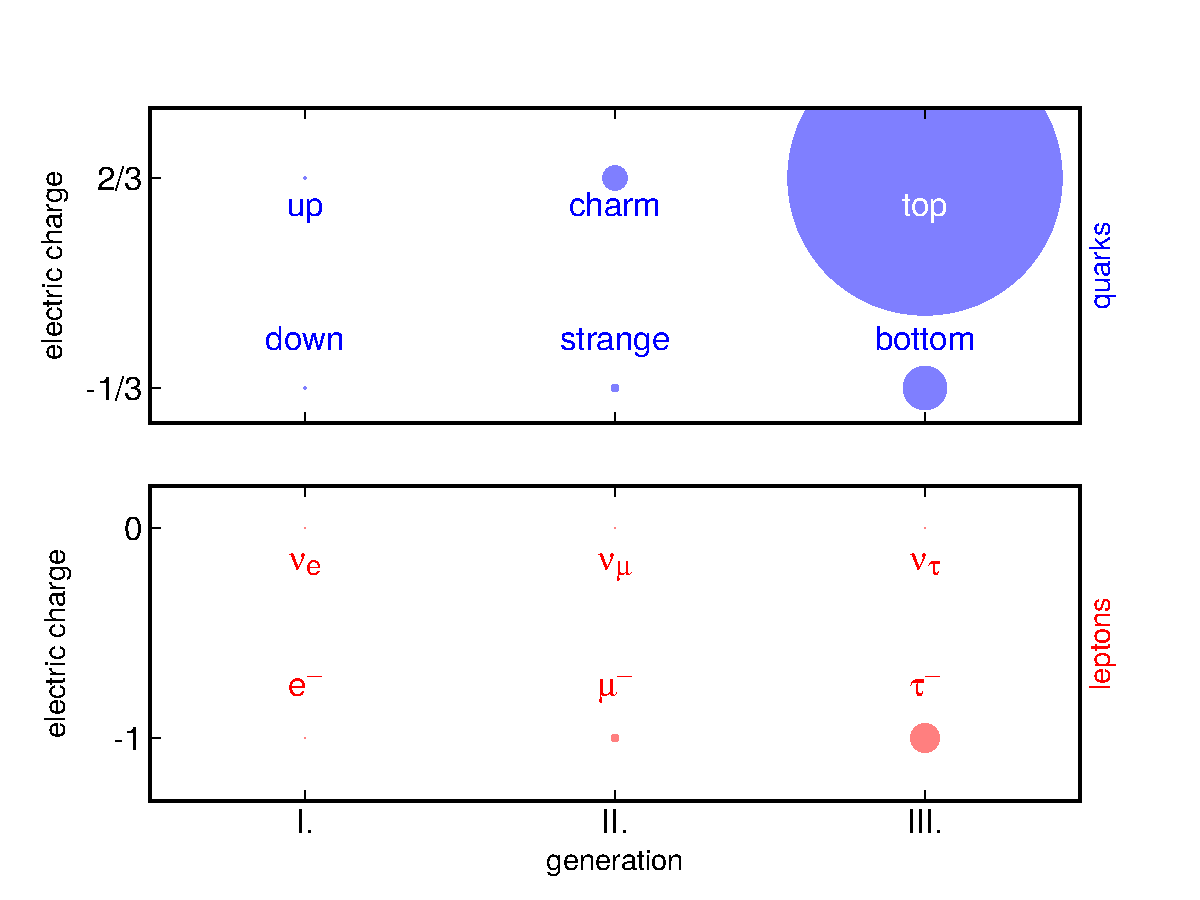
\includegraphics[width=0.95\textwidth]{figures/standardmodel/sm_fermions.pdf}
	\caption{Schematic overview of quarks and leptons, grouped by affiliation to generation and electric charge. The size of the circles is proportional to the fermion mass.}
	\label{fig:sm:fermions}
\end{figure}

There are six quark flavours, which can be grouped by their electric charge in the up-type quarks \(\Pqu_{i}\) (\(i=1, 2, 3\)) with electric charge \(\nicefrac{2}{3}\) and down-type quarks \(\Pqd_{i}\) (\(i=1, 2, 3\)) with electric charge \(\nicefrac{-1}{3}\). The up-type quarks are the up (\Pqu), charm (\Pqc), and top (\Pqt) quarks. The down-type quarks are the down (\Pqd), strange (\Pqs), and bottom (\Pqb) quarks. Quarks are the only fermions with colour charge \(q^{\alpha}, \alpha=r, g, b\), and are represented as colour charge triplets under \(\textrm{SU}(3)_{C}\)
\begin{align}
    \Pq = \begin{pmatrix} \Pq^{r} \\ \Pq^{g} \\ \Pq^{b} \end{pmatrix}.
\end{align}
The left-handed quarks carry weak isospin \(I_{3} = \pm \nicefrac{1}{2}\) and transform as doublets of up- and down-type quarks under \(\mathrm{SU}(2)_{L}\)
\begin{align}
    \begin{pmatrix} \Pqu \\ \Pqd' \end{pmatrix}_{L}, \begin{pmatrix} \Pqc \\ \Pqs' \end{pmatrix}_{L}, \begin{pmatrix} \Pqt \\ \Pqb' \end{pmatrix}_{L},
\end{align}
whereas the right-handed quarks carry weak isospin \(I_{3} = 0\) and transform as singlets
\begin{align}
\Pqu_{R}, \Pqd_{R}, \Pqc_{R}, \Pqs_{R}, \Pqt_{R}, \Pqb_{R}.
\end{align}
Here, \(\Pqd'_{i} = \Pqd', \Pqs', \Pqb'\) are the weak eigenstates, which are obtained from of the mass eigenstates \(\Pqd_{i} = \Pqd, \Pqs, \Pqb\) by a rotation \(\Pqd'_{i} = \sum_{j} V_{ij} d_{j}\) with the Cabibbo-Kobayashi-Maskawa mixing matrix~\cite{Cabibbo1963,Kobayashi1973,Tanabashi2018}
\begin{align}
\begin{split}
    V &= \begin{pmatrix} %
    	\Vud & \Vus & \Vub \\%
    	\Vcd & \Vcs & \Vcb \\%
    	\Vtd & \Vts & \Vtb%
    \end{pmatrix} \\
       &=  %
    \begin{pmatrix}%
    	\num{0.97417} \pm \num{0.00021} & \num{0.2248} \pm \num{0.0006} & \num{0.000409} \pm \num{0.000039} \\%
    	\num{0.220} \pm\num{0.005} & \num{0.995} \pm \num{0.016} & \num{0.00405} \pm \num{0.0015} \\%
    	\num{0.0082} \pm \num{0.0006} & \num{0.04} \pm \num{0.0027} & \num{1.0009} \pm \num{0.031}%
    \end{pmatrix}.
\end{split}
\end{align}
Quarks participate in strong, electromagnetic, and weak interactions.

There are six lepton flavours, which also can be grouped by their electric charge in the charged leptons and neutral leptons. The charged leptons are the electron (\Pem), the muon (\Pgmm), and the tau lepton (\Pgtm). They carry the electromagnetic charge \(q_{\Plpm_{i}} = - 1\). The neutral leptons are the associated neutrinos \Pgne, \Pgngm, \Pgngt.
The left-handed leptons carry weak isospin \(I_{3} = \pm \nicefrac{1}{2}\) and transform as doublets under \(\mathrm{SU}(2)_{L}\)
\begin{align}
\begin{pmatrix} \Pgne \\ \Pem \end{pmatrix}_{L}, \begin{pmatrix} \Pgngm \\ \Pgmm \end{pmatrix}_{L}, \begin{pmatrix} \Pgngt \\ \Pgtm \end{pmatrix}_{L},
\end{align}
whereas the charged right-handed leptons carry weak isospin \(I_{3} = 0\) and transform as singlets
\begin{align}
\Pem_{R}, \Pgmm_{R}, \Pgtm_{R}.
\end{align}
To date, neither right-handed neutrinos nor left-handed anti-neutrinos have been observed. The charged leptons participate in electromagnetic and weak interactions, while the neutrinos only participate in weak interactions.


\section{The Standard Model in the Lagrangian formalism}
\label{sec:sm:lagrangian}
The SM is elegantly and concisely formulated in the Lagrangian formalism of quantum field theory. The particles are described by quantum fields, which are operators on the Hilbert space of particle states. The fermions are described by spin-\(\nicefrac{1}{2}\) spinor fields \(\psi(x)\). The gauge bosons are described by spin-1 vector fields \(A_{\mu}\). The Higgs boson, the only spin-\(0\) particle in the SM, is described by a scalar field \(\phi(x)\).

Remarkably, all dynamics of elementary particles are determined by the action
\begin{align}
    S[\varphi] = \int \dd{x} \mathcal{L}\left(\varphi(x), \partial_{\mu}\varphi(x)\right),
\end{align}
where \(\varphi\) is a generic field variable and \(\mathcal{L}\left(\varphi(x)\right)\) is the Lorentz-invariant Lagrangian (density). The equations of motions for elementary particles are obtained by the means of Hamilton's principle
\begin{align}
    \delta S = S[\varphi + \delta \varphi] - S[\varphi] = 0.
\end{align}

The Lagrangian of the SM consists of the four parts\footnote{In principle, \(\mathcal{L}\), could be extended by a term associated with the strong interaction, violating charge and parity (CP) symmetry. As there is no evidence for CP violation in strong interactions, this term is neglected. Also, additional gauge-fixing terms, e.g. \(\delta \mathcal{L} = - (\partial_{\mu} A^{\mu})^2 / 2 \zeta\) with the parameter \(\zeta\) for a gauge field \(A_{\mu}\), are neglected in the following discussion.}
\begin{align}
    \mathcal{L} = \mathcal{L}_{\text{Gauge}} + \mathcal{L}_{\text{Fermion}} + \mathcal{L}_{\text{Higgs}} + \mathcal{L}_{\text{Yukawa}},
\end{align}
which are described in the following paragraphs.

\subsection{Gauge boson kinetic term}
\label{sec:sm:lagrangian:boson}
The gauge-invariant gauge boson kinetic term
\begin{align}
    \mathcal{L}_{\text{Gauge}} = - \frac{1}{4} G_{\mu\nu}^{a} G^{\mu\nu}_{a} - \frac{1}{4} W^{i}_{\mu\nu} W_{i}^{\mu\nu} - \frac{1}{4} B_{\mu\nu} B^{\mu\nu}
\end{align}
is required to promote the gauge bosons, which emerge from the gauge principle, to dynamical fields. It consists of the field strength tensors of the strong interaction
\begin{align}
    G_{\mu\nu}^{a} = \partial_{\mu} G_{\nu}^{a} - \partial_{\nu}G_{\mu}^{a} - g_s f_{abc} G_{\mu}^{b} G_{\nu}^{c},
\end{align}
where \(f_{abc}\) denotes the structure constants of the \(\textrm{SU}(3)_{C}\) group, and the field strength tensors for the electroweak gauge bosons
\begin{align}
    W^{i}_{\mu\nu} &= \partial_{\mu} W_{\nu}^{i} - \partial_{\nu} W_{\mu}^{i} + g W_{\mu}^a,
\end{align}
where the totally antisymmetric tensor \(\varepsilon_{ijk}\) denotes the structure constants of the \(\textrm{SU}(2)_{L}\) group. The terms associated with the structure constants are responsible for the non-trivial gauge transformations and introduce the three- and four-point direct interactions among the weak gauge bosons and among the gluons. No explicit mass terms are present in \(\mathcal{L}_{\text{Gauge}}\), as their presence would violate gauge invariance. They are introduced via electroweak spontaneous symmetry breaking.

\subsection{Fermion kinetic and interaction term}
\label{sec:sm:lagrangian:fermion}
The fermion kinetic term introducing interactions with the gauge bosons
\begin{align}
    \mathcal{L}_{\text{Fermion}} = \sum_{j} \overline{\psi}_{L}^{j} i \gamma^{\mu} D_{\mu}^{L} \psi_{L}^{j} + \sum_{j, \sigma} \overline{\psi}_{R\sigma}^{j} i \gamma^{\mu} D^{R}_{\mu} \psi^{j}_{R\sigma}
\end{align}
describes the left-handed fermion fields \(\psi_{L}^{j, T} = (\psi_{L+}^{j} \psi_{L-}^{j})\) and the right-handed fermion fields \(\psi_{R}^{j\sigma}\). They carry the generation index \(j\) and the component index \(\sigma=\pm\), which denotes up-type fermions (\(+\)) and down-type fermions (\(-\)). Their interactions with the gauge bosons via the minimal substitution rule is introduced by the covariant derivative
\begin{align}
    D^{L, R}_{\mu} = \partial_{\mu}  - i g_{s} T_{a} G^{a}_{\mu} - i g I^{L,R}_{j} W^{j}_{\mu} + i g' \frac{Y}{2} B_{\mu}.
\end{align}
\(T_{a}\), \(I^{L}_{a}\), and \(\frac{Y}{2}\) are the generators of the groups \(\textrm{SU}(3)_{C}\), \(\textrm{SU}(2)_{L}\), and \(\textrm{U}(1)_{Y}\), respectively. They are defined by \([T_{a}, T_{b}] = i f_{abc} T_{c}\) and \([I^{L}_{a}, I^{L}_{b}] = i \varepsilon_{abc} I^{L}_{c}\). In the triplet representation, \(T_{a} = \frac{1}{2} \lambda_{a}\) can be written with the Gell-Mann matrices \(\lambda_{a}, a=1, \dots, 8\). Similarly, \(I_{j}^{L} = \frac{1}{2} \sigma_{j}\) can be written in the doublet representation with the Pauli matrices \(\sigma_{j}, j=1,2,3\). For the sake of consistent notation, the associated term for right-handed particles is \(I_{j}^{R} = 0\).
No mass terms for Fermions are included in \(\mathcal{L}_{\text{Fermion}}\), as they would mix left- and right-handed fields and would explicitly break gauge invariance. The fermion mass terms are introduced via gauge-invariant Yukawa interactions between the fermions and the Higgs field.

\subsection{The Higgs mechanism in the Standard Model}
\label{sec:sm:lagrangian:higgs}
The Higgs field term
\begin{align}
    \mathcal{L}_{\textrm{Higgs}} = (D_{\mu} \phi)^{\dag} (D^{\mu} \phi) - V(\phi)
\end{align}
introduces a complex scalar Higgs doublet \(\Pphi = \begin{pmatrix} \Pphi^{+} \\ \Pphi^{0} \end{pmatrix}\) with hypercharge \(Y=1\) and the covariant derivative
\begin{align}
    D_{\mu} = \partial_{\mu} + i g \frac{1}{2} \sigma_{j} W_{\mu}^{j} + i g' \frac{Y}{2} B_{\mu}.
\end{align}
The Higgs potential
\begin{align}
    V(\Pphi) = \mu^2 \Pphi^{\dag} \Pphi + \frac{\lambda}{4} (\Pphi^{\dag} \Pphi)^2.
\end{align}
has two free parameters \(\mu^2\) and \(\lambda > 0\). For \(\mu^2 > 0\), \(\mathcal{L}_{\textrm{Higgs}}\) describes a scalar field with mass \(\mu\) which can self-interact via a four-point interaction vertex with coupling \(\lambda\) and whose ground state corresponds to \(\phi = 0\). More interesting is the case \(\mu^2 < 0\), which is shown in \Cref{fig:sm:higgs-potential} for a specific choice of these parameters, as it allows introducing mass terms for the gauge bosons via spontaneous symmetry breaking while respecting the \(\text{SU}(2)_{L} \times \textrm{U}(1)_{Y}\) gauge-invariance.
\begin{figure}[htbp]
    \centering
    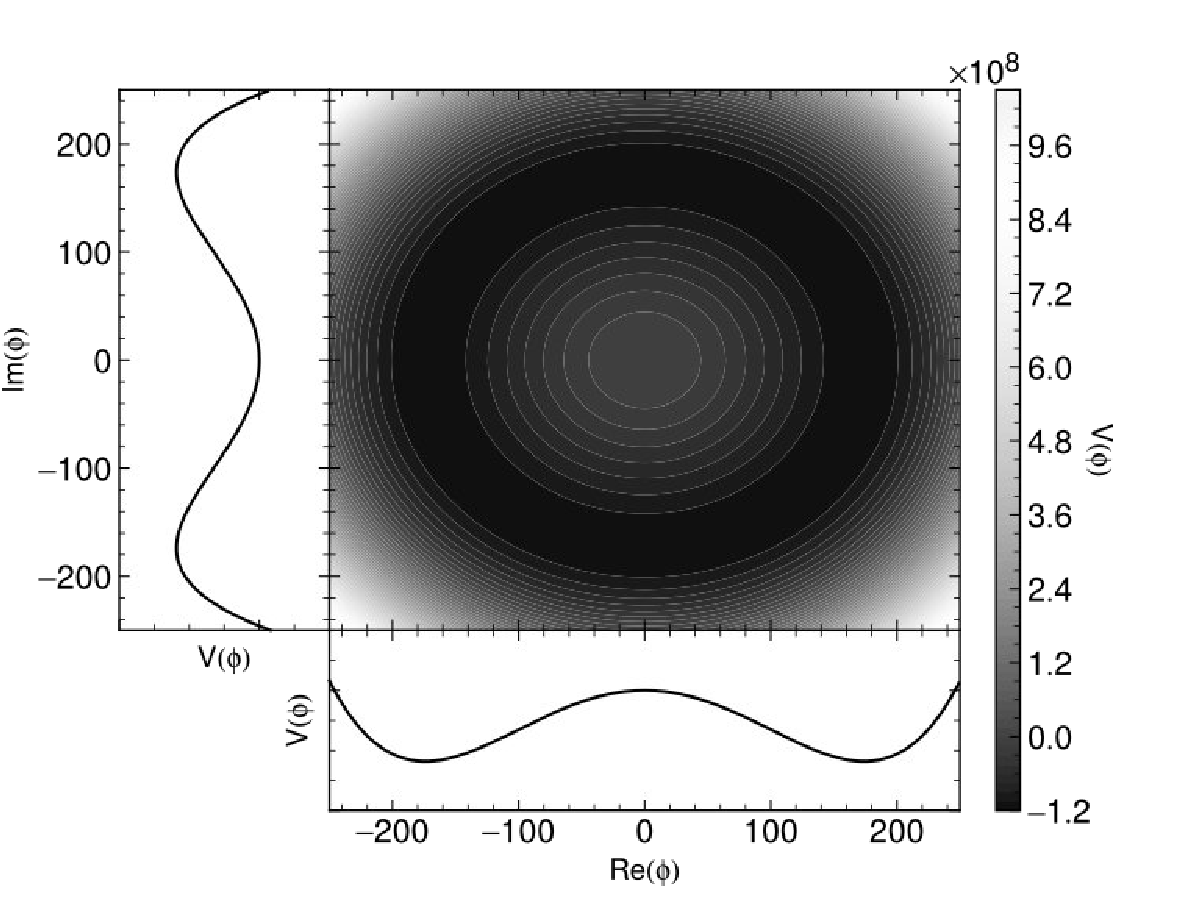
\includegraphics[width=0.95\textwidth]{figures/standardmodel/sm_higgs_sw.pdf}
    \caption{The Higgs potential \(V(\phi)\) with parameters \(\mu^2 = -(\SI{125}{\giga\electronvolt})^2 / 2\) and \(\lambda = 0.13\) is shown in dependency of the real and imaginary part of \(\phi\). For this choice of parameters \(\mu^2 < 0\) and \(\lambda > 0\) the potential assumes its minimum at the circle with radius \(v / \sqrt{2} = \SI{246}{\giga\electronvolt} / \sqrt{2}\), which is defined by the vacuum expectation value \(v\).}
    \label{fig:sm:higgs-potential}
\end{figure}
The potential \(V(\phi)\) is minimised by all field configurations on the circle in the \(\text{Re}(\phi)\)-\(\text{Im}(\phi)\)-plane defined by \(\abs{\phi}^2 = 2 \mu^2 / \lambda\).
Choosing the specific real and electrically neutral ground state configuration
\begin{align}
    \phi_0 = \expval{\phi}{0} = \frac{1}{\sqrt{2}} \begin{pmatrix} 0 \\ v \end{pmatrix},
\end{align} spontaneously breaks the \(\textrm{SU}(2)_{L} \times \textrm{U}(1)_{Y}\) symmetry of the Lagrangian. Here, \(v = 2 \mu / \sqrt{\lambda}\) denotes the vacuum expectation value.
Although the specific choice of the ground state breaks the symmetry, the Lagrangian and the physical system are still invariant under symmetry operations%
    \footnote{This statement can be illustrated by considering a scalar field \(\phi\) and a potential \(V = V(\abs{\phi})\). The potential possesses a \(\textrm{U}(1)\) symmetry and the associated Lagrangian density \(\mathcal{L} = \abs{\partial_{\mu} \phi}^2 - V(\abs{\phi})\) is symmetric under transformations \(\phi \mapsto \phi' = e^{i \alpha} \phi\). If the minimum \(\phi_{0} = v\) of the potential \(V\) does not occur at \(v=0\), the symmetry of the ground state is broken \(\phi_{0}' = e^{i \alpha} v \neq \phi_{0}\).}.

The \(U(1)_{Q}\) symmetry of the vacuum, corresponding to the conservation of electric charge, remains unbroken, as the operator associated with electric charge \(Q = I_3 + \frac{Y}{2}\) leaves the ground state invariant.

Perturbative calculations should involve expansions around the ground state. The Higgs doublet can be expanded around the ground state \(\phi_{0}\) in the real field \(h(x)\) and the three real fields \(\theta^{i}(x)\)
\begin{align}
\phi(x) = \frac{1}{\sqrt{2}} \begin{pmatrix} 0 \\ v + h(x) \end{pmatrix} e^{i I^{L}_{j} \theta^{j}(x)}.
\end{align}
In the unitary gauge, \(\theta^{j}(x) = 0\), the massless Goldstone modes \(\theta^{j}(x)\) are absorbed by the weak gauge bosons, giving them a longitudinal polarisation. The Higgs field term after spontaneous symmetry breaking now reads
\begin{align}
\begin{split}
    \mathcal{L}_{\textrm{Higgs}} = & \frac{1}{2} \partial^{\mu} h \partial_{\mu} h - \mu^2 h^2 \\
    & +  \frac{g^2}{8} v^2 \left(W_{\mu}^{+} W^{\mu +} + W_{\mu}^{-} W^{\mu -} \right) + \frac{g^2}{4 \cos^2 \theta_{W}} v^2 Z_{\mu}Z^{\mu} \\
    & + (2vh + h^2) \left(\frac{g^2}{4} W_{\mu}^{+} W^{\mu -} + \frac{g^2}{8 \cos^2 \theta_{W}} Z_{\mu}Z^{\mu}\right) \\
    & + \lambda v h^3 + \frac{\lambda}{4} h^4.
\end{split}
\label{eq:sm:lagrangian:higgs:broken}
\end{align}
It explicitly describes (with the number corresponding to the line in \Cref{eq:sm:lagrangian:higgs:broken})
\begin{enumerate}
    \item the massive real scalar Higgs boson with explicit kinetic and mass term,
    \item the mass terms \(m_{\PWpm} = g^2 v^2 / 4\) and \(m_{\PZ} = g^2 / 8 \cos^2 \theta_{W}\) for the massive weak vector gauge bosons \PWpm and \PZ, respectively,
    \item interactions between the Higgs boson and the weak vector gauge bosons, and
    \item triple and quartic couplings of the Higgs boson.
\end{enumerate}

After electroweak symmetry breaking the associated four gauge fields are
\begin{align}
    W^{\pm}_{\mu} &= \frac{1}{\sqrt{2}} \left(W^{1}_{\mu} \pm W^{2}_{\mu} \right), \\
    Z_{\mu} &= W_{\mu} \cos \theta_{W} - B_{\mu} \sin \theta_{W} \\
    A_{\mu} &= B_{\mu} \cos \theta_{W} + W_{\mu}^{3} \sin \theta_{W}
\end{align}
where \(Z_{\mu}\) and \(W^{\pm}_{\mu}\) are the neutral and charged massive gauge bosons mediating the weak interaction. \(A_{\mu}\) is the photon mediating the electromagnetic interaction. The Weinberg angle \(\theta_{W}\) is defined by the couplings \(g\) and \(g'\) of \(\mathrm{SU}(2)_{L} \times \mathrm{U}(1)_{Y}\)
\begin{align}
    \sin \theta_{W}  = \frac{g'}{\sqrt{g^2 + g'^2}} \quad \cos \theta_{W} = \frac{g}{\sqrt{g^2 + g'^2}}.
\end{align}
The electric charge is related to the couplings \(g\) and \(g'\) and to the Weinberg mixing angle by
\begin{align}
    e = g \sin \theta_{W} = g' \cos \theta_{W}.
\end{align}
The electromagnetic coupling constant is customarily expressed by the fine structure constant \(\alpha_{\text{EM}} = e^2 / 4 \pi\).

\subsection{Yukawa interactions between fermions and the Higgs field}
\label{sec:sm:lagrangian:yukawa}
The Yukawa term in unitary gauge (neglecting flavour mixing in the quark sector)
\begin{align}
    \mathcal{L}_{\text{Yukawa}} = - \sum_{f} m_{f} \overline{\psi}_{f} \psi_{f} - \sum_{f} \frac{m_{f}}{v} \overline{\psi}_{f} \psi_{f} h
\end{align}
contains the mass terms \(m_{f} = y_{f} v / \sqrt{2}\), which relate the individual Yukawa coupling constants \(y_{f}\) to the mass of the charged fermions \(f = \Pqu, \Pqd, \dots, \Pgt\). The interactions between the massive fermions and the Higgs boson occur with coupling constants proportional to the fermion masses.

\section{Phenomenology of the Standard Model}
\label{sec:sm:phenomenology}
The non-Abelian structure of the \(\mathrm{SU}(3)_{C}\) and \(\mathrm{SU}(2)_{L}\) symmetry groups results in distinctive properties of strong and weak interactions. The non-trivial transformations of the strong and weak gauge bosons under their respective symmetry groups allow them to interact directly in three- or four-point interactions.

In particular, the direct coupling of gluons has dramatic implications for the strong interaction, which become apparent in considering the effects of charge screening. As an example, consider an electric probe charge near a charged source. The coupling constant of the electromagnetic interaction increases at small distances to a charged source due to the screening of \HepProcess{\Pep\Pem} pairs of the vacuum. This behaviour is known as ``running coupling''. The coupling constant of the strong interaction shows precisely the opposite behaviour, as the vacuum is not only a polarisable medium due to \HepProcess{\Pq\Paq} pairs but also due to gluon pairs. The gluons spread out the effective colour charge of the quark and counteract the effect from quark pairs. The resulting behaviour of quarks interacting at small length scale (high energy) as nearly free particles is known as \emph{asymptotic freedom} and is essential for turning quantum chromodynamics into a quantitative calculational scheme predicting the interactions at particle colliders.

The second defining feature of the strong interaction is the \emph{colour confinement hypothesis}, stating that only colour-singlet states are observed. As a consequence, no free quarks have been observed to date but only bound states of two or more quarks. These bound states are collectively called \emph{hadrons}, with the \emph{baryons} states \(B\) and the \emph{mesons} states \(M\), which are defined by
\begin{align}
    B &= \frac{1}{\sqrt{6}} \varepsilon^{\alpha \beta \gamma} \ket{q_{\alpha} q_{\beta} q_{\gamma}} \\
    M &= \frac{1}{\sqrt{3}} \delta^{\alpha \beta} \ket{q_{\alpha} \overline{q}_{\beta}}.
\end{align}
Recently, exotics bound states of four~\cite{Aaij2017,Aaij2020} or five quarks~\cite{Aaij2015} have been observed, which are in agreement with the colour confinement hypothesis.
Another consequence of the confinement hypothesis, which strikingly manifests in high-energy hadron collision events, is the formation of jets~\cite{Sterman1977}. Jets are collimated sprays of particles emerging from coloured states in a similar manner as a decelerating electric charge emits photons via Bremsstrahlung. When a quark anti-quark pair is separated, their colour interaction increases due to the ``running coupling'' and squeezes the colour field lines into tube-like regions until the increasing potential energy suffices for the creation of another quark anti-quark pair. The repeated formation of clusters of quarks and gluons forming hadrons is called \emph{hadronisation}.


The free parameters SM are empirically determined with great precision. The discovery of the Higgs boson in 2012~\cite{HIGG-2012-27,CMS-HIG-12-028} concluded the experimental inventory of all SM particles and corroborated the local gauge theory with spontaneous symmetry breaking as the empirically adequate description of fundamental interactions.

% A particular choice of a set of free parameters, which are (in principle) directly accessible by experiment is reported in \Cref{tab:sm:parameters}~\cite{Tanabashi2018}.
% \begin{table}[htb]
% \caption{Empirically determined free parameters of the SM}
% \label{tab:sm:parameters}
% \centering
% \begin{tabular}{l r}
% \toprule
% parameter &  value \\
% \midrule
% fine-structure constant \(\alpha_{\text{EM}}\) & \num{0.0072973525693}\\
% Weinberg mixing angle \(\theta_{W}\) & \num{0.23122}\\
% coupling constant of strong interaction \(\alpha_{s}\) & \num{0.1182}\\
% Higgs potential vacuum expectation value \(v\) & \SI{246}{\giga\electronvolt}\\
% Higgs boson mass & \SI{125}{\giga\electronvolt}\\
% up quark mass \(m_{\Pqu}\) & \SI{2.2}{\mega\electronvolt} \\
% down quark mass \(m_{\Pqd}\) & \SI{4.7}{\mega\electronvolt} \\
% strange quark mass \(m_{\Pqs}\) & \SI{96}{\mega\electronvolt}\\
% charm quark mass \(m_{\Pqc}\) & \SI{1.27}{\giga\electronvolt}\\
% bottom quark mass \(m_{\Pqb}\) & \SI{4.18}{\giga\electronvolt}\\
% top quark mass \(m_{\Pqt}\) & \SI{173.21}{\giga\electronvolt}\\
% electron mass \(m_{\Pem}\) & \SI{0.51}{\mega\electronvolt}\\
% muon mass \(m_{\Pgmm}\) & \SI{105.66}{\mega\electronvolt}\\
% tau lepton mass \(m_{\Pgtm}\) & \SI{1.776}{\giga\electronvolt}\\
% CKM matrix mixing angle \(\theta_1\) & (not discussed) \\
% CKM matrix mixing angle \(\theta_1\) & (not discussed) \\
% CKM matrix mixing angle \(\theta_1\) & (not discussed) \\
% CKM matrix CP-violating phase \(\delta_{13}\) & (not discussed)\\
% possible CP-violating strong-interaction parameter & (not discussed)\\
% \bottomrule
% \end{tabular}
% \end{table}
% Once the free parameters are know, the predictions of the SM can be tested with great precision.

The impressive success of the SM in accurately describing the observations across 15 orders of magnitude is demonstrated in cross-section measurements of SM processes by the ATLAS experiment at the Large Hadron Collider, which is shown in \Cref{fig:sm:atlas-measurement}.

\begin{figure}[htbp]
    \centering
    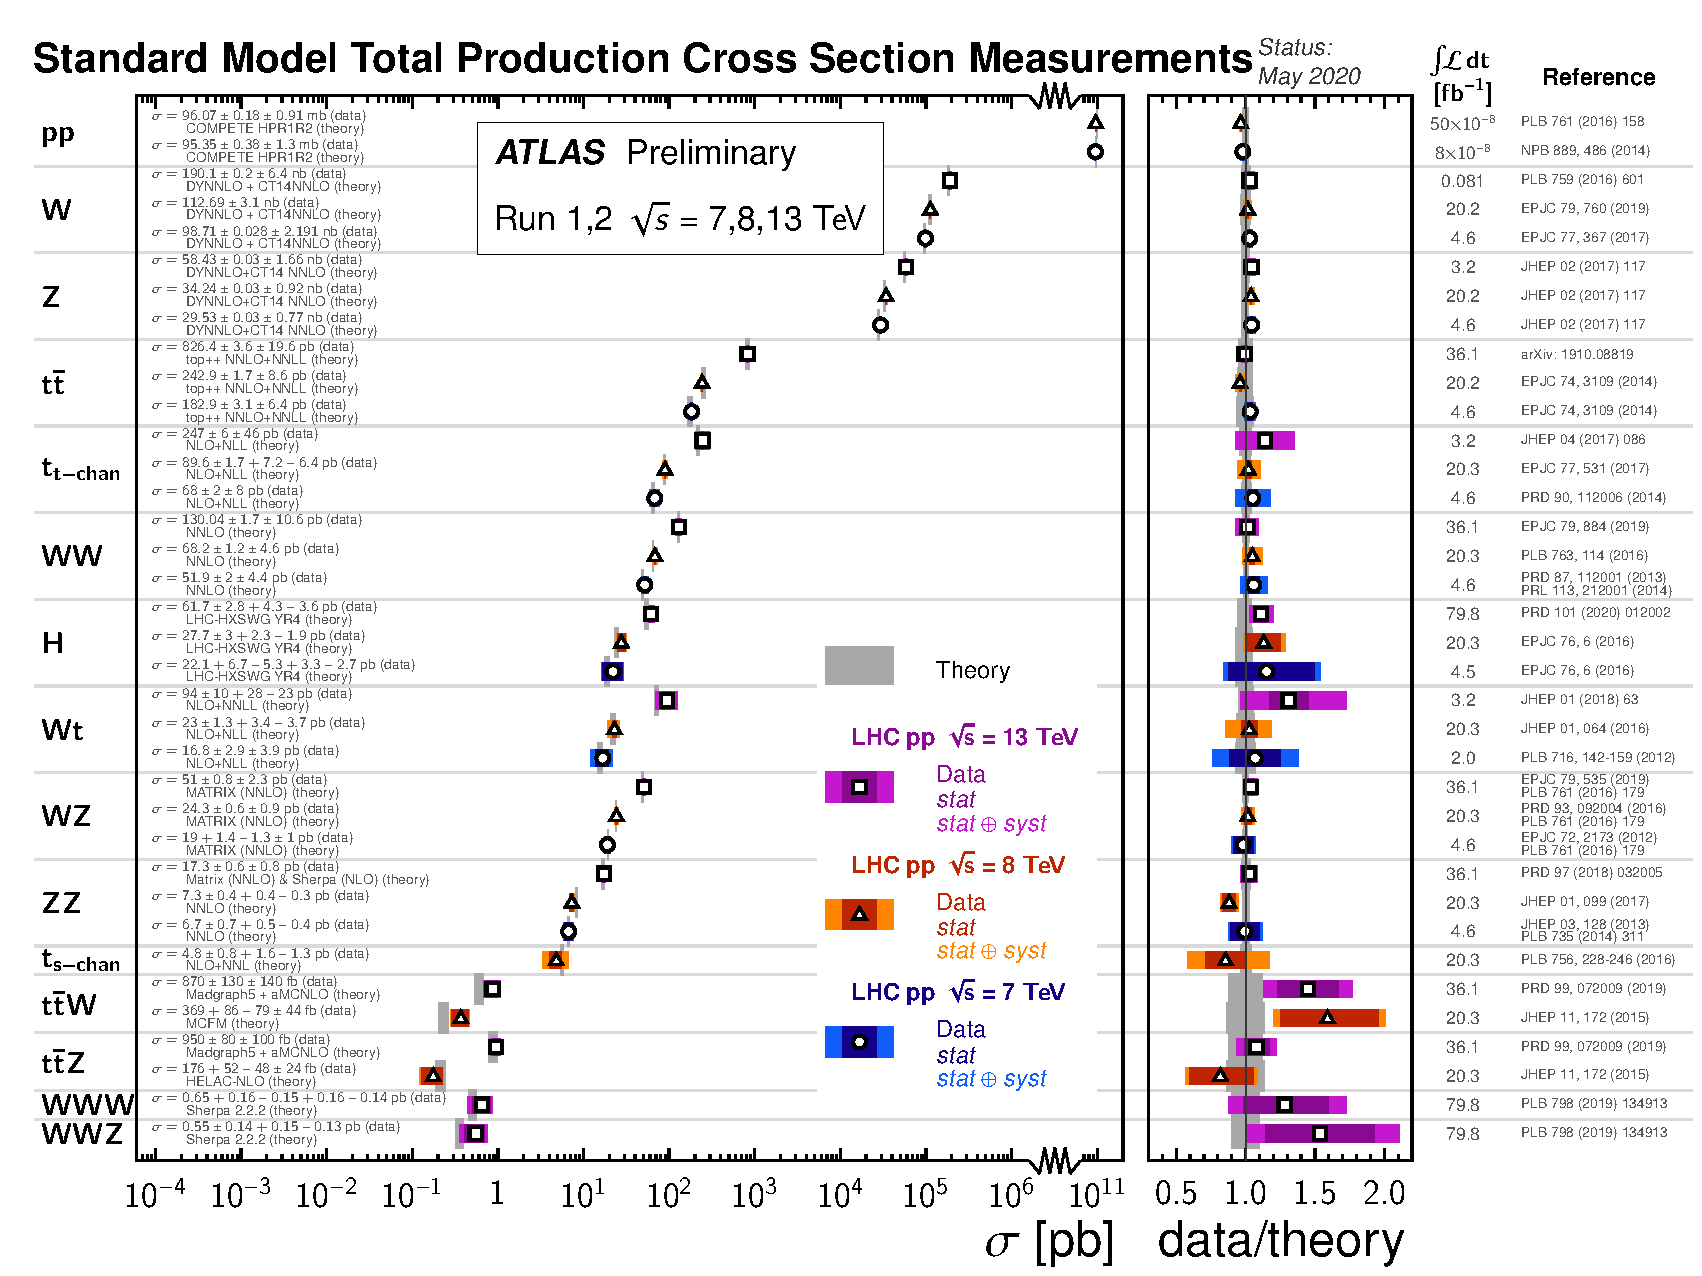
\includegraphics[width=1.05\textwidth]{figures/standardmodel/sm_processes_atlas_fig_02.pdf}
    \caption{Summary of several Standard Model total production cross-section measurements, corrected for branching fractions, compared to the corresponding theoretical expectations and ratio with respect to best theory prediction. Figure reproduced from Ref.~\cite{ATL-PHYS-PUB-2020-010}.}
    \label{fig:sm:atlas-measurement}
\end{figure}

\section{Limitations of the Standard Model}
\label{sec:sm:limitations}
Despite the SM's success in providing the most complete and solid theoretical framework to date, several observed phenomena cannot be explained by the SM. They suggest the existence of a more fundamental theory, of which the SM is the low-energy limit. This section presents a non-exhaustive account of both fundamental and aesthetic shortcomings of the SM and open questions in fundamental physics.
\begin{itemize}
    \item The SM only describes three out of the four known fundamental interactions. Gravity is most successfully described by Einstein's theory of General Relativity, which is mathematically incompatible with the formulation of the SM as a renormalisable quantum field theory~\cite{DeWitt1967,DeWitt1967-2,DeWitt1967-3,Feynman2018}. At present, this is merely a theoretical problem, as current experiments are either sensitive to quantum effects, where the minuteness of particle masses justifies neglecting gravity, or to the gravitational pull of extended objects, which do not show quantum behaviour. Eventually, a complete and consistent quantum theory of gravity is required for a truly fundamental description of Nature.
    \item In its original formulation, the SM does not account for neutrino masses. The experimental observation of neutrino flavour oscillations indicates that neutrinos have non-vanishing mass~\cite{GonzalezGarcia2008}. The mixing of the neutrino-mass eigenstates to give the weak neutrino eigenstates is described --- similarly to the CKM matrix --- by the Pontecorvo–Maki–Nakagawa–Sakata matrix~\cite{Pontecorvo1967,Maki1962}. The direct measurement of the neutrino masses and the determination of the neutrino mass hierarchy is a current object of research~\cite{Aker2020}.
    \item The vast prevalence of matter over antimatter in the universe is puzzling, as it is natural to assume that in the early universe both matter and antimatter were created in equilibrium. The violation of CP symmetry could explain the matter-antimatter asymmetry~\cite{Sakharov1991}. However, the CP violation in the SM, appearing as a complex phase in the quark mixing matrix of the weak interaction, is by far not sufficient to explain the observed asymmetry.
    \item The energy scale of electroweak symmetry breaking is \(\mathcal{O}(\SI{100}{\giga\electronvolt})\). If the SM were the fundamental theory of Nature, it would be expected to describe phenomena up to the Planck scale, defined by \(m_{\text{Planck}} = 1 / \sqrt{8 \pi G} = \mathcal{O}(\SI{e18}{\giga\electronvolt})\), where \(G\) denotes Newton's constant. The scalar Higgs boson mass receives quadratically divergent radiative loop corrections \(\Delta m_{h}\) from all particles interacting with the Higgs field. Including these corrections, the square of the Higgs boson mass is
    \begin{align}
        m_{h}^{2} = (m_{h}^{\text{bare}})^2 + \Delta m_{h}^2 = (m_{h}^{\text{bare}})^2 + \text{const.} \times \Lambda^2,
    \end{align}
    where \(\Lambda\) is the fundamental scale parameter of the theory.
    Given the measured Higgs boson mass  \(m_{h} = \SI{125}{\giga\electronvolt}\), the theory requires a precise fine-tuning of \(m_{h}^{\text{bare}}\) over more than \(10^{36}\) orders of magnitude, which is not considered to be aesthetic~\cite{Murayama2000}.
    \item Astrophysical observations strongly indicate that the baryonic matter described by the SM is insufficient to account for phenomena on scales ranging from galactic rotation curves to cosmology. An additional matter component, the so-called dark matter is required to describe the observed phenomena accurately. \Cref{sec:dm} provides a detailed discussion of the research programme defined by dark matter.
\end{itemize}

% \chapter{Dark matter}
\label{sec:dm}

\cleanchapterquote{We live on a placid island of ignorance in the midst of black seas of infinity, and it was not meant that we should voyage far.}{Howard Phillips Lovecraft}{The Call of Cthulhu, in Weird Tales Volume XI Number 2. Indianapolis: Popular Fiction Publishing Co., 1928}


\section{Introduction}
\label{sec:dm:intro}
Astrophysics and cosmological observations supply compelling evidence that the particle content of the SM can only account for a small fraction of the matter-energy-density of the universe. Several extensions of the SM suggest the existence of invisible particles, which can account for the missing component as \emph{dark matter}. General relativity, the currently established theory of gravity, is only able to describe and explain the observed phenomena if there is dark matter in the universe. Although it has been almost a hundred years after dark matter's initial discovery, its particle nature remains an open question.

The term dark matter denotes a non-luminous and non-absorbing matter component. It was first coined in the year 1922 by the Dutch astronomer Jacobus Kapteyn in a study estimating the density of matter near the Sun~\cite{Kapteyn1922}.
The earliest, perhaps even the most convincing evidence for the existence of dark matter came from the observation that astrophysical objects move faster than one would expect if they were subject only to the gravitational interaction of visible objects. These observations disagree with the predictions of the well-established theories of gravitation.

However, the falsification of a theory by empirical tests is necessarily ambiguous, as every interpretation depends on further assumptions~\cite{Duhem1954}. For instance, the observed anomalies could also be explained by the presence of additional, yet undiscovered gravitational potentials. Then, do such anomalies falsify the theory of gravitation or do they point towards unseen --- in other words ``dark'' --- celestial objects?

Two historical examples show how observations which seemingly refute the established theories advance scientific understanding~\cite{Bertone2005}. Both examples consider observed anomalies in the motion of the planets in the Solar System.
\begin{enumerate}
    \item In the case of the anomalous motion of Uranus, the French mathematician Urbain Le Verrier chose not to abandon Newtonian gravity. Instead, he confronted the troublesome orbit by conjecturing another planet --- Neptune. Its discovery would add another planet to the inventory of our Solar System and corroborate Newtonian gravity. Indeed, the German astronomer Johann Gottfried Galle discovered the planet Neptune in 1846 within the same evening that Le Verrier's letter reached him and proved his predictions to be true~\cite{Galle1846,Leverrier1910}.
    \item In a similar manner, Le Verrier tried to address the anomalies in the motion of Mercury, which were observed the first time in 1859, by postulating the existence of the hypothetical planet Vulcan. Conversely, this ``dark planet'' was never discovered. Consequentially, the research programme defined by Newtonian gravity had to be abandoned. The advent of Einsteinian gravity solved the problem by accurately predicting the anomalous perihelion shift of Mercury without the need for postulating new objects~\cite{Clemence1947}.
\end{enumerate}

The verdict on whether dark matter defines a progressive research programme~\cite{Lakatos1976} or whether it will be eventually abandoned in favour of a new theory of gravitation is ultimately decided by experimental searches for dark matter. To date, it remains an open problem in fundamental physics.


\section{Cosmology in a nutshell}
\label{sec:dm:cosmology}
The present knowledge about composition, evolution and structure of the universe is described by the \(\Lambda\)-CDM model. The model is based on the presence of a non-vanishing cosmological constant \(\Lambda\) and cold dark matter, which shows a small velocity dispersion in contrast to warm or hot dark matter. The dark matter paradigm is at the heart of the currently established cosmological model, which describes the evolution of the universe from an initial, highly compressed state to its present state.
According to the \(\Lambda\)-CDM model, the ordinary baryonic matter, building blocks to humankind and its terrestrial environment, only constitutes roughly \SI{5}{\percent} of the universe's matter-energy content. Another \SI{25}{\percent} is comprised of dark matter. The remaining \SI{70}{\percent} is referred to as dark energy.
The model is able to give an account of the thermal history of the universe and explains the universe's observed properties. It correctly predicts the observed relic abundances of light elements and provides an interpretation of the cosmic microwave background radiation in terms of fundamental cosmological parameters. Simulations based on the \(\Lambda\)-CDM model can reproduce the observed large scale structure of the universe.

The \(\Lambda\)-CDM model is based on three fundamental building blocks:
\begin{enumerate}
    \item Einstein's field equations of General relativity
        \begin{align}
            R_{\mu \nu} - \frac{1}{2} R g_{\mu \nu} + \Lambda g_{\mu \nu} = \frac{T_{\mu \nu}}{M_{\text{Pl}}^2},
        \end{align}
        \begin{itemize}
            \item where \(R_{\mu \nu} = R^{\alpha}_{\mu \alpha \nu}\) is the Ricci tensor, the only independent trace of the curvature tensor \(R^{\alpha}_{\mu \beta \nu}\),
            \item \(R = R_{\mu}^{\mu}\) is the Ricci scalar,
            \item \(\Lambda\) is the so-called cosmological constant, a measure for the accelerated expansion of the universe due to the vacuum energy,
            \item \(M_{\text{Pl}} = 1 / \sqrt{8 \pi G}\) is the reduced Planck mass defined by Newton's constant \(G\), and
            \item \(T_{\mu \nu}\) is the energy-momentum tensor.
        \end{itemize}
    \item the Friedmann-Lemaître-Robertson-Walker (FLRW) metric defined by the line element
        \begin{align}
            \dd{s}^2 = \dd{t}^2 - a(t)^2 \left(\frac{\dd{r}^2}{1 - \kappa r^2} + r^2 \dd{\theta}^2 + r^2 \sin{(\theta)}^2 \dd{\phi}^2\right),
        \end{align}
        \begin{itemize}
            \item where \(a(t)\) is the spatial scale factor describing the relative expansion of the universe
            \item \(\kappa\) is the curvature parameter describing the spatial curvature of the universe. \(\kappa\) can take values of \num{0}, \num{+1}, and \num{-1}, corresponding to a flat, a closed, or an open universe, respectively.
        \end{itemize}
    \item the equation of state relating pressure \(p_{j}\) and energy density \(\rho_{j}\) of a species \(j\)
        \begin{align}
            p_{j}(t) = w_{j} \rho_{j},
        \end{align}
        where \(w_{j}\) is a dimensionless constant, which is
        \begin{align}
            w_{j} = \begin{cases}
                0 & \text{for non-relativistic matter} \\
                \nicefrac{1}{3} & \text{for relativistic radiation} \\
                -1 & \text{for vacuum energy}.
                \end{cases}
        \end{align}
\end{enumerate}

These building blocks themselves can be derived from fairly general principles, which are based on empirical observations. Einstein's field equations can be derived from almost first principles, assuming invariance under general coordinate transformations and equivalence to Newton's law in the limit of weak gravitational fields.
The FLRW metric is based on the assumptions of the homogeneity and isotropy of space, which is in agreement with observations on large scales above \SI{100}{\mega\parsec}. George Lemaître and Edwin Hubble discovered the expansion of the universe around the year 1930, which is described by the Hubble parameter
\begin{align}
    H(t) = \frac{\dot{r}(t)}{r(t)} = \frac{\dot{a}(t)}{a(t)}.
\end{align}
\(H(t)\) can be expressed equivalently in terms of a co-moving distance \(r\) or in terms of the scale factor \(a\).
The expansion of the universe causes a cosmological redshift \(z\) of the light emitted by distant galaxies, which is defined as the ratio of the observed wavelength \(\lambda_{o}\) and the emitted wavelength \(\lambda_{e}\) as
\begin{align}
    1 + z = \frac{\lambda_{o}}{\lambda_{e}}.
\end{align}
The redshift can be related to the scale parameter \(a\) at time of emission \(t_{e}\) and time of observation \(t_{o}\) via \(1 + z = a(t_{o}) / a(t_{e})\), thereby giving an estimate of the expansion rate of the universe. The observed expansion at the present time is described by the Hubble constant \(H_{0} = \SI{67.27 \pm 0.60}{\kilo\meter\per\second\per\mega\parsec}\)~\cite{Planck2020}\footnote{There are competing measurements of the Hubble constant with some discrepancy among them~\cite{Jackson2015}.}. The expansion of the universe can be equivalently expressed in the temperature \(T\), using the thermodynamic relation
\begin{align}
    a(T) \propto \frac{1}{T}.
\end{align}

The Einstein field equations can be solved with the FLRW metric, yielding the Friedmann equation
\begin{align}
    H^2& + \frac{k}{a^2} = \frac{\rho_{\text{tot}}}{3 M_{\text{Pl}}}
\end{align}
and similar, second condition
\begin{align}
    H^2& + \frac{2 \ddot{a}}{a} + \frac{k}{a^2} = - \frac{p}{M_{\text{Pl}}}
\end{align}
where \(\rho_{\text{tot}}\) denotes the total average energy density of the universe and \(p\) denotes the corresponding pressure, defined as the direction-independent contribution to the diagonal entries \(T_{jj} = p_{j}\) of the energy-momentum tensor. The universe is flat with curvature parameter \(\kappa = 0\), if the energy density equals the critical density \(\rho_{c} = 3 (H M_{\text{Pl}})^2\). Customarily, the abundance of a species \(j\) is quoted in units of the critical density
\begin{align}
    \Omega_{j} = \frac{\rho_{j}}{\rho_{c}}.
\end{align}
An important task of observational cosmology is to measure the resulting density parameters \(\Omega_{r}\) for radiation, \(\Omega_{m}\) for matter, and \(\Omega_{\Lambda}\) for the vacuum energy. Adopting this convention, the total energy density in units of the critical density is
\begin{align}
    \Omega = \sum_{i} \Omega_{i} = \sum_{i} \frac{\rho_{i}}{\rho_{c}}.
\end{align}
and the Friedmann equation reads
\begin{align}
    \Omega - 1 = \frac{k}{H^2 a^2}.
\end{align}
The dependence of the energy density \(\rho_{j}\) on the scale parameter \(a\) is
\begin{align}
    \rho_{j}(a) = \rho_{j, 0} \, a^{-3}(1+w_{j}) \propto \begin{cases}
                a^{-3} & \text{for non-relativistic matter} \\
                a^{-4} & \text{for relativistic radiation} \\
                \text{const.} & \text{for vacuum energy}.
                \end{cases}
\end{align}
Finally, the spatial evolution of the universe's expansion can be stated in terms of the the density parameters
\begin{align}
    H^2 = \left(\frac{\Omega_{r}}{a^4} + \frac{\Omega_{m}}{a^3} + \Omega_{\Lambda}\right) H_{0}^2.
\end{align}
The evolution of energy densities for matter, radiation, and vacuum energy (cosmological constant) is shown in \Cref{fig:darkmatter:cosmology:energydensity}.
The universe was dominated by a single component through most of its history: first radiation, then matter, then vacuum energy~\cite{Baumann2018}.
\begin{figure}[htbp]
    \centering
    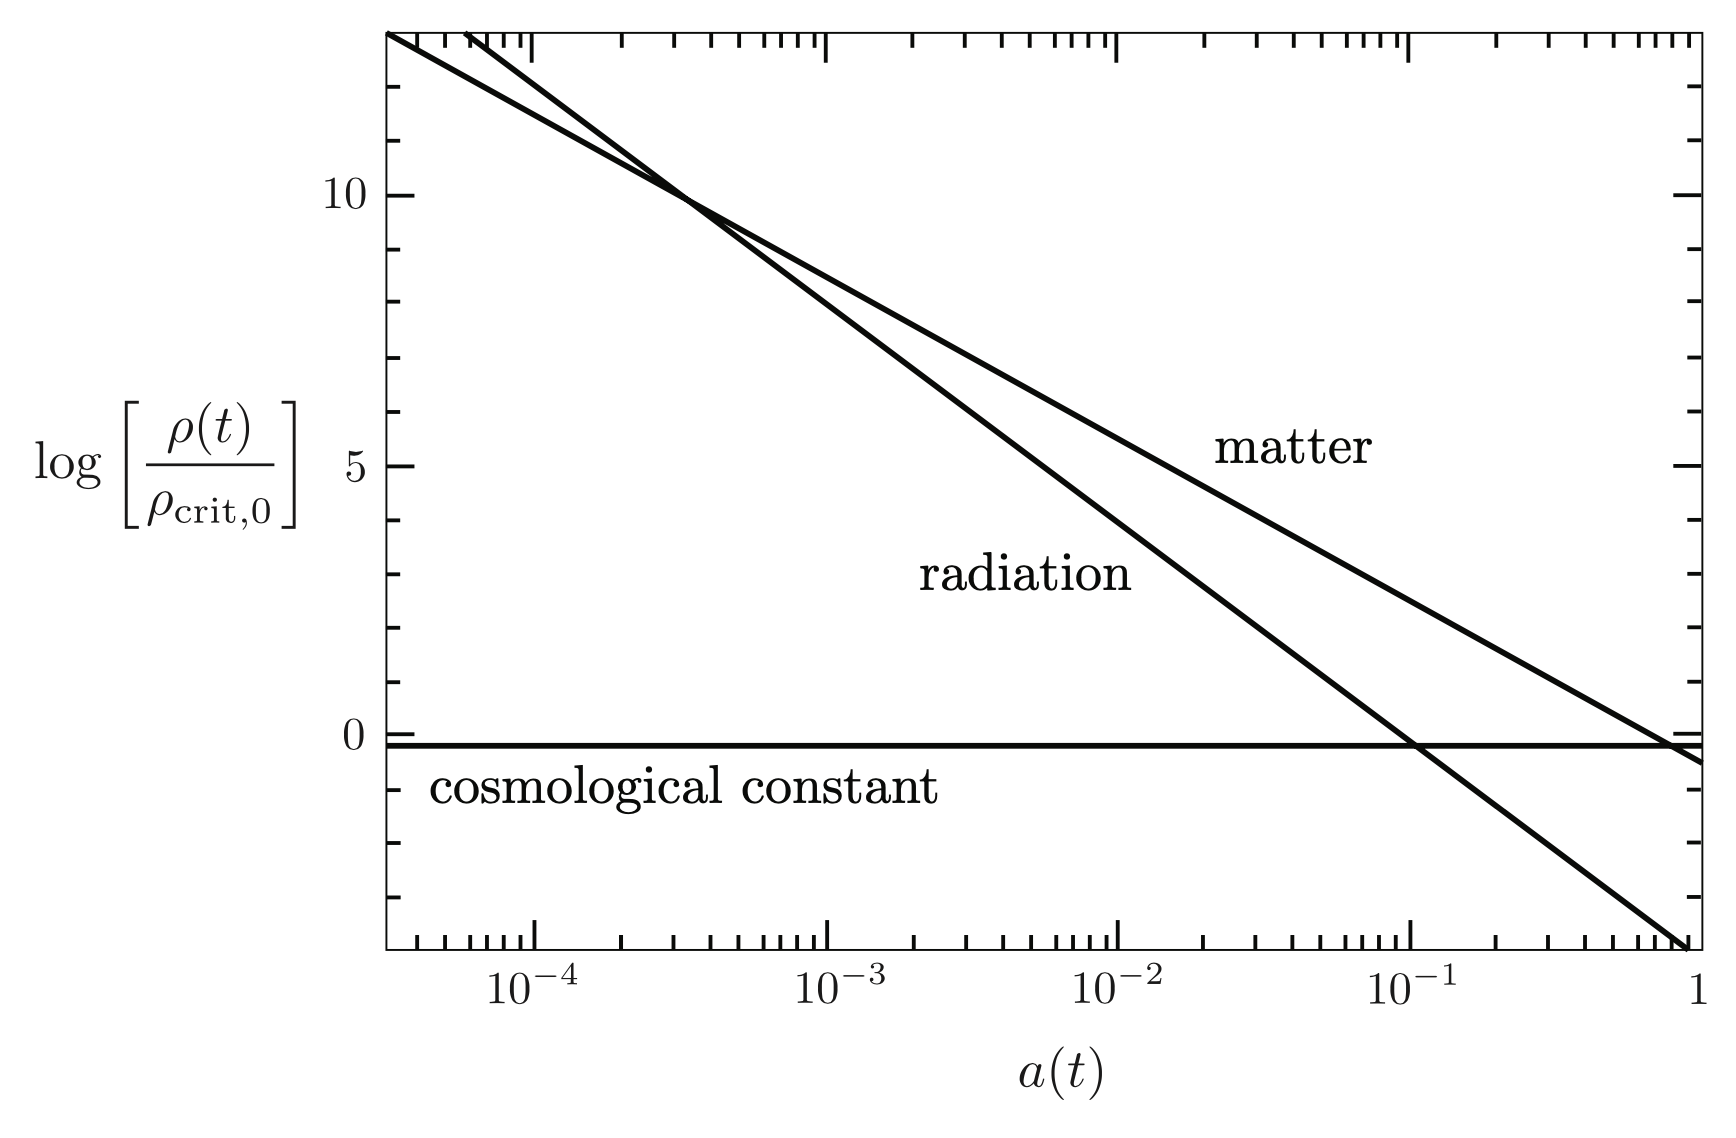
\includegraphics[width=0.95\textwidth]{figures/darkmatter/cosmology.png}
    \caption{Evolution of the energy densities in the universe. Figure reproduced from Ref.~\cite{Baumann2018}.}
    \label{fig:darkmatter:cosmology:energydensity}
\end{figure}


\section{Dark matter relic density}
\label{sec:dm:production}
The early universe was sufficiently hot and dense for dark matter \(\chi\) and other particle species \(f\) to be in thermal equilibrium. Reactions \(\chi \overline{\chi} \leftrightarrow f \overline{f}\) took place with the interaction rate
\begin{align}
    \Gamma = n \langle \sigma v \rangle,
\end{align}
where \(n\) denotes the particle number density and \(\langle\sigma v\rangle\) denotes the thermally averaged product of the interaction cross-section and the average velocity of the particles.
The expansion of the universe decreases the particle number density, until at some point it drops to a point at which interactions hardly occur and dark matter decouples from other particles. The point, at which the interaction rate \(\Gamma|_{T_{\text{dec}}}\) drops below the Hubble expansion \(H|_{T_{\text{dec}}}\), is defined by the decoupling temperature \(T_{\text{dec}}\). This process is referred to \emph{freeze-out} because the dark matter particle number density approaches a constant value for \(T < T_{\text{dec}}\). This constant value is the dark matter relic density.

The dark matter relic density can be derived by solving the Boltzmann equation
\begin{align}
    \frac{\dd{n}}{\dd{t}} = \langle \sigma_{\text{ann}} v \rangle (n_{\text{eq}}^2 - n^2)- 3 H n,
    \label{eq:dm:production:boltzmann}
\end{align}
where \(n_{\text{eq}}\) denotes the particle number density in equilibrium, \(H\) denotes the Hubble constant and \(\langle \sigma_{\text{ann}} v \rangle\) denotes the thermally averaged product of the annihilation cross-section and the velocity of the annihilating particles.

The Boltzmann equation is solved numerically under the condition of constant entropy. The dark matter relic density density in terms of the density parameter and the reduced Hubble constant \(h = H_{0} / \SI{100}{\kilo\meter\per\second\per\mega\parsec} \approx 0.7\) can be approximated as
\begin{align}
    \Omega_{X} h^2 \approx \frac{\SI{3e-27}{\cubic\centi\meter\per\second}}{\langle \sigma_{\text{ann}} v \rangle}.
\end{align}
The dark matter relic density is determined by the annihilation cross-section at the time of the freeze-out.
\Cref{fig:darkmatter:relicabundance:relicabundance} shows the dark matter particle number density as a function of the dimensionless parameter \(x = m_{\chi} / T\). The dotted line corresponds to the evolution of the number density for dark matter remaining in equilibrium without occurrence of any freeze-out. The number density decreases exponentially as a function of \(x\) until the interaction rate becomes too small for dark matter particles to remain in thermal equilibrium, resulting in a constant number density \(N_{X}^{\infty}\) determined by the point of freeze-out \(x_{F} = m_{\chi} / T_{\text{dec}}\). The strength of the interaction defines the dark matter relic density: a large dark matter annihilation cross-section corresponds to a smaller relic density.

\begin{figure}[htbp]
    \centering
    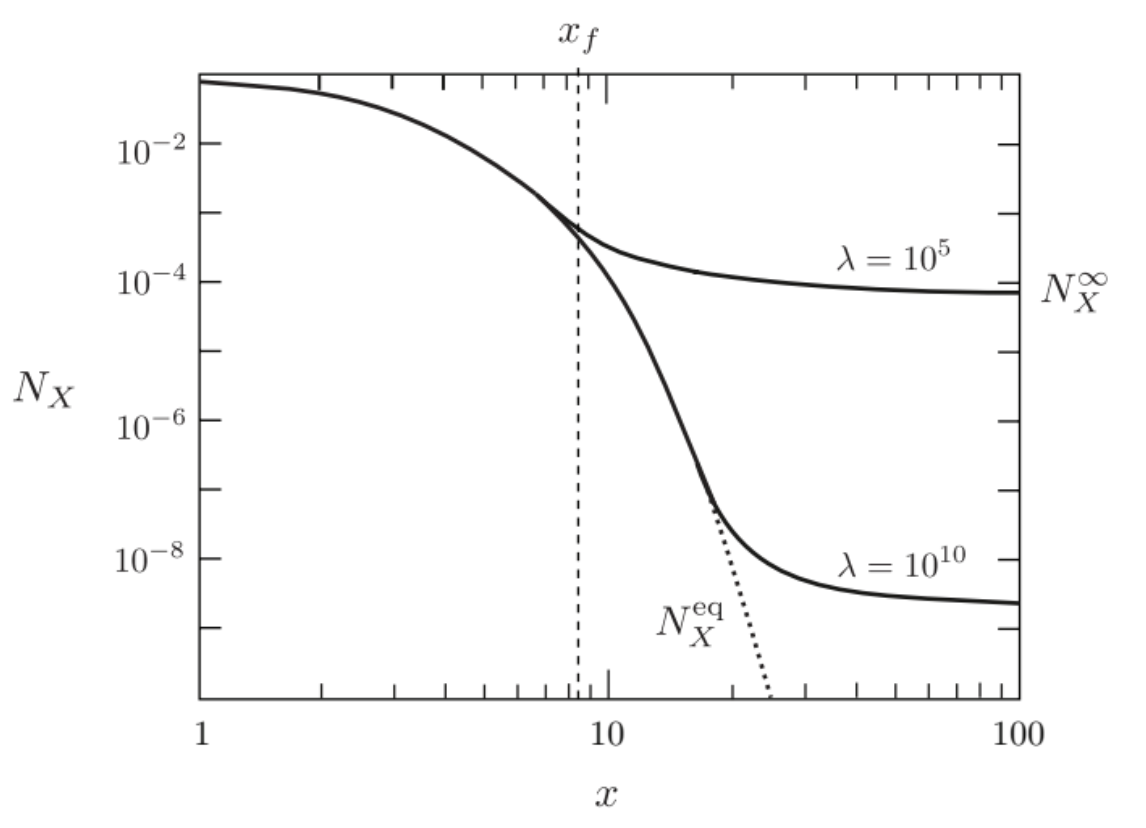
\includegraphics[width=0.9\textwidth]{figures/darkmatter/relicdensity.png}
    \caption{Abundance of dark matter particles \(N_{X}\) in dependence of the dimensionless parameter \(x = m_{\chi} / T\). The freeze-out occurs at the point, where the temperature \(T\) drops below the dark matter particle mass \(m_{\chi}\). The annihilation cross-section is expressed as \(\lambda = \frac{2 \pi^2}{45} g^{\star} \frac{m_{\chi} \langle \sigma_{\text{ann}} v \rangle}{H(m_{\chi})}\), where \(g_{S\star}\) denotes the effective number of degrees of freedom in entropy. Figure reproduced from Ref.~\cite{Baumann2018}.}
    \label{fig:darkmatter:relicabundance:relicabundance}
\end{figure}

For typical weak interaction cross-sections of the order \(\mathcal{O}(\sigma) = \SI{1}{\pico\barn}\) and for a dark matter particle with its mass at the electroweak scale, the observed dark matter relic density \(\Omega_{\chi} h^2 = 0.1188\) is obtained. This striking coincidence is known as the ``WIMP miracle'', referring to the dark matter particle candidate being a weakly interacting massive particle (WIMP).

The simplified calculation discussed here neglects several aspects, which can lead to significant changes in the relic density. It has been shown that the presence of a scalar field in the early universe could modify the value of the relic density. If the dark matter particle mass is similar to other particles, which share a quantum number with the dark matter particle, or if there are several different dark matter particles, co-annihilations occur. In this case, the first term in \Cref{eq:dm:production:boltzmann} needs to account for interactions among the different species, typically resulting in a much more efficient annihilation of dark matter. Radiative corrections in resonant Sommerfeld enhancement are another effect, which can cause dramatic changes in the relic density.


\section{Evidence for dark matter}
\label{sec:dm:evidence}
There is compelling evidence for the existence of dark matter on all astrophysical scales, including rotation curves of gas and stars in galaxies, large samples of galaxy clusters, strong and weak gravitational lensing, distant supernovae, studies of the cosmic microwave background, and large structure formation.

\subsection{Galactic scale}
\label{sec:dm:evidence:galaxy}
The first evidence for the existence of dark matter on sub-galactic scales comes from observations of the Dutch astronomer Jan Oort in 1932. He studied the motion of the stars in our galactic neighbourhood and measured the velocity of stars near the galactic plane by studying their Doppler shifts. His observations found them moving faster than expected --- even so fast that they should be able to escape the gravitational pull of the luminous mass in the Milky Way. Consequentially, he postulated that there must be more galactic mass present to keep the stars on their Keplerian orbits.

The strongest evidence for dark matter on galactic scales is based on the observation of the rotation curves of galaxies. These rotation curves are graphs of the circular velocities of the galaxy's constituents (stars and gas) as a function of their distance from the galactic centre.
\Cref{fig:darkmatter-rotationcurve} shows the rotation curve of the NGC 6503 galaxy.
\begin{figure}[htbp]
    \centering
    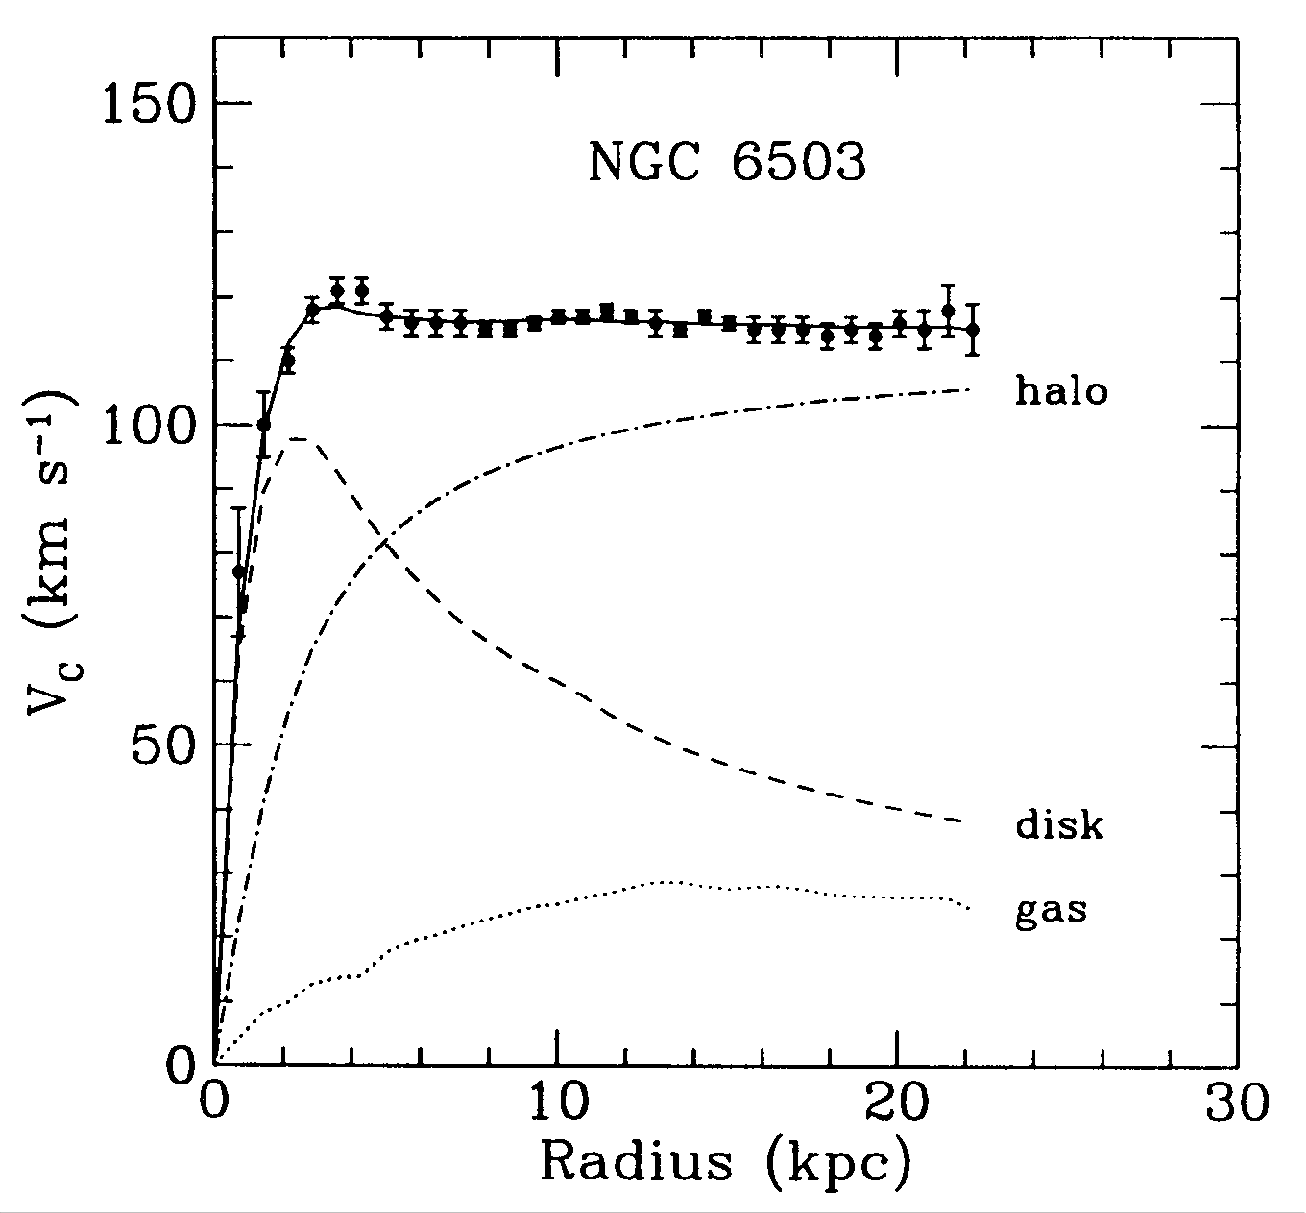
\includegraphics[width=0.95\textwidth]{figures/darkmatter/rotationcurve.png}
    \caption{Galactic rotation curve for NGC 6503 (observed data taken from Ref.~\cite{Burbidge1964}). The decomposition of the rotation curve in contributions from disk and gas potentials shows that an additional contribution due to the dark matter halo is required to match the data. Figure reproduced from Ref.~\cite{Freese2008}.}
    \label{fig:darkmatter-rotationcurve}
\end{figure}
The most striking feature is that the rotation curve approaches a flat shape at large distances, even beyond the edge of the visible disk. The circular velocity of an object on a stable Keplerian orbit is expected to be
\begin{align}
    v(r) = \sqrt{\frac{G M(r)}{r}} = \sqrt{4 \pi G \frac{\int \rho(r) r^2 \dd{r}}{r}},
\end{align}
where \(\rho(r)\) is the mass density profile. Beyond the edge of the visible disk, the rotation curve should be falling proportional to \(1 / \sqrt{r}\). The observation of an approximately constant distribution for large distances implies the existence of a dark matter halo with a mass density profile approaching \(\rho = 1 / r^2\) for large distances. The dark matter halo is expected to fall off faster at some point to keep the total mass of the galaxy finite.

Although there is consensus about the shape of dark matter haloes in the large-distance-limit, the predicted shape in the innermost region of the halo is subject of contention. Cosmological N-body simulations predict dark matter halos with density increasing steeply at small distances (``cusps''). The observed rotation curves of most dwarf galaxies, however, suggest flat, central dark matter density profiles (``cores''). This ``cusp-core problem'' is subject of ongoing investigation.

The velocity dispersion of dwarf spheroidal galaxies (dSphs), small satellite galaxies mostly within \SI{300}{\kilo\parsec} of the Milky Way, is another hint for the existence of dark matter~\cite{Strigari2018}. Dwarf spheroidal galaxies are the nearest, smallest and least luminous galaxies observed to date. They are among the galaxies most strongly dominated by dark matter~\cite{Walker2013}.

Further evidence on galactic scales comes from weak gravitational lensing of distant galaxies by foreground structures~\cite{Bartelmann2016}. Light originating from a luminous source is deflected by a large amount of matter between the source and the observer. The resulting image distortion is known as gravitational lensing and enables the determination of the mass of the foreground structure. Weak gravitational lensing data can provide constraints on the extent and shapes of the galactic dark matter halos~\cite{Hoekstra2002} and gives strong constraints on alternative theories of gravity.


\subsection{Galaxy cluster scale}
\label{sec:dm:evidence:cluster}
The investigation of the velocity dispersion of galaxies in the Coma cluster by Fritz Zwicky arguably pioneered the field of dark matter. Zwicky studied the Doppler-shift of several galaxies in a data set published by Edwin Hubble and Milton Humason and noticed at least eight galaxies with an apparent velocity exceeding \SI{6000}{\kilo\meter\per\second}. For these galaxies to be gravitationally bound, the galaxy cluster is required to have a sufficiently large gravitational potential. Using the virial theorem, he inferred the mass density of the Coma cluster. The estimate for the total mass of the cluster is
\begin{align}
    m_{\text{cluster}} = \sum_{i} m_{\text{galaxy}, i} \approx \frac{2 \langle v^2 \rangle}{G \langle 1 / r\rangle},
\end{align}
where \(\langle v^2 \rangle\) is the average velocity of galaxies in the cluster and \(\langle 1 / r \rangle\) is the average inverse distance between galaxies. Another way to estimate the total mass of the cluster is to measure its luminosity. Comparing the two estimates, he found the estimate based on the cluster's gravitational potential to be 400 times larger than that derived from observations of luminous matter.
Zwicky's use of the phrase ``dunkle (kalte) Materie'' is typically regarded as the first use of the term ``dark matter'' and established the convention of including the photograph of Fritz Zwicky making a silly face in public talks on dark matter.

Zwicky also pioneered the idea that entire galaxy clusters could act as gravitational lenses~\cite{Zwicky1937}. Weak gravitational lensing provides accurate estimates of the total mass of galaxy clusters and thereby provides evidence for the existence of dark matter.
In strong gravitational lensing~\cite{Bartelmann2010}, the light-bending effect is even strong enough to produce multiple images or arcs of the source. If the source, the observer and the matter in between (also called the ``lens'') are aligned, the source is observed in the form of an Einstein ring~\cite{Einstein1936}. The ring's angular radius \(\theta_{E}\) allows estimating the mass \(M\) of the lens via
\begin{align}
    \theta_{E} = \sqrt{4 G M \frac{d_{LS}}{d_{L} d_{S}}},
\end{align}
where \(G\) denotes Newton's constant, \(d_{L}\) denotes the distance to the lens, \(d_{LS}\) denotes the distance between source and lens and \(d_{S}\) denotes the distance to the source.

\Cref{fig:dm:evidence:cluster:abell2218} shows an image of the Abell 2218 galaxy cluster, an exceptionally rich lensing cluster at redshift \(z=0.175\). The galaxies lying behind the cluster's core are magnified and distorted into long arcs, some of them are even multiply imaged. The mass estimated from gravitational lensing exceeds the X-ray based estimate by at least a factor of 2.5~\cite{AbdelSalam1998}.
\begin{figure}[htbp]
    \centering
    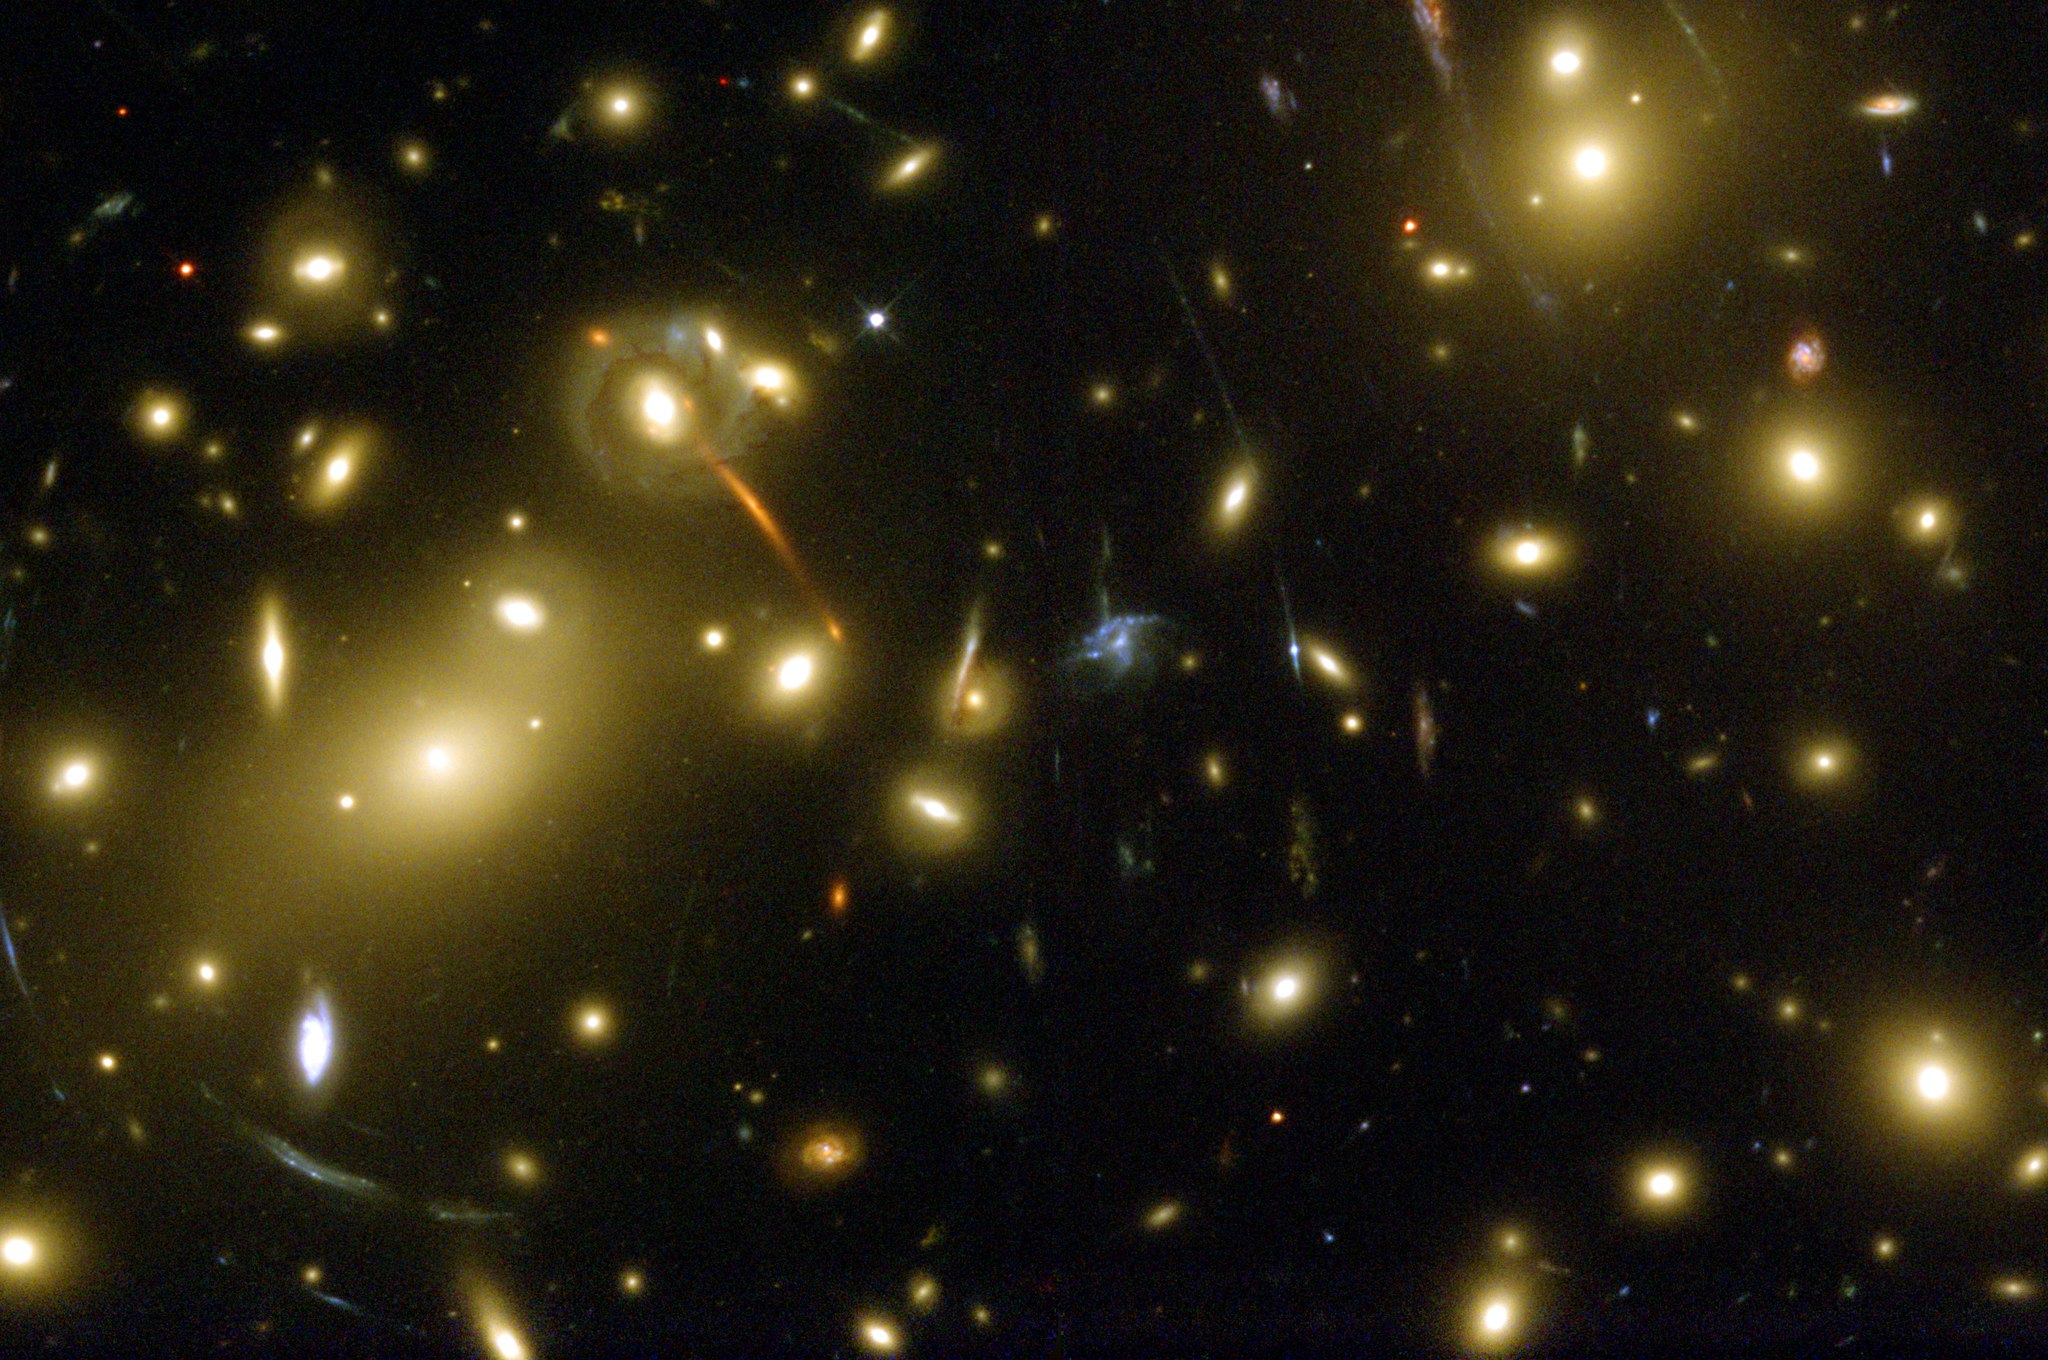
\includegraphics[width=0.95\textwidth]{figures/darkmatter/abell_NGC2218.jpg}
    \caption{Image of the galaxy cluster Abell 2218 and its gravitational lenses, taken by the Hubble space telescope in 1999. Image by Andrew Fruchter (STScI) et al., WFPC2, HST, NASA / Public domain.}
    \label{fig:dm:evidence:cluster:abell2218}
\end{figure}

Arguably the most dramatic evidence for dark matter is provided by observations of the galaxy cluster 1E\num{0657}-\num{558}~\cite{Tucker1998}, also known as ``bullet cluster''. It consists of two sub-clusters of galaxies, which are thought to have previously collided. \Cref{fig:dm:evidence:cluster:bullet} shows images of the bullet cluster from different sources, overlaid with the reconstructed cluster surface mass density \(\kappa\) obtained from weak gravitational lensing. The visible matter of the bullet cluster consists of clouds of hot gas (visible in the optical image), which constitute the majority of the cluster's baryonic matter, and stellar objects (visible in the X-ray image).

The stars are cleanly separated into two distinct sub-clusters, as the probability of individual galaxies colliding is small. In contrast, the clouds of hot gas have interacted ferociously, as the collision of the sub-clusters slowed the gas and left it displaced from the stars. Most of the matter of the sub-clusters, however, is dark matter, which is indicated by the distribution of the reconstructed cluster surface mass density \(\kappa\).

The dark matter in each of the two sub-clusters passed through, seemingly unaffected by the collision. These observations indicate that dark matter interacts weakly both with baryonic matter and with itself. The spatial offset of the centre of the total mass distribution from the centre of the baryonic mass distribution is highly significant (\(8\sigma\)) and gives strong constraints on alternative models of gravity.

\begin{figure}[htbp]
    \centering
    \begin{subfigure}{1.\textwidth}
      \centering
      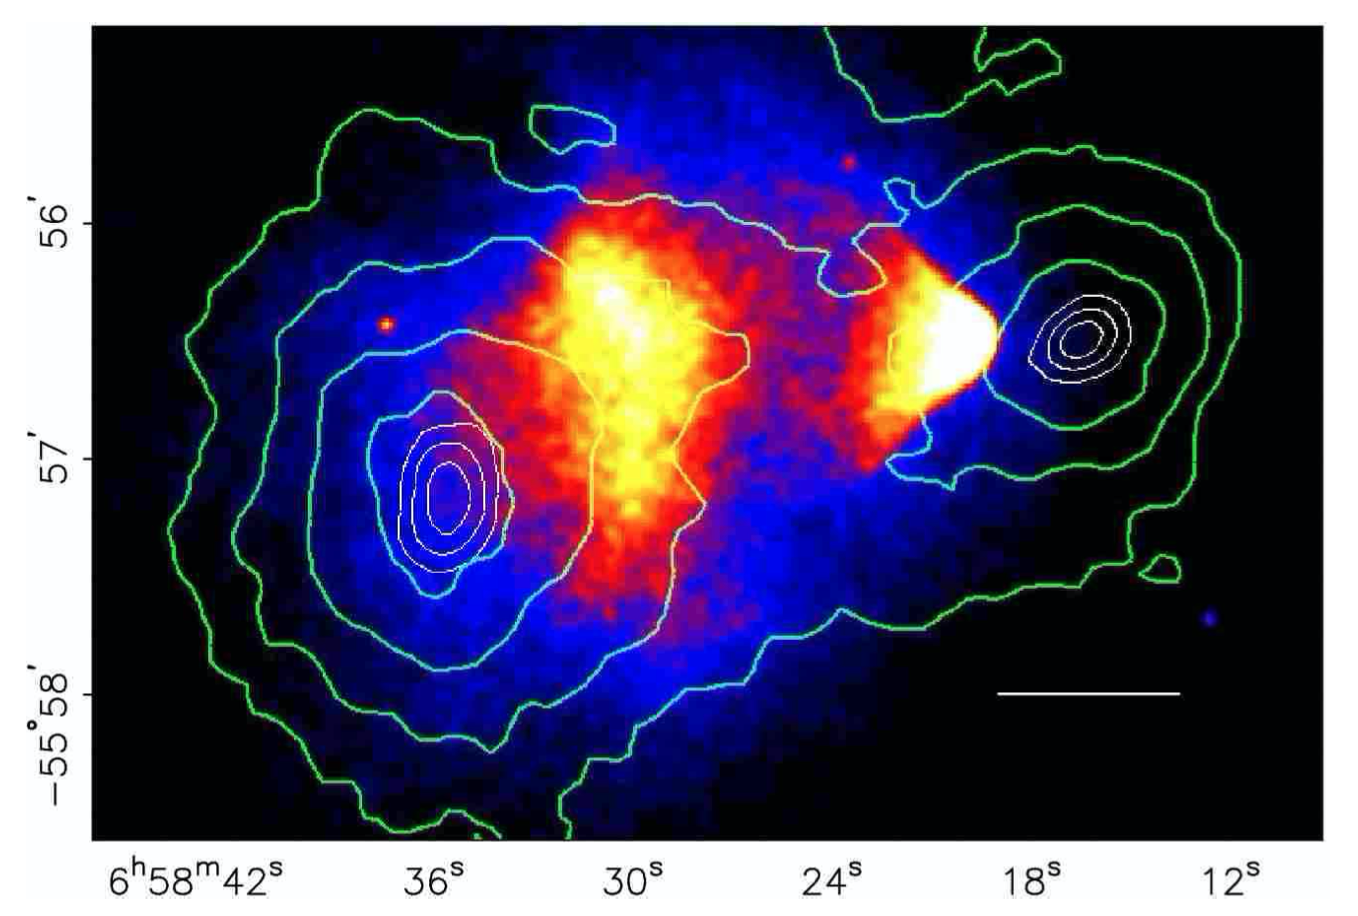
\includegraphics[width=0.95\textwidth]{figures/darkmatter/bulletcluster_magellan.png}
      \caption{Colour image of 1E\num{0657}-\num{558} from the \SI{6.5}{\meter} Magellan telescopes located at the Las Campanas observatory, Chile.}
      \label{fig:dm:evidence:cluster:bullet:magellan}
    \end{subfigure}
    \\
    \begin{subfigure}{1.\textwidth}
      \centering
      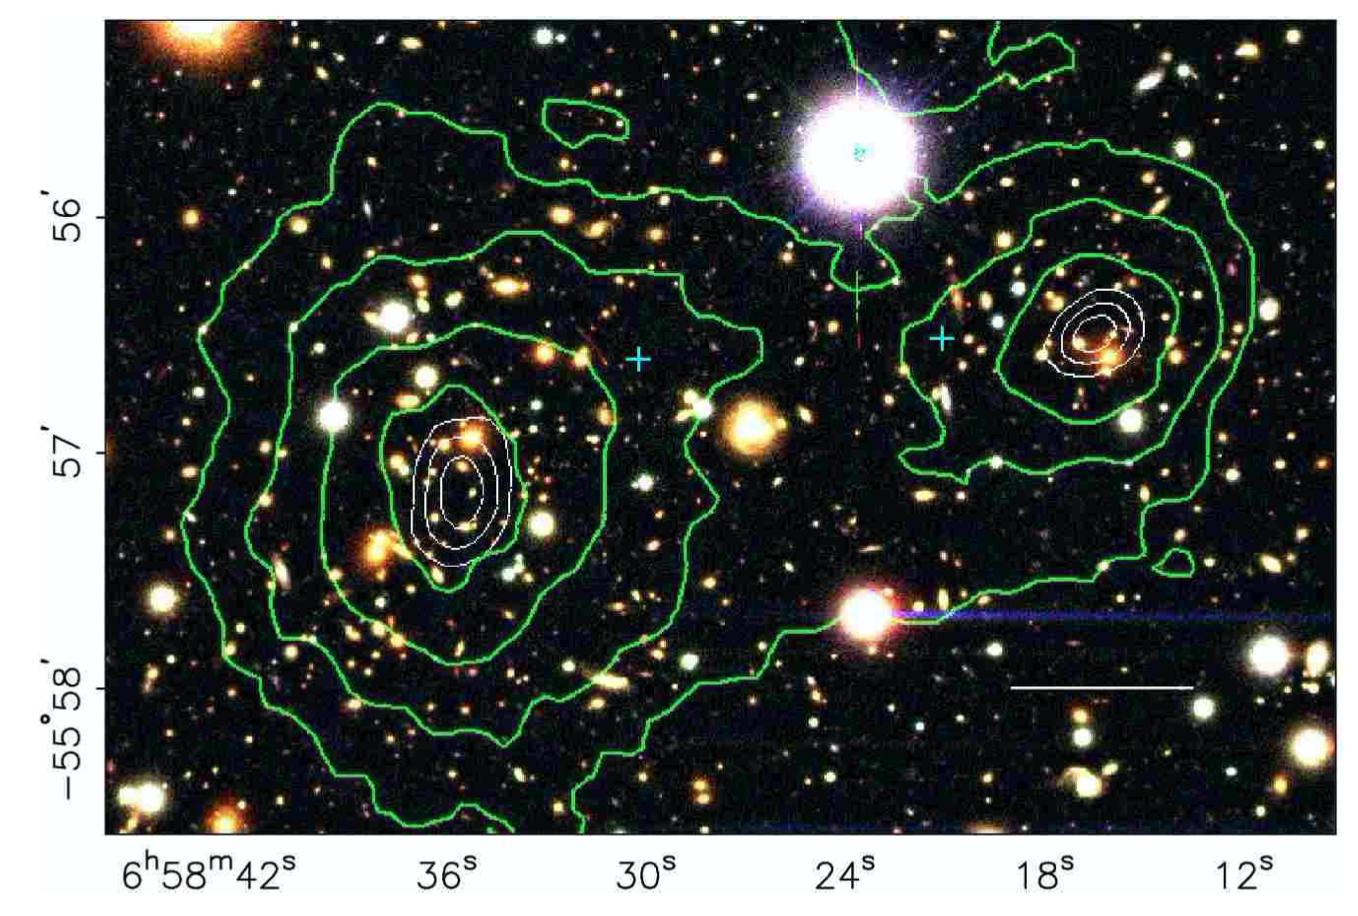
\includegraphics[width=.95\textwidth]{figures/darkmatter/bulletcluster_chandra.png}
      \caption{X-ray image of 1E\num{0657}-\num{558} from NASA Chandra satellite observatory.}
      \label{fig:dm:evidence:cluster:bullet:chandra}
    \end{subfigure}
    \caption{Images of 1E\num{0657}-\num{558} based on optical (top) and X-ray observations (bottom). The green contours of the reconstructed cluster surface mass density \(\kappa\) obtained from weak gravitational lensing are overlaid in both images. The three white contours show the uncertainty in the position of the two primary galaxy concentration centres, corresponding to \(1\sigma\), \(2\sigma\), and \(3\sigma\) confidence levels. Figures reproduced from Ref.~\cite{Clowe2006}.}
    \label{fig:dm:evidence:cluster:bullet}
\end{figure}


\subsection{Cosmological scale}
\label{sec:dm:evidence:cosmology}
Although the evidence on the scales of galaxies and galaxy clusters for themselves is compelling, the observations do not allow for an estimate of the total amount of dark matter in the universe. This information can be extracted from the analysis of cosmic microwave background data.

The cosmic microwave background (CMB), which was discovered in 1965 by Arno Penzias and Robert Wilson~\cite{Penzias1965}, is electromagnetic radiation with a black body radiation spectrum at temperature \(T_{\text{CMB}} = \SI{2.72548 \pm 0.00057}{\kelvin}\)~\cite{Fixsen2009}. It consists of primordial photons created in the early universe, which were in thermal equilibrium (c.f. the discussion for dark matter particles in \Cref{sec:dm:production}). Photons and free electrons frequently interacted via scattering processes, as space was filled by a charged plasma. The interaction rate decreased when the electrons combined with protons to form electrically neutral hydrogen atoms. Consequentially, the photons decoupled and could propagate undisturbed. The CMB can be thought of as the sphere of the last scattering with the observer in the centre and allows probing the conditions in the early universe directly.

In the last three decades, the CMB has been mapped by experiments with increasing precision~\cite{Smoot1992,Bennett2003,Spergel2003,Spergel2007,Reichardt2009,Planck2019,Planck2020}. The almost uniform temperature of the CMB suggests a phase of rapid, inflationary expansion of the universe, which is driven by the cosmological constant \(\Lambda\).
After subtracting the dipole moment associated with the movement of the earth, the CMB exhibits temperature fluctuations with the characteristic scale \(\delta T / T_{\text{CMB}} \approx 10^{-5}\). These tiny fluctuations are used to determine the cosmological parameters. The temperature fluctuations are parametrised as an expansion in spherical harmonics \(Y_{lm}(\theta, \varphi)\)\footnote{The base mode \(l=0\) corresponds to the CMB temperature \(T_{\text{CMB}}\). The first mode \(l=1\) corresponds to the dipole anisotropy. Therefore, the expansion in the fluctuations starts at \(l=2\).}
\begin{align}
    \frac{\delta T}{T_{\text{CMB}}} (\theta, \varphi) &= \sum_{l=2}^{\infty} \sum_{m=-l}^{l} a_{lm} Y_{lm}(\theta, \varphi).
\end{align}

Assuming the values of the coefficients \(a_{lm}\) are independent of the index \(m\), it is possible to define the observed angular power spectrum
\begin{align}
    C^{TT}_{l} = \frac{1}{2l+1} \sum_{m=-l}^{l} \abs{a_{lm}}^2
\end{align}
for discrete values of the multi-pole moment \(l \propto \pi / \phi\). The CMB map and the power spectrum measured by PLANCK~\cite{Planck2019} is shown in \Cref{fig:dm:evidence:cosmology:cmb}.

\begin{figure}[htbp]
    \centering
    \begin{subfigure}{1.\textwidth}
      \centering
      \includegraphics[width=0.95\textwidth]{figures/darkmatter/cmb_planck_map.png}
      \caption{CMB sky map. The grey line delineates a region, which lies mostly around the Galactic plane, where residuals from foreground emission are expected to be substantial and which is therefore masked in the analysis.}
      \label{fig:dm:evidence:cosmology:cmb:map}
    \end{subfigure}
    \\
    \begin{subfigure}{1.\textwidth}
      \centering
      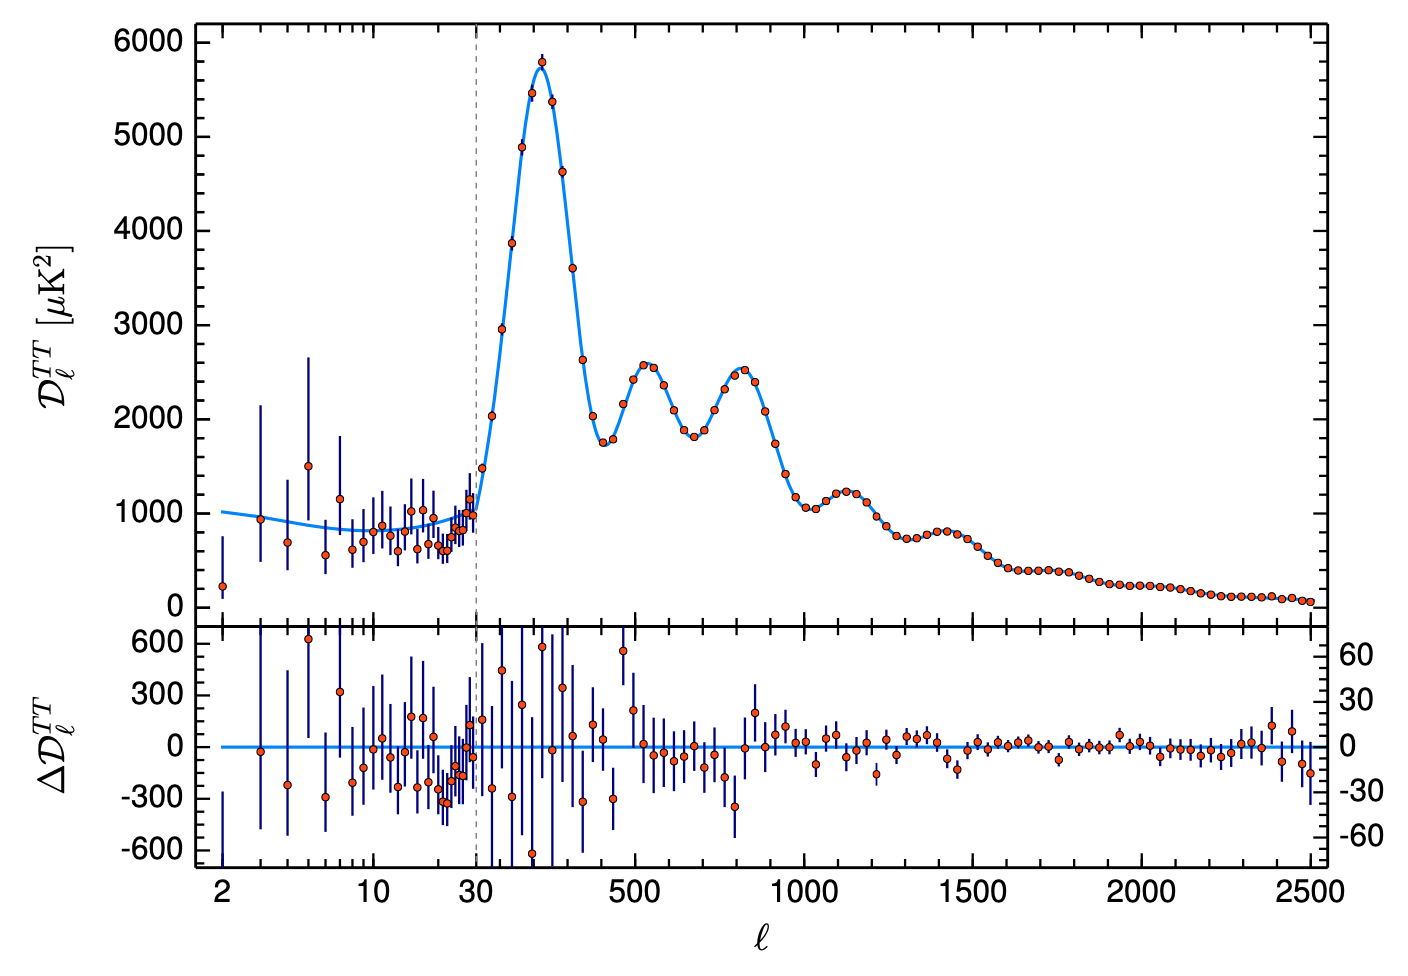
\includegraphics[width=.95\textwidth]{figures/darkmatter/cmb_planck_spectrum.png}
      \caption{CMB temperature power spectrum. The upper panel shows the scaled power spectrum modes \(D^{TT}_{l}= l(l+1) C^{TT}_{l} / (2\pi) \). The \(\Lambda\)-CDM model best fit to the data is overlaid in light blue in the upper panel. The residuals with respect to this model are shown in the lower panel. For better visualisation, the horizontal scale changes at \(l=30\) from a logarithmic scale to a linear scale.}
      \label{fig:dm:evidence:cosmology:cmb:spectrum}
    \end{subfigure}
    \caption{Planck (2018) observations of the CMB. Figures reproduced from Refs.~\cite{Planck2019} (top) and \cite{Planck2020} (bottom).}
    \label{fig:dm:evidence:cosmology:cmb}
\end{figure}

The measured power spectrum consists of a set of peaks, which each define an angular scale with particularly large contributions to the temperature fluctuations. The cosmological parameters can be inferred from a fit of the positions, shapes and relative sizes of the peaks in the spectrum. The peaks originate from acoustic waves in the baryon-photon fluid before the photon decoupling. These acoustic waves can be understood as the competing effects of gravity and radiative pressure. The baryon-photon fluid gets pulled into gravitational wells around regions of considerable matter accumulation. As more baryonic matter accumulates, the increasing photon pressure acts against the gravitational potential of the wells.

Even-numbered peaks are associated with the compression of the baryon-photon fluid due to gravity, whereas odd-numbered peaks are associated with the counteracting effect of radiative pressure. A higher baryon content in the baryon-photon fluid corresponds to smaller radiative pressure and larger compression peaks. Therefore, the relative amplitude between odd- and even-numbered peaks is a measure of the baryon density parameter \(\Omega_{b}\). Dark matter only contributes to the gravitational wells and does not respond to radiative pressure. The size of the third peak indicates a sizeable dark matter component at the time of the last scattering. The first peak corresponds to waves, which have only compressed once. Its position is used to determine the spatial curvature parameter \(\kappa\).

The estimates for the products of the cosmological density parameters and reduced Hubble constant \(h\)~\cite{Planck2020} are
\begin{itemize}
    \item baryon density parameter \(\Omega_{b} h^2 = \num{0.02237} \pm \num{0.00015}\)
    \item dark matter (DM) density parameter \(\Omega_{\text{DM}} h^2 = \num{0.1200} \pm \num{0.0012}\).
\end{itemize}
The estimates are compatible with the predictions from Big Bang nucleosynthesis~\cite{Simha2008} and with those obtained from the Sloan Digital Sky Survey~\cite{Tegmark2004}.

A global fit of the \(\Lambda\)-CDM model allows constraining the amount of dark energy by extracting the
\begin{itemize}
    \item cosmological constant density parameter \(\Omega_{\Lambda} = \num{0.6847} \pm \num{0.0073}\).
\end{itemize}
The knowledge of these fundamental cosmological parameters allows for a breakdown of the present composition of the universe in \SI{4.9}{\percent} baryonic matter, \SI{26.8}{\percent} dark matter and \SI{68.3}{\percent} dark energy.

The current structure of the universe is a result of the initial matter fluctuations in the early universe.
The temperature fluctuations in the CMB indicate that the early universe was not entirely homogeneous and isotropic. These density fluctuations have grown into the galaxies and galaxy clusters observed today. However, this could not have been achieved by baryonic matter alone.

Structure formation could only have occurred after the universe cooled down sufficiently for the photons to decouple. Then, however, there would not have been sufficient time to form the amount of structure observed today. Dark matter, on the other hand, is thought to decouple from the photons much earlier. Its density perturbations can form the gravitational wells acting as a seed for the gravitational collapse of visible matter. The observed large scale structure of the universe is compatible with the cold dark matter hypothesis~\cite{Blumenthal1984}.


\section{Candidates for dark matter particles}
\label{sec:dm:candidates}
It would be an understatement to say that several compelling candidates for dark matter have been proposed. The parameter space of dark matter models is vast and covers at least \num{30} orders of magnitude in the mass and \num{40} orders of magnitude in the interaction cross-section with protons~\cite{Ibarra2015}.

In analogy to the example of hidden planets in the Solar System in \Cref{sec:dm:intro}, one could naively assume dark matter to consist of yet unobserved baryonic matter.
Massive Astrophysical Compact Halo Objects (MACHOs)~\cite{Griest1993}, compact objects much less luminous but otherwise equivalent to ordinary stars, were among the first dark matter candidates. Possibilities for such objects include planets, brown dwarfs, neutron stars, Jupiter-like objects, and black holes. However, searches based on micro-lensing surveys and determinations of the cosmic baryon density from measurements of the primordial light element abundances and the CMB data strongly constrain the fraction of the dark matter constituted by MACHOs~\cite{Bertone2018}.

There are several compelling candidates for a non-baryonic dark matter particle. A suitable dark matter particle candidate must be able to be probed experimentally and needs to satisfy the following conditions~\cite{Taoso2008}:
\begin{enumerate}
    \item It has to be an electrically neutral,~\cite{McDermott2011} stable~\cite{Audren2014} particle with sufficiently low interactions to match the appropriate relic density~\cite{Srednicki1988}.
    \item It must lead to sufficiently low velocity during decoupling to allow for the observed large scale structure formation in the universe.
    \item It has to be compatible with the constraints
    \begin{itemize}
        \item on its self-interactions~\cite{Randall2008,Tulin2018},
        \item due to stellar evolution~\cite{Scott2009},
        \item from Big Bang nucleosynthesis~\cite{Kawasaki2015}
        \item from direct searches for dark matter~\cite{Liu2017},
        \item from indirect searches for dark matter~\cite{Conrad2017},
        \item from collider searches for dark matter~\cite{Buchmueller2017}, and
        \item due to other astrophysical observations.
    \end{itemize}
\end{enumerate}

A possible non-baryonic dark matter candidate in the SM appears to be the neutrino, as it has the ``undisputed virtue of being known to exist''~\cite{Bergstroem2000}. Neutrinos are neutral, have non-vanishing mass and only interact weakly with SM particles. They are an example of hot dark matter since they are still relativistic at the time of their decoupling due to their small mass \(m_{\nu} < \SI{1}{\electronvolt}\)~\cite{Aker2019}. However, neutrinos alone are not able to account for the total dark matter mass in the universe. The relic density parameter for neutrinos with mass \(\sum_{i} m_{\nu_{i}} = \SI{0.264}{\electronvolt}\) is predicted to be~\cite{Loureiro2019}
\begin{align}
    \Omega_{\nu} h^2 \approx \sum_{i} \frac{m_{\nu_{i}}}{\SI{92.5}{\electronvolt}} \lesssim 0.00285.
\end{align}
The relic density parameter is too small for neutrinos to be the dominant component of dark matter. Furthermore, the observed amount of structure in galaxy clustering is inconsistent with the predictions for a neutrino-dominated universe~\cite{White1984}.

These arguments prove that the SM does not contain a viable candidate for a dark matter particle. However, several extensions of the SM predict viable candidates:

\textbf{Sterile neutrinos}~\cite{Dodelson1994,Boyarsky2019} are right-handed (\(\text{SU}(2)_{L}\) singlet) neutrinos, which do not interact with SM particles except by small mixing \(\theta\) with left-handed \(\text{SU}(2)_{L}\)-active neutrinos. They can overcome the constraints which ruled out the SM neutrinos as dark matter. The mass of sterile neutrinos is expected to be in the \si{\kilo\electronvolt}-range. Although sterile neutrinos are expected to decay predominantly to three left-handed neutrinos, their radioactive decay mode to one left-handed neutrino and a photon gives rise to a quasi-monochromatic photon line at half the sterile neutrino-mass and can be exploited for searches.
%An overview of current constraints on thermally produced sterile neutrinos is shown in \Cref{fig:dm:candidates:constraints:sterile-neutrinos}.

\textbf{Axions} are very light pseudo-scalar bosons, which have been originally proposed as a solution to preserve \(CP\) symmetry in strong interactions~\cite{Peccei1977}. Axion-like-particles (ALPs) define a more general class of very light, weakly coupled  bosons, which are excellent candidates for particle dark matter in the ALP mass range \(\SI{e-6}{\electronvolt} < m_{A} < \SI{e-2}{\electronvolt}\)~\cite{Graham2015}. The main search strategy for axion searches is based on the axion-photon conversion in external magnetic fields.
%An overview of current constraints on axions is shown in \Cref{fig:dm:candidates:constraints:axions}.

% \begin{figure}[htbp]
%     \centering
%     \begin{subfigure}{.95\textwidth}
%       \centering
%       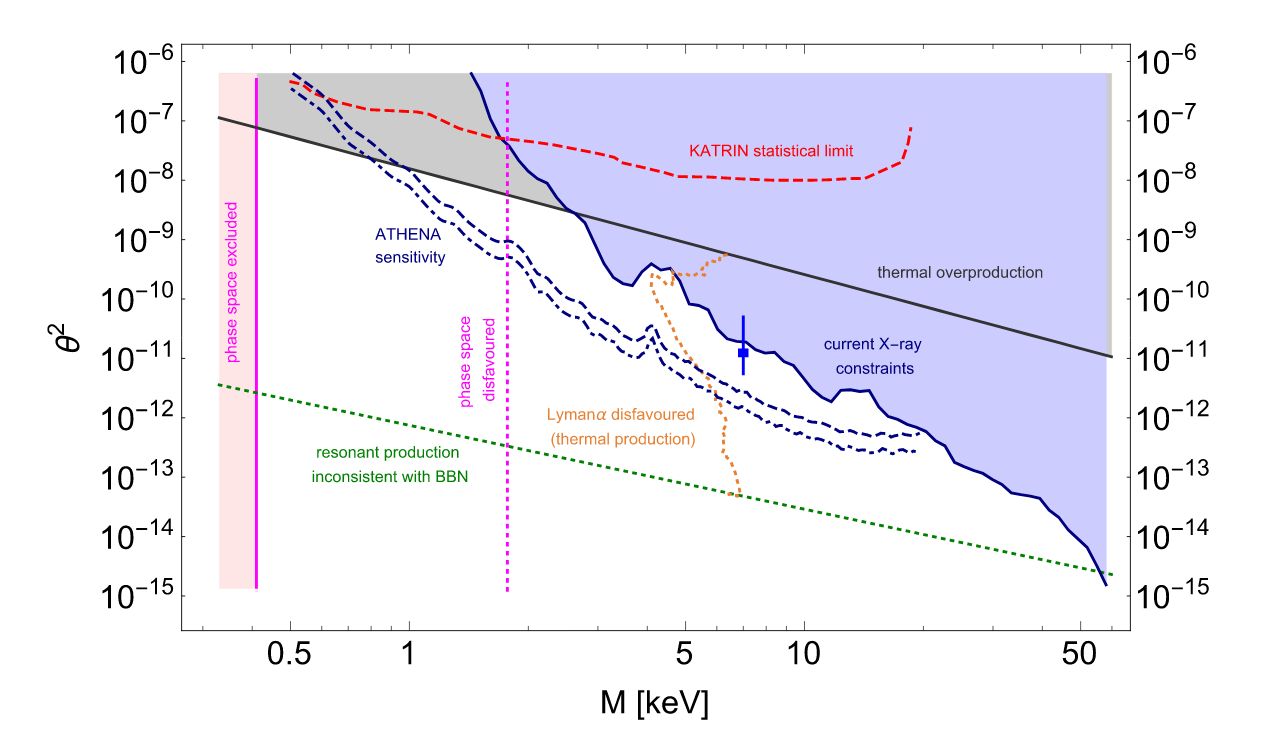
\includegraphics[width=1.\textwidth]{figures/darkmatter/sterile_neutrino.png}
%       \caption{Constraints on thermally produced sterile neutrinos in the plane defined by the sterile neutrino mass and the mixing \(\theta\) with SM neutrinos. The solid lines indicate largely model-independent constraints from phase-space considerations for fermionic dark matter in dSphs (pink), from current non-observations of X-rays from the decay of sterile neutrinos to photons and SM neutrinos (violet), and from the observed relic density (black). Further constraints originate from Big Bang nucleosynthesis (green) and structure formation (orange). The expected sensitivity improvements from the ATHENA X-ray telescope~\cite{Neronov2016} data is overlaid. Also, the expected sensitivity of the TRISTAN upgrade of the KATRIN experiment~\cite{Mertens2019} is indicated (red).}
%       \label{fig:dm:candidates:constraints:sterile-neutrinos}
%     \end{subfigure}
%     \\
%     \begin{subfigure}{1.\textwidth}
%       \centering
%       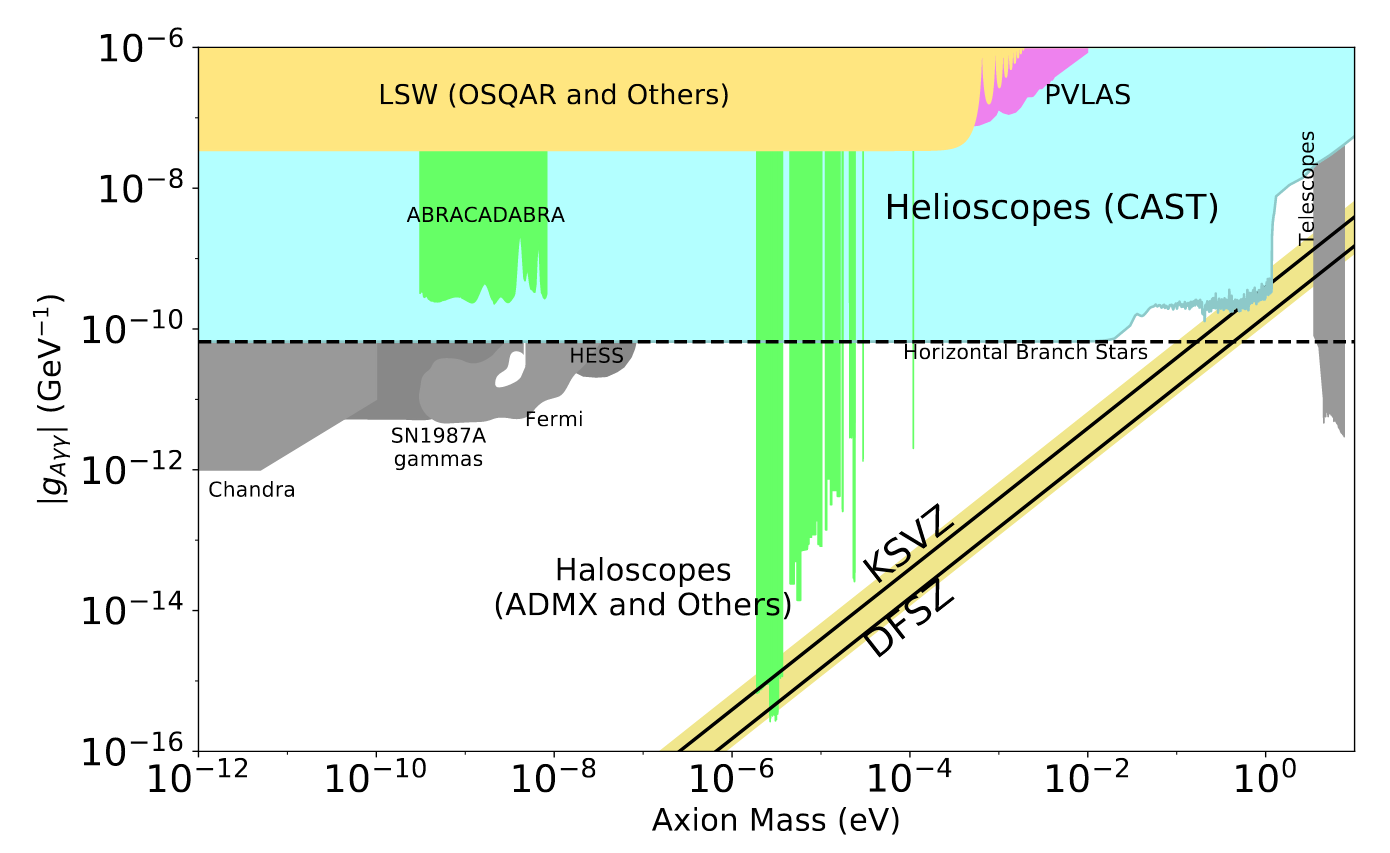
\includegraphics[width=.9\textwidth]{figures/darkmatter/axions.png}
%       \caption{Constraints on axions in the plane defined by the axion mass and the axion to two-photon coupling strength \(g_{A\gamma\gamma}\). The upper orange region is excluded by light-shining-through-wall (LSW) experiments, the purple region is excluded by searches for vacuum magnetic birefringence (PVLAS), the green regions are excluded by direct searches using haloscopes, the upper blue region is excluded by helioscope experiments searching for solar axions, and the light and dark grey regions are excluded by astrophysical observations. The diagonal yellow band indicates predictions of typical QCD axion models (KSVZ, DSFZ).}
%       \label{fig:dm:candidates:constraints:axions}
%     \end{subfigure}
%     \caption{Constraints on selected non-baryonic dark matter candidates. Figures reproduced from Refs.~\cite{Boyarsky2019} (top) and \cite{Tanabashi2018} (bottom).}
%     \label{fig:dm:candidates:constraints}
% \end{figure}

The \textbf{WIMP} paradigm (weakly interacting massive particle, denoted as \(\chi\)) defines a class of particularly well-motivated candidates for dark matter particles. WIMPs are neutral, stable or very long-lived particles. The interactions of WIMPs with the SM occur with similar strength as typical electroweak interactions. The WIMP mass is expected to range from \(\SI{10}{\giga\electronvolt} < m_{\chi} < \SI{100}{\tera\electronvolt}\)~\cite{Kolb1990,Griest1990}. Therefore, thermally produced WIMPs are non-relativistic by the time of decoupling and are a typical example of cold dark matter. Consequentially, the WIMP paradigm provides a simple mechanism to obtain the observed relic density, which is referred to as the ``WIMP miracle'' (c.f. \Cref{sec:dm:production}).
In regions of large WIMP density, they can annihilate and produce a flux of \(\gamma\)-rays, anti-particles and neutrinos. WIMP searches are discussed in detail in \Cref{sec:dm:searches}.

A notable example of a framework predicting WIMPs is the minimal supersymmetric extension of the SM (MSSM)~\cite{Fox2019}. In this model, the lightest supersymmetric particle (LSP), whose decay to SM particles is prohibited by a custodial symmetry, is a WIMP. Other theories predicting WIMPs include theories with extra-dimensions~\cite{Cheng2002} with Kaluza-Klein states, Little Higgs models~\cite{Birkedal2006} with the lightest \(T\)-odd particle, or technicolor theory~\cite{Kainulainen2007} with a massive fourth family neutrino, to name only a few.

The dark matter searches discussed in this dissertation focus on the WIMP paradigm.


\section{Search for WIMP dark matter}
\label{sec:dm:searches}
There are several complementary approaches to search for dark matter:
\begin{itemize}
    \item direct detection experiments measure the recoil of dark matter particles in the vicinity of the Earth on nuclei in the active detector material.
    \item indirect detection experiments search for an excess in the particle flux observed by earth-bound and satellite detectors due to pair annihilation of dark matter particles in regions of enhanced dark matter density.
    \item searches for dark matter at particle colliders investigate signatures of missing momentum in the detector plane transverse to the colliding beams due to dark matter pair production.
\end{itemize}
The experimental approaches for detecting the interactions of dark matter particles with SM particles are complementary. While direct and indirect detection experiments can establish the galactic origin of a signal, their sensitivity to the details of the interaction between dark matter and SM particles is limited. Collider searches, on the other hand, are unable to probe the lifetime of dark matter particles beyond the time scale required for traversing the detector but can probe their interactions in greater detail~\cite{Buchmueller2017}.
\Cref{fig:darkmatter:searches:overview} shows the relevant momentum ranges in the different kinds of searches with prototypical Feynman graphs.
\begin{figure}[htbp]
    \centering
    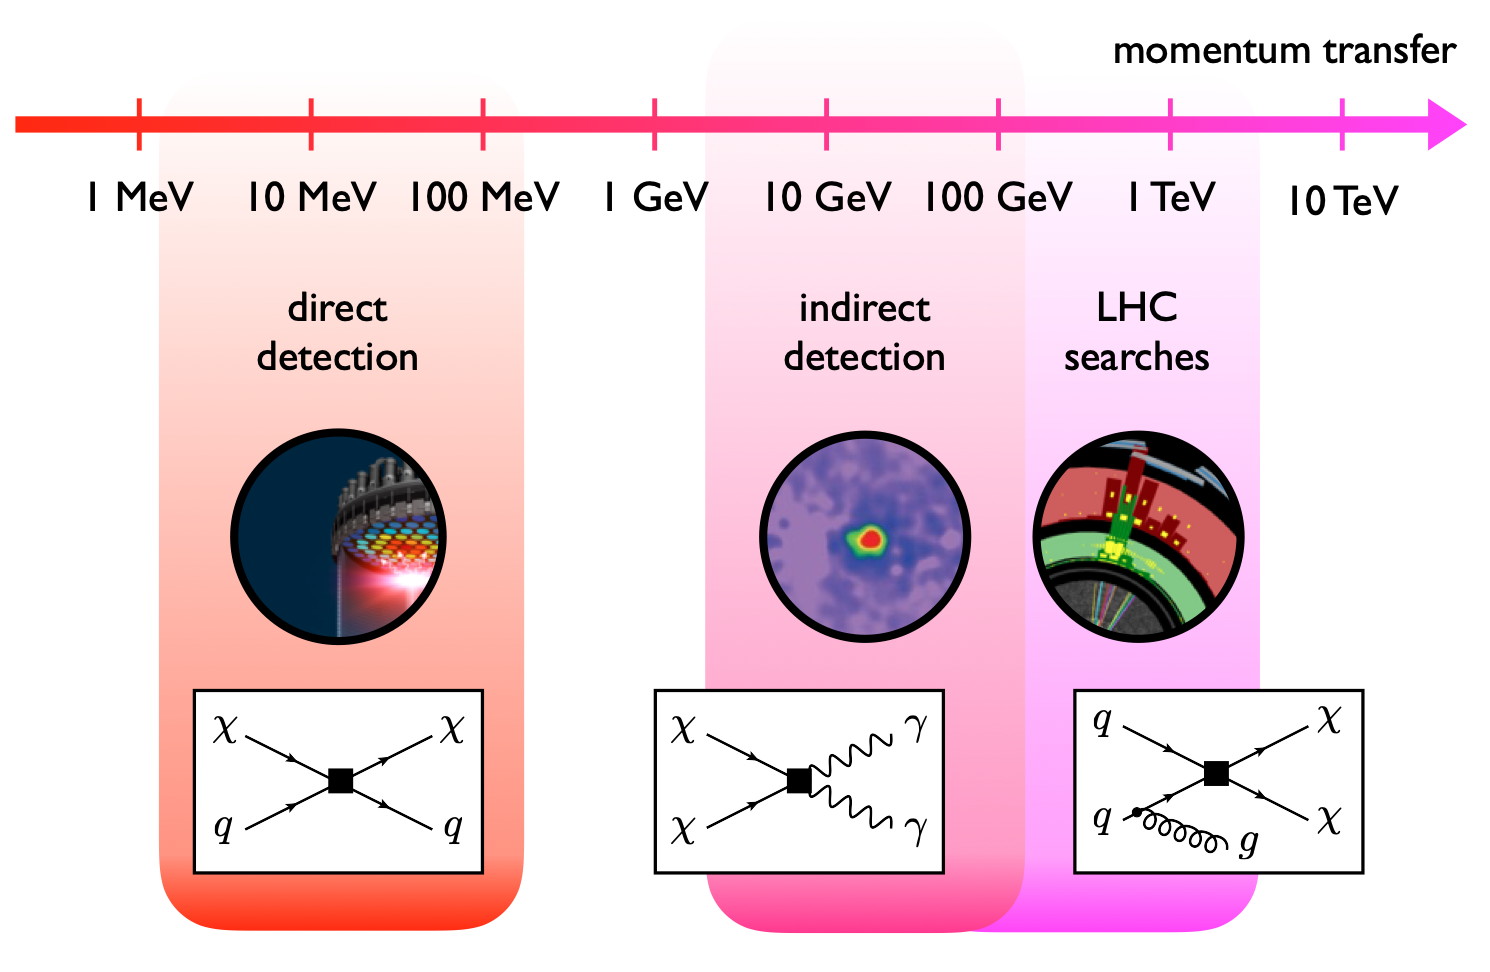
\includegraphics[width=0.9\textwidth]{figures/darkmatter/overview_searches.png}
    \caption{Range of momentum transfers probed by direct detection experiments, indirect detection experiments and collider searches with prototypical Feynman graphs illustrating the underlying processes. Figure reproduced from Ref.~\cite{Abe2020}.}
    \label{fig:darkmatter:searches:overview}
\end{figure}


\subsection{Direct detection experiments}
\label{sec:dm:searches:dd}
Direct detection experiments (c.f. Refs.~\cite{Liu2017,Schumann2019} for a review) aim to detect the nuclear recoil in the scattering of galactic WIMPs off target nuclei. The interaction rate of WIMPs with nuclei in the detector~\cite{Bertone2005}
\begin{align}
    R \approx \sum_{i} N_{i} n_{\chi} \langle \sigma_{i \chi} \rangle
\end{align}
depends on
\begin{itemize}
    \item the number of target nuclei \(N_{i} = m_{\text{detector}} / m_{A_{i}}\) in the active detector material for nucleons of species \(i\) with atomic weight \(A_{i}\),
    \item the local WIMP density \(n_{\chi} = \rho_{\chi} / m_{\chi}\), where \(\rho_{\chi}\) is the local WIMP energy density and \(m_{\chi}\) is the WIMP mass, and
    \item the cross-section \(\sigma_{i \chi}\) for interactions between WIMPs and nucleons of species \(i\), averaged over the relative WIMP velocity with respect to the detector.
\end{itemize}
The values of the astrophysical parameters are set to typical assumptions~\cite{Schumann2019} for the Solar System. The canonical value for the local WIMP energy density is \(\rho_{\chi} = \SI{0.3}{\giga\electronvolt\per\cubic\centi\meter}\). The WIMP velocity distribution \(f(\vec{v})\) is defined by the mean WIMP velocity \(v_{c} \approx \SI{220}{\kilo\meter\per\second}\) at the solar distance from the galactic centre and by the galactic escape velocity \(v_{\text{esc}} \approx \SI{544}{\kilo\meter\per\second}\), which determines the truncation of \(f(\vec{v})\).
The remaining free parameters are the WIMP mass \(m_{\chi}\) and the WIMP-nucleon interaction cross-section. The exclusion limits obtained from the non-observation of WIMP signals are usually shown as contours in the plane defined by these two parameters.

The primary signal in direct detection experiments are nuclear recoils. For WIMPs with mass in the range \(\SI{1}{\giga\electronvolt} < m_{\chi} < \SI{1}{\tera\electronvolt}\), the typical elastic recoil energy of the atomic nucleus ranges from \(\SI{1}{\kilo\electronvolt} < E_{\text{recoil}} < \SI{100}{\kilo\electronvolt}\). Electron recoil events can also be investigated, although their typical recoil energy is smaller.

The nuclear recoil energy can be converted into
\begin{itemize}
    \item thermal motion (phonons),
    \item ionisation (electrons) of the detector material,
    \item scintillation light (photons) through the Coulomb field of the charged nucleus.
\end{itemize}
These modes define the different detection channels of direct detection experiments. Typically, two channels are combined to achieve more powerful discrimination against electron recoil backgrounds from radioactivity.

Direct detection experiments require a very low background environment because of the meagre interaction rates for WIMP-nucleon interactions. Therefore, direct detection experiments are hosted in deep underground laboratories to suppress background produced by cosmic rays. Also, they employ passive shielding and active vetoes to suppress external backgrounds and are made of high-purity detector components to minimise internal backgrounds.
As the experiments increase their sensitivity to lower recoil energies, an irreducible background from the scattering of atmospheric and solar neutrinos becomes an issue. This background is referred to as the ``neutrino floor'' and poses new challenges to the future generation of experiments.

WIMP-nucleon scattering can be classified depending on the type of WIMP-nucleon coupling in
\begin{itemize}
    \item spin-independent (SI) interactions, which are mediated by scalar or vector couplings, with coherent and elastic WIMP scattering off all nucleons in the nucleus, and
    \item spin-dependent (SD) interactions, which are mediated by axial-vector couplings, with a \(J(J+1)\) dependence of the cross-section on the nuclear spin \(J\).
\end{itemize}
SI interactions give a larger signal than SD interactions because of the coherent scattering and the ensuing \(A^2\) dependence of the interaction cross-section on the atomic weight. SD interactions can be studied in WIMP-proton scattering of \ch{^{19}_{9}Fl} and in WIMP-neutron scattering of \ch{^{73}_{32}Ge}, \ch{^{129}_{54}Xe}, and \ch{^{131}_{54}Xe}.

Direct detection experiments can be based on
\begin{itemize}
    \item liquid noble gas detectors, such as Xenon (XENON1T~\cite{Aprile2017}, LUX~\cite{Akerib2013}, PandaX-II~\cite{Tan2016}) or Argon (DEAP-3600~\cite{Amaudruz2018}, DarkSide-50~\cite{Agnes2018}), which are sensitive mostly to small cross-sections,
    \item cryogenic crystals, such as Calcium tungstate (CRESST-III~\cite{Abdelhameed2019}) or Germanium (SuperCDMS~\cite{Agnese2018}, CDMSlite~\cite{Agnese2019}), which are sensitive mostly to small masses,
    \item crystal scintillators, such as Sodium iodide (DAMA/LIBRA~\cite{Bernabei2018}).
\end{itemize}

The DAMA/LIBRA~\cite{Bernabei2018} experiment has reported an annually modulated signal consistent with a WIMP interpretation. However, the results are in conflict with non-observations and resulting exclusion limits obtained from other experiments.
\Cref{fig:dm:searches:dd:si} shows an overview of the constraints placed on the SI WIMP-nucleon cross-section for WIMPs with mass \(m_{\chi}\).
% \Cref{fig:dm:searches:dd:si} and \Cref{fig:dm:searches:dd:sd} show an overview of the constraints placed on the SI and SD WIMP-nucleon cross-sections for WIMPs with mass \(m_{\chi}\), respectively.
\begin{figure}[htbp]
    \centering
    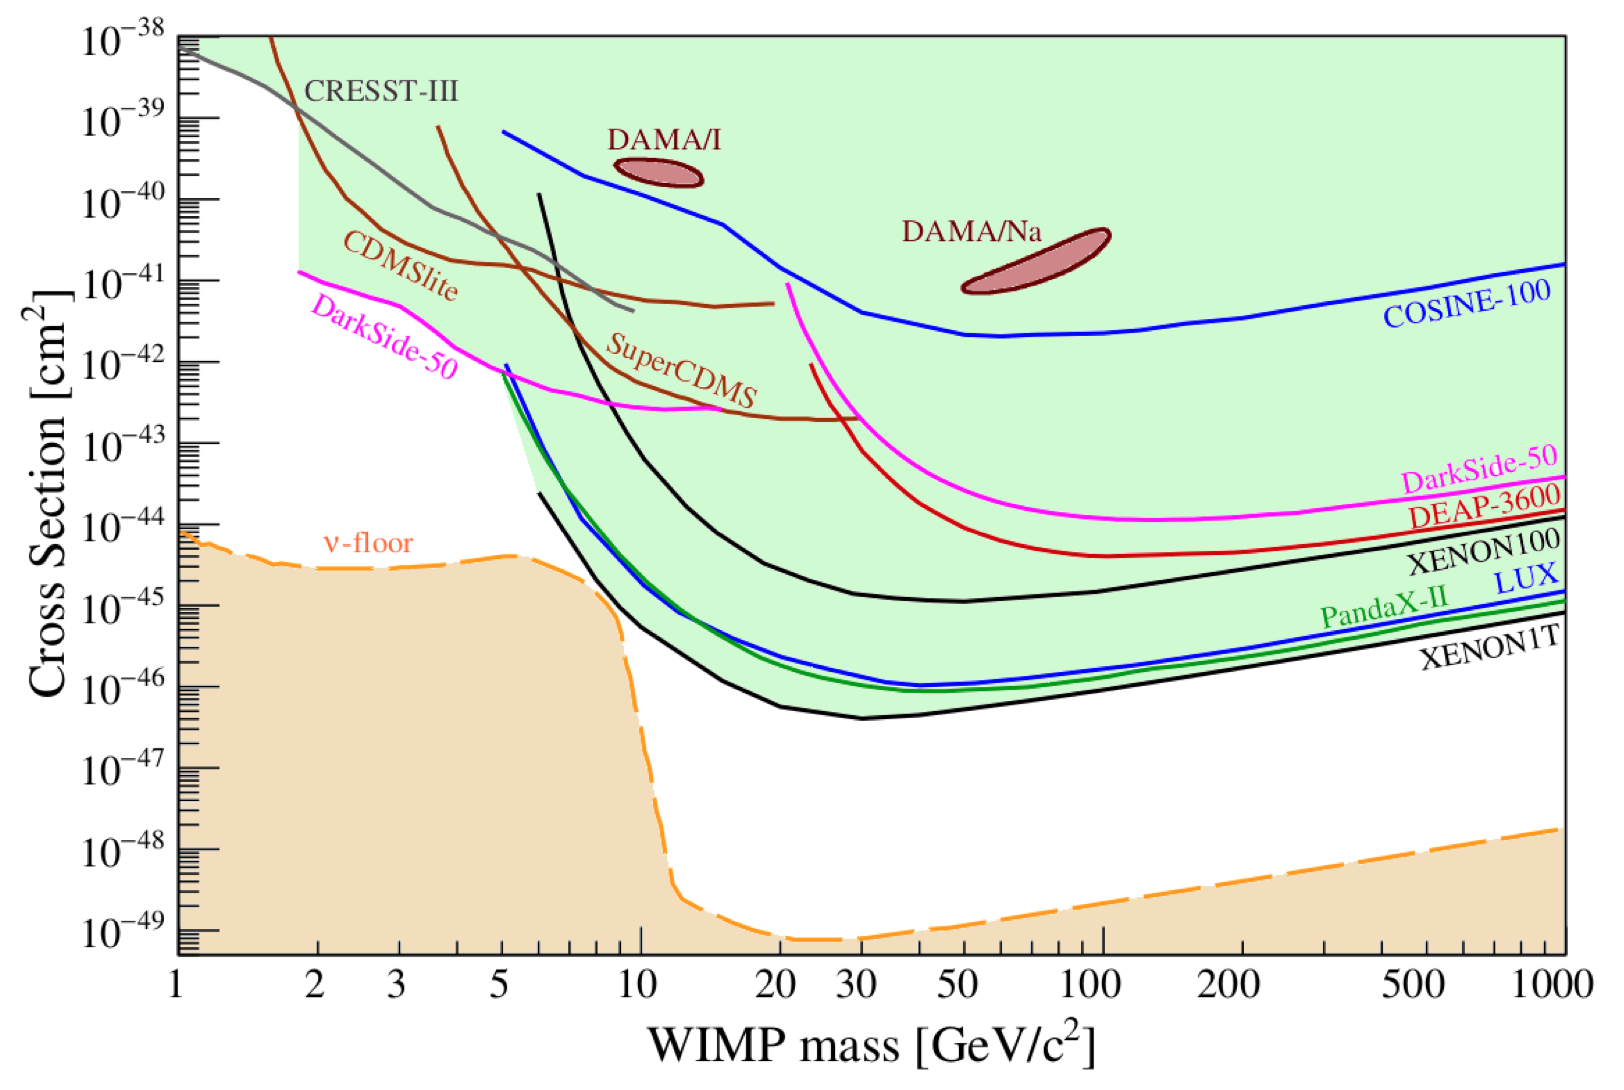
\includegraphics[width=0.95\textwidth]{figures/darkmatter/directdetection2019_si.png}
    \caption{Constraints placed on the SI WIMP-nucleon cross-section for WIMPs with mass \(m_{\chi}\) by direct detection experiments. Figure reproduced from Ref.~\cite{Schumann2019}.}
    \label{fig:dm:searches:dd:si}
\end{figure}

% \begin{figure}[htbp]
%     \centering
%     \begin{subfigure}{1.\textwidth}
%       \centering
%       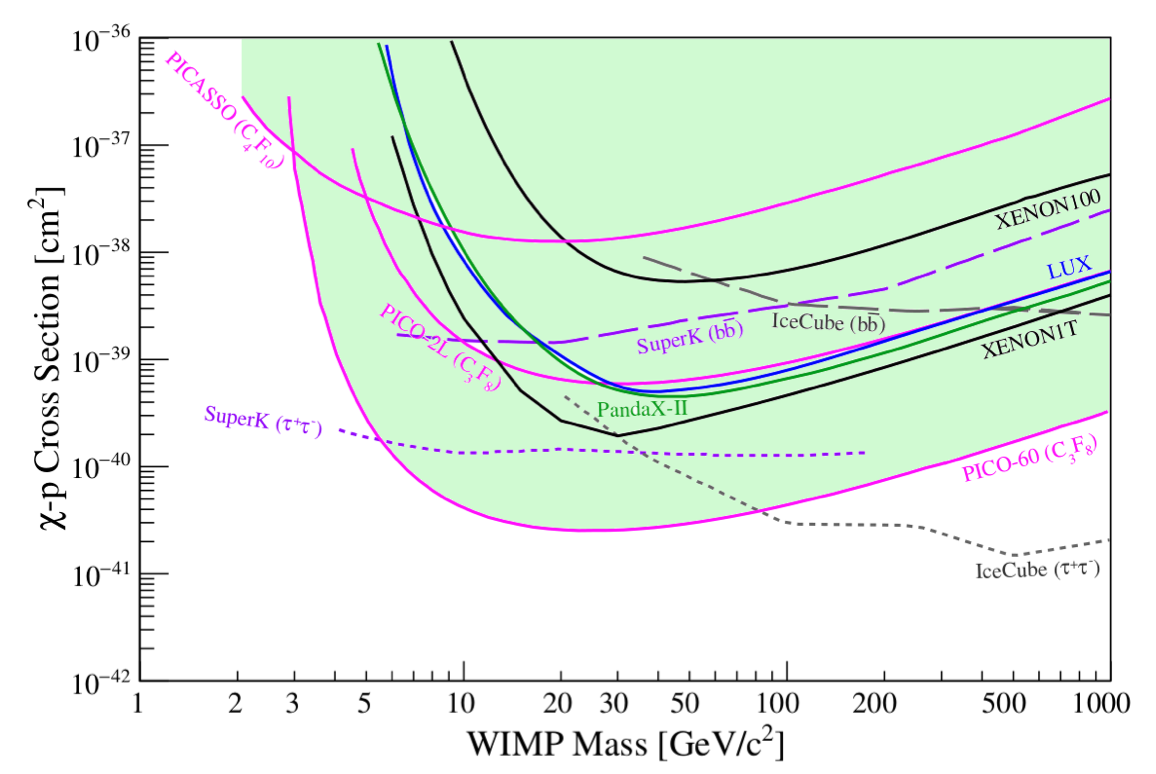
\includegraphics[width=.95\textwidth]{figures/darkmatter/directdetection2019_sdp.png}
%       \caption{WIMP-proton interactions}
%       \label{fig:dm:searches:dd:sd:wimp-proton}
%     \end{subfigure}
%     \\
%     \begin{subfigure}{1.\textwidth}
%       \centering
%       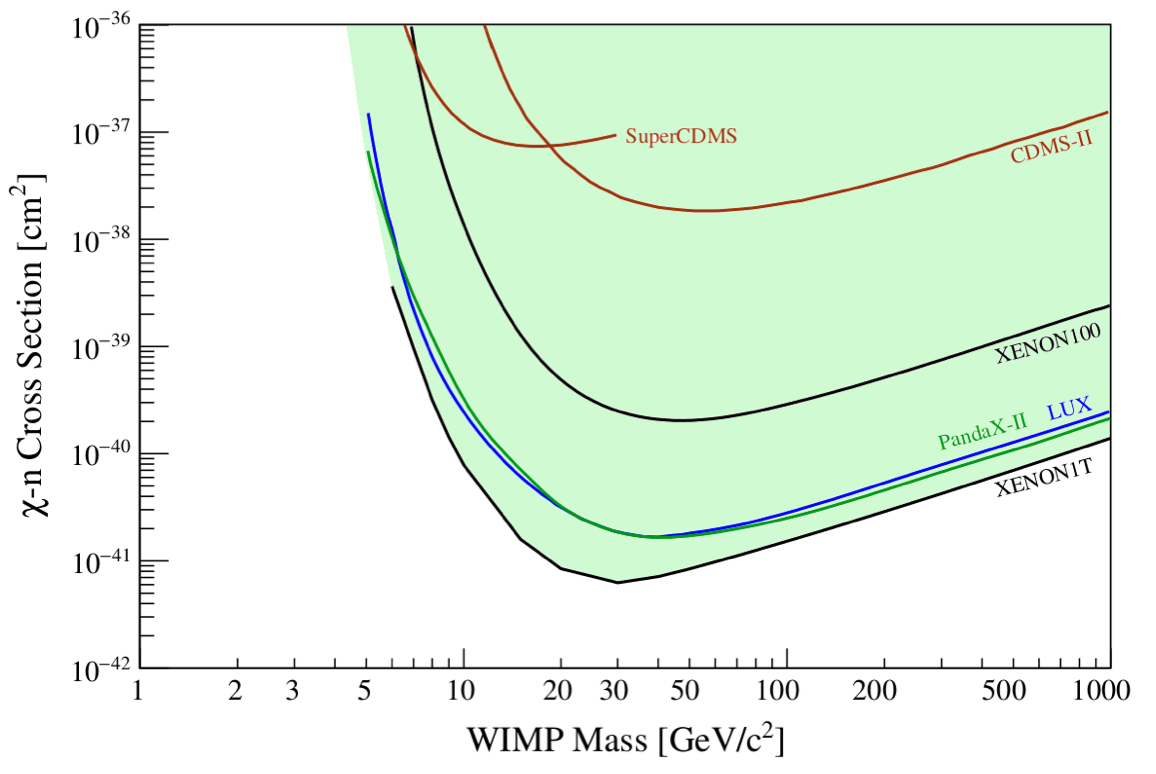
\includegraphics[width=.95\textwidth]{figures/darkmatter/directdetection2019_sdn.png}
%       \caption{WIMP-neutron interactions}
%       \label{fig:dm:candidates:constraints:axions}
%     \end{subfigure}
%     \caption{Constraints placed on the SD WIMP-nucleon cross-section for WIMPs with mass \(m_{\chi}\) by direct detection experiments. Figure reproduced from Ref.~\cite{Schumann2019}.}
%     \label{fig:dm:searches:dd:sd}
% \end{figure}

\subsection{Indirect detection experiments}
\label{sec:dm:searches:id}
Indirect detection experiments (c.f. Refs.~\cite{Conrad2017,losHeros2020} for a review) search for excess in flux of gamma rays, neutrinos or cosmic rays due to dark matter pair annihilation. WIMPs can annihilate in regions of large density, such as galaxy cores, the Sun or the Earth.

The gamma-ray, neutrino or cosmic ray flux (denoted \(x\)) from an object under consideration~\cite{losHeros2020}
\begin{align}
    \frac{\dd{\phi}}{\dd{E}_{x}} = \frac{1}{4 \pi} \frac{\langle \sigma_{\HepProcess{\chi \chi \to X}} v\rangle}{2 m_{\chi}^2} \frac{\dd{N_{x}}}{\dd{E_{x}}} \times \int \dd{\Omega} \int_{\text{line of sight}} \dd{r} \rho_{\chi}(r)^2
\end{align}
depends on
\begin{itemize}
    \item the thermally averaged product of the dark matter self-annihilation cross-section times the dark matter velocity \(\langle \sigma_{\HepProcess{\chi \chi \to X}} v\rangle\)
    \item the WIMP mass \(m_{\chi}\)
    \item the expected particle spectrum \(\dd{N_{x}}\dd{E_{x}}\), and
    \item the so-called ``J-factor'', the integrated squared dark matter density along the line of sight to the object under consideration \(\int_{\text{line of sight}} \rho_{\chi}(r)^2 \dd{r} \dd{\Omega}\).
\end{itemize}

Searches for gamma-ray emission have focused on nearby dwarf spheroidal galaxies with considerably low backgrounds, the inner region of the Milky Way with a considerable background at almost any wavelength, and nearby clusters of galaxies. A potential signal of dark matter annihilation manifests as a nearly mono-energetic line in the spectrum, with an energy close to the WIMP mass and a width proportional to the dark matter velocity~\cite{Tanabashi2018}.

A variety of different experiments aim for indirect detection of dark matter. The Fermi Large Area Telescope (LAT)~\cite{Atwood2009} and the ground-based facilities HESS~\cite{Aharonian2006}, VERITAS~\cite{Archambault2017}, HAWC~\cite{Abeysekara2018}, and MAGIC~\cite{Aleksi2016} probe the gamma-ray spectrum for WIMPs in the mass range \(\SI{1}{\giga\electronvolt} < m_{\chi} < \SI{10}{\tera\electronvolt}\). Fermi LAT observed an excess emission at energies of a few GeV in the gamma-ray flux from the galactic centre. Although several interpretations suggest compatibility with a potential signal~\cite{Hooper2011,Karwin2017}, this interpretation is subject of contestation~\cite{deBoer2017}.
Additional experiments looking for indirect detection are AMS~\cite{Aguilar2013}, PAMELA~\cite{Adriani2009}, and IceCube~\cite{Aartsen2013}.

\Cref{fig:dm:searches:id:overview} shows an overview of constraints on WIMPs from indirect detection experiments.
\begin{figure}[htbp]
    \centering
    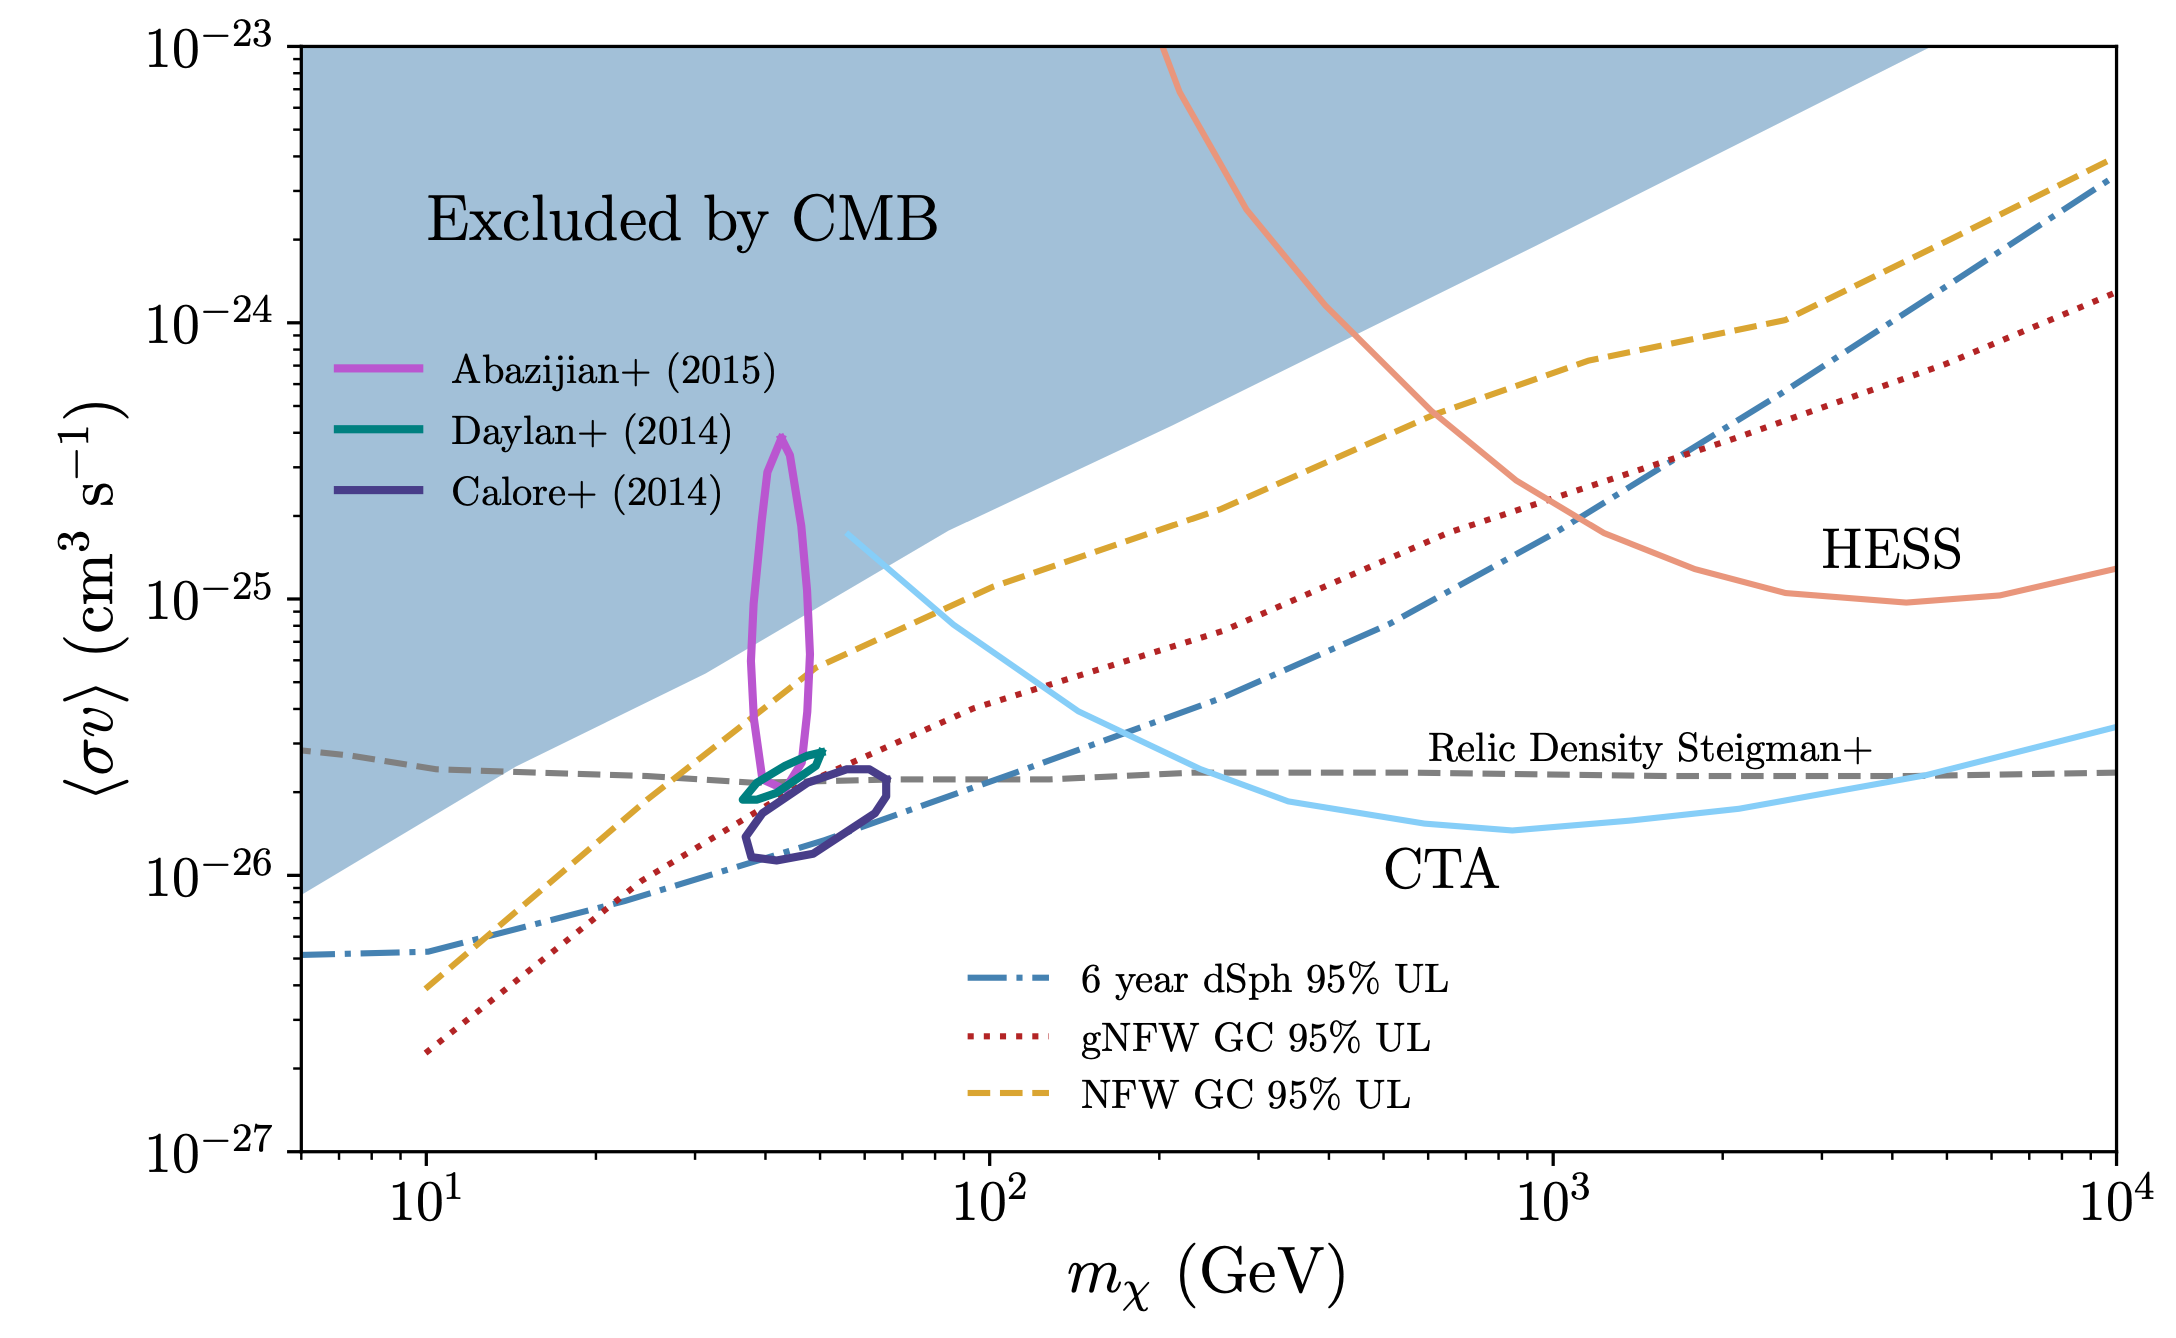
\includegraphics[width=0.95\textwidth]{figures/darkmatter/pdg_indirectdetection2020.png}
    \caption{Constraints placed on the self-annihilation cross-section for WIMPs with mass \(m_{\chi}\) by indirect detection experiments. Figure reproduced from Ref.~\cite{Tanabashi2018}.}
    \label{fig:dm:searches:id:overview}
\end{figure}

\subsection{Searches for dark matter at particle colliders}
\label{sec:dm:searches:collider}
Hadron collider searches (c.f. Ref.~\cite{Buchmueller2017} for a review) aim to detect signals of WIMPs produced when colliding proton beams in a controlled laboratory environment. Dark matter particles leave no trace in the detectors surrounding the collision point due to their feeble interactions with SM particles. The absence of a reconstructed particle trajectory allows inferring the presence of dark matter using momentum conservation in the plane perpendicular to the colliding beams. As the net transverse momentum before the collision is zero, it must also be so after the collision. An imbalance in the transverse plane is quantified by the missing transverse momentum \met, which is obtained as the negative vector sum of the transverse momenta of all detected particles. The characteristic signature for WIMP production at particle colliders is the observation of significant \met in association with one or more additional SM particles. This signature is known as ``\(\met + X\)'' and underpins the searches presented in this dissertation. The interaction between SM and dark matter particles typically takes place via a spin-1 or spin-0 mediator. The ATLAS and CMS experiments carry out a range of \(\met + X\) searches:
\begin{itemize}
    \item \met + jets,
    \item \met + photon \Pgg or weak vector boson \PWpm / \PZ,
    \item \met + heavy flavour quarks.
    \item \met + SM Higgs boson \Ph,
\end{itemize}
The \met + jets search~\cite{EXOT-2016-27,CMS-EXO-16-048} is one of the most inclusive types of searches by considering final states with one or more jets originating from initial state radiation. The accurate theoretical description of SM background processes, which is improved by data-driven methods, establishes the sensitivity to potential signals in the tails of the \met distribution.
Similarly, dark matter particles may be produced in association with a vector boson radiated off from a quark in the initial state.
The \met + photon searches~\cite{EXOT-2016-32,CMS-EXO-16-039} benefit from a very clean signature of \met and a high-energetic photon. The much lower backgrounds compared to the \met + jets search make up for the smaller production cross-section than for QCD radiation. The \met + weak vector boson searches can investigate different decay modes of the vector boson. While a leptonically decaying \PZ boson~\cite{HIGG-2016-28} also presents a very clean signature, the hadronic decay channel~\cite{CMS-EXO-16-037} is appealing due to the larger branching fraction.
The searches targeting \met + heavy flavour quarks~\cite{SUSY-2016-18,CMS-EXO-18-010,CMS-EXO-16-051,CMS-EXO-16-049} can probe dark matter production via the exchange of spin-0 mediators.
Finally, searches targeting the \met + SM Higgs boson final state can investigate the various decay modes of the Higgs boson~\cite{CMS-EXO-18-011}. The decay to \bquarks~\cite{EXOT-2016-25,ATLAS-CONF-2018-039} if favoured by having the largest branching fraction. Searches also explore the cleaner \HepProcess{\Ph \to \Pgtpm \Pgtmp}~\cite{CMS-EXO-16-055} and \HepProcess{\Ph \to \Pgg \Pgg}~\cite{HIGG-2016-18} final states with smaller branching fractions. Searches probing the invisible decay of the Higgs boson in vector-boson-fusion topology or associated production with vector bosons~\cite{HIGG-2016-28} serve as another test of the WIMP hypothesis.
To date, no collider search has made claims of discovery of dark matter.

A second approach in constraining dark matter models at colliders is searching for the visible decays of the mediators. Assuming the existence of such a mediator, at least the visible mediator decay to the same SM particles which produced the mediator -- quarks or gluons --- is guaranteed. Also, possible decays to leptons are considered. The signature of visible mediator decays is a narrow excess in the otherwise smoothly falling background spectrum of the invariant mass of two jets or leptons with the largest momentum. The ATLAS and CMS experiments carry out a range of dijet~\cite{EXOT-2019-03,CMS-EXO-16-032} or dilepton searches~\cite{CMS-EXO-16-056,}. While the high-mass dijet resonance searches constrain the mediator mass from \SI{1.5}{\tera\electronvolt} to \SI{3.5}{\tera\electronvolt}, the searches for low-mass dijet resonances are limited by the process high rates. Searches in this regime are enabled by recording only a limited amount of information of the full event record~\cite{EXOT-2016-20} or by requiring the presence of a resonance produced in association with an additional high-energetic particle or jet~\cite{EXOT-2018-05}.

The current status and perspectives for collider based dark matter searches are presented in \Cref{sec:outlook}.


\section{Theoretical frameworks for dark matter production at particle colliders}
\label{sec:dm:models}
The theoretical frameworks predicting the production of WIMPs are an indispensable part of collider searches. They guide the design and optimisation of the searches by elucidating the phenomenology of potential dark matter particle candidates in specific final states. In addition, they allow connecting the results of collider searches with direct and indirect detection experiments.

The range of models predicting dark matter production at the LHC varies in generality and plausibility. The two end-points of the spectrum are defined by the effective field theory (EFT) approach and complete theories, such as supersymmetry. \Cref{fig:dm:models:overview} shows an overview of theoretical frameworks describing dark matter production at particle colliders with varying degrees of completeness and complexity.
\begin{figure}[htbp]
    \centering
    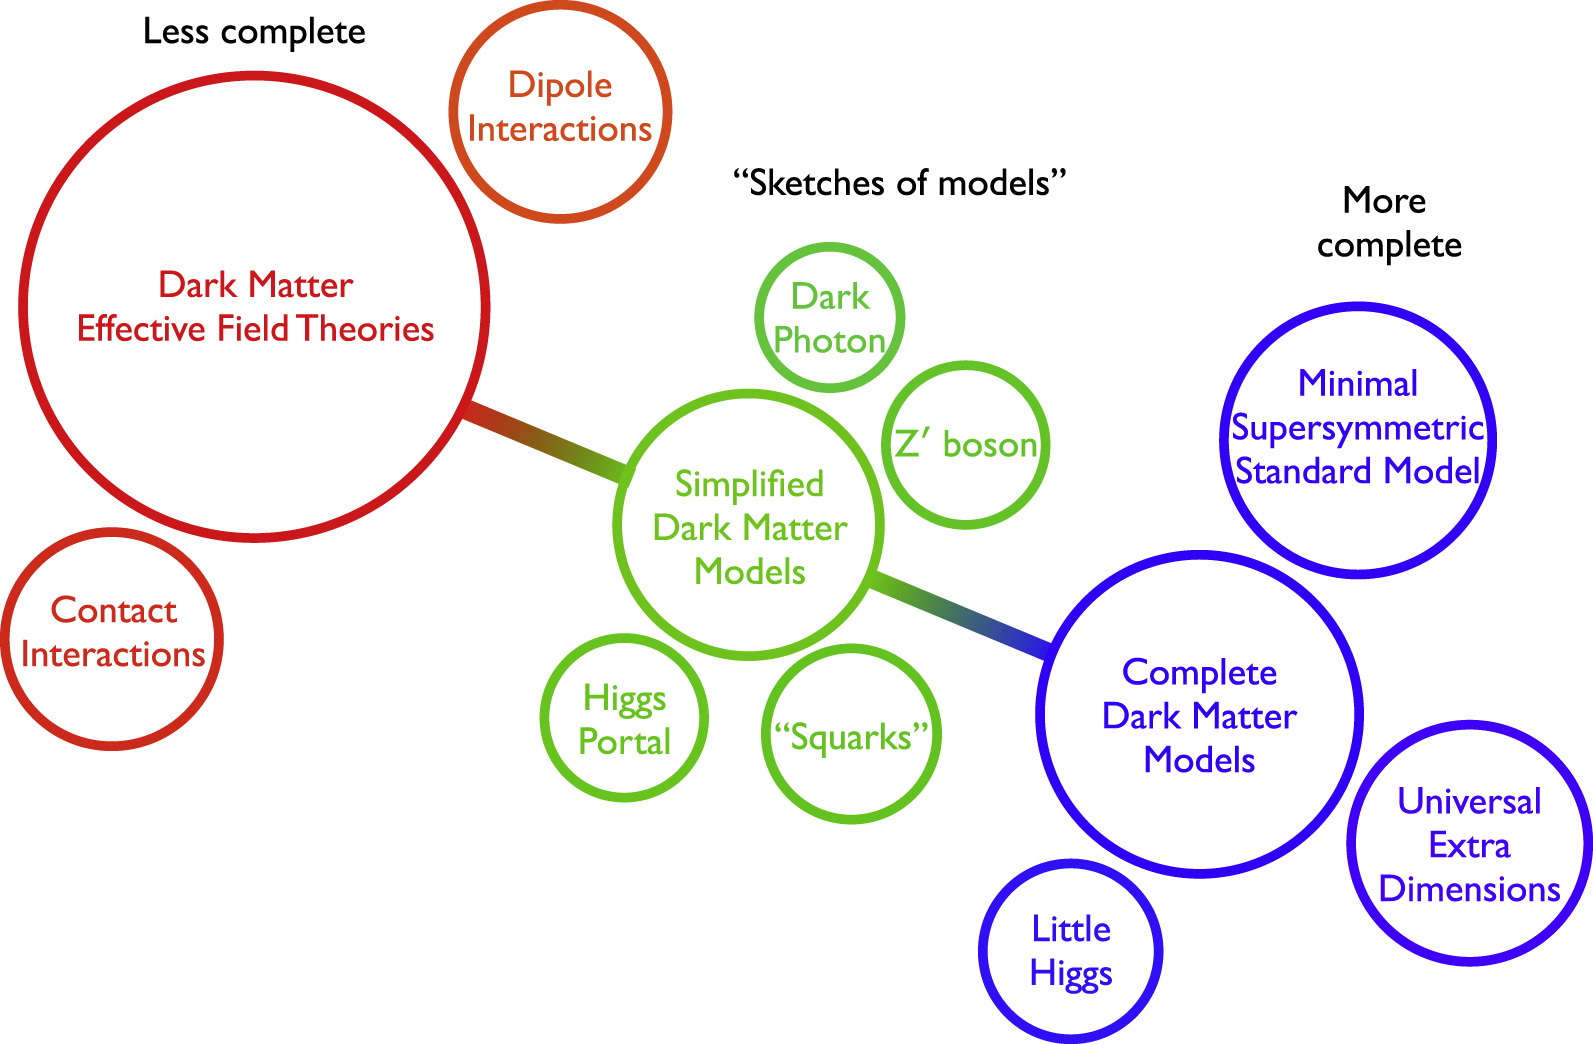
\includegraphics[width=0.95\textwidth]{figures/darkmatter/models.jpg}
    \caption{Overview of theoretical frameworks describing dark matter production at particle colliders. The models range from dark matter effective field theory, over various simplified models, to complete dark matter models. Figure reproduced from Ref.~\cite{Abdallah2015}.}
    \label{fig:dm:models:overview}
\end{figure}

The effective field theory (EFT) approach introduces the WIMP as the only additional state which is accessible at the LHC and describes its interaction with SM particles through a four-point effective contact interaction. Similar to Fermi's theory of weak interactions, heavy intermediate states are mapped to effective operators, which are characterised by the energy scale of the interaction.
Complete theoretical frameworks, on the other hand, are well-motivated and consistent theories with perturbative ultraviolet (UV) completions. They make specific predictions for invisible, heavy particles with mass at the electroweak scale. Typically, these complete theories are characterised by a large number of model parameters.

While the LHC experiments also have a broad array of searches in the context of complete theories, the dedicated LHC dark matter searches follow a theory-agnostic approach by specifying only the interaction between SM particles and WIMPs relevant to the signature of dark matter pair production.

It has been shown that the EFT approach is overly simplistic to capture the phenomenology of more complete models fully. Their kinematic distributions differ significantly from the ones obtained in an EFT description. Moreover, the EFT approach breaks down at the \si{\tera\electronvolt} energy scale probed in LHC interactions, as the momentum transfer in the process is sufficient to resolve the underlying processes.
As a consequence, the preferred theoretical framework of LHC dark matter searches are \emph{simplified models}, which make explicit assumptions about at least two additional states: a WIMP and a particle mediating the interaction between WIMP and SM particles. Scenarios with an SM mediator are almost ruled out, therefore suggesting the mediator to be a yet-undiscovered particle. Although simplified models are characterised by only a small number of parameters and make no assumptions about extended particle sectors, they can be designed to be fully consistent at all energy scales.

The searches for dark matter presented in this dissertation are motivated by a range of simplified models with varying degree of complexity. The following paragraphs discuss a simplified model for dark matter production with a spin-1 \PZprime mediator, two simplified models with an extended Higgs sector, and a simplified model with two mediators.

\subsection{Simplified model for dark matter production with a spin-1 \PZprime mediator}
\label{sec:dm:models:dmsimp}
The simplified model with a vector or axial-vector mediator (\(V/A\) simplified model)~\cite{Abercrombie2019} is a minimal extension of the SM describing the production of dark matter particles via \(s\)-channel exchange. The model postulates a Dirac fermion dark matter particle \(\chi\) with mass \mchi, which is charged under an additional \(\text{U}(1)\) gauge symmetry. Assuming that also some SM particles are charged under this group, dark matter pair production can occur via the exchange of a new \PZprime gauge boson of mass \mZp, which is referred to as the \emph{mediator}. Both vector and axial-vector couplings between the spin-1 mediator are possible. The corresponding interaction Lagrangian densities are (neglecting mediator couplings to leptons with coupling strength \gl)
\begin{align}
    \mathcal{L}_{\text{vector}} &= \gq \sum_{q=\Pup, \Pdown, \Pstrange, \Pcharm, \Pbottom, \Ptop} \PZprime_{\mu} \overline{q} \gamma^{\mu} q + \gchi \PZprime_{\mu} \overline{\chi} \gamma^{\mu} \chi \\
    \mathcal{L}_{\text{axial-vector}} &= \gq \sum_{q=\Pup, \Pdown, \Pstrange, \Pcharm, \Pbottom, \Ptop} \PZprime_{\mu} \overline{q} \gamma^{\mu} \gamma^{5} q + \gchi \PZprime_{\mu} \overline{\chi} \gamma^{\mu} \gamma^{5} \chi
    \label{eq:dm:model:dmsimp}
\end{align}

The mediator couples universally to all quarks and leptons with the coupling strengths \gq and \gl, respectively, and couples to dark matter particles \(\chi\) with coupling strength \gchi~\cite{Albert2019}. The universal coupling to all quarks or leptons ensures that the general structure of flavour-changing neutral current processes is preserved in the extension of the SM via Minimal Flavour Violation~\cite{DAmbrosio2002}. Assuming that no additional visible or invisible decays contribute to the width of the mediator and ignoring possible decays to leptons, the minimal width is fixed by the couplings \gq and \gchi. The minimal widths for the vector and axial vector mediator are
\begin{align}
    \Gamma^{V}_{\text{min}} = & \Gamma^{V}_{\HepProcess{\chi \chi}} + \Gamma^{V}_{\HepProcess{\Pq\Pq}}\\
   = & \frac{\gchi^2 \mZp}{12 \pi} \left(1 + \frac{2 \mchi^2}{\mZp^2}\right) \beta_{\chi} \theta(\mZp - 2 \mchi) \nonumber \\
    & + \sum_{q=\Pup, \Pdown, \Pstrange, \Pcharm, \Pbottom, \Ptop} \frac{3 \gq^2 \mZp}{12 \pi} \left(1 + \frac{2 m_{\Pq}^2}{\mZp^2}\right) \beta_{\Pq} \theta(\mZp - 2 m_{\Pq}) \nonumber \\
	\Gamma^{A}_{\text{min}} = & \Gamma^{A}_{\HepProcess{\chi \chi}} + \Gamma^{A}_{\HepProcess{\Pq\Pq}}\\
   = & \frac{\gchi^2 \mZp }{12 \pi} \beta^3_{\chi} \theta(\mZp - 2 \mchi) \nonumber \\
	& + \sum_{q=\Pup, \Pdown, \Pstrange, \Pcharm, \Pbottom, \Ptop} \frac{3 \gq^2 \mZp}{12 \pi} \beta^3_{\Pq} \theta(\mZp - 2 \mchi), \nonumber
\end{align}
where \(\theta\) denotes the Heaviside step function and \(\beta_f = \sqrt{1 - 4 m_{f}^2 / \mZp^2}\) is the velocity of the fermion \(f\) with mass \(m_{f}\) in the rest frame of the \PZprime mediator.

Under the minimal width assumption, the model is specified by the set of parameters shown in \Cref{tab:dm:models:dmsimp:parameters}.
\begin{table}[hbt]
\caption{Parameters in the \(V/A\) simplified model}
\label{tab:dm:models:dmsimp:parameters}
\centering
\begin{tabular}{ll}
\toprule
Parameter & Description \\
\midrule
\mZp & \PZprime mediator mass \\
\mchi & dark matter particle mass \\
\gq & coupling strength of \PZprime mediator to quarks \\
\gl & coupling strength of \PZprime mediator to leptons \\
\gchi & coupling strength of \PZprime mediator to dark matter particles \\
\bottomrule
\end{tabular}
\end{table}

Both the vector mediator and the axial-vector mediator model are available in event generators up to next-to-leading order (\NLO) accuracy in QCD.

\subsection{Simplified model with an extended Higgs sector and a pseudo-scalar mediator}
\label{sec:dm:models:ahdm}
The \ahdm~\cite{Bauer2017} is a self-consistent simplified model with an extended Higgs sector, allowing the model to be embedded in a UV-complete and renormalisable framework. It is based on a Two-Higgs-doublet model (2HDM)~\cite{Branco2012} with five physical scalar states in the Higgs sector and an additional pseudo-scalar mediator.

The 2HDM potential for the two Higgs doublets \(H_{1}, H_{2}\) is given by
\begin{align}
    V_{H} = &\mu_{1} H_{1}^{\dagger} H_{1} + \mu_{2} H_{2}^{\dagger} H_{2} + (\mu_{3} H_{1}^{\dagger} H_{2} + \text{h.c.}) \nonumber \\
    & + \lambda_{1} (H_{1}^{\dagger} H_{1})^2 + \lambda_{2} (H_{2}^{\dagger} H_{2})^2 + \lambda_{3} (H_{1}^{\dagger} H_{1}) (H_{2}^{\dagger} H_{2}) \nonumber \\
    & + \lambda_{4} (H_{1}^{\dagger} H_{2}) (H_{2}^{\dagger} H_{1}) + \left[\lambda_{5} (H_{1}^{\dagger} H_{2})^2 + \text{h.c.}\right],
\end{align}
where \(\text{h.c.}\) denotes the Hermitian conjugate and \(\mu_{i}, i=1,2,3\) and \(\lambda_{i}, i=1,\dots,5\) are free parameters. The potential is CP-conserving and has a softly broken \(\mathbb{Z}_{2}\) custodial symmetry to suppress flavour-changing neutral currents. The Higgs doublets have the vacuum expectation values \(\langle H_{i} \rangle = (0, v_{i} / \sqrt{2})^{T}, i=1,2\) with \(v = \sqrt{v_{1}^2 + v_{2}^2} = \SI{246}{\giga\electronvolt}\) and their ratio defines \(\tan \beta = v_2 / v_1\). The physical CP-even states \Ph and \PH result from mixing of the  neutral CP-even weak eigenstates with a corresponding mixing angle \(\alpha\). The extended Higgs sector contains also two charged states \PHpm of identical mass.

The interaction term for the pseudo-scalar mediator \(P\)
\begin{align}
    V_{P} = \frac{1}{2} m_{P}^2 P^2 + P(i b_{P} H_{1}^{\dagger} H_{2} + \text{h.c.}) + P^2 (\lambda_{P_{1}} H_{1}^{\dagger} H_{1} + \lambda_{P_{2}} H_{2}^{\dagger} H_{2}),
\end{align}
with the pseudo-scalar mass parameter \(m_{P}\) and the portal couplings \(b_{P}, \lambda_{P_{1}}, \lambda_{P_{2}}\),
mixes the mediator with the CP-odd state in the extended Higgs sector with mixing angle \(\theta\). The resulting physical CP-odd states are \(a\) and \PA.

The dark matter particle \(\chi\) is a Dirac fermion with mass \(m_{\chi}\). The pseudo-scalar mediator couples to the dark matter particle with the real Yukawa coupling \(y_{\chi}\) via
\begin{align}
    \mathcal{L}_{\chi} = - i y_{\chi} P \overline{\chi} \gamma_{5} \chi.
\end{align}

The alignment limit \(\sin{(\beta - \alpha)} = 1\) is assumed, allowing the identification of the lightest CP-even scalar \Ph with the SM Higgs boson. A type-II 2HDM coupling structure is assumed, letting up- and down-type quarks couple to separate doublets. The model is specified by the set of 14 parameters shown in \Cref{tab:dm:models:ahdm:parameters}.
\begin{table}[hbt]
\caption{Parameters in the \ahdm simplified model}
\label{tab:dm:models:ahdm:parameters}
\centering
\begin{tabular}{ll}
\toprule
Parameter & Description \\
\midrule
\(\alpha\) & mixing angle of neutral CP-even weak eigenstates \\
\(\tan{\beta}\) & ratio of Higgs doublet vacuum expectation values \\
\(\theta\) & mixing angle of neutral CP-odd weak eigenstates \\
\(v\) & electroweak vacuum expectation value \\
\(\lambda_{3}, \lambda_{P_{1}}, \lambda_{P_{2}}\) & quartic couplings of scalar bosons \\
\(m_{\Ph}, m_{\PH}\) & masses of neutral CP-even Higgs bosons \\
\(m_{a}, m_{\PA}\) & masses of neutral CP-odd Higgs bosons \\
\(m_{\PHpm}\) & charged Higgs bosons mass \\
\(m_{\chi}\) & dark matter particle mass \\
\(y_{\chi}\) & Yukawa coupling of dark matter particle \\
\bottomrule
\end{tabular}
\end{table}

The \ahdm model is characterised by a rich phenomenology so that it can be probed by all \met + X searches, which are discussed in \Cref{sec:dm:searches:collider}. In particular, the \met + Higgs boson and \met + \PZ boson final states are expected to provide leading constraints in the theoretically best-motivated region of the parameter space.

\subsection{\zhdm simplified model}
\label{sec:dm:models:zp2hdm}
The \zhdm~\cite{Berlin2014} is another simplified model with an extended Higgs sector. It is based on a 2HDM (c.f. the discussion in \Cref{sec:dm:models:ahdm}) with an additional \(\text{U}(1)_{\PZprime}\) symmetry, which gives rise to a \PZprime boson. The \PZprime boson can mix with the \PZ boson. It is implicitly assumed that there is a mechanism for generating the \PZprime boson mass in a gauge-invariant way.

After symmetry breaking, the two Higgs doublets can be parametrised as
\begin{align}
H_{1} &= \begin{pmatrix} -\PHpm \sin \beta \\ v_{1} - \Ph \sin \alpha + \PH \cos \alpha - i \PA \sin \beta \end{pmatrix}\\
H_{2} &= \begin{pmatrix} \PHpm \cos \beta \\ v_{2} + \Ph \cos \alpha + \PH \sin \alpha + i \PA \cos \beta \end{pmatrix},
\end{align}
where similar conventions for denoting the Higgs doublets, the states in the extended Higgs sector and the mixing angles have been adopted as in \Cref{sec:dm:models:ahdm}.
The alignment limit \(\sin{(\beta - \alpha)} = 1\) is assumed, allowing the identification of the lightest CP-even scalar \Ph with the SM Higgs boson. The model specifies a type-II 2HDM coupling structure, letting up- and down-type quarks couple to separate doublets.
As only the right-handed up-type quarks \(\Pqu_{i, R}\) and the Higgs doublet \(H_{1}\) are charged under \(\text{U}(1)_{\PZprime}\), the \PZprime boson only couples to the Higgs doublet which couples to the up-type quarks and to right-handed quarks.
The CP-odd physical state \PA in the extended Higgs sector couples to dark matter particles.

The model is specified by the set of nine parameters shown in \Cref{tab:dm:models:zhdm:parameters}.
\begin{table}[hbt]
\caption{Parameters in the \zhdm simplified model}
\label{tab:dm:models:zhdm:parameters}
\centering
\begin{tabular}{ll}
\toprule
Parameter & Description \\
\midrule
\(\alpha\) & mixing angle of neutral CP-even weak eigenstates \\
\(\tan{\beta}\) & ratio of Higgs doublet vacuum expectation values \\
\(m_{\Ph}, m_{\PH}\) & masses of neutral CP-even Higgs bosons \\
\(m_{\PHpm}\) & mass of charged Higgs bosons \\
\mA & neutral CP-odd Higgs boson mass \\
\mZp & \PZprime boson mass \\
\(g_{\PZprime}\) & coupling strength of the \PZprime boson \\
\mchi & dark matter particle mass\\
\bottomrule
\end{tabular}
\end{table}

The model describes resonant production of a \PZprime boson, which subsequently decays into the SM Higgs boson \Ph and the CP-odd Higgs boson \PA. The latter enables dark matter pair production due to its large branching fraction to dark matter.

\subsection{Two mediator dark matter model}
\label{sec:dm:models:2mdm}
The two mediator dark matter model~\cite{Duerr2016,Duerr2017} (2MDM model) is a consistent simplified model with a \PZprime boson and a dark Higgs boson as mediators. The model postulates a Majorana fermion as dark matter particle \(\chi\), a complex Higgs field \(S\) and an additional \(\text{U}(1)_{\PZprime}\) gauge group. It satisfies the requirements of gauge invariance and perturbative unitarity by incorporating more features of complete theories: the masses of the fermionic dark matter particle and of the \PZprime boson are generated by spontaneous symmetry breaking of the \(\text{U}(1)_{\PZprime}\) group. The symmetry breaking gives rise to the dark Higgs boson \(s\). The dark matter particle \(\chi\) with mass \(m_{\chi}\) couples via axial coupling to the \PZprime boson. The interaction Lagrangian density is
\begin{align}
    \mathcal{L}_{\chi} = - \frac{1}{2} g_{\chi} \PZprime^{\mu} \overline{\chi} \gamma^{5} \gamma_{\mu} \chi - g_{\chi} \frac{m_{\chi}}{m_{\PZprime}} s \overline{\chi} \chi + 2 g_{\chi} \PZprime^{\mu} \PZprime_{\mu} (g_{\chi} s^2 + m_{\PZprime} s).
\end{align}
with the four independent parameters
\begin{itemize}
	\item dark matter particle mass \mchi,
	\item \PZprime boson mass \mZp,
	\item dark Higgs boson mass \ms,
	\item \(\gchi = g_{\PZprime} q_{\chi}\) dark matter coupling, with the \(\text{U}(1)_{\PZprime}\) gauge coupling \(g_{\PZprime}\) and charge of the dark matter particle \(q_{\chi} = q_{S} / 2\).
\end{itemize}

The dark sector is coupled to the SM by postulating vector couplings of the \PZprime to quarks (\Pq) by gauging baryon number. The corresponding interaction Lagrangian is
\begin{align}
    \mathcal{L}_{q} = - \gq \PZprime^{\mu} \Paq \gamma_{\mu} \Pq
\end{align}
with the coupling strength of the \PZprime boson to quarks \gq. Axial-vector couplings and couplings to leptons are neglected for simplicity.


The model is specified by the set of five parameters shown in \Cref{tab:dm:models:2mdm:parameters}.
\begin{table}[hbt]
\caption{Parameters in the two mediator dark matter simplified model}
\label{tab:dm:models:2mdm:parameters}
\centering
\begin{tabular}{ll}
\toprule
Parameter & Description \\
\midrule
\mchi & dark matter particle mass \\
\mZp & \PZprime mediator mass \\
\ms & the dark Higgs boson mass \\
\gchi & coupling strength of \PZprime mediator to dark sector \\
\gq & coupling strength of \PZprime mediator to quarks \\
\(\theta\) & mixing angle between the SM Higgs boson \\
           & and the dark Higgs boson \\
\bottomrule
\end{tabular}
\end{table}

The model can be thought of as a combination of two simplified models: one with a spin-1 mediator (c.f. \Cref{sec:dm:models:dmsimp}) and one with a spin-0 mediator. In this dissertation, the resonant production of a dark Higgs boson decaying to SM particles is investigated.

Non-zero mixing between the dark Higgs boson and the SM Higgs boson with mixing angle \(\theta\) ensures that the dark Higgs boson is unstable and can instantly decay into SM states. Consequentially, the dark Higgs boson inherits the branching fractions of an SM-like Higgs boson with mass \ms, which are shown in \Cref{fig:dm:models:2mdm:darkhiggsbranching}.

\begin{figure}[htbp]
    \centering
    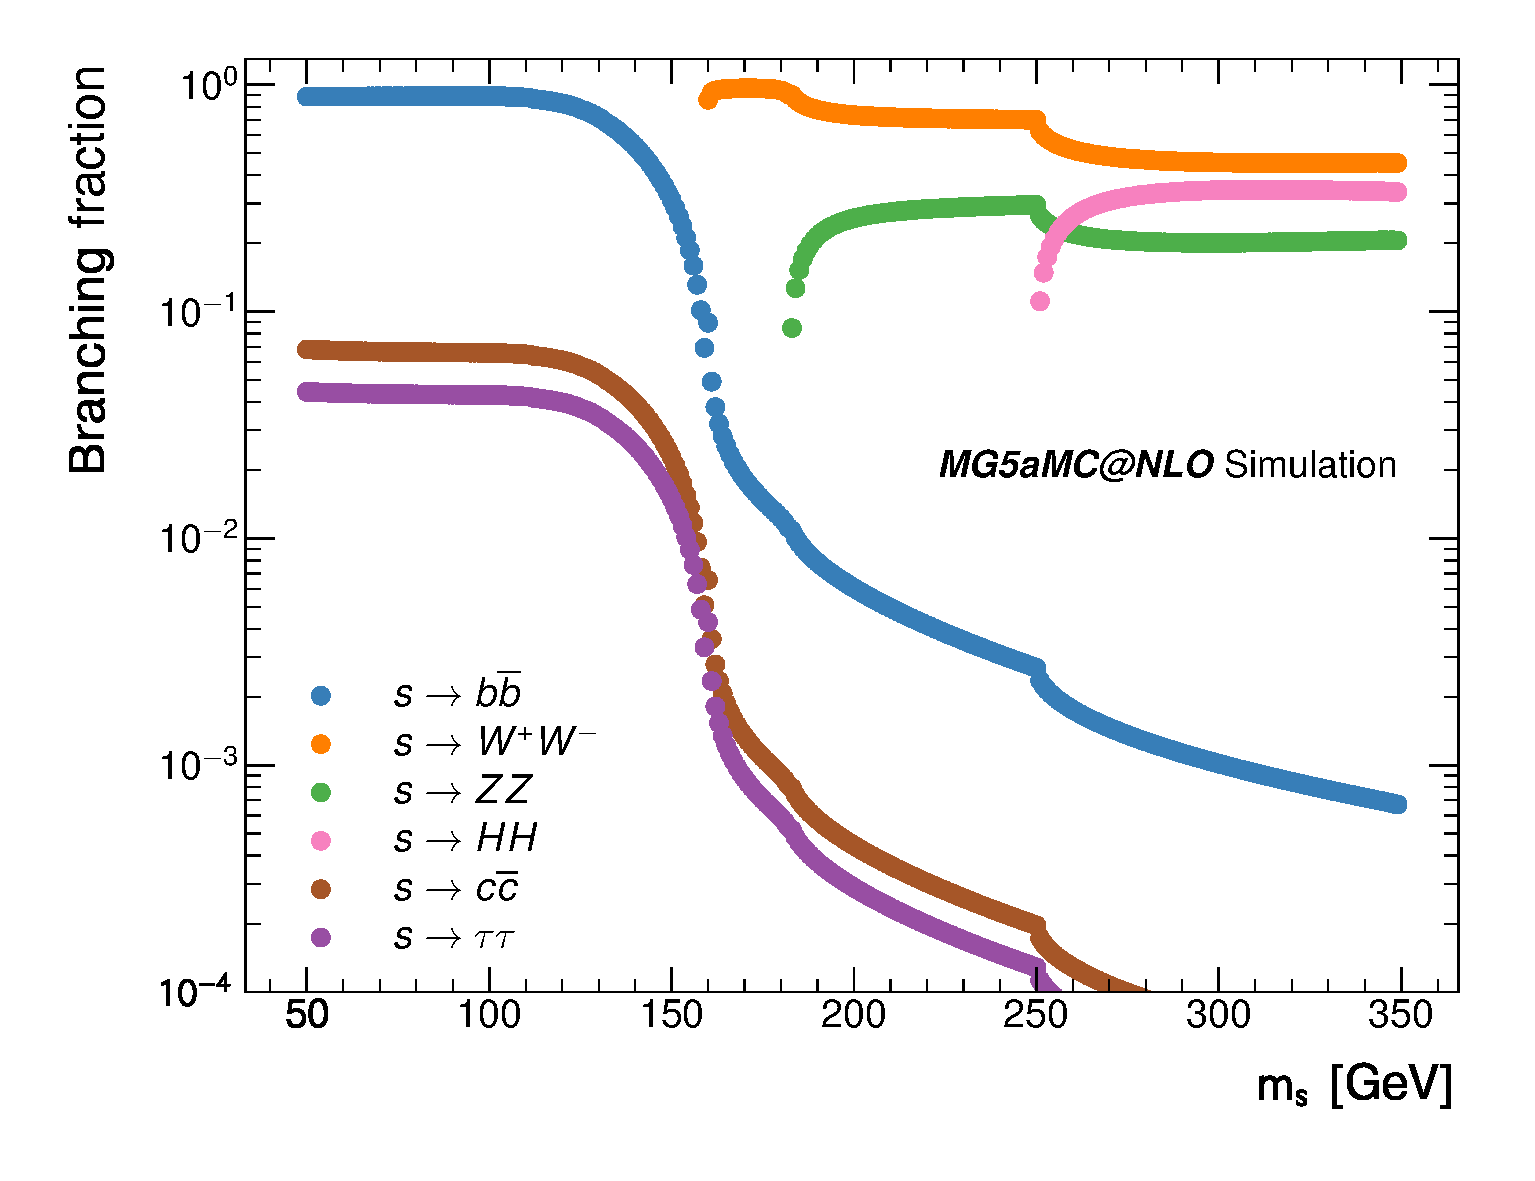
\includegraphics[width=0.95\textwidth]{figures/darkmatter/darkhiggs_branchingfraction.pdf}
    \caption{Branching fractions of dark Higgs boson decays to SM particles (produced on-shell) in dependence of \ms.}
    \label{fig:dm:models:2mdm:darkhiggsbranching}
\end{figure}

% % !TEX root = ../my-thesis.tex
%
\chapter{Proton-proton collision phenomenology}
\label{sec:pp}

\section{Basic concepts}
\label{sec:pp:basics}
Collisions of protons at high energy scales can be described by perturbative quantum field theory. Matrix elements of strong interaction processes can be calculated systematically at fixed orders in the strong coupling constant \(\alpha_{s}\). However, the description of \HepProcess{\Pp\Pp} collision events involves additional complexity, as protons are strongly interacting and composite objects. In \HepProcess{\Pem\Pep} collisions, the participants in the scattering process are the same elementary particles which are accelerated. In contrast, in a typical \HepProcess{\Pp\Pp} collision, it is the proton beams which are accelerated but two partons which take part in the hard scattering process. The debris of the initial protons gives rise to additional activity in the event.
Furthermore, the interactions which convert the coloured parton states into hadrons occur at low momentum scale, where the strong coupling becomes large, and consequently, they cannot be described by perturbation theory.

The detailed description of a \HepProcess{\Pp\Pp} collision event can be decomposed into various processes. \Cref{fig:pp:collision} shows a proton-proton collision event with the production of a top quark pair and a Higgs boson in the hard scattering process. The various colours encode different processes, which are listed ordered by the respective momentum transfer \(Q^2\), starting with the hardest process.
\begin{figure}[htbp]
	\centering
	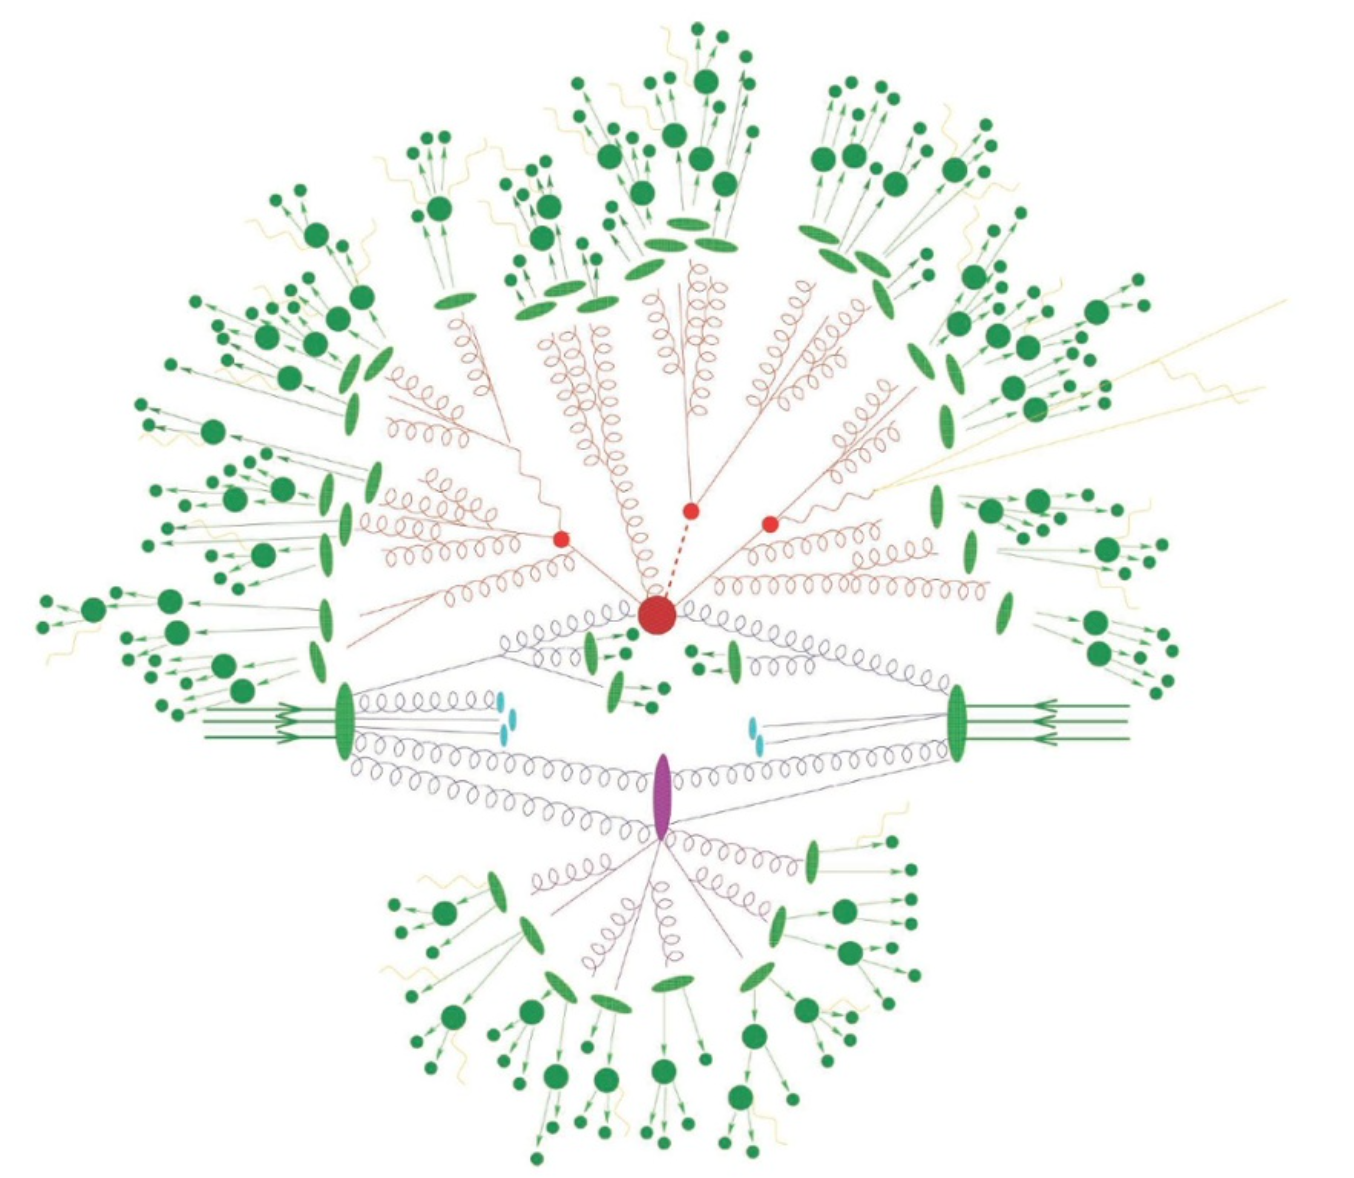
\includegraphics[width=0.95\textwidth]{figures/protoncollisions/pp-event.png}
	\caption{Sketch of a proton-proton collision event in which a top quark pair and a Higgs boson are produced in the hard scattering process. The incoming protons are shown as the central green ellipses with three incoming valence quark lines. The hard scattering process is depicted as the central red blob. The initial and final state radiation processes are shown in blue and red, respectively. The underlying event of other partons scattering and producing further activity is shown in purple. All emerging partons undergo hadronisation, resulting in cascading showers of hadrons, which are shown in green. Figure reproduced from Ref.~\cite{Campbell2018}.}
	\label{fig:pp:collision}
\end{figure}
\begin{enumerate}
	\item Hard interaction (red)
	\item Initial state radiation (ISR) (blue)
	\item Final state radiation (FSR) (red)
	\item Hadronisation and hadron decays (green)
	\item Underlying event (purple)
\end{enumerate}

The hard scattering process involves the largest momentum scales, allowing for a description at fixed-order perturbation theory in QCD. The description of the hard scattering process includes the relevant features of the event, such as the production of heavy states or hard QCD jets. Typically, the description of the hard scattering process is achieved by automated evaluation of the relevant Feynman diagrams and numerical integration over the phase-space of the final state particles.
Secondary emissions include ISR from the incident partons and FSR from the particles produced in the hard scattering process. The ISR originates from the breakdown of the coherent quantum states initiated by the parton taking part in the hard interaction. The FSR is due to Bremsstrahlung of particles produced in the hard scattering process, which results in the emission of particles at lower scales. The emitted QCD radiation initiates a parton shower via parton fragmentation, c.f. the splitting processes \HepProcess{\Pq \to \Pq \Pgluon}, \HepProcess{\Pgluon \to \Pgluon \Pgluon}, and \HepProcess{\Pgluon \to \Pq \Paq}. As the result of the parton shower, a set of coloured partons at the scale of a few \si{\giga\electronvolt} emerges. At this momentum scale, confinement becomes relevant, and the coloured parton states break up into a primary generation of colour-neutral hadrons. This process is called hadronisation. The description of this process involves simulation in non-perturbative models. The most prominent models are the Lund string model~\cite{Andersson1983} and the cluster model~\cite{Webber1984,Marchesini1988,Marchesini1992}. These initial hadrons decay further in cascades of hadrons, resulting in the formation of QCD jets.
The underlying event refers to multi-parton interactions in the event, which are difficult to model. Typically, the momentum transfer in these additional parton interactions is soft compared to the hard interaction. The description of the underlying event employs models with tunable parameters.

\section{Parton density functions}
\label{sec:pp:pdfs}
A key insight of the parton model is that the quarks and gluons inside a proton can be described in terms of parton density functions (PDFs) \(f_{a / \Pp}(x, Q^2)\) that parametrise the probability of finding a parton \(a\) with momentum fraction \(x\) at a scale of \(Q^2\) inside a proton.
PDFs can be measured in different processes and at different scales. These can be related to each other by the Dokshitser-Gribov-Lipatov-Altarelli-Parisi (DGLAP) equations~\cite{Dokshitzer1977,Gribov1972,Altarelli1977}
\begin{align}
    \frac{\partial}{\partial \log Q^2} \begin{pmatrix} f_{q/\Pp}(x, Q^2) \\ f_{g/\Pp}(x, Q^2) \end{pmatrix} = \frac{\alpha_{s}(Q^2)}{2\pi} \int_{x}^{1} \frac{\dd{z}}{z} \begin{pmatrix} \mathcal{P}_{qq}(\frac{x}{z}) \mathcal{P}_{qg}(\frac{x}{z}) \\ \mathcal{P}_{gq}(\frac{x}{z}) \mathcal{P}_{gg}(\frac{x}{z}) \end{pmatrix} \begin{pmatrix} f_{q / \Pp} (z, Q^2) \\ f_{g / \Pp} (z, Q^2) \end{pmatrix}.
\end{align}
The splitting functions \(\mathcal{P}_{gg}(\frac{x}{z})\) can be expanded in perturbation theory and are listed, for instance, in Ref.~\cite{Campbell2018}.

The PDFs can be determined from fits to a wide range of experimental data. In typical PDF fits, about \num{3000} data points are used ~\cite{Campbell2018}, including deep inelastic scattering data from fixed-target experiments and the HERA electron-proton collider, and data from Drell-Yan and jet production processes at the Tevatron and the Large Hadron Collider. The CT14~\cite{Dulat2016}, MMHT2014~\cite{HarlandLang2015}, and NNPDF3.0~\cite{Ball2015} PDF sets are the primary choices to describe proton-proton collisions at the Large Hadron Collider~\cite{Butterworth2016} and provide PDFs at leading order (\LO), next-to-leading order (\NLO) and next-to-next-to-leading order (\NNLO) precision in \(\alpha_{s}\).

\Cref{fig:pp:pdfs:ct14} shows the PDFs from the CT14 PDF set for the scales \(Q^2 = \SI{2}{\square\giga\electronvolt}\) and \(Q^2 = \SI{100}{\square\giga\electronvolt}\). The proton valence quark PDFs (\Pqu and \Pqd) are the largest for high \(x\)-values, while the sea-quark and gluon PDFs dominate at low \(x\)-values. For higher scale \(Q^2\), the gluon and sea-quark contributions are enhanced together with the valence quarks at low \(x\)-values, as more parton structure is resolved.
\Cref{fig:pp:pdfs:comparison} shows a comparison of the CT14 PDF set to the MMHT2014 and NNPDF3.0 PDF sets with their respective uncertainty bands. The discrepancies between different PDF sets originate from different input data, different choices for the parameters and PDF parametrisation.

\begin{figure}[htbp]
	\centering
    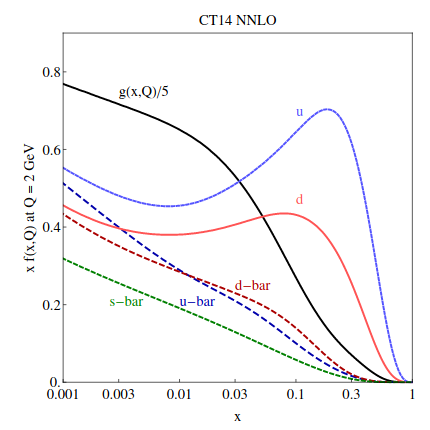
\includegraphics[width=.75\textwidth]{figures/protoncollisions/pdf_ct14_q2.png} \\
    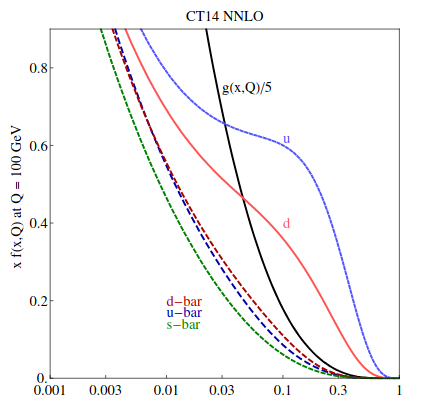
\includegraphics[width=.75\textwidth]{figures/protoncollisions/pdf_ct14_q100.png}
    \caption{The CT14 parton distribution functions at the scales of \SI{2}{\giga\electronvolt} (top) and \SI{100}{\giga\electronvolt} (bottom) for \Pqu \Paqu, \Pqd, \Paqd, \Paqs, and \Pgluon. Figure reproduced from Ref.~\cite{Dulat2016}.}
    \label{fig:pp:pdfs:ct14}
\end{figure}

\begin{figure}[htbp]
    \centering
    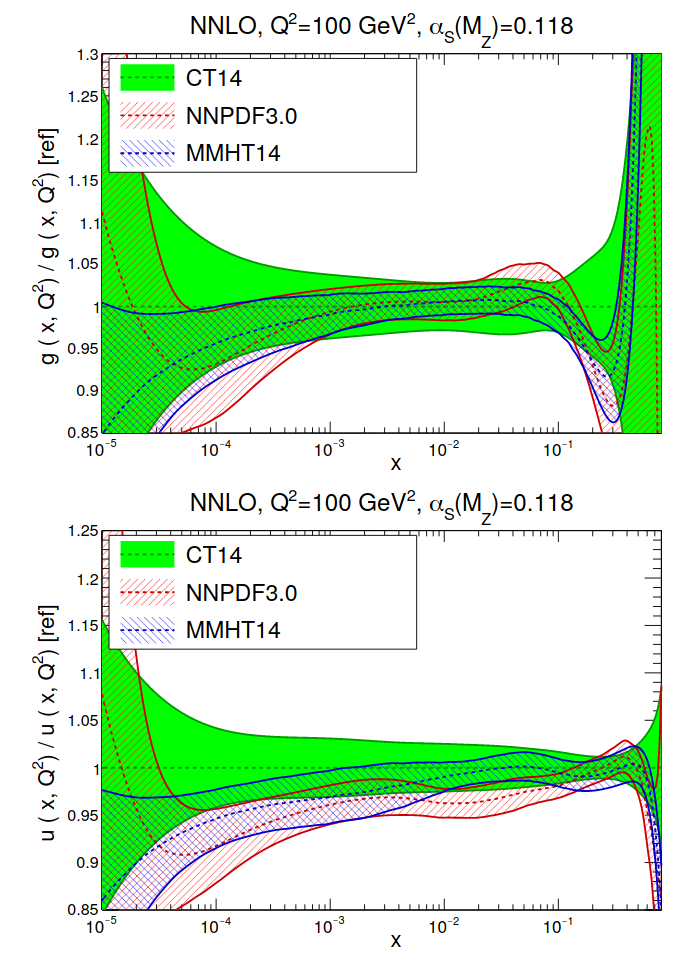
\includegraphics[width=.95\textwidth]{figures/protoncollisions/pdf_comparison.png}
    \caption{Comparison of the gluon (top) and up quark (bottom) PDFs from the CT14, MMHT14 and  NNNPDF3.0 sets at next-to-next-to-leading order (\NNLO) at a scale of \(Q^2= \SI{100}{\square\giga\electronvolt}\). The results are shown relative to the central value of CT14. Figure reproduced from Ref.~\cite{Butterworth2016}.}
    \label{fig:pp:pdfs:comparison}
\end{figure}


\section{Calculation of cross-sections}
\label{sec:pp:crosssections}
According to factorisation theorems~\cite{Collins1989}, the total cross-section for any process \HepProcess{\Pproton \Pproton \to X} can be written as a sum over the partonic cross-sections \(\hat{\sigma}_{\HepProcess{a b \to X}}\) for all parton types \(a\) and \(b\)
\begin{align}
    \sigma_{\HepProcess{\Pproton \Pproton \to X}} = \sum_{a} \sum_{b} \int_{0}^{1} \dd{x_{1}} \int_{0}^{1} \dd{x_{2}} f_{a}(x_1, \muF) f_{b}(x_2, \muF) \hat{\sigma}_{\HepProcess{a b \to X}}(x_{1} p_{1}, x_{2} p_{2}, \muF, \muR).
\end{align}

The PDFs in proton-proton collisions evolve with the factorisation scale \(\muF\) according to the same non-perturbative interactions that give rise to scaling violations in deep inelastic scattering. The renormalisation scale \(\muR\) is another process-dependent quantity, which indicates the scale at which the coupling constants are evaluated. Typical choices for \(\muF\) and \(\muR\) are dictated by one hard scale \(Q^2\) of the process like the mass of an \(s\)-channel resonance of mass \(M\), such that \(\muF = \muR = Q^2 = M^2\).

As the momentum of the partons is distributed according to the PDFs, the centre-of-mass frame of the process is unlikely to coincide with the laboratory frame of reference. In the parton model, one parton has momentum \(p_{z_{1}} = x_{1} \sqrt{s} / 2\) in the detector frame, while the other has the momentum \(p_{z_{2}} = - x_{2} \sqrt{s} / 2\), where \(\sqrt{s}\) is the centre-of-mass energy of the proton-proton-system. In the partonic centre-of-mass frame, the energy of the parton is \(\hat{s} = x_1 x_2 s\) and it has net momentum along the beam axis of \(\hat{p}_{z} = (x_1 - x_2)\).

The partonic cross-section in the limit of massless partons
\begin{align}
    \hat{\sigma}_{\HepProcess{a b \to X}}(x_{1} p_{1}, x_{2} p_{2}, \muF, \muR) = \frac{1}{2\hat{s}} \int \dd{\Phi_{n}} \abs{\mathcal{M}_{\HepProcess{a b \to X}}}^2 (\Phi_{n}, \muF, \muR)
\end{align}
can be evaluated in perturbation theory by calculation of the matrix element \(\mathcal{M}_{\HepProcess{a b \to X}}\) and the \(n\)-parton phase space element
\begin{align}
\dd{\Phi_{n}} = \prod_{i=1}^{n} \left[\frac{\dd{p_i}^{4}}{(2\pi)^4} (2\pi) \delta(p_{i}^{2} - m_{i}^{2}) \Theta(p_{i}^{0})\right] (2 \pi)^4 \delta^{4} (p_{a} + p_{b} - \sum_{i=1}^{n} p_{i}).
\end{align}

The cross-sections of typical processes at (anti-)proton-proton colliders for various centre-of-mass energies \(\sqrt{s}\) are shown in \Cref{fig:pp:crosssections:overview}. The cross-sections have been calculated in perturbative QCD at \NLO and \NNLO using the MSTW2008 PDF set~\cite{Martin2009}. Processes of interest, such as weak gauge boson production or Higgs boson production, or hypothetical dark matter particle production occur with cross-sections which are magnitudes below the total inelastic cross-section in \HepProcess{\Pp\Pp} collisions at a centre-of-mass energy of \SI{13}{\tera\electronvolt} of \SI{78.1 \pm 2.9}{\milli\barn}~\cite{STDM-2015-05}. Consequentially, a resource-efficient description of selected collision events for investigating these processes starts with the hard process and builds up the event from there.

\begin{figure}[htbp]
    \centering
    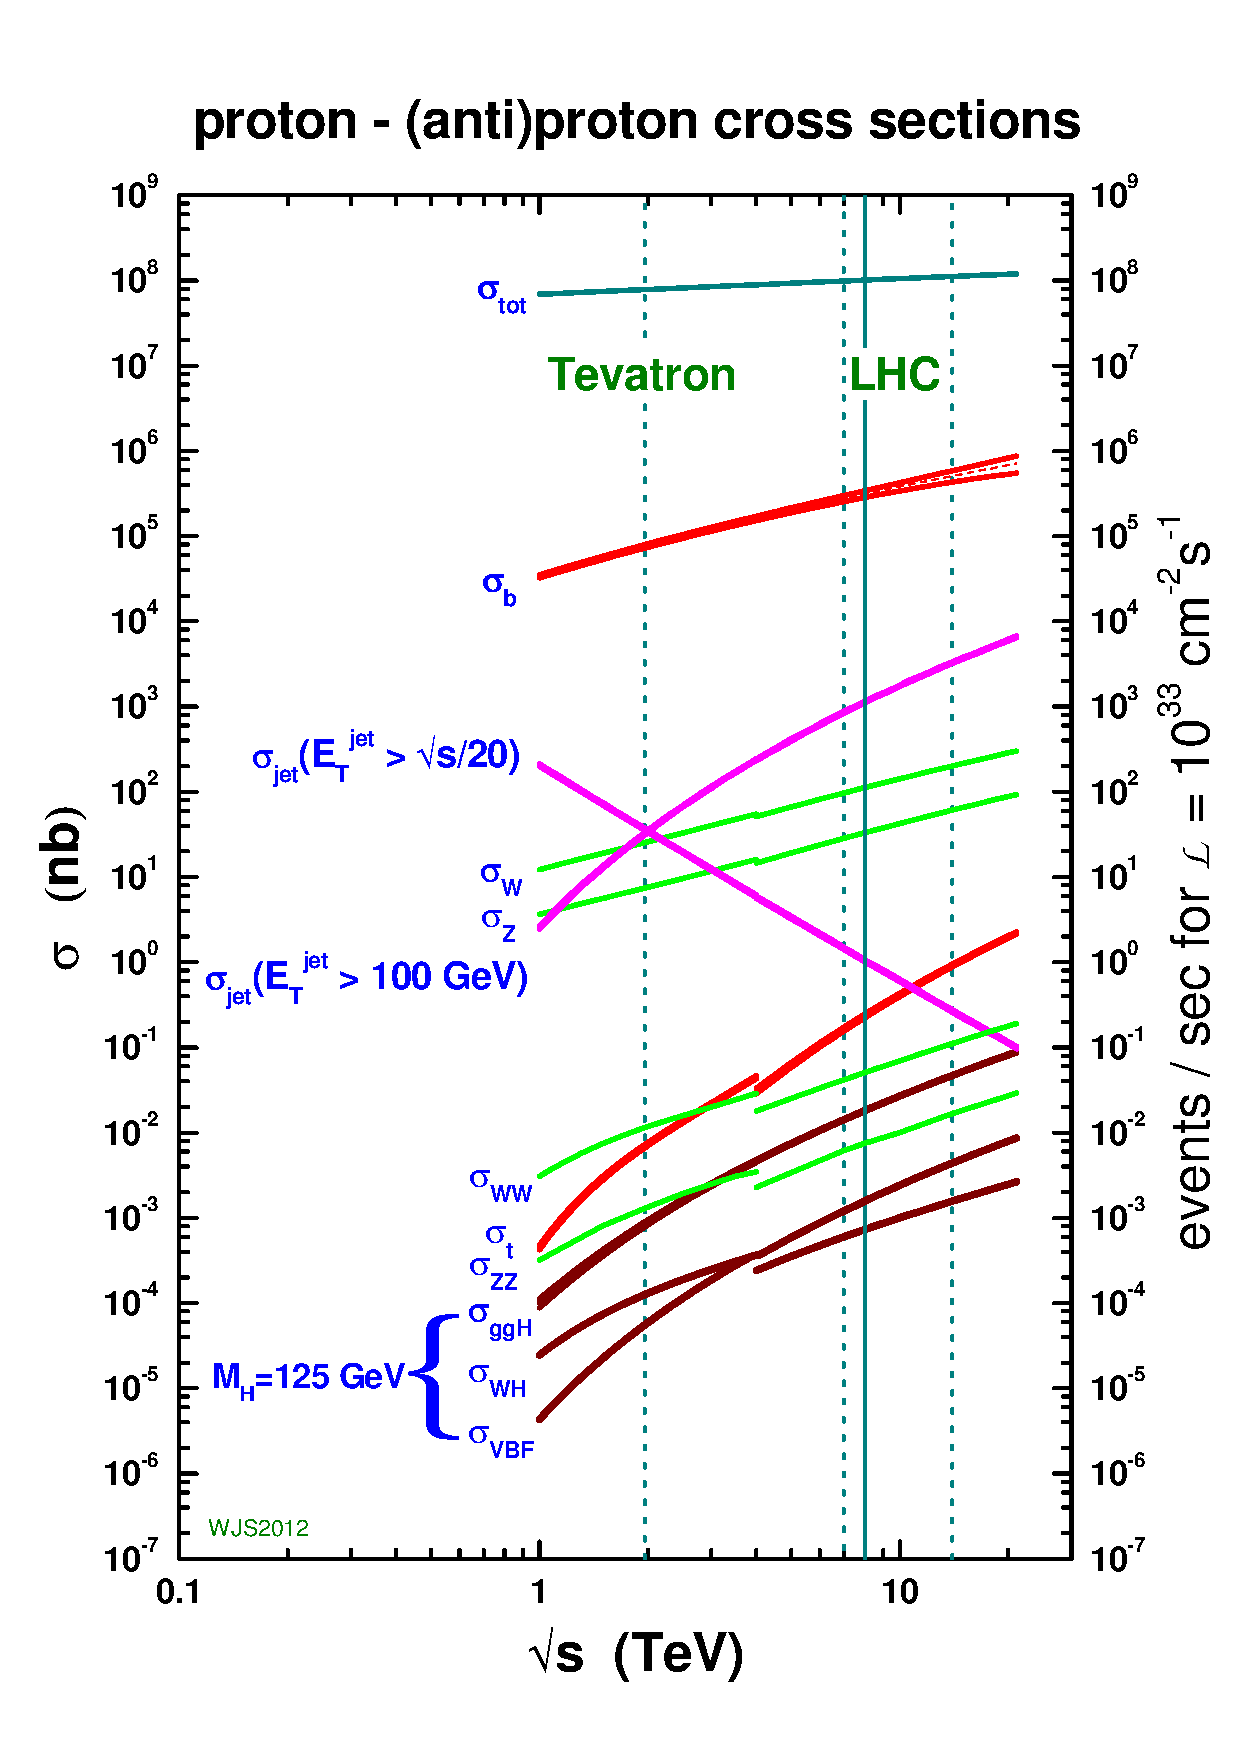
\includegraphics[width=.95\textwidth]{figures/protoncollisions/crosssections2012_v5.pdf}
    \caption{Cross-sections and event rates for various centre-of-mass energies \(\sqrt{s}\) in antiproton-proton (Tevatron, \(\sqrt{s} < \SI{4}{\giga\electronvolt}\)) and proton-proton (LHC, \(\sqrt{s} > \SI{4}{\giga\electronvolt}\)) collisions. The cross-sections have been calculated in perturbative QCD at \NLO and \NNLO using the MSTW2008 PDF set~\cite{Martin2009}. Figure reproduced from Ref.~\cite{Stirling2012}.}
    \label{fig:pp:crosssections:overview}
\end{figure}


\section{Event simulation}
\label{sec:pp:evgen}
The processes of interest in \HepProcess{\Pp\Pp} collisions are simulated by Monte Carlo (MC) event generators~\cite{Buckley2011,Sjostrand2016}.
The matrix elements of the hard scattering process are computed in perturbative QCD at fixed orders in \(\alpha_{s}\) in a highly automated way, together with the corresponding phase-space parametrisations. Event generators describing hard processes are \MGMCatNLO~\cite{Alwall:2014hca} (providing \LO and \NLO accuracy in QCD) and \POWHEG~\cite{Alioli:2010xd} (providing \NLO accuracy in QCD). The PDFs are parametrised in the LHAPDF format~\cite{Buckley2015}.
The secondary emissions are described by parton showers. Potential overlap of the multiple softer emissions of the parton showers and the higher-order matrix elements is resolved by matching and merging prescriptions.

The three general-purpose event generators \SHERPA~\cite{Gleisberg:2008ta}, \HERWIG~\cite{Bellm:2015jjp}, and \PYTHIA~\cite{Sjostrand:2014zea} provide combined descriptions of hard processes interfaced with parton showers. In particular, the \HERWIG and \PYTHIA generators can be interfaced with \MGMCatNLO or \POWHEG to supplement the parton shower description.

Finally, the interactions of final state particles with the ATLAS detector are simulated with the GEANT4~\cite{Agostinelli:2002hh} simulation tool-kit to provide the detector response~\cite{SOFT-2010-01}. The resulting set of simulated collision events is processed in the same manner as observed data with the reconstruction and event selection software.


\section{Hadronic jets}
\label{sec:pp:jets}
The parton shower evolution is dominated by the emission of partons which are either soft or collinear with the outgoing partons. Consequentially, the emerging hadrons are distributed in localised collimated sprays, which are called jets. The intriguing feature of jets is the correspondence between the total momentum of the hadrons contained in a jet and that of the corresponding partons described by perturbative calculations. This correspondence allows inferring the properties of the hard scattering process from the detector signature produced by QCD jets.

Jets are no fundamental objects but are instead defined by a jet algorithm. A jet algorithm provides a prescription on how to construct jets from input objects. Thereby, the algorithms need to fulfil two tasks. First, they need to identify all potential jet constituents. Second, they need to define the jet's four-vector based on the information provided by the constituents. A jet algorithm is agnostic to the precise nature of the input objects as long they can be parametrised as four-vectors. Therefore, the input objects can be partons, hadrons or energy deposits in the detectors.

A jet algorithm must be well-defined in arbitrarily high orders of perturbation theory, which involve additional parton emissions, to allow the direct comparison of perturbative calculations with observations. A well-defined jet algorithm, therefore, needs to satisfy the requirements of collinear and infra-red safety: neither collinear splitting nor soft emissions should alter the result of the jet algorithm.

There are two categories of jet algorithms, which differ in their method of identifying the jet constituents.
Cone-based algorithms, such as thee SISCone algorithm~\cite{Salam2007}, are based on purely geometric considerations by defining a jet axis and associating all objects within a specific radius parameter. Sequential algorithms cluster and combine pairs of objects until all objects have been used.

The \(k_{\text{T}}\) algorithms are a family of sequential algorithms, which satisfy the requirements of collinear and infra-red safety and are successfully employed at the Large Hadron Collider experiments.
They iteratively group objects \(i\) and \(j\) (referred to as pseudo-jets) into jets, using the two generalised distance measures in momentum space between two pseudo-jets (\(d_{ij}\)) and a pseudo-jet and the beam (\(d_{iB}\))
\begin{align}
	d_{iB} &= (\pt)^{2p} \\
    d_{ij} &= \min{\left\{(p_{\text{T}, i})^{2p}, (p_{\text{T}, j})^{2p} \right\}} \times \frac{R_{ij}}{R_{0}},
\end{align}
which are based on the transverse momenta of the pseudo-jets \(p_{\text{T}, i}\) and on the distance between the two objects in the \(\eta\)-\(\varphi\)-plane \(R_{ij} = \sqrt{\Delta\eta^2 + \Delta\varphi^2}\).

The algorithm evaluates all possible \(d_{ij}\) and \(d_{iB}\) and identifies the smallest distance. If the smallest distance is between a pseudo-jet and the beam, the pseudo-jet is promoted to a jet and is added to the list of output objects. Otherwise, the two pseudo-jets are discarded, and a new pseudo-jet \(k\) whose kinematic properties are based on their vector sum is created. This step is repeated until all pseudo-jets have been promoted to jets.

The parameter \(p\) defines the type of jet algorithm in the \(k_{\text{T}}\) family:
\begin{itemize}
	\item \(k_{\text{T}}\) algorithm (\(p = 1\))~\cite{Catani1993,Ellis1993}
	\item Cambridge/Aachen algorithm (\(p = 0\))~\cite{Dokshitzer1997,}
	\item \Antikt algorithm (\(p = -1\))~\cite{Cacciari2008}
\end{itemize}

The jet area can be determined by populating the \(\eta\)-\(\varphi\)-plane of an event with ghost particles, which have infinitely small momentum~\cite{Cacciari2008-2}. As the \(k_{\text{T}}\) algorithms are collinear and infra-red safe, the reconstructed jets are not changed by the addition of ghost particles. However, the association of the ghost particles with jets allows inferring the jet catchment area.

\Cref{fig:pp:jets:algorithms} shows a comparison of the resulting jet areas for the three algorithms of the \(k_{\text{T}}\) family and the SISCone algorithm. The \(k_{\text{T}}\) and Cambridge/Aachen algorithms produce jets with more irregular jet shapes, while the SISCone and \antikt algorithms have more regular jet shapes.

The \antikt algorithm, which is used as the standard jet algorithm in this dissertation, is collinear and infra-red safe and provides jets with a nearly conical shape at excellent reconstruction efficiency. Depending on the use-case, a different radius parameter is used for the jet reconstruction. The jet algorithms are implemented in the FastJet package~\cite{Cacciari2012}.

\begin{figure}[htbp]
    \centering
    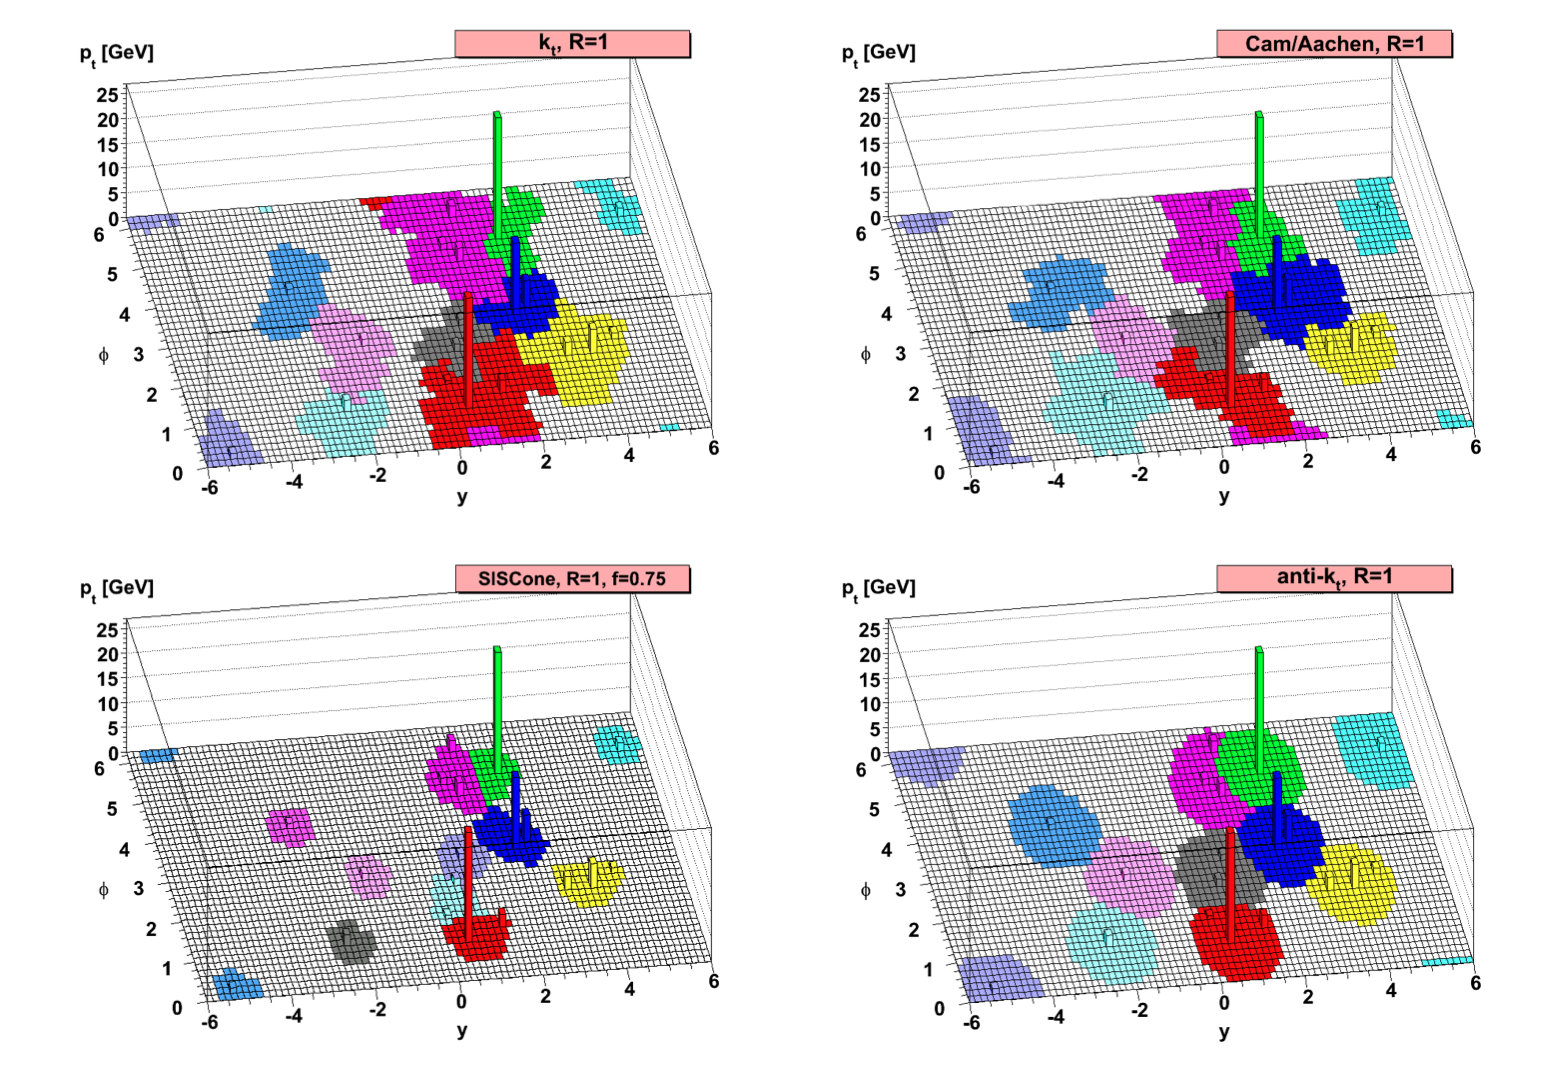
\includegraphics[width=.95\textwidth]{figures/protoncollisions/jetalgorithms.png}
    \caption{Clustering of a sample parton-level event with four different jet algorithms, illustrated by the active catchment area of the resulting hard jets. Figure reproduced from Ref.~\cite{Cacciari2008}.}
    \label{fig:pp:jets:algorithms}
\end{figure}

% % !TEX root = ../my-dissertation.tex
%
\chapter{Experimental apparatus}
\label{sec:experiment}

\section{Introduction}
\label{sec:experiment:introduction}
Scattering experiments have been the key to furthering our understanding of the elementary constituents of matter and their interactions. The seminal work of Geiger, Marsden, and Rutherford~\cite{Geiger_1908} on the scattering of \(\alpha\)-particles%
\footnote{The kinetic energy of the \(\alpha\)-particles used in Rutherford's experiment is \SI{8}{\mega\electronvolt}. Modern particle accelerators achieve millionfold beam energy of \SI{6.5}{\tera\electronvolt}.} %
from thin metal foils in 1908 unravelled the structure of the atom and led to the discovery of the atomic nucleus.
Today, scattering experiments have evolved to using the very same atomic nuclei discovered over a century ago as probes for the uncharted frontiers of particle physics.

The natural observable of scattering experiments is the cross-section \(\sigma\)~\cite{Thomson2013}. In a classical interpretation, the number of scattered objects is related to the cross-sectional area of a scattering object, which allowed Rutherford to deduce the size of the atomic nucleus. However, the quantum nature of elementary particles ultimately only allows for a probabilistic description of nature by predicting the probability for a process to happen. In this interpretation, the cross-section has a more abstract meaning as a measure of the interaction strength. It is related to the underlying theory by the equation~\cite{Schwartz2013}
\begin{align}
    \sigma = \frac{1}{\Phi_{i}} \int \abs{\bra{f} \mathcal{M} \ket{i}}^2 \dd{\Pi}_{f}.
\end{align}
Here, \(\Phi_{i}\) is the flux of initial state particles \(\ket{i}\) and \(\dd{\Pi}_{f}\) is the differential kinematically allowed phase space of the final states \(\ket{f}\). The modulus square of the matrix element \(\bra{f} \mathcal{M} \ket{i}\) gives the probability \(P(\ket{i} \rightarrow \ket{f})\) for a transition from \(\ket{i}\) to \(\ket{f}\). The preparation of initial states \(\ket{i}\) and measurement of final states \(\ket{f}\) dictates the experimental setup of a scattering experiment with the aim of empirically testing the underlying theory and exploring the structure of matter.

The momentum of initial states \(\ket{i}\) determines the scale on which nature can be investigated\footnote{The de Broglie relation \(\lambda = 1 / p\) relates the momentum \(p\) of a probe with the size of the structure that can be resolved.}.
Rays of particles with considerable momentum and consequently smaller wavelength allow probing structures on more minor length scales.
Although cosmic rays from astrophysical sources can achieve ultra-relativistic energies up to \SI{e20}{\electronvolt}, their rate is vanishingly small~\cite{Gaisser2016}, so that one can only hope for their detection by terrestrial experiments.

The invention of modern particle accelerators marked a turning point. Particle accelerators not only allow for a reproducible preparation of initial states \(\ket{i}\) in a controlled laboratory environment but also their production in abundant number.
Remarkably, the kinetic energy of colliding particles also determines the mass scale of the particles created in the collision, possibly giving access to previously inaccessible heavy states. As their production cross-section often is small, only particle accelerators can produce these heavy states in sufficient quantities to allow for their observation.
In summary, in a modern scattering experiment, particle accelerators prepare the initial states \(\ket{i}\).
The two defining quantities of equal importance for a collider experiment are the energy and the rate of collision events.
The total beam energy in the centre-of-mass frame \(\sqrt{s}\) is the first defining characteristic of particle accelerators. High centre-of-mass energy is required for probing the structure of matter at smallest scales and for producing yet unobserved heavy states.
The luminosity is the second defining characteristic of a collider experiment. The number of scattering events measured in a collider experiment for a process with cross-section \(\sigma\) during a time \(\Delta T\) is
\begin{align}
    N =  \sigma \cdot \int\limits_{\Delta T} \dd{T} L_{\text{inst}} = \sigma \cdot L.
\end{align}
It is determined by the instantaneous luminosity \(L_{\text{inst}}\).  The amount of collected data is quantified by the integrated luminosity \(L\), typically stated in the unit \(\si{\per\femto\barn}\)\footnote{Cross-sections are stated in units of length-squared as multiples of a barn, with \(\SI{1}{\barn}=\SI{e-28}{\square\meter}\). The whimsical name owes its creation to physicists of Purdue University. They associated the typical cross-sectional size of a \ch{U} atomic nucleus with the dominant feature of Midwestern farmlands, which is referred to by the idiom ``you can’t hit the side of a barn''.}.

Particle detectors measure properties of final states \(\ket{f}\). To this end, they typically employ three specific types of detector subsystems situated in the increasing distance to the interaction point.
First, tracking detectors immersed in magnetic fields provide precision position and momentum-measurements of charged particles. Second, calorimeters measure the energy deposited by electrons, photons, and hadrons. Finally, muon detectors measure the path and momentum of muons passing the calorimeter.

From this discussion, three experimental design requirements for dark matter searches become evident.
\begin{enumerate}
    \item Processes resulting in the production of dark matter particles at a collider experiment are expected to occur with minute cross-sections at the order of \(\mathcal{O}(\si{\femto\barn})\). Also, dark matter production might involve heavy states which are only accessible with sufficient beam energy above their production threshold. Consequently, the exploration of terrestrial dark matter production in a laboratory requires a particle accelerator with both high beam energy and high beam intensity.
    \item A \HepProcess{\Pp\Pp} machine is the optimal choice for probing dark matter in collider experiments. Although the models for the production of dark matter particles discussed in \Cref{sec:dm:models} specify the type and interactions of the new states they predict, they make no exact predictions about their mass. Searches for dark matter are required to be sensitive to new physics across a large mass range. To this end, the use of composite objects, such as protons, as initial states allows probing a wide range of possible new heavy states at a fixed collision energy \(s\). As only the partons and not the entire proton participate in the hard scattering process, the effective centre-of-mass energy of the interaction \(s' = x_a \cdot x_b \cdot s\) depends on the momentum fractions \(x_a\) and \(x_b\) of the initial state partons. As a result, the energy available for the resonant production of new particles is not fixed as it is the case for electron-positron colliders, making hadron colliders powerful discovery machines.
    \item Once produced, dark matter particles do not interact with detector material. They can only be observed via their recoil on other particles, which results in a missing component \(E^{\text{miss}}\) in the observed energy-momentum balance of the collision. Therefore, an ideal detector for dark matter searches must not only reconstruct all types of physics objects with excellent precision but also provide hermetical \(4\pi\) coverage in full solid angle.
\end{enumerate}

These requirements are met by the Large Hadron Collider (LHC) and the ATLAS detector at the European Organisation for Nuclear Research CERN. Section~\ref{sec:experiment:LHC} explores the LHC as the culminating part of the CERN accelerator complex and gives an overview of its operation parameters during the years 2015 to 2018. The discussion of the ATLAS detector and its subsystems is provided in Section~\ref{sec:experiment:ATLAS}.


\section{The Large Hadron Collider}
\label{sec:experiment:LHC}
The Large Hadron Collider (LHC)~\cite{Evans2008} is, at the time of writing, the most powerful terrestrial particle accelerator. Its approximately circular geometry extends \SI{26.7}{\kilo\meter} in circumference. The LHC is located in the tunnel which formerly hosted the Large Electron-Positron (LEP) collider and lies \SIrange{75}{175}{\meter} below the surface of the Franco-Swiss border at CERN near Geneva.
The LHC is designed to accelerate and collide two counter-rotating beams of protons in an ultra-high vacuum with a maximum centre-of-mass energy of \(\sqrt{s} = \SI{14}{\tera\electronvolt}\). During Run-1 operation during \numrange{2009}{2013} at centre-of-mass energies of \(\sqrt{s} = \SI{7}{\tera\electronvolt}\) and \SI{7}{\tera\electronvolt}. This dissertation is based on data taken during Run-2 operation in 2015 to 2018, where the LHC was operated at the centre-of-mass energy of \(\sqrt{s} = \SI{13}{\tera\electronvolt}\) and at peak luminosity of \SI{2.1e34}{\per\square\centi\meter\per\second}. Although the LHC's design also allows for colliding heavy lead ions with an energy of up to \SI{2.8}{\tera\electronvolt} per nucleon, heavy ion physics is beyond the scope of this dissertation and only the proton physics programme is briefly discussed in the following. A more detailed account is given in Refs.~\cite{Bruning2004v1,Bruning2004v2,Benedikt2004}.

The protons injected to the LHC undergo several stages of acceleration in a pre-accelerator-chain~\cite{Benedikt2004}, shown in \Cref{fig:LHC-chain}.

\begin{figure}[htbp]
    \centering
    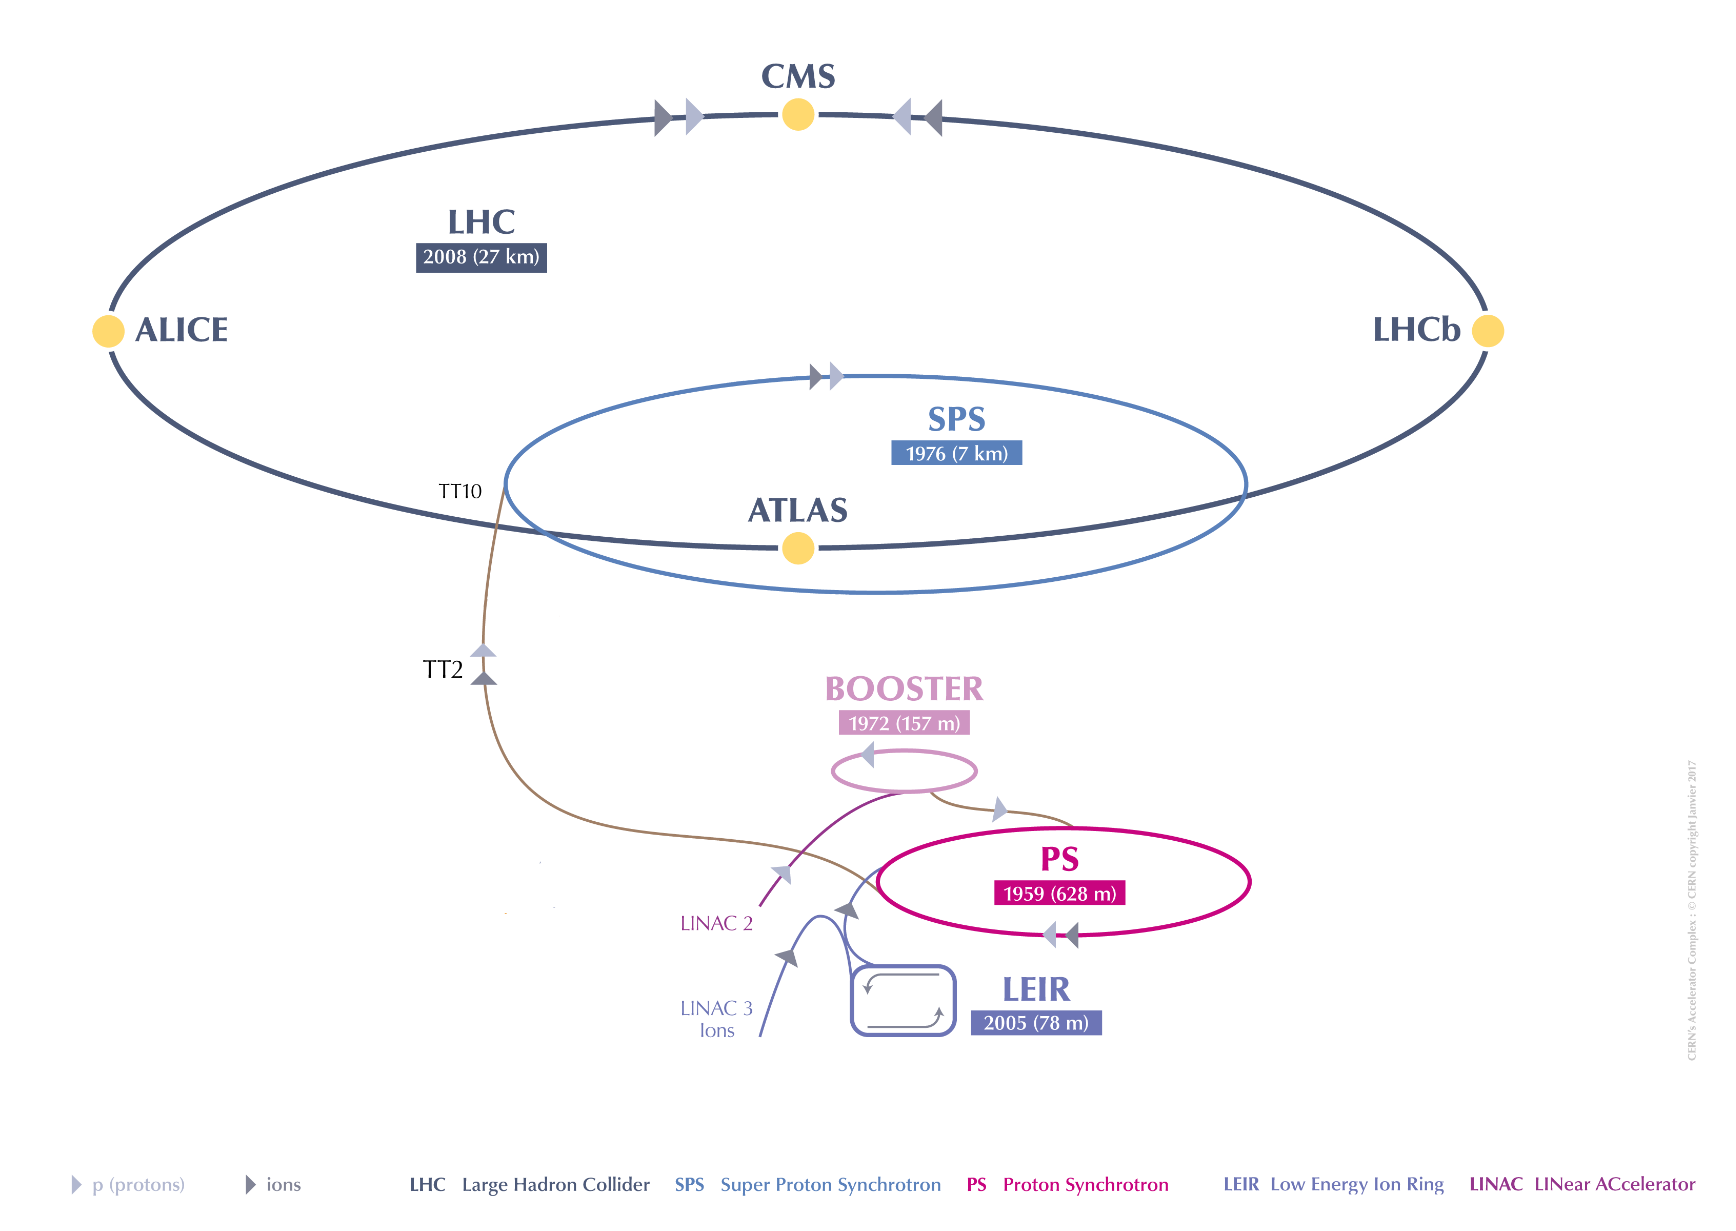
\includegraphics[width=0.95\textwidth]{figures/experiment/cernaccelerators.png}
    \caption{The CERN accelerator complex. The illustration shows the LHC ring and the associated pre-accelerator chain relevant for producing \HepProcess{\Pp\Pp} collisions. Figure adapted from Ref.~\cite{Mobs:2197559}.}
    \label{fig:LHC-chain}
\end{figure}

They start their journey as hydrogen atoms, supplied from a simple gas bottle and ionised by stripping them of their electrons in a duoplasmatron machine~\cite{Bailey2014}.
The protons emerge as a beam with \SI{300}{\milli\ampere} current and are first accelerated to \(\sqrt{s} = \SI{50}{\mega\electronvolt}\) by the LINAC2 linear accelerator.
The Proton Synchroton Booster (PSB) and the Proton Synchrotron (PS) perform the next acceleration stages. Both are synchrotron accelerators. The PSB consists of four synchrotron rings with a radius of \SI{25}{\meter}, which are stacked on top of each other, and accelerates the protons to \(\sqrt{s} = \SI{1.4}{\giga\electronvolt}\). The PS extends over large parts of the CERN Meyrin site with a radius of \SI{100}{\meter} and raises the beam energy to \SI{25}{\giga\electronvolt}. As each of the four PSB rings extends one-quarter of the PS circumference, the PSB beam can be extracted sequentially to the PS. As the beams are extracted and injected by kicker magnets, pulsed dipole magnets with swift time response, they arrive not continuously but in discrete bunches.
The Super Proton Synchrotron, extending \SI{7}{\kilo\meter} in circumference, ramps up the beam energy to \SI{450}{\giga\electronvolt} before the proton beams are injected in the two storage rings of the LHC.

In the LHC, particles are accelerated by radio frequency (RF) cavities driven by high power klystrons. The RF system is operated at \SI{400.79}{\mega\hertz} with each cavity providing a field gradient of \SI{5.5}{\mega\volt\per\meter} and \SI{2}{\mega\electronvolt} acceleration voltage, resulting in a total increase of the beam energy by \SI{485}{\kilo\electronvolt} per revolution.

The LHC beams are kept on their circular trajectories by \num{1232} superconducting niobium-titanium dipole magnets operated at a temperature of \SI{1.9}{\kelvin} with magnetic field strengths of \SI{8.33}{\tesla}. The space constraints imposed by the tunnel require a twin-bore magnet design, hosting the two beam pipes and two sets of magnet coils within the same mechanical structure and cryostat. The beams are focussed using quadrupole and higher-order multipole magnets.

The machine luminosity is determined by several beam parameters, which are listed in \Cref{tab:lhcparameters}, and can be written as
\begin{align}
    L = \frac{N_{b}^2 n_b f_{\text{rev}} \gamma_r F}{4 \pi \varepsilon_n \beta^{*}}.
\end{align}

The luminosity is determined by in-situ measurements performed with dedicated detectors and van-der-Meer scans~\cite{vanderMeer:296752,ATLAS-CONF-2019-021}.

\begin{table}
\caption{Essential LHC parameters with their description and values during Run-2 operation~\cite{Evans2008}.}
\label{tab:lhcparameters}
\resizebox{1.0\textwidth}{!}{%
\begin{tabular}{llr}
\toprule
Parameter & Description & Value \\
\midrule
\(E\) & beam energy & \SI{6.5}{\tera\electronvolt} \\
\(L_{\text{inst}}\)& peak luminosity & \SI{2e34}{\per\square\centi\meter\per\second}\\
\(N_b\) & particles per bunch& \num{1.15e11} \\
\(n_b\) & bunches per beam & \num{2808} \\
\(f_{\text{rev}}\) & revolution frequency & \SI{11.245}{\kilo\hertz} \\
\(\gamma\) & relativistic gamma factor & \num{7461} \\
\(\varepsilon_n\) & normalised transverse beam emittance & \SI{3.75}{\micro\meter}\\
\(\beta^{*}\) & \(\beta\) function at collision point & \SI{0.5}{\meter}\\
\multirow{2}{*}{\(F\)} & geometric luminosity reduction factor & \multirow{2}{*}{\num{0.836}}\\
& due to crossing angle at interaction point & \\
\bottomrule
\end{tabular}}
\end{table}

The two beams intersect at four interaction points, each within a cavern hosting one of the four extensive LHC experiments ATLAS~\cite{ATLAS2008}, LHCb~\cite{LHCB2008}, CMS~\cite{CMS2008}, and ALICE~\cite{ALICE2008}.
In total, there are eight LHC experiments. The three smaller experiments, TOTEM~\cite{TOTEM2008}, LHCf~\cite{LHCF2008}, MoEDAL~\cite{Mitsou2017}, and FASER~\cite{Ariga:2651328}, complement the LHC physics programme by more specific measurements. TOTEM and LHCf use detectors positioned close to the CMS and ATLAS experiment, respectively, to investigate the physics of particles generated almost directly in line with the colliding proton beams. The prime goal of the MoEDAL experiment, which shares the cavern with LHCb, is the search for magnetic monopoles and exotic particles.
The FASER experiment, which is located in a service tunnel downstream from the interaction point used by the ATLAS experiment, searches for light, weakly-coupled particles and investigates the interactions of high-energy neutrinos.
The LHCb experiment is a specialised detector investigating flavour physics. The ALICE experiment investigates physics of strongly interacting matter at extreme energy densities by analysing heavy lead ion collisions. The two all-purpose detectors ATLAS and CMS, operated at peak luminosity, are located in opposed caverns. Their independent operation and different detector design are crucial for cross-checks and reciprocal corroboration in the event of a potential discovery.

Although high beam intensities enhance searches for rare processes by increasing the collected data over time, they also increase the number of simultaneous \HepProcess{\Pp\Pp} interactions in a single collision event. Such multiple \HepProcess{\Pp\Pp} interactions are known as pile-up and are typically uncorrelated with the hard-scattering process. Therefore, they contribute a largely diffuse background of primarily soft energy depositions in the detector. One distinguishes between in-time pile-up, which refers to multiple collision events within the same bunch crossing, and out-of-time-pileup, which refers to energy deposits from previous and following bunch crossings concerning the triggered event. The total expected amount of pile-up \(\mu\) is related to the instantaneous luminosity by the equation
\begin{align}
    \mu = \frac{\mathcal{L} \sigma_{\text{inel}}}{N_b n_b f_{\text{rev}}},
\end{align}
where \(\sigma_{\text{inel}} = \SI{78.1 \pm 2.9}{\milli\barn}\) is the inelastic \HepProcess{\Pp\Pp} cross-section~\cite{STDM-2015-05}.


\section{The ATLAS detector}
\label{sec:experiment:ATLAS}
The ATLAS detector is a multi-purpose detector for recording collisions at the LHC. Its design is influenced by both the extreme conditions at the LHC and by the requirements for precision measurements and potential discovery of new physics processes at the \si{\tera\electronvolt} scale.
The high interaction rates and radiation doses delivered to LHC detectors require fast, radiation-hard electronics and detector elements with high granularity. The demands for performing high precision tests of quantum chromodynamics,  exploring the mechanism of electroweak symmetry breaking, and searching for signatures of new physics phenomena dictate the design of the detector and its subsystems.

The ATLAS detector has a cylindrical geometry and extends \SI{44}{\meter} in length and \SI{25}{\meter} in diameter with a weight of \SI{7000}{\tonne}. A sketch of the ATLAS detector, highlighting its various subsystems, is provided in \Cref{fig:ATLAS-full}.

\begin{figure*}[htbp]
    \centering
    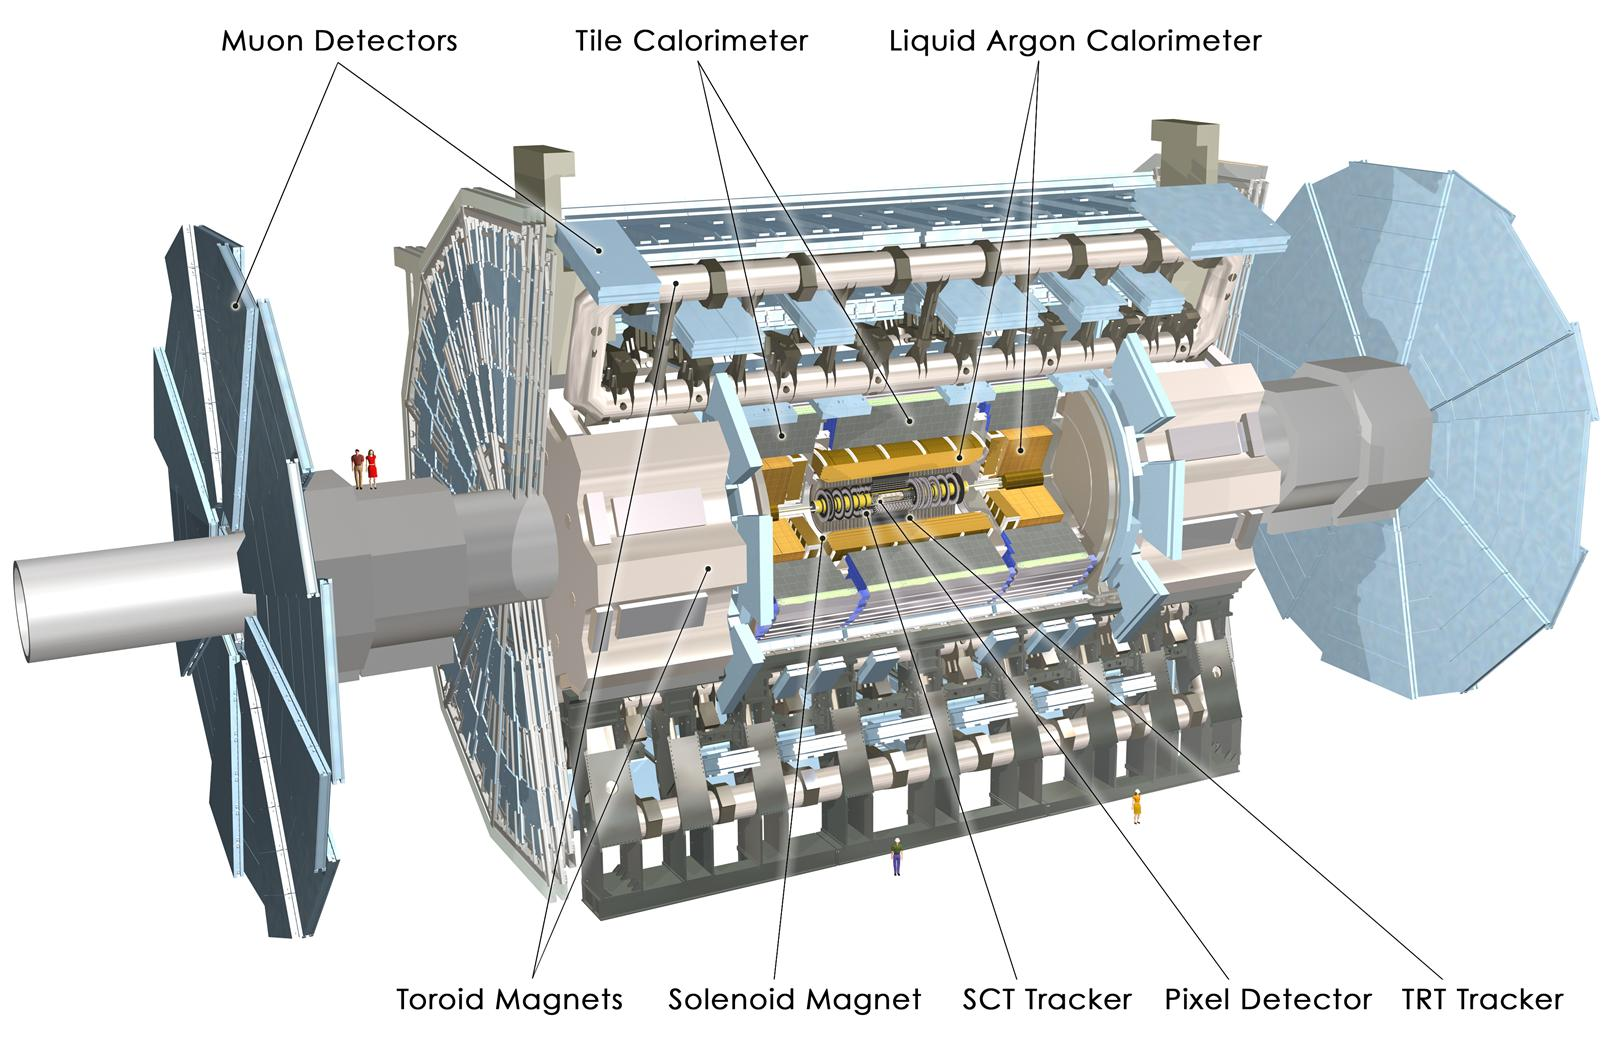
\includegraphics[width=0.95\textwidth]{figures/experiment/detector_full.jpg}
    \caption{Schematic representation of the ATLAS detector and its various subsystems. Figure reproduced from Ref.~\cite{ATLAS2008}.}
    \label{fig:ATLAS-full}
\end{figure*}

The detector consists of a cylindrical barrel region and two wheel-shaped end-caps, each instrumented with detector subsystems to achieve full coverage in the full \(4\pi\) solid angle. The detector geometry possesses an eightfold symmetry around the beam axis and a forward-backwards symmetry to the interaction point.
The detector is comprised of three main subsystems, starting with the innermost component, the inner detector, calorimeters and muon spectrometer. They are introduced briefly in the following. A detailed description of the ATLAS detector is provided in Ref.~\cite{ATLAS2008}.
\subsection{The ATLAS coordinate system}
The ATLAS coordinate system is used throughout this dissertation and defined by expressing space-time events in terms of a right-handed Cartesian coordinate system with its origin located at the nominal interaction point.
The \(z\)-axis is defined by the beam axis, the positive \(x\)-axis points from the interaction point to the centre of the LHC ring, and the positive \(y\)-axis points towards the earth's surface.
The symmetry of the experiment favours a cylindrical coordinate system with the azimuthal angle \(\varphi\) measured around the beam axis and the polar angle \(\theta\) measured from the beam axis.
In collider experiments, it is common practice to express the inclination of a particle with four-momentum \(p = (E, \vec{p})\) to the beam with the pseudorapidity
\begin{align}
    \eta = - \ln \tan{\frac{\theta}{2}} = \frac{1}{2} \cdot \ln{\frac{\abs{\vec{p}} + p_z}{\abs{\vec{p}} - p_z}}.
\end{align}
The pseudorapidity is zero in transverse direction and increases rapidly for smaller inclinations with respect to the beam axis.
In the relativistic limit, the pseudorapidity approaches to the rapidity
\begin{align}
    y = \frac{1}{2} \cdot \ln{\frac{E + p_z}{E - p_z}}.
\end{align}
The phase-space measure of a particle \(\dd{\Pi}_{f}\) is proportional to the rapidity, thus the particle flux per rapidity interval is approximately constant.
Differences in rapidity (and by extension also the pseudorapidity) are invariants under Lorentz boosts along the beams axis. As a consequence, measurements of rapidity differences \(\Delta y\) between particles are the same in different reference frames connected by a Lorentz boost along the beam axis. An invariant distance measure can be defined in the pseudorapidity-azimuthal angle space as
\begin{align}
    \Delta R = \sqrt{\Delta \eta^2 + \Delta \varphi^2} = \sqrt{(\eta_1 - \eta_2)^2 + (\varphi_1 - \varphi_2)^2}.
\end{align}
The composite nature of the colliding protons only allows specifying the transverse momentum component of initial state partons taking part in the hard-scattering process. The aforementioned property of the rapidity therefore is crucially important for interpreting measurements of particles created in \HepProcess{\Pp\Pp} collisions. In a similar vein, it is useful to define transverse quantities of observables, such the transverse momentum
\begin{align}
    p_{\text{T}} = \abs{\vec{p}} \sin{\theta} = \abs{\vec{p}} \cosh{\eta}
\end{align}
which is the projection of the momentum \(p\) onto the \(x\)-\(y\) plane.
Similarly, the missing transverse momentum component in the \(x\)-\(y\) plane \(E_{\text{T}}^{\text{miss}}\) is of particular importance for dark matter searches.
Other variables to describe the trajectory of a particle are the transverse impact parameter \(d_0\) and the longitudinal impact parameter \(z_0\). These are defined as the closest distance between the particle's trajectory and the reconstructed primary vertex in the transverse plane or longitudinal \(z\)-direction, respectively.


\subsection{Magnet system}
\label{sec:experiment:ATLAS:magnets}
Momentum and charge measurement of charged particles requires the bending of their trajectories by being immersed in magnetic fields. To this end, ATLAS is equipped with a magnet system consisting of four large superconducting magnets. All magnets employ superconducting niobium-titanium technology and are cooled to about \SI{4.5}{\kelvin} using liquid helium-3. The energy stored in the ATLAS magnets during operation amounts to \SI{1.6}{\giga\joule}.
The central solenoid magnet is aligned on the beam pipe and provides a \SI{2}{\tesla} axial magnetic field for charged particle measurements in the inner detector. It extends over \SI{5.3}{\meter} length and has a diameter of \SI{2.5}{\meter}. As the magnet is situated between tracking and calorimetry system, a large material budget would impact the calorimeter resolution. The solenoid assembly contributes roughly \num{0.66} radiation lengths at normal incidence, realised by an extremely light-weight structure and shared cooling elements of the solenoid and the calorimeter system.
The barrel toroid and two end-cap toroids are defining for the ATLAS experiment as they not define the name of the experiment but also shape the total dimensions of the detector. The barrel toroid consists of eight air-core race-track shaped coils with an overall length of \SI{25.3}{\meter} covering the region in between \SIrange{9.4}{20.1}{\meter} from the interaction region.
The end-cap toroids are octagonal wheels equipped with eight flat, square toroidal coil units and eight keystone wedges.
Together, the toroids provide toroidal magnetic fields of approximately \SI{0.5}{\tesla} and \SI{1.0}{\tesla} for the muon detectors in the central and the end-cap regions, respectively. The highly non-uniform toroidal field requires a high-precision field mapping by approximately \num{1800} Hall sensors distributed throughout the spectrometer volume.

\subsection{Inner Detector}
\label{sec:ATLAS-ID}
The inner detector provides precision measurements of charged particle trajectories. As it is immersed in the \SI{2}{\tesla} solenoid magnetic field, the track curvature can be used for determining the track's transverse momentum \(p_{\text{T}}\).
The reconstructed particle tracks are used for pattern recognition to identify common points of origin, which are called vertices. The primary vertex is the vertex with the highest scalar \(p_{\text{T}}\) sum of associated tracks satisfying transverse and longitudinal impact parameter requirements. The primary vertex corresponds to the hardest interaction in the event, which typically is the interaction of interest. Other vertices in the same bunch crossing can be used to identify signatures associated with pile-up. Additionally, secondary vertices, which correspond to the displaced decays of short-lived particles, are used to identify the production of \(b\)-quarks or \(\tau\) leptons.
To this end, the inner detector is located close to the interaction region. It is comprised of discrete, high-resolution semiconductor pixel and strip detectors in the inner part of the tracking volume and straw tube tracking detectors in the outer part, with additional capability for particle identification by generating and detecting transition radiation. An essential design requirement is a light material budget to reduce energy losses in the ID.
The momentum resolution of the inner tracker for trajectories of particles with transverse momentum \(p_{\text{T}}\)is approximately
\begin{align}
    \frac{\sigma(p_{\text{T}})}{p_{\text{T}}} = \sqrt{\left(0.05 \% \cdot \left(\frac{p_{\text{T}}}{\si{\giga\electronvolt}}\right)\right)^2 + \left(1 \%\right)^2}.
\end{align}
The layout of the inner detector is illustrated in \Cref{fig:innerdetector}.

\begin{figure}[htbp]
\begin{subfigure}{1.\textwidth}
  \centering
  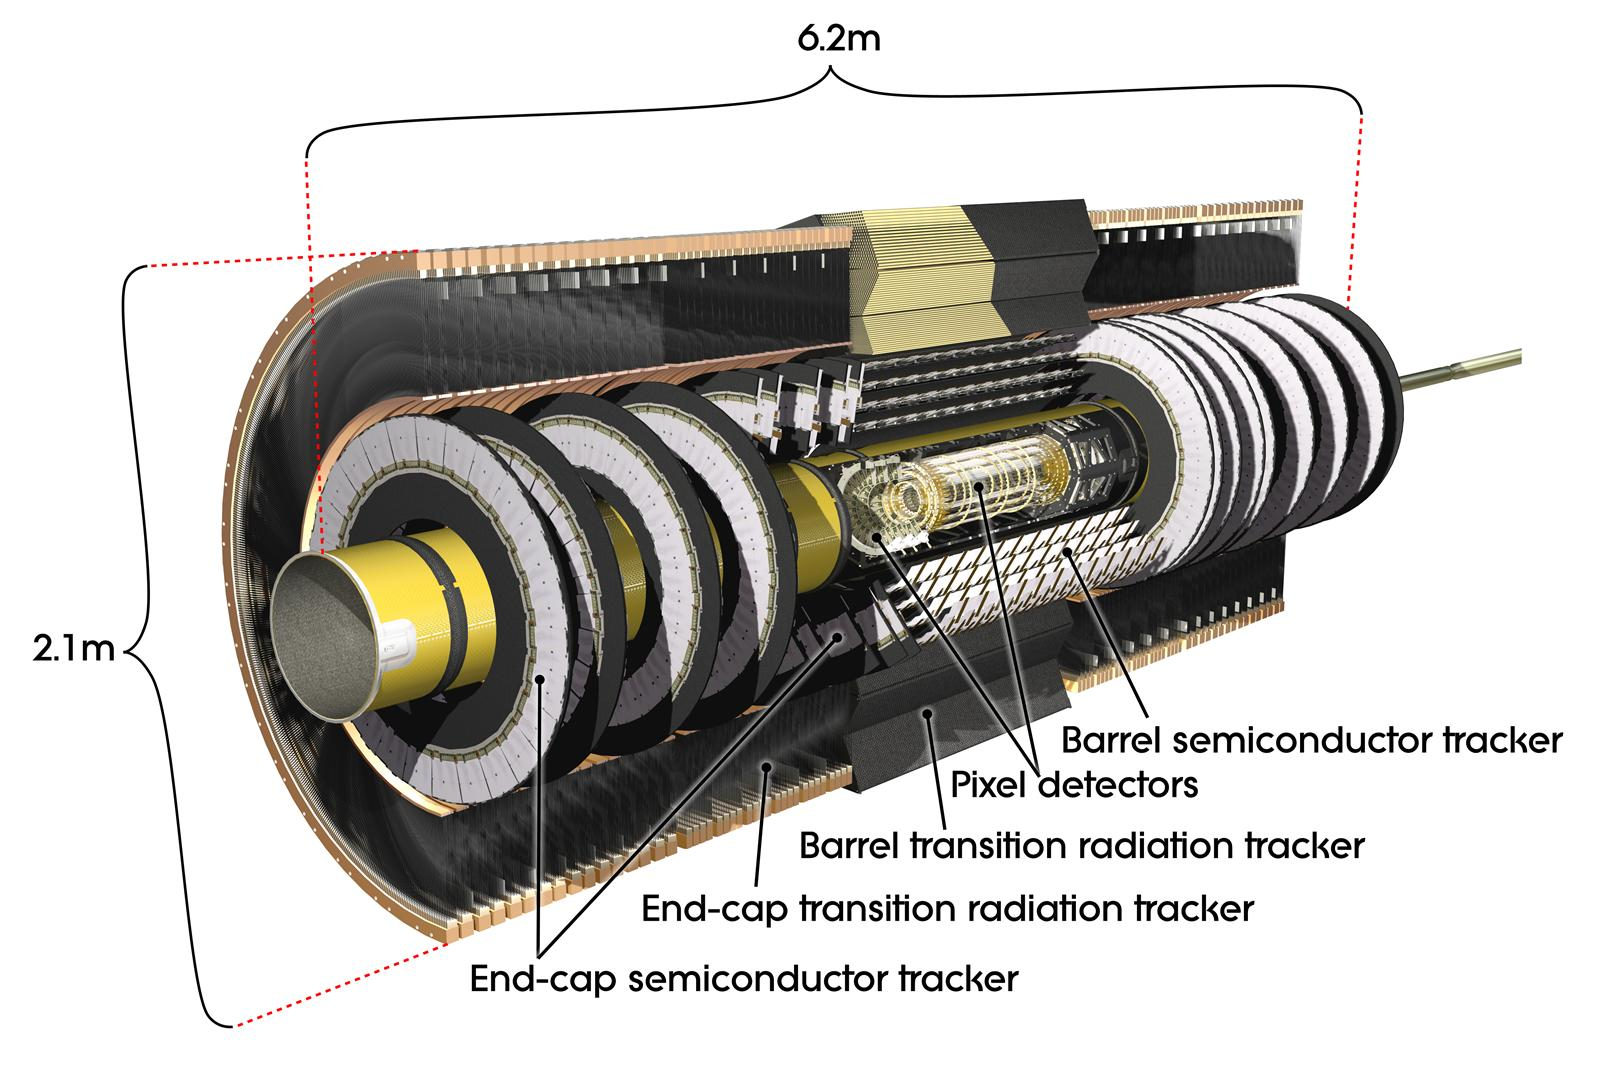
\includegraphics[width=0.95\textwidth]{figures/experiment/innerdetector_full.jpg}
  \caption{Overview of the ID and its sub-detectors. Figure reproduced from Ref.~\cite{ATLAS2008}.}
  \label{fig:innerdetector-full}
\end{subfigure}
\\
\begin{subfigure}{1.\textwidth}
  \centering
  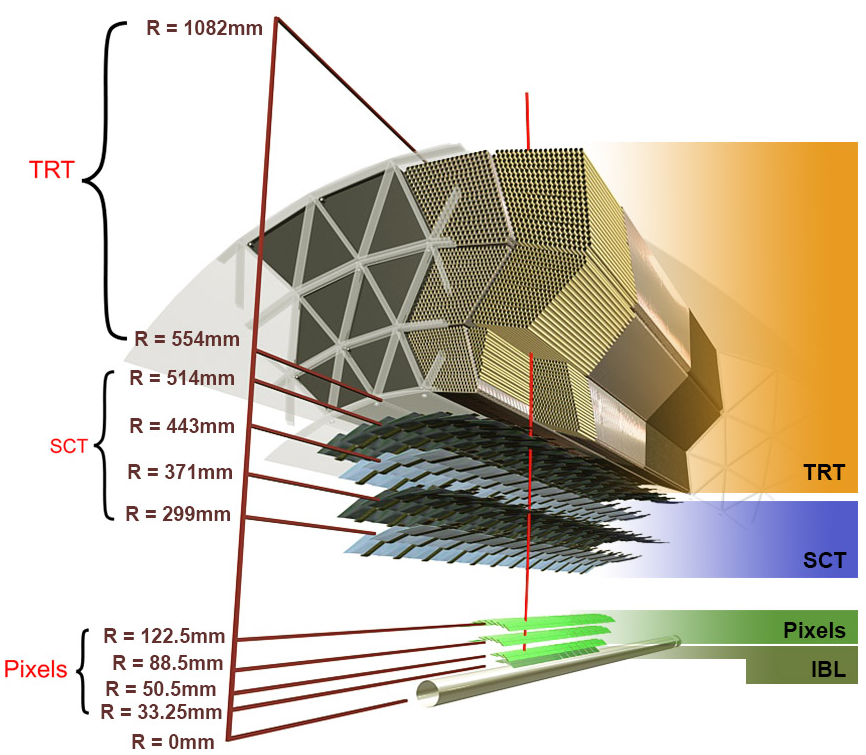
\includegraphics[width=.95\textwidth]{figures/experiment/innerdetector_detail.png}
  \caption{Detailed layout of the ID traversed by a charged track in the barrel region at \(\eta = 0.3\). The track traverses the beam pipe, the four cylindrical PXD layers, the four SCT layers, and approximately 36 axial straws contained within the TRT modules. Figure reproduced from Ref.~\cite{Potamianos:2016ptf}.}
  \label{fig:innerdetector-detail}
\end{subfigure}
    \caption{Illustrations of the ID layout and its spatial dimensions.}
    \label{fig:innerdetector}
\end{figure}

The silicon pixel detector (PXD) is located closest to the beam axis in \SI{12}{\centi\meter} radial distance. Four layers of silicon pixel modules with \num{8.4e7} readout channels provide accurate three-dimensional information with the highest granularity.
In the barrel region, the detector modules are arranged on four concentric cylinders around the beam axis positioned at radii of \SI{33.25}{\milli\meter}, \SI{50.5}{\milli\meter}, \SI{88.5}{\milli\meter}, and \SI{122.5}{\milli\meter}, while in the end-cap regions they are located on six disks perpendicular to the beam axis at distances \(\pm\SI{495}{\milli\meter}\), \(\pm\SI{580}{\milli\meter}\), and \(\pm\SI{650}{\milli\meter}\) from the collision point.
The innermost barrel module, the insertable \(b\)-layer (IBL)~\cite{Abbott2018,CERN-LHCC-2010-013,CERN-LHCC-2012-009}, substantially contributes to the high precision impact parameter measurements, which are critical for vertex identification, by its proximity to the beamline and high spatial resolution.
The PXD provides typically four measurement points for charged particles originating in the beam-interaction region with \SI{10}{\micro\meter} spatial resolution in the transverse plane and \SI{115}{\micro\meter} in the longitudinal \(z\)-direction.

The silicon microstrip tracker (SCT) forms the middle layer of the ID and extends up to \SI{52}{\centi\meter} in the radial distance. As it is located further away from the beamline than the PXD, coarser granularity achieved by \num{6.3e6} readout channels is sufficient. It consists of four concentric layers of silicon strip detectors in the barrel region and 18 wheel-shaped disks containing the sensor modules in the end-cap regions.
Each module hosts two single-sided silicon micros-trip sensor plates rotated about a stereo angle of \SI{40}{\milli\radian} to enable two-dimensional position measurements.
The two precision semiconductor tracking detectors cover the region \(\abs{\eta} < 2.5\). They are connected to a cooling system to reduce noise after irradiation. Their alignment is monitored by comparing positions of module hits with intersections of reconstructed tracks with the modules. Additionally, the SCT alignment is monitored by an interferometry system.
The SCT provides typically eight hits per track at intermediate radii with \SI{17}{\micro\meter} spatial resolution in the transverse plane and \SI{580}{\micro\meter} in the longitudinal \(z\)-direction.

The transition radiation tube tracker (TRT) constitutes the outermost layer of the ID and operates with \num{3.4e5} readout channels. The TRT employs proportional drift tube arrays made of polyimide for track measurements. The choice of drift tubes as detector technology not only allows for the instrumentation of a large volume at comparably low cost but also avoids cooling issues and supports maintaining a low material budget for the ID.
The tubes with diameter of \SI{4}{\milli\meter} contain a \SI{30}{\micro\meter} gold-plated tungsten wire in their centre and are filled with a (\SI{70}{\percent} \ch{Xe} / \SI{27}{\percent} \ch{CO2} / \SI{3}{\percent} \ch{O2}) gas mixture\footnote{As gas leaks occurred during operation of the TRT, some of the TRT modules instead contain an \ch{Ar}-based gas mixture. The presence of this gas mixture is taken into account in the simulation, and the reduced efficiency of \ch{Ar} is partially mitigated by dedicated reconstruction algorithms.}. The tubes are kept at the negative voltage of \SI{1530}{\volt} with their wire kept at ground. The resulting electric field accelerates particles traversing the tubes, which then ionise the gas mixture. As a result, the ionisation products drift to the respective electrode of opposite polarity. Near the wire anode, the field strength is sufficiently high for the electron to create an avalanche of new ionisation processes, manifesting in a signal proportional to the number of primary charges. This measurement determines the primary electron drift time. Based on the knowledge of the drift velocity of electrons in the gas mixture, the radius of the closest approach between the particle trajectory and the wire can be computed. Combining measurements from several individual drift tubes allows determining the particle trajectory unambiguously.
The TRT covers the region \(\abs{\eta} < 2.0\). It provides typically \num{35} hits per track with \(p_{\text{T}} > \SI{0.5}{\giga\electronvolt}\) with \SI{130}{\micro\meter} spatial resolution in the plane orthogonal to the drift tubes.

\subsection{Calorimetry}
\label{sec:experiment:ATLAS:calorimetry}
The ATLAS calorimeter can identify electrons, photons, and hadrons and provides measurements of their energy and position.
The principle underpinning calorimetry is the destructive energy measurement of incoming particles by a chain of inelastic reactions leading to a shower of secondary particles, which in turn deposit their energy to active detector material. There, a fraction of the energy is converted into measurable quantities, which can be related to the total absorbed energy by a calibration procedure. Position measurements with coarse resolution can be achieved by segmenting the calorimeter into individual cells.
Electromagnetically and hadronically interacting particles have different mechanisms for shower formation. The energy loss of electrons happens mostly via bremsstrahlung, whereas the dominant process for photons is pair production. The interplay of both processes results in the electromagnetic shower. The characteristic length scale for both processes is the radiation length \(X_0\), defined as the distance over which an electron radiates off \SI{63}{\percent} of its energy.
The interactions of hadrons are more complex and involve a cascade of inelastic hadronic interactions. The characteristic length scale for hadronic interactions with matter is the interaction length \(\lambda\), which is defined as the mean distance travelled by a hadronic particle before undergoing an inelastic nuclear interaction.
Two particular types of calorimeters are encountered in collider experiments. Electromagnetic calorimeters typically employ inorganic crystals or liquid noble gases with high nuclear charge \(Z\) as the active material. Hadronic calorimeters typically layer the active material with very dense material, such as iron, to stop the hadronic showers, whose depth of penetration into the calorimeter exceeds that of electromagnetic showers.

Calorimetry complements the tracking detectors in two ways.
\begin{enumerate}
    \item The energy resolution of calorimeters increases for larger energy \(\sigma(E) / E \propto 1 / \sqrt{E}\) due to the Poisson statistics of the shower, whereas the resolution of curvature-based momentum measurements deteriorates for larger momenta, following the relation \(\sigma(p) / p \propto p\).
    \item Calorimeters are sensitive to both charged and neutral particles. As the emergent parton shower due to hadronic final states, which are at the focus of this dissertation, is a mixture of both neutral and charged particles, calorimeters are essential for their accurate measurement.
\end{enumerate}

An overview of the ATLAS calorimetry system is given in \Cref{fig:calorimetry-full}.
\begin{figure}[htbp]
    \centering
    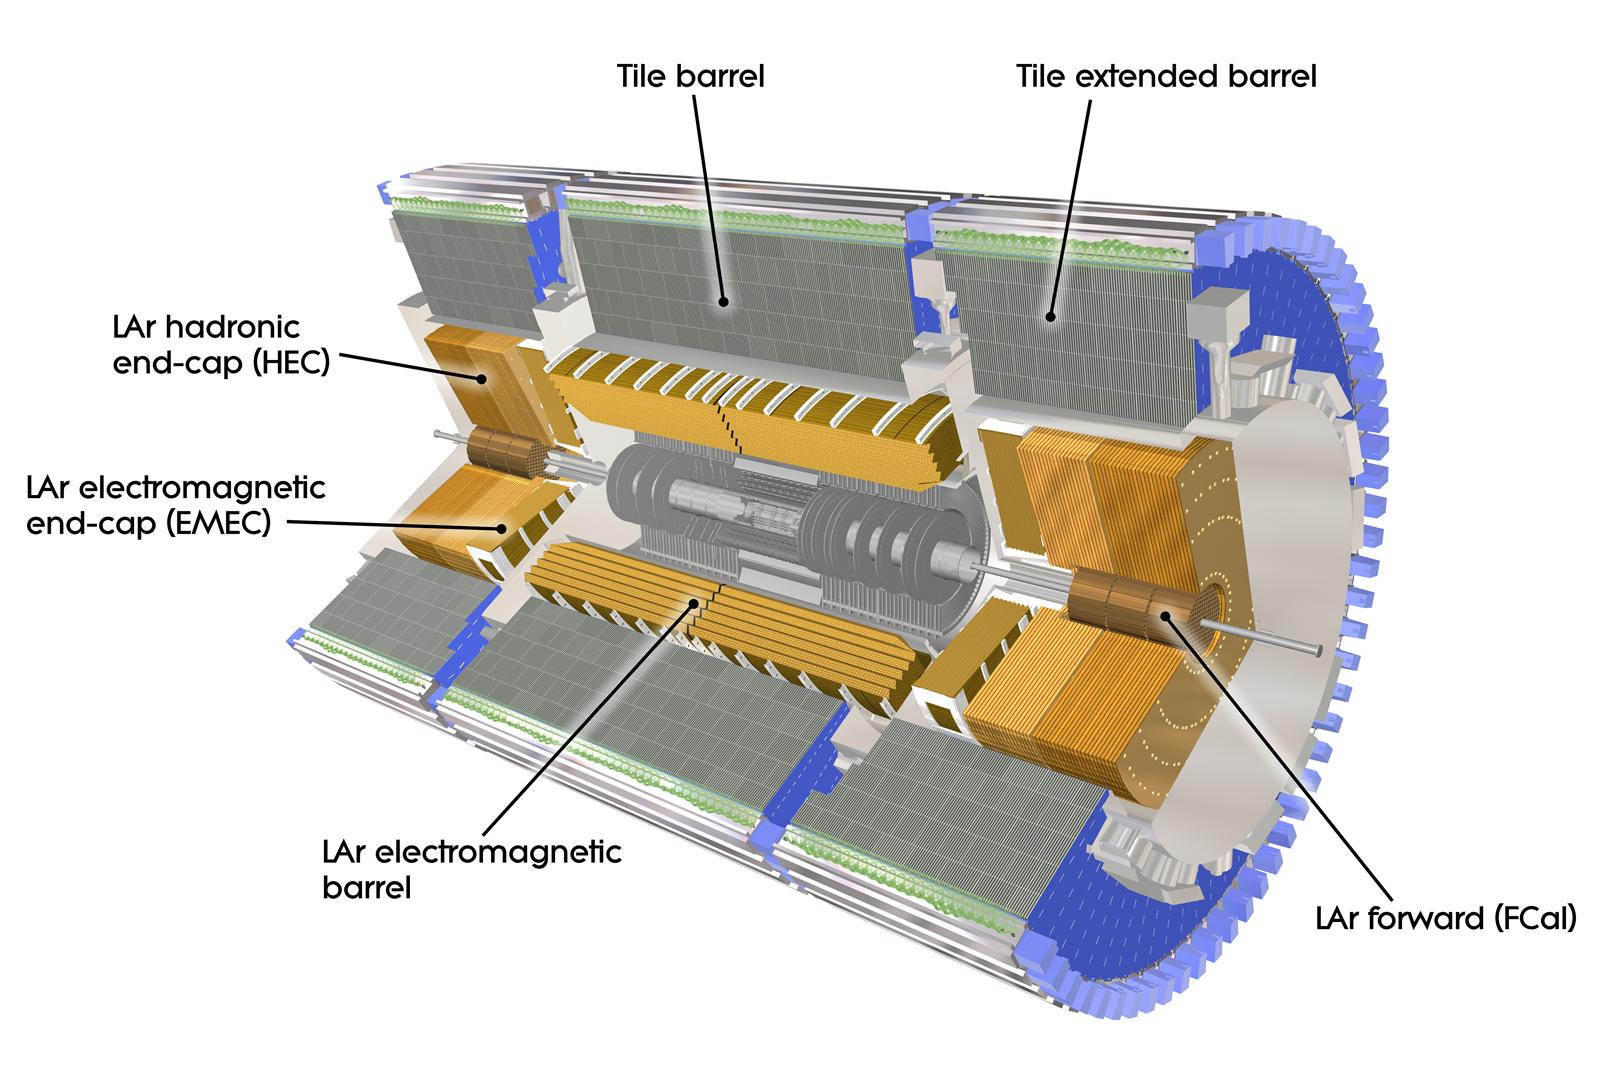
\includegraphics[width=0.95\textwidth]{figures/experiment/calorimetry_full.jpg}
    \caption{The ATLAS calorimeter system with its various components. Figure reproduced from Ref.~\cite{ATLAS2008}.}
    \label{fig:calorimetry-full}
\end{figure}

The ATLAS calorimeter system surrounds both the ID and the solenoid. It has a length of \SI{12.2}{\meter} and extends to an outer radius of \SI{4.25}{\meter}. Its geometry is fully symmetric in \(\varphi\) and has full coverage around the beam axis and covers the pseudorapidity range \(\abs{\eta} < 4.9\). The enormous energy of particles created in LHC \HepProcess{\Pp\Pp} collisions necessitates shortening of the absorption length by the use of calorimeters with alternating layers of active detector material and passive, purely absorbing material. This sampling calorimeter design is used in all ATLAS calorimeters.
The calorimeter system is comprised of electromagnetic calorimeters in the barrel and end-cap regions, enclosed by the hadronic calorimeters and complemented by dedicated calorimeters in the forward region close to the beam pipe. The ATLAS calorimeter system is hosted in three cryostats. The barrel cryostat contains the central solenoid and the electromagnetic barrel calorimeter. The end-cap cryostats each contain one electromagnetic end-cap calorimeter, one hadronic end-cap calorimeter, and one forward calorimeter.
The design of the calorimetry system ensures full containment of electromagnetic and hadronic showers and reduction of punch-through into the muon spectrometer. The electromagnetic calorimeters have more than \num{22} radiation lengths \(X_0\) in the barrel region and more than \num{24} radiation lengths in the end-cap regions. The hadronic calorimeters have an interaction length \(\lambda\) of approximately \num{9.8} in the barrel region and an interaction length of about \num{10} in the end-cap region. The forward calorimeter has an interaction length \(\lambda\) of approximately \num{10}.

The electromagnetic calorimeters cover the pseudorapidity range \(\abs{\eta} < 3.2\). The active detector medium is radiation hard Liquid Argon (LAr), which is chosen for its stability and linear response. The passive layers are made of lead. The absorber plates are shaped in an accordion geometry, thus providing full coverage in \(\varphi\) without cracks.
The barrel electromagnetic calorimeter covers the pseudorapidity range \(0 < \abs{\eta} < 1.475\). It consists of two identical components separated by a \SI{4}{\milli\meter} gap at \(\eta = 0\).
The two end-cap electromagnetic calorimeters (EMEC) cover the pseudorapidity range \(1.375 < \abs{\eta} < 3.2\). They consist each of two coaxial wheels with a small non-overlapping region at \(\abs{\eta} = 2.5\).
The transition region between the barrel and the end-cap (\(1.37 < \abs{\eta} < 1.52\)) contains a relatively large amount of inactive material.
In the precision physics region \(\abs{\eta} < 2.47\), where tracking information is available, the electromagnetic calorimeters are segmented in three layers with different granularity to allow for measurements of the electromagnetic shower profile.
The first layer is finely segmented in strips to allow for excellent discrimination between photons from the hard interaction and photons from \Pgpz decays. Most of the electron and photon energy is collected in the second layer, while the third layer measures the energy deposits due to the shower's tails.
The remaining acceptance is segmented in two layers with uniform granularity \(\Delta \phi \times \Delta \eta = 0.1 \times 0.1\).
The energy measurement in the region \(\abs{\eta} < 1.8\) is corrected for the energy loss of particles before entering the calorimeter by the use of two pre-sampling detectors, made of a thin LAr layer.
The combined electromagnetic calorimeter energy resolution is
\begin{align}
    \frac{\sigma_{E}}{E} = \frac{\SI{10}{\percent}}{\sqrt{E}} \oplus \SI{0.7}{\percent},
    \label{eq:experiment:ATLAS:calorimetry:resolution}
\end{align}
where \(\oplus\) indicates the quadratic sum.

The hadronic calorimeter encloses the electromagnetic calorimeters, as the depth of hadronic showers typically exceeds that of electromagnetic showers. Two different calorimeter technologies are employed to address the increasing irradiation in regions closer to the beam pipe.
The pseudorapidity range \(\abs{\eta} < 1.7\) is instrumented with a tile calorimeter, subdivided in a barrel region enclosing the electromagnetic barrel calorimeter and two extended barrel regions, which surround the end-cap calorimeters.
The barrel region covers \(\abs{\eta} < 1.0\) and the two extended barrel regions cover \(0.8 < \abs{\eta} < 1.7\).
Scintillator tiles are used as the active detector medium, while steel is used as the absorber medium.
The tile calorimeter extends \SIrange{2.28}{4.25}{\meter} in the radial direction. Each barrel region is azimuthally divided into 64 modules, corresponding to \(\Delta \varphi = 0.1\), and is segmented into three layers.
The scintillating tiles are read out by wavelength shifting fibres, which are grouped into photomultiplier tubes.
The tile calorimeter provides measurements with an energy resolution of \(\frac{\sigma_{E}}{E} = \frac{50\%}{\sqrt{E}}\).
The pseudorapidity range \(1.5 < \abs{\eta} < 3.2\)%
\footnote{The HEC is overlapping with both the tile calorimeter and the FCal to reduce drops in material density in the transition regions between the calorimeters.} %
is instrumented with a LAr hadron end-cap calorimeter (HEC). It consists of two cylindrical wheels per end-cap, both extending \SI{2.03}{\meter} in the radial direction and hosting each 32 identical wedge-shaped modules. Each wheel is longitudinally divided into two regions of depth and composed from copper plates interspersed with \SI{8.5}{\milli\meter} LAr gaps.
The combined hadronic calorimeter energy resolution for hadronic jets for tile and end-cap calorimeters is
\begin{align}
    \frac{\sigma_{E}}{E} = \frac{\SI{50}{\percent}}{\sqrt{E}} \oplus \SI{3}{\percent}.
\end{align}
The forward region is instrumented with a LAr forward calorimeter (FCal). It covers the pseudorapidity range \(3.1 < \abs{\eta} < 4.9\), thereby ensuring an almost hermetic coverage of the calorimetry system around the interaction point, which is essential for dark matter searches. The FCal consists of three modules in each end-cap, with the first made of copper targeting electromagnetic showers and the remaining two made of tungsten targeting hadronic interactions.
The forward region hadronic calorimeter has an energy resolution for hadronic jets of
\begin{align}
    \frac{\sigma_{E}}{E} = \frac{\SI{100}{\percent}}{\sqrt{E}} \oplus \SI{10}{\percent}.
\end{align}


\subsection{Muon Spectrometer}
\label{sec:experiment:ATLAS:muons}
As muons are substantially heavier than electrons, they do not lose energy by bremsstrahlung and leave only a track footprint because of ionisation energy loss in the calorimeter. Consequently, the particles emerging from the calorimeters are considered to be muons and are detected by a dedicated detector system. The muon spectrometer provides measurements of charged particles exiting the calorimeters, covering the pseudorapidity range \(\abs{\eta} < 2.7\).
It is also able to provide track information in coarser granularity but with timing resolution within a few tens of a nanosecond for the sake of triggering or bunch crossing identification in the pseudorapidity range \(\abs{\eta} < 2.4\). To this end, the muon spectrometer is equipped with sets of precision tracking detectors and trigger chambers. The magnetic field provided by the toroid magnets allows measuring the muon momentum based on the sagitta of the curved trajectory. The detector resolution is optimised for measurements in the plane in the principal bending direction, the so-called bending plane. The layout of the ATLAS muon spectrometer is shown in \Cref{fig:muonspectrometer-full}.

\begin{figure}[htbp]
    \centering
    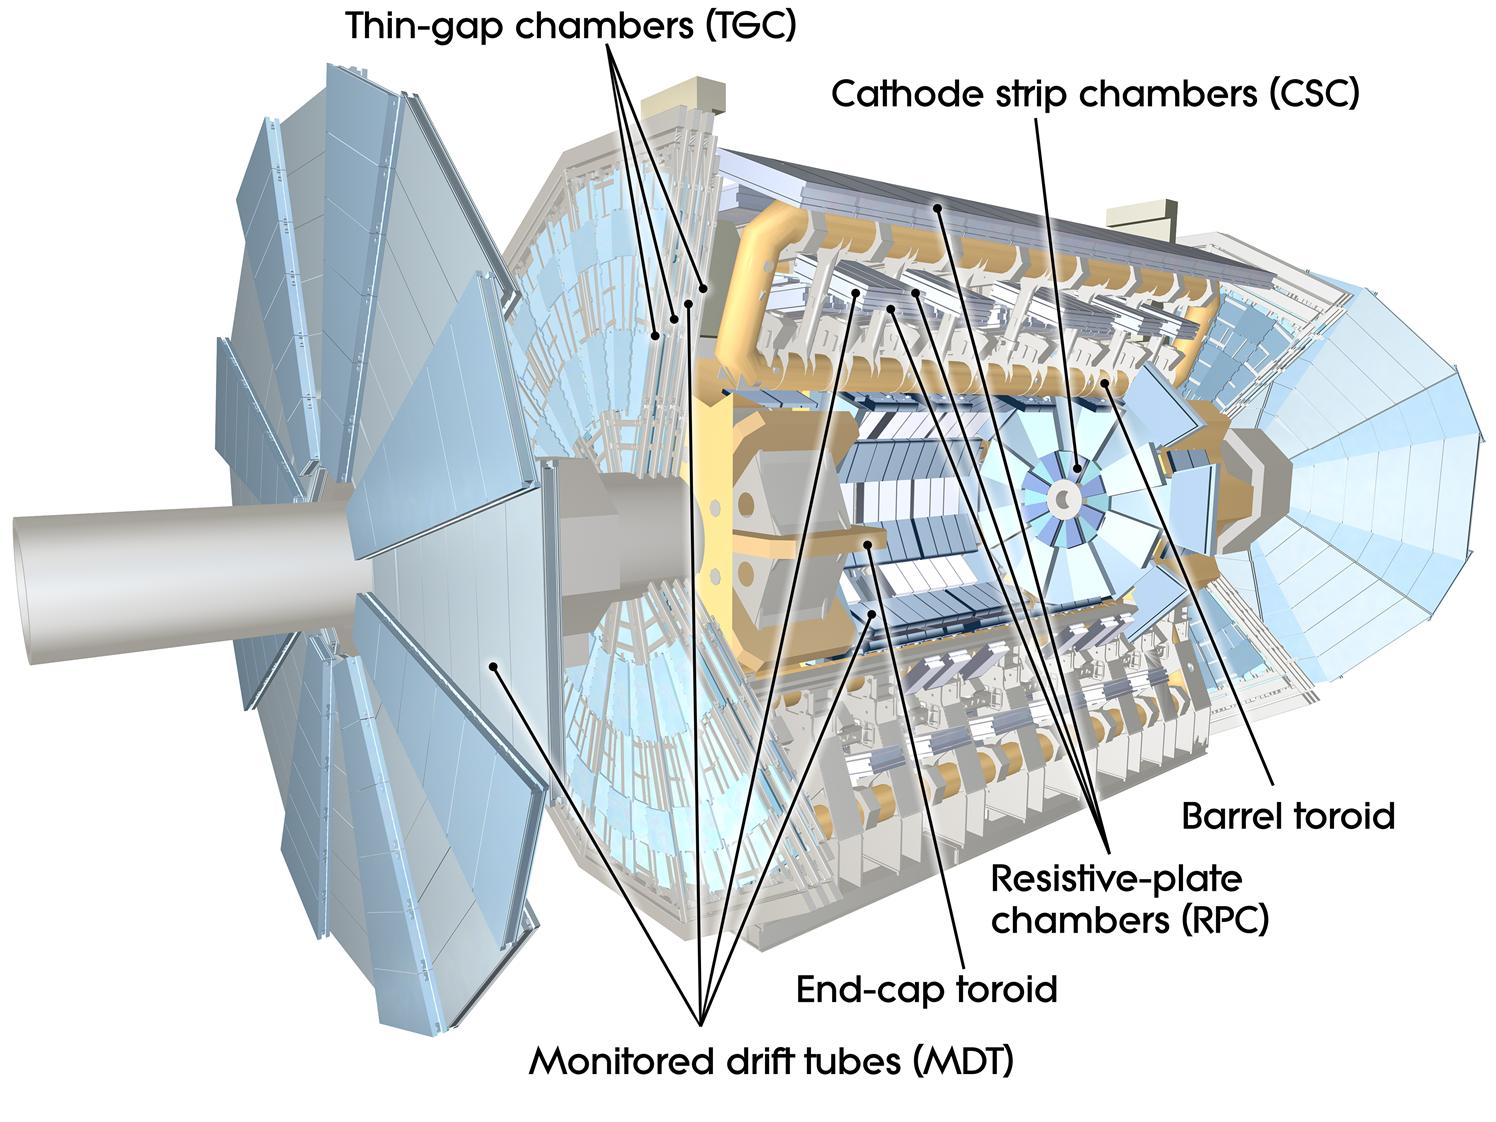
\includegraphics[width=0.95\textwidth]{figures/experiment/muonspectrometer_full.jpg}
    \caption{The ATLAS muon spectrometer with its various components. Figure reproduced from Ref.~\cite{ATLAS2008}.}
    \label{fig:muonspectrometer-full}
\end{figure}

The \num{1150} monitored drift tube (MDT) chambers, whose length and shape depends on their position in the detector, perform the precision measurements.
In the barrel region, they are located between and on the toroid coils. The symmetry of the toroid magnet is reflected in the muon system's geometry, which is divided into octants.
Each octant is subdivided in the azimuthal direction into a large and small sector. The overlap between the different sector types minimises gaps in acceptance and allows for relative alignment of adjacent sectors using tracks measured in both sectors. The chambers in the barrel region are arranged in three concentric cylindrical shells, located at \SI{5}{\meter}, \SI{7.5}{\meter}, and \SI{10}{\meter} in the radial distance to the beam axis.
In the end-cap region the MDT chambers form four large wheels perpendicular to the \(z\)-axis, which are located in front and behind the end-cap toroid magnet. They are located at distances of \(\abs{z}=\SI{7.4}{\meter}\), \(\abs{z}=\SI{10.8}{\meter}\), \(\abs{z}=\SI{14}{\meter}\), and \(\abs{z}=\SI{21.5}{\meter}\) to the interaction point.
An MDT chamber consists of two multi-layers with three or four layers of drift tubes per multi-layer, operated at an absolute pressure of \SI{3}{\bar}. The drift tubes are made of aluminium with a tungsten-rhenium anode wire in the centre. The detection principle is similar to the TRT operation, described in \Cref{sec:ATLAS-ID}. The resolution of a single drift tube on average is \SI{35}{\micro\meter}.
MDT chambers provide position measurements in the bending plane with \SI{35}{\milli\meter} resolution.
The sagitta-based measurement achieves an excellent momentum resolution, based on both precise measurements of muon trajectories and precise knowledge of the chamber positions within \SI{30}{\micro\meter}. To this end, each chamber is equipped with a RASNIK optical alignment system, which monitors mechanical deformations of the chambers and movements of the chambers relative to each other.

In the pseudorapidity range \(2 < \abs{\eta} < 2.7\), the innermost wheel is instrumented with \num{32} cathode strip chambers (CSC) instead of MDT chambers, in order to meet the demands on rate capability and time resolution. The CSC chambers are multi-wire proportional chambers with cathode plates segmented into strips in orthogonal directions, enabling measurements of two coordinates from the charge-induced signal distribution. They provide position measurements with \SI{40}{\micro\meter} in the bending plane and \SI{5}{\milli\meter} in the transverse plane.

The precision tracking detectors are complemented by a system of fast trigger chambers. In the barrel region, extending up to \(\abs{\eta} < 1.05\), \num{606} resistive plate chambers (RPC) are employed for providing fast detection of muons with a timing of \SI{1.5}{\nano\second}. The RPC chambers provide measurements with a resolution of \SI{10}{\milli\meter} in both the bending plane and the azimuthal plane.
The end-cap region, covering the pseudorapidity range from \(1.05 < \abs{\eta} < 2.4\), is instrumented with thin gap chambers (TGC) with timing of \SI{4}{\nano\second}. They provide measurements with a resolution of \SIrange{2}{6}{\milli\meter} in the bending plane and \SIrange{3}{7}{\milli\meter} in the azimuthal plane.

\subsection{Trigger}
\label{sec:experiment:ATLAS:trigger}
The event rate of \HepProcess{\Pp\Pp} interactions at the design luminosity \SI{e34}{\per\centi\meter\per\second} is \(\mathcal{O}(\SI{1}{\giga\hertz})\). Using a popular analogy, sampling physics from the LHC is like drinking water from a fire hose~\cite{Campbell2018}. As technical constraints limit the maximum possible event recording rate to \SI{1}{\kilo\hertz}, a highly selective trigger system is required to filter events associated with processes of interest. The ATLAS Trigger and Data Acquisition (TDAQ) systems consist of a hardware-based Level-1 (L1) trigger, followed by a software-based high-level trigger (HLT). The schematics of the TDAQ system are shown in \Cref{fig:trigger-scheme}.

\begin{figure}[htbp]
    \centering
    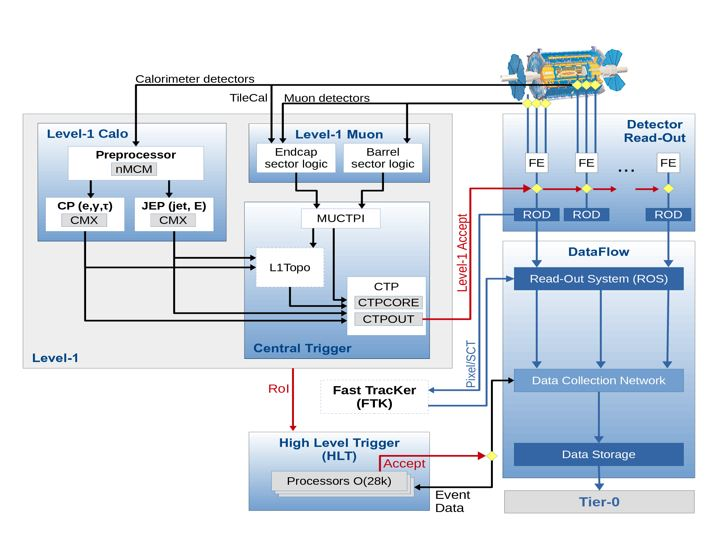
\includegraphics[width=0.95\textwidth]{figures/experiment/trigger.jpg}
    \caption{The ATLAS trigger logic in Run-2. Figure reproduced from Ref.~\cite{Ruiz-Martinez:2133909}.}
    \label{fig:trigger-scheme}
\end{figure}

The L1 trigger system reduces the data rate to approximately \SI{100}{\kilo\hertz}. It uses a subset of the full detector information to decide between keeping or discarding events within a latency of \SI{2.5}{\micro\second}. The L1 trigger decision is formed in the Central Trigger Processor (CTP), which receives information from the L1 calorimeter (L1 Calo) and the L1 muon (L1 Muon) triggers.

The L1 Calo trigger processes analogue signals from the electromagnetic and hadronic calorimeters, which are digitised and calibrated by a preprocessor system in approximately 7000 trigger towers with a granularity of \(\Delta \eta \times \Delta \phi = 0.1 \times 0.1\).
Electron, photon and hadronically decaying \(\tau\) lepton candidates with specified energy thresholds and isolation criteria\footnote{Isolation implies that the energetic particle must have a minimum angular separation from any other significant energy deposit in the same event.} are identified by the Cluster Processor (CP). A Jet/Energy-sum Processor (JEP) is able to reconstruct jet candidates and compute scalar and missing energy sums from trigger elements with \(\Delta \eta \times \Delta \phi = 0.2 \times 0.2\) granularity.
The L1 Muon trigger processes signals from three stations.

The L1 Muon trigger processes signals from either three stations of RPC chambers in the barrel region or from three stations of TGC chambers in the end-cap. The principle underpinning the muon trigger is a coincidence of hits in the different trigger stations within the road of a muon candidate. The hit in the trigger chamber layer, which is referred to as the pivot plane, defines the infinite momentum track as the connecting line to the interaction point. As the muon candidate's \(p_{\text{T}}\) affects the curvature and consequently the width of the muon road, the deviation of a hit in other chamber layers from the infinite momentum track is used for a quick momentum estimate through a programmable coincidence logic. Three low-\(p_{\text{T}}\) thresholds (\SI{4}{\giga\electronvolt}, \SI{6}{\giga\electronvolt}, and \SI{10}{\giga\electronvolt}) are defined by coincidence windows using information from two trigger chamber layers. In addition, three high-\(p_{\text{T}}\) thresholds (\SI{11}{\giga\electronvolt}, \SI{15}{\giga\electronvolt}, and \SI{20}{\giga\electronvolt}) are defined by taking into account additional coincidence requirements with regard to the third layer.
The trigger signals from the barrel and end-cap triggers are combined into a set of six threshold multiplicities for each bunch crossing in the muon to CTP interface and passed on to the CTP.

Events accepted by the L1 trigger are buffered in the Read-Out System (ROS), awaiting further confirmation from the HLT.
The HLT decision is evaluated by a computing farm, which can run reconstruction algorithms with the same precision used in the offline reconstruction, with access to the event information in full granularity. It receives Region-of-Interest (RoI) information, consisting of essential features identified by the L1 trigger and the geographical coordinates of those regions within the detector where its selection process has identified those features. These form a starting point for the HLT algorithms. Their significantly better particle identification and momentum resolution sharpens the HLT decision and thus reduces the final data-taking rate to approximately \SI{200}{\hertz}.

\subsection{Grid computing}
\label{sec:experiment:ATLAS:computing}
Large-scale computing infrastructure is required to analyse a large amount of data recorded by the LHC experiments.
The Worldwide LHC Computing Grid (WLCG) is designed to preserve, distribute and analyse LHC collision data. It is a distributed computing grid, consisting of more than \num{160} computing centres in more than 40 countries. Different tiers hierarchically structure the role of  computing centres:
\begin{itemize}
    \item The Tier-0 centre is located at the CERN data centre and is responsible for the first-pass reconstruction.
    \item The thirteen Tier-1 centres receive raw data and reconstruction output from Tier-0 and are responsible for the safe-keeping of a proportional share of data and simulations and large-scale reprocessing.
    \item The over 160 Tier-2 centres are typically hosted by universities and other scientific institutes. They provide storage and adequate computing power for specific analysis tasks.
    \item Tier-3 resources refer to computing clusters offered by research institutions to individual users. There is no formal engagement between WLCG and Tier 3 resources, but they often provide access to the respective WLCG sites.
\end{itemize}


% % !TEX root = ../my-thesis.tex
%
\chapter{Experimental methods}
\label{ch:methods}

\cleanchapterquote{The idea of a method that contains firm, unchanging, and absolutely binding principles for conducting the business of science meets considerable difficulty when confronted with the results of historical research.}{Paul Feyerabend}{Against Method. London: New Left Books, 1975}

The experimental methods for analysing the recorded data set of \HepProcess{\Pp\Pp} collision events are outlined in this Chapter. \Cref{sec:methods:event-reconstruction} describes the algorithms used for the reconstruction of compound physics objects. The statistical techniques used to obtain results from fits of the statistical model to data are described in \Cref{sec:methods:statistics}. The RECAST framework, which enables faithful and efficient reinterpretation of searches, is introduced in \Cref{sec:methods:recast}.

\section{Event reconstruction}
\label{sec:methods:event-reconstruction}
\subsection{Introduction}
\label{sec:methods:event-reconstruction:intro}
The various sub-systems of the ATLAS detector record detailed information about the \HepProcess{\Pp\Pp} collisions, which occur in the interaction region. The elementary detector signatures are the hits in the sensitive tracking detector planes and the energy deposits in the calorimeters. These measurements serve as inputs for sophisticated reconstruction algorithms, which define compound physical objects, such as electrons, photons, muons, tau leptons, jets, and missing transverse momentum. These compound physical objects are used to define the selection requirements in the searches for dark matter and to construct discriminating observables for the statistical analysis.

The object reconstruction is subject to inefficiencies in the particle identification and afflicted with systematic uncertainties due to various detector effects. The reconstructed kinematic properties of the compound physical objects can deviate from their true value for the same reasons. These discrepancies can be reduced to some extent by employing calibration methods. In the ATLAS collaboration, the standard recommendations for object identification, reconstruction, calibration, and evaluation of the associated systematic uncertainties are centrally provided by the Combined Performance (CP) groups.


\subsection{Reconstruction of basic objects}
\label{sec:methods:event-reconstruction:basic}
All reconstructed physics objects are based on reconstructed tracks, vertices, and topological clusters.

\textbf{Tracks} are reconstructed by connecting the hits in different layers of the ID. Their momentum and charge can be inferred from their deflection in the solenoidal magnetic field.
The tracks are parametrised, as shown in \Cref{fig:methods:event-reconstruction:tracks:parametrisation}, by a set of five parameters
\begin{itemize}
	\item the transverse and longitudinal impact parameters \(d_{0}\) and \(z_{0}\),
	\item the azimuthal and polar angles \(\varphi\) and \(\theta\), and
	\item the ratio of charge and transverse momentum \(q / \pt\).
\end{itemize}
Tracks are reconstructed by a set of tracking algorithms~\cite{ATLAS-CONF-2012-042,PERF-2015-08}.
Two approaches --- an ``inside-out'' algorithm, mostly sensitive to primary charged particles produced in the \HepProcess{\Pp\Pp} interaction, and an ``outside-in'' algorithm, mostly sensitive to secondary decay products --- are employed to ensure high reconstruction efficiency. The ``inside-out'' algorithm considers seeds containing three hits in the silicon PXD and SCT detectors and extends the track seed to the TRT using a combinatorial Kalman filter~\cite{Frhwirth1987} to add hits further away from the interaction point. The ``outside-in'' algorithm considers TRT track segments and extrapolates them to the vicinity of the interaction point by adding hits in the silicon detectors, which have not been associated with tracks yet. All ID tracks are required to satisfy \(\pt > \SI{0.4}{\giga\electronvolt}\) and \(\abs{\eta} < 2.4\). The impact parameter resolution is shown in \Cref{fig:methods:event-reconstruction:tracks:impactparameter-resolution}.
In addition to the tracks in the ID, the muon reconstruction employs tracks recorded by the MS. These are reconstructed by dedicated algorithms based on Hough transforms or iterative combination of hits~\cite{Nicolaidou2008}.

\begin{figure}[htbp]
	\centering
	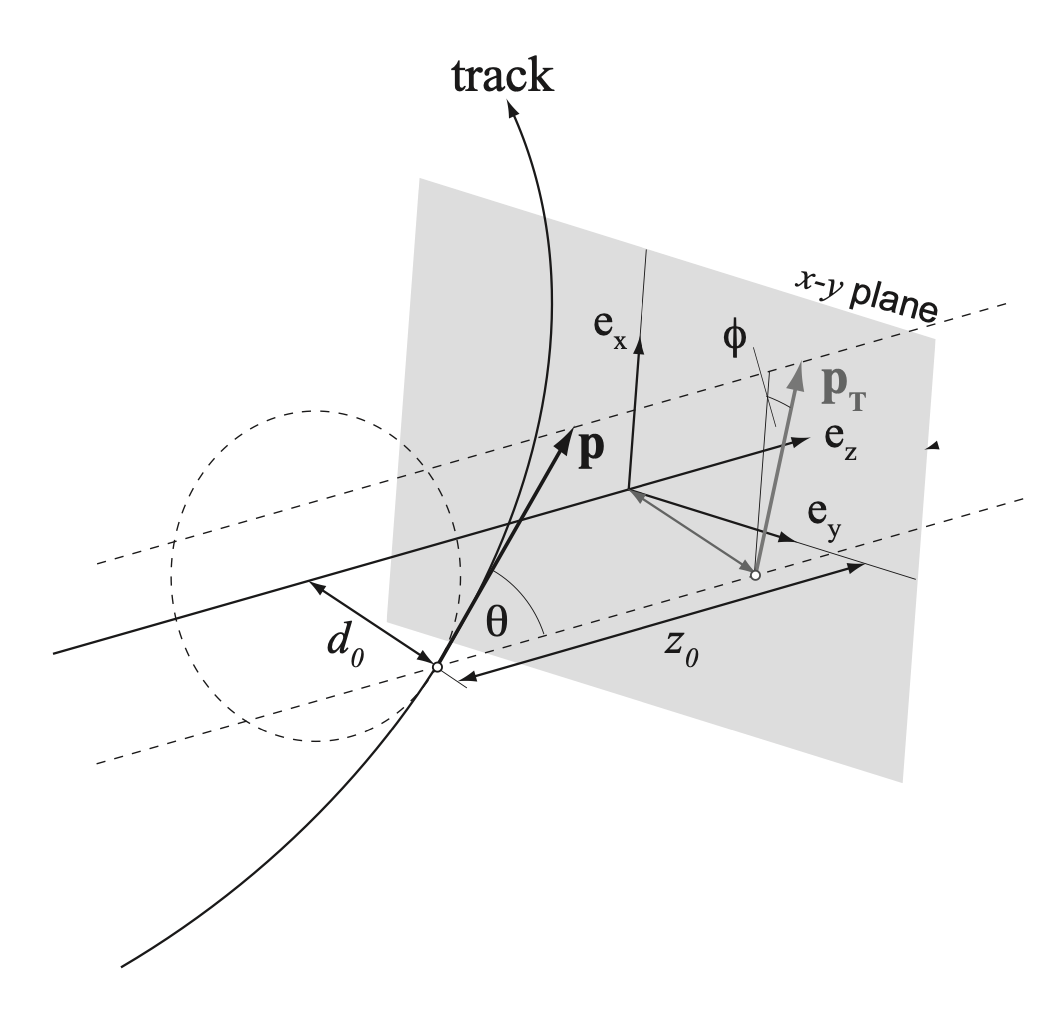
\includegraphics[width=0.73\textwidth]{figures/methods/track.png}
	\caption{A track parametrised with respect to the nominal \(z\)-axis through the azimuthal angle \(\varphi\), the polar angle \(\theta\), the charged inverse momentum \(q / p\), and the transverse and longitudinal impact parameters \(d_{0}\) and \(z_{0}\). Figure reproduced from Ref.~\cite{Cornelissen2007}.}
	\label{fig:methods:event-reconstruction:tracks:parametrisation}
\end{figure}

\begin{figure}[htbp]
	\centering
	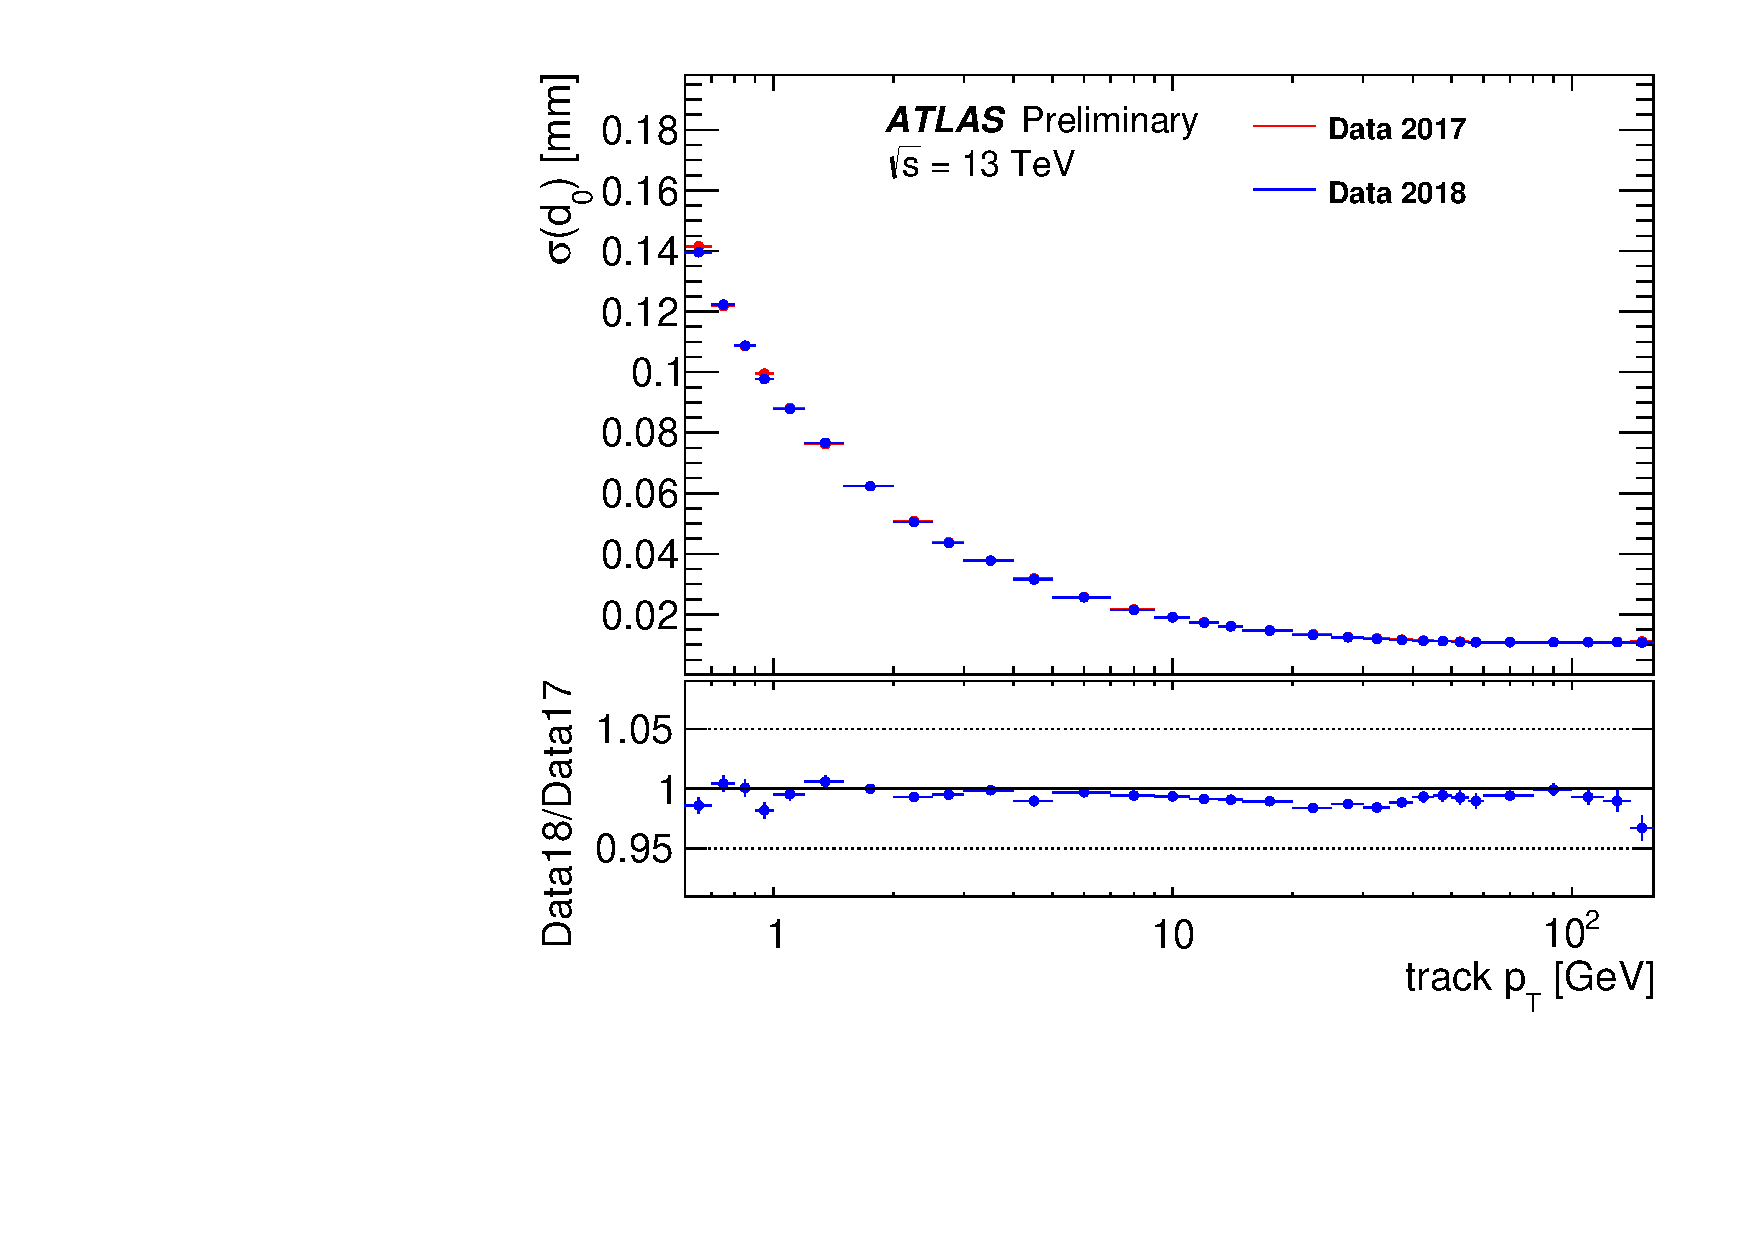
\includegraphics[width=0.45\textwidth]{figures/methods/tracking_resolution_d0.pdf}
	\hfill
	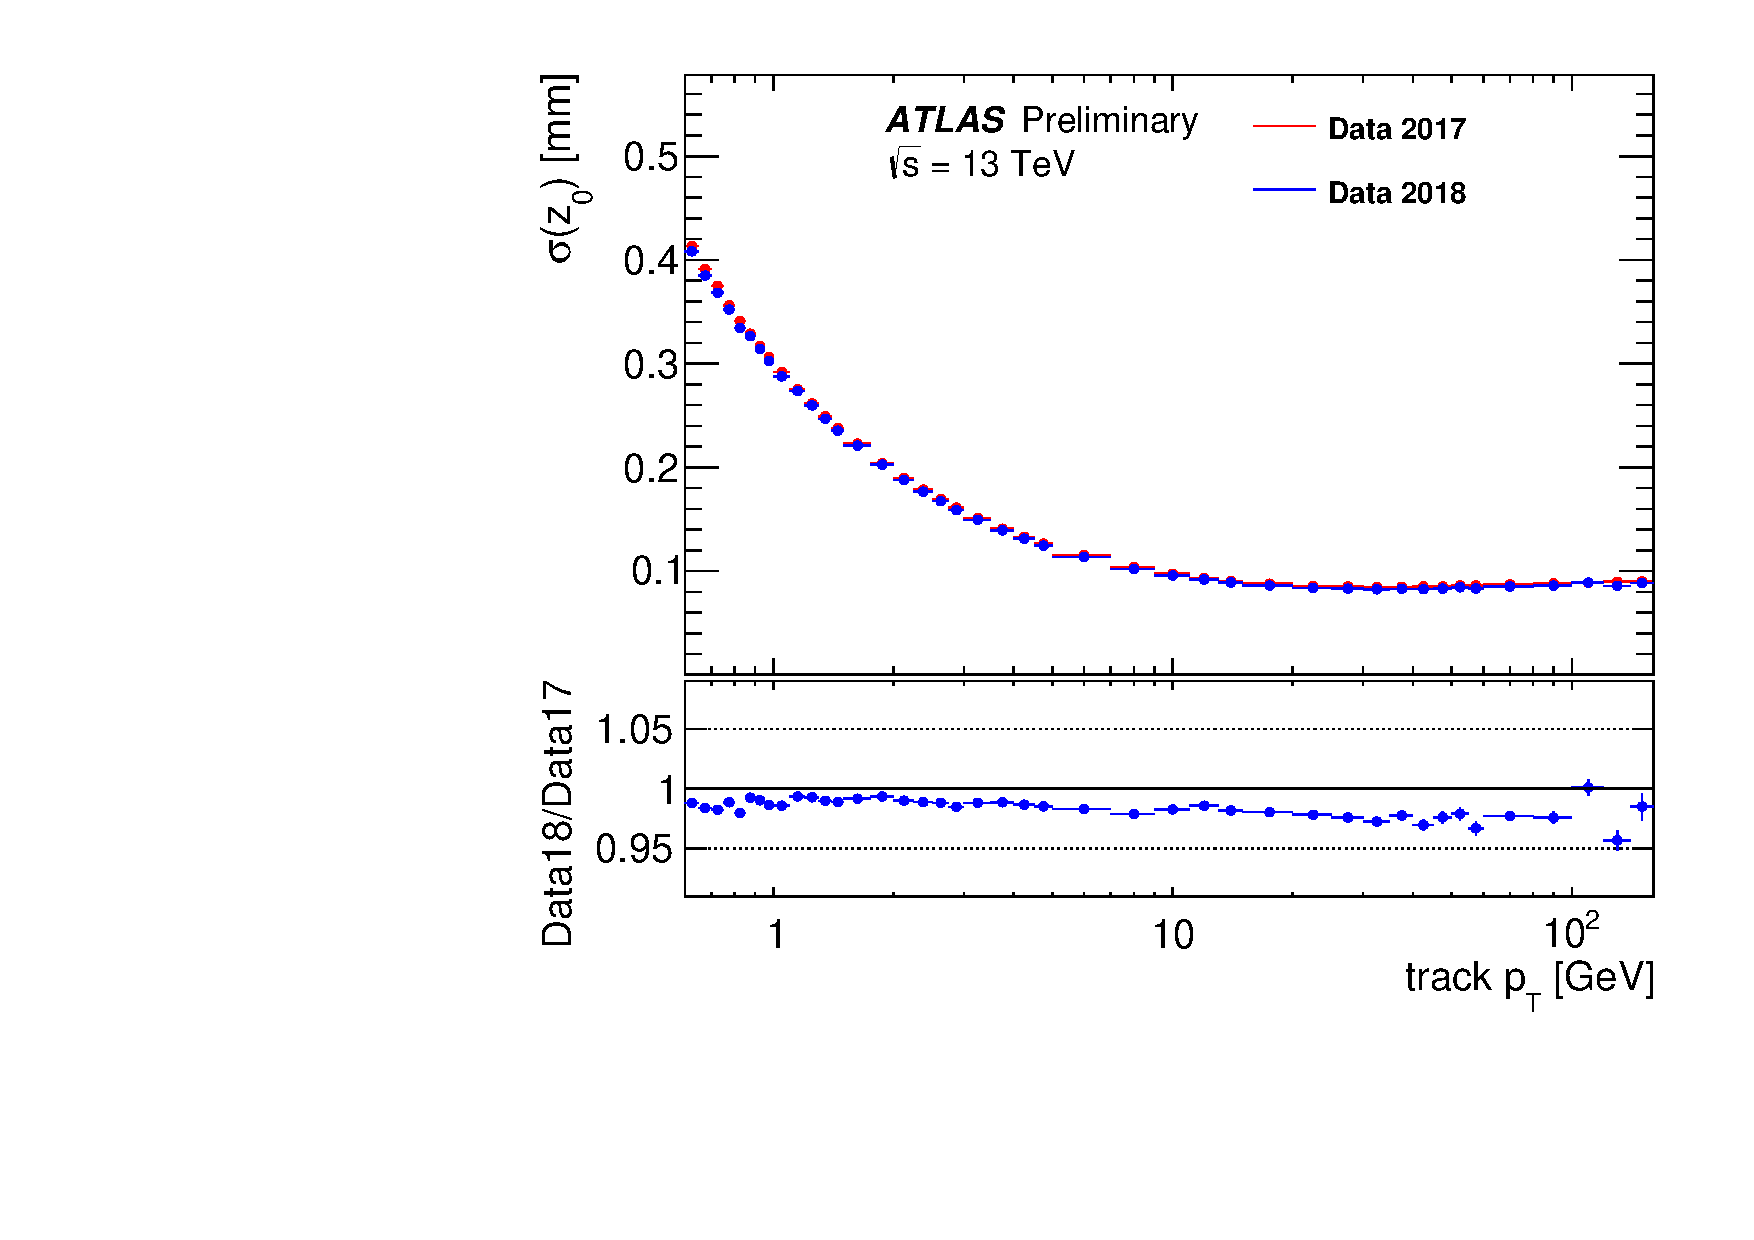
\includegraphics[width=0.45\textwidth]{figures/methods/tracking_resolution_z0.pdf}
	\caption{Resolution of the transverse impact parameter \(d_{0}\) and the longitudinal impact parameter \(z_{0}\) of tracks associated with jets with \(\pt > \SI{20}{\giga\electronvolt}\), measured in \HepProcess{\Pp\Pp} collision data recorded in 2017 and 2018 with dijet triggers. Figure reproduced from Ref.~\cite{IDTR-2018-008}.}
	\label{fig:methods:event-reconstruction:tracks:impactparameter-resolution}
\end{figure}

\textbf{Vertices} are defined as points at which either a \HepProcess{\Pp\Pp} interaction or a decay takes place. The iterative reconstruction of vertices employs tracks and consists of two steps~\cite{Boutle2017}.
\begin{enumerate}
	\item Vertex finding. The vertices in a collision event are reconstructed using tracks satisfying certain quality criteria, including \(\abs{d_{0}} < \SI{4}{\milli\meter}\) and requirements on the impact parameter resolution \(\sigma(d_{0}) < \SI{5}{\milli\meter}\) and \(\sigma(z_{0}) < \SI{10}{\milli\meter}\). The seed position for the first vertex is defined by the transverse coordinates of the beam spot and the \(z\)-coordinates or tracks at their points of closest approach to the beam spot.
	All vertices require at least two associated tracks.
	\item Vertex fitting. The tracks and the seed are used to estimate the best vertex position with a fit based on an iterative annealing procedure. In each iteration of the fit, the weights of less compatible tracks are decreased, to determine the best vertex position.
\end{enumerate}
The primary vertex (PV) is the point at which a hard scattering process in the \HepProcess{\Pp\Pp} interaction occurred. It is reconstructed as the vertex with the largest sum of squared transverse momenta of all tracks associated with it. \Cref{fig:methods:event-reconstruction:vertex:performance} shows the vertex performance in two runs of 2018 \HepProcess{\Pp\Pp} data with different average number of interactions per bunch crossing.

\begin{figure}[htbp]
	\centering
	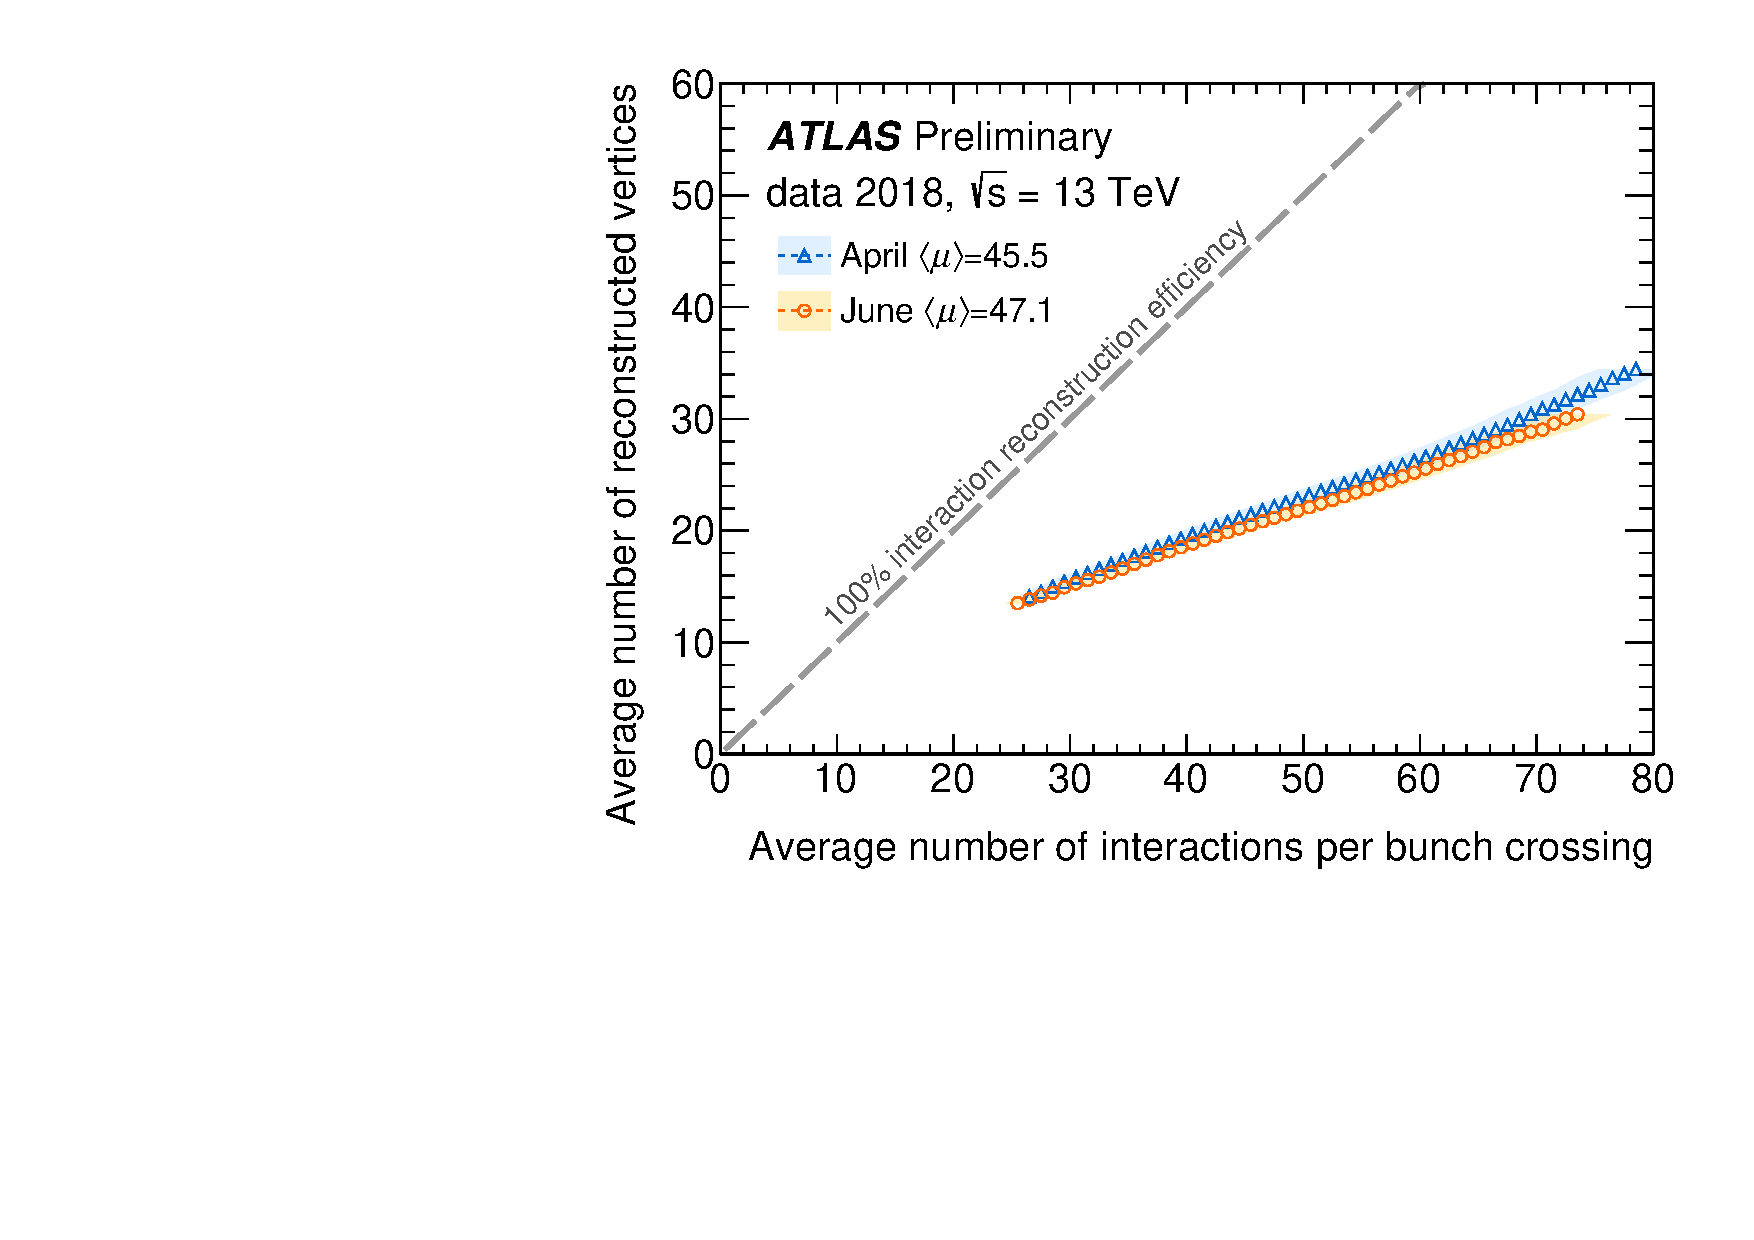
\includegraphics[width=0.75\textwidth]{figures/methods/vertex_efficiency.pdf}
	\caption{Vertex performance in 2018 \HepProcess{\Pp\Pp} data, indicated by the number of reconstructed vertices in dependence of the average number of interactions per bunch crossing. Figure reproduced from Ref.~\cite{IDTR-2018-008}.}
	\label{fig:methods:event-reconstruction:vertex:performance}
\end{figure}


\textbf{Topological clusters} are groups of topologically connected energy deposits in neighbouring calorimeter cells due to incident particles. Their reconstruction~\cite{PERF-2014-07} is seeded by energy deposits which are significantly greater than the expected noise due to the detector electronics and pile-up events. The reconstruction is based on the cell signal significance \(\xi = E_{\text{cell}} / \sigma(E_{\text{cell}})\), which is defined as the ratio of the detector signal \(E_{\text{cell}}\) and the expected noise \(\sigma(E_{\text{cell}})\) on the electromagnetic scale. All calorimeter cells adjacent to the seed cells, which satisfy certain noise-suppression thresholds, are iteratively added to form ``proto-clusters''. These ``proto-clusters'' are subsequently split if they contain two or more local maximums of the detector signal with \(E_{\text{cell}} > \SI{500}{\mega\electronvolt}\) to separate individual showers.
The clusters are parametrised by the azimuthal and polar angles defined by the energy-weighted barycentre of the associated calorimeter cells and by the cluster energy.
The cluster energy can be calibrated to different scales to adequately describe the physical objects initiating the shower in the calorimeters~\cite{PERF-2014-02}.
\begin{itemize}
	\item Electromagnetic (EM) scale calibration. Topological clusters in their basic definition are reconstructed at the EM scale to describe particles depositing their energy in the calorimeter via electromagnetic showers.
	\item Local Calibration Weighting (LCW) calibration. This alternative calibration~\cite{PERF-2011-03} takes into account the response of the calorimeter to hadrons produced in the interaction point. Clusters are classified either as electromagnetic or hadronic before the appropriate energy corrections derived from single pion MC simulations are applied. The LCW calibration can improve the energy resolution of reconstructed jets in comparison to jets based on EM-scale clusters.
\end{itemize}

\subsection{Electrons}
\label{sec:methods:event-reconstruction:electrons}
Electrons passing the ATLAS detector leave a track in the ID and initiate an electromagnetic shower in the high-granularity EM calorimeter. The electron candidates are reconstructed based on the combined information of the two sub-detectors.
The performance of the electron reconstruction, identification, and isolation algorithms is evaluated in data and simulated MC samples using electrons from \HepProcess{\PZ \to \Pem \Pep} and \HepProcess{\PJgy \to \Pem \Pep} decays.

\subsubsection{Electron reconstruction}
Electron candidates are reconstructed by matching reconstructed tracks to clusters in the EM calorimeter. The coverage of the ID limits the electron reconstruction to \(\abs{\eta} < 2.47\). The path of an electron through the detector is shown in \Cref{fig:methods:event-reconstruction:electrons:path}.

\begin{figure}[htbp]
	\centering
	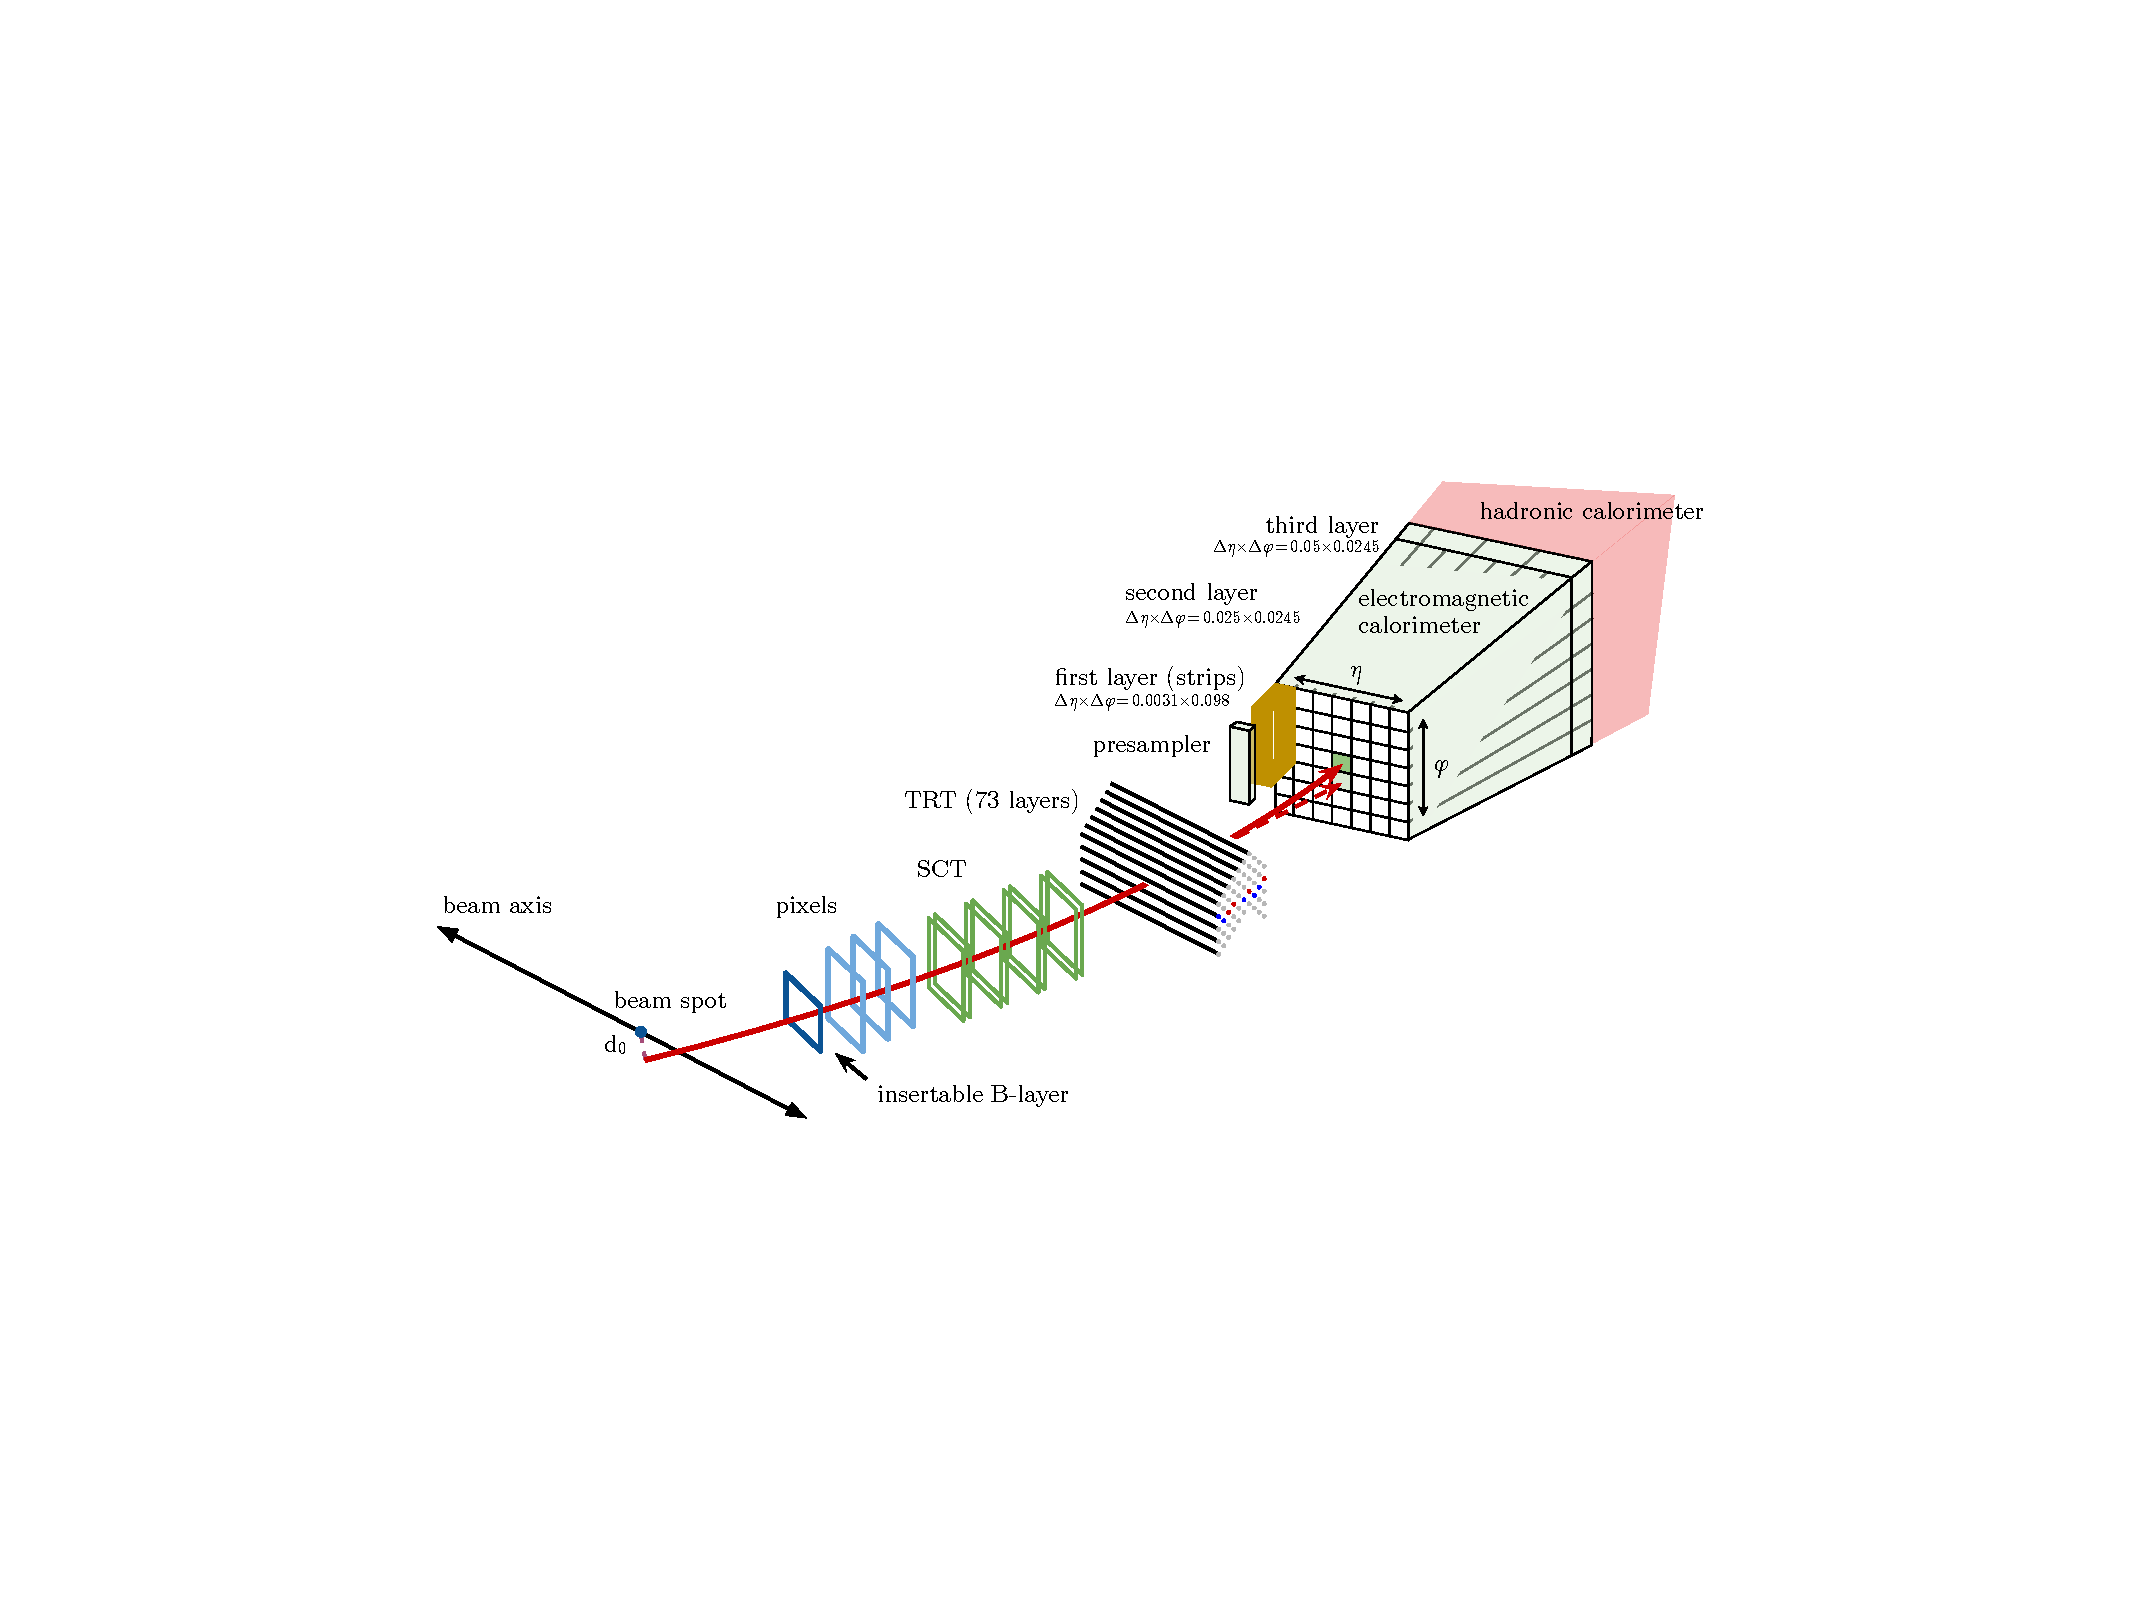
\includegraphics[width=0.95\textwidth]{figures/methods/electron.pdf}
	\caption{Schematic illustration of an electron's trajectory (red) through the detector, first traversing the tracking system comprised of PXD detectors, SCT detectors and lastly the TRT, and then enters the EM calorimeters. The dashed trajectory (red) illustrates the path of a photon radiated off the electron due to interactions with the detector material. Figure reproduced from Ref.~\cite{PERF-2017-01}.}
	\label{fig:methods:event-reconstruction:electrons:path}
\end{figure}

The electron reconstruction~\cite{PERF-2017-01} starts from fixed-size seed clusters, which are selected by a sliding-window algorithm. The inputs to the algorithms are towers of calorimeter cells in the first three calorimeter layers, which have a granularity of \(\Delta \eta \times \Delta \varphi = 0.025 \times 0.025\).
The algorithm considers seeds composed of \(N_{\eta} \times N_{\varphi} = 3 \times 5\) towers of EM calorimeter cells, which are required to have a minimal energy deposit of \(E_{\text{T}} > \SI{2.5}{\giga\electronvolt}\).

ID tracks are matched to the clusters using the distance measure \(\Delta R\) between the position of the track extrapolated to the middle layer of the calorimeter and the cluster barycentre. The tracks are re-fitted with the Gaussian Sum Filter (GSF)~\cite{ATLAS-CONF-2012-047} algorithm to account for Bremsstrahlung effects. The resulting electron candidate consists of a cluster seed, which is successfully matched to at least one track.

In the 2017--2018 data taking campaign, new electron reconstruction algorithms are employed~\cite{ATL-PHYS-PUB-2017-022,EGAM-2018-01}. These algorithms replace the electron reconstruction based on fixed-size windows with a dynamic approach based on variable-size topological clusters.

\subsubsection{Electron identification}
The electron identification (ID) algorithm discriminates between electron candidates from signal processes, such as prompt production in the hard-scattering vertex or from the decay of heavy resonances, and background-like objects, such as hadronic jets or converted photons. A likelihood-based approach (LH) is employed, which considers the information provided by clusters and tracks, such as the resolution parameters of the associated tracks and the calorimeter shower shape. The LH based discriminant and the number of hits in the track are used to calculate the probability of an electron candidate being either an electron from signal processes or a background-like object.

Three electron ID operating points (OPs) with increasing background rejection are defined.
The \textsc{Loose} OP corresponds to an average electron identification efficiency of \SI{93}{\percent}.
Similarly, the \textsc{Medium} and \textsc{Tight} OPs correspond to efficiencies of \SI{88}{\percent} and \SI{80}{\percent}, respectively.
These points are inclusive, meaning that the \textsc{Tight} electrons are a subset of the \textsc{Medium} electrons and the \textsc{Medium} electrons are a subset of the \textsc{Loose} electrons. In addition, the \textsc{LooseAndBLayer} OP is defined as a variation of the \textsc{Loose} OP with the additional requirement of at least one hit in the innermost layer of the PXD detector.
Out of these definitions, \textsc{Loose} and \textsc{LooseAndBLayer} electrons are considered in the searches for dark matter presented in this dissertation.

The electron identification efficiency in bins of \(E_{\text{T}}\) and \(\eta\) is shown in \Cref{fig:methods:event-reconstruction:electrons:identification}. The identification efficiency gradually increases from low to high \(E_{\text{T}}\). In the range \(\SI{20}{\giga\electronvolt} < E_{\text{T}} < \SI{50}{\giga\electronvolt}\), the \textsc{Medium} and \textsc{Tight} OPs have an improved rejection of background processes by \num{2.0} and \num{3.5}, respectively, with respect to the \textsc{Loose} OP.
\begin{figure}[htbp]
    \centering
    \begin{subfigure}{1.\textwidth}
      \centering
      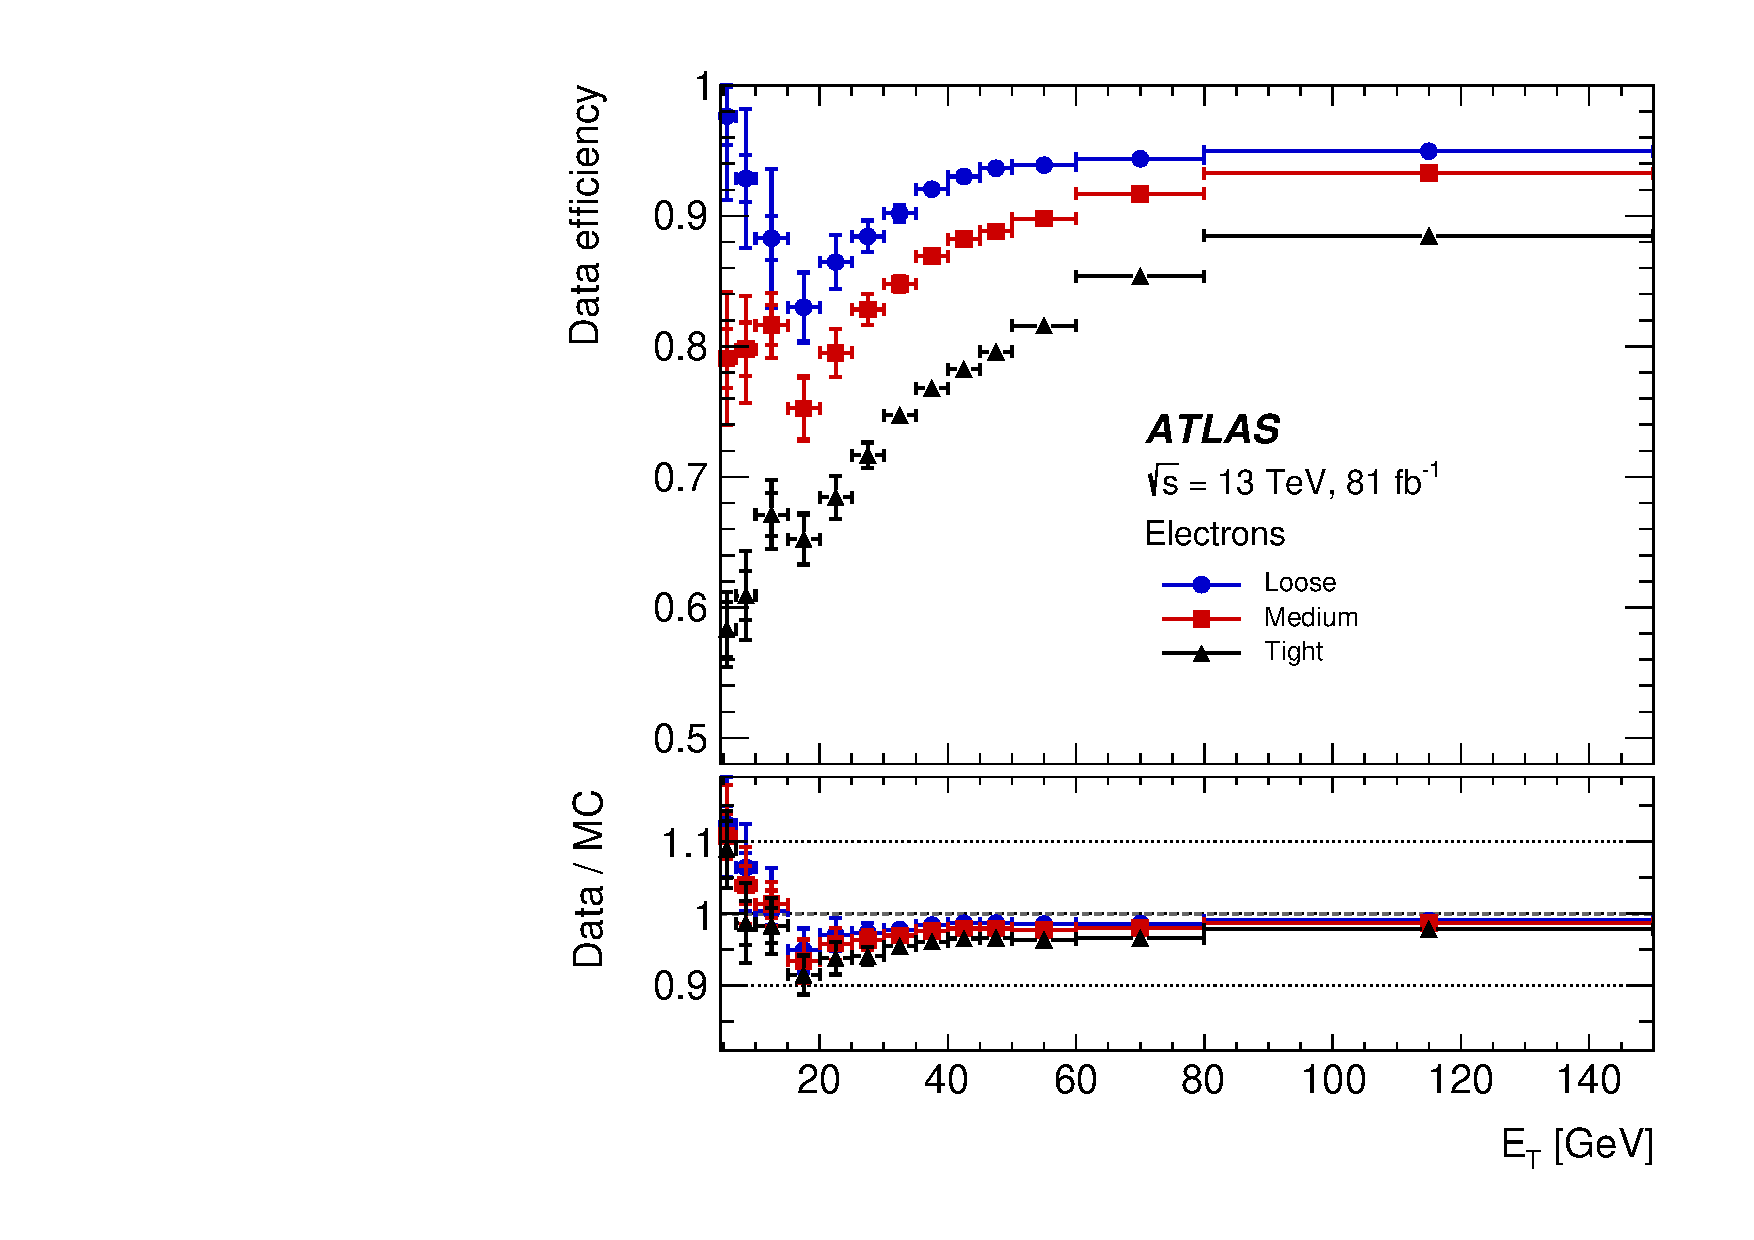
\includegraphics[width=0.79\textwidth]{figures/methods/electron_id_et.pdf}
      \caption{Electron identification efficiency in bins of \(E_{\text{T}}\).}
      \label{fig:methods:event-reconstruction:electrons:identification:et}
    \end{subfigure}
    \\
    \begin{subfigure}{1.\textwidth}
      \centering
      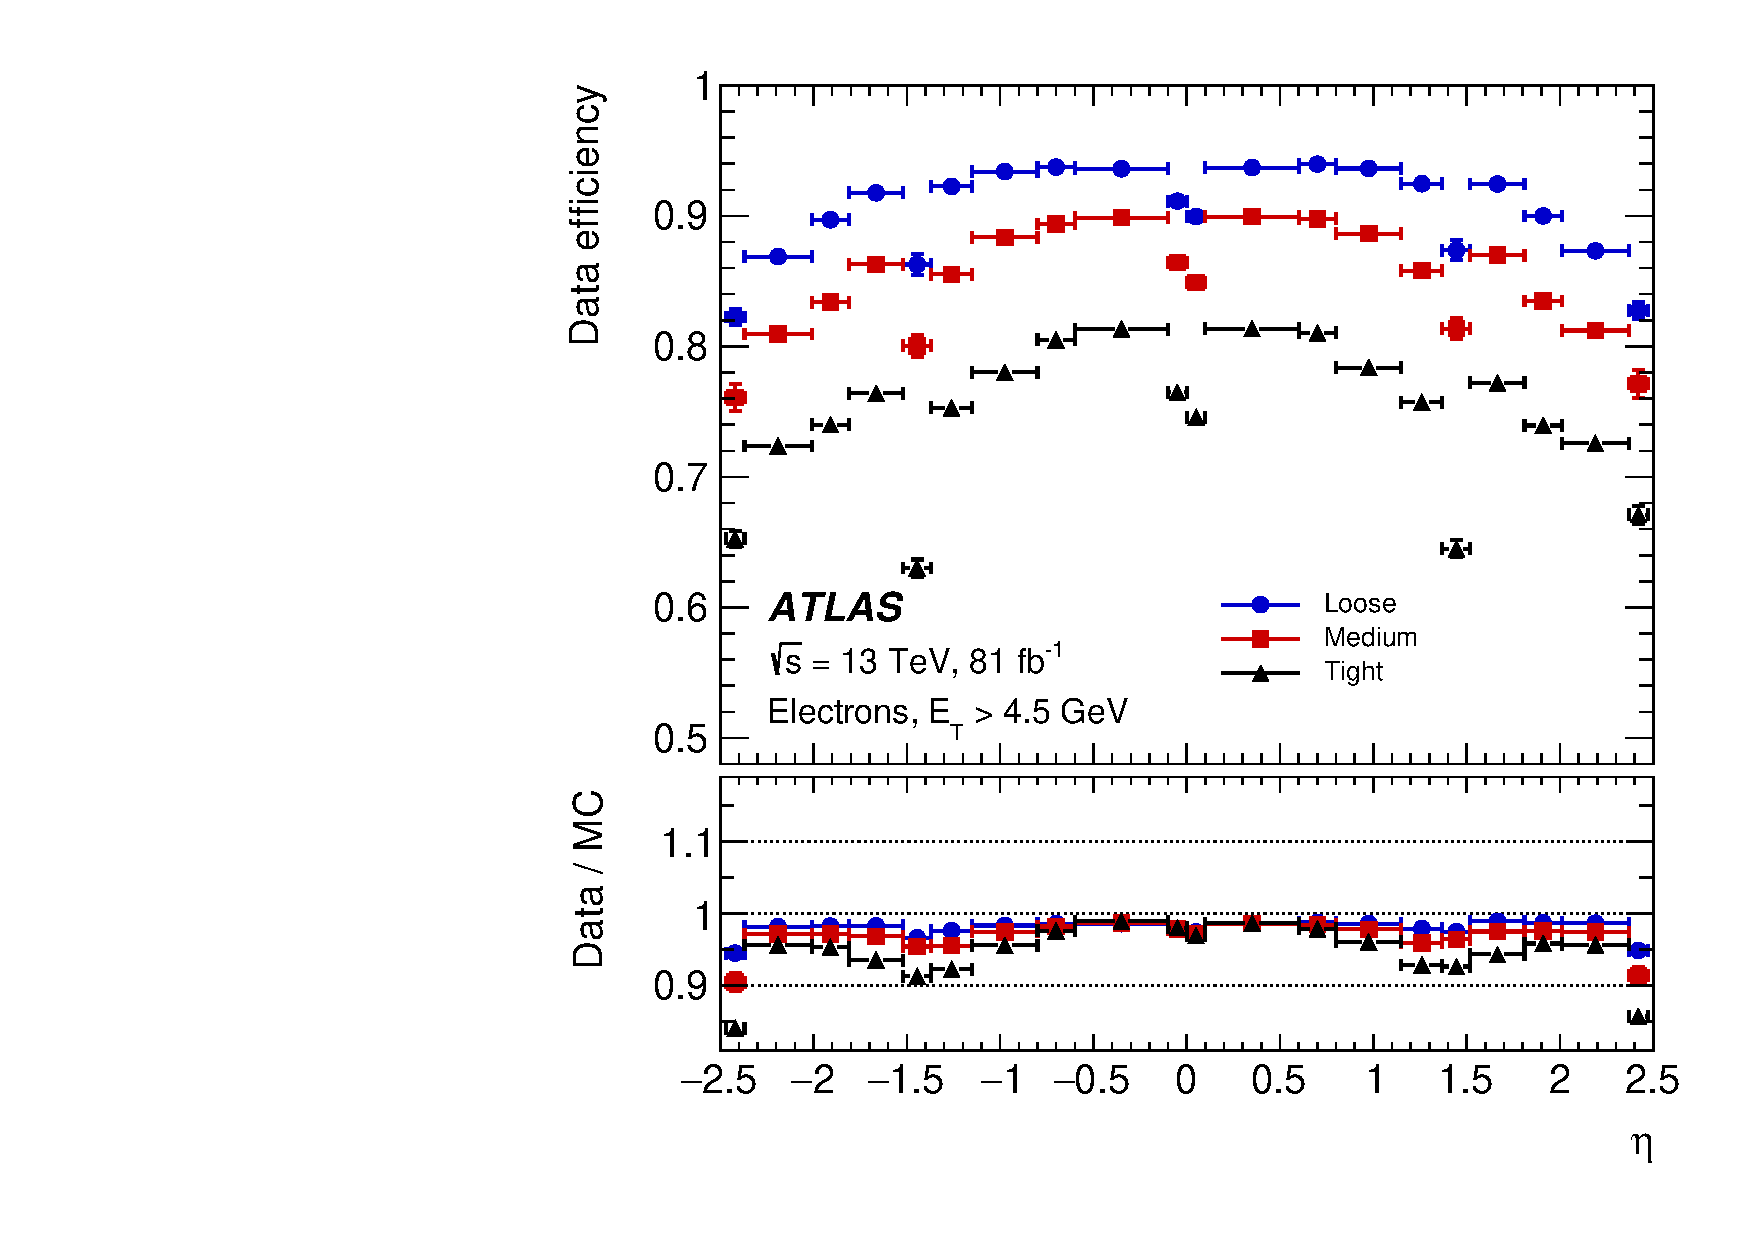
\includegraphics[width=.79\textwidth]{figures/methods/electron_id_eta.pdf}
      \caption{Electron identification efficiency in bins of \(\eta\).}
      \label{fig:methods:event-reconstruction:electrons:identification:eta}
    \end{subfigure}
    \caption{Electron identification efficiencies for the different operating points \textsc{Loose}, \textsc{Medium}, and \textsc{Tight}. Figures reproduced from Ref.~\cite{EGAM-2018-01}.}
    \label{fig:methods:event-reconstruction:electrons:identification}
\end{figure}

\subsubsection{Electron isolation}
The electron isolation algorithm provides additional information to discriminate between electrons from signal processes and background-like objects. Typically, the latter are characterised by comparatively larger activity in an area of \(\eta \times \varphi\) surrounding the electron candidate.
The amount of activity in the vicinity of the electron is quantified by variables summing the transverse energy of clusters or transverse momenta of tracks in a cone of radius \(\Delta R\) around the direction of the electron, excluding the electron itself.

Two types of variables are defined.
\begin{itemize}
	\item The track isolation variable \(p_{T}^{\text{varcone}, 0.2}\) is defined as the sum of the transverse momenta of all tracks in a cone of variable size \(R = \min \{0.2, \SI{10}{\giga\electronvolt} / E_{\text{T}}\}\) around the direction of the electron candidate with transverse energy \(E_{\text{T}}\).
	The \(p_{T}^{\text{varcone}, 0.3}\) variable is defined similarly.
	\item The calorimeter \(E_{T}^{\text{cone}, 0.2}\) isolation variable is defined as the sum of the transverse energies of all calorimeter cells, which are calibrated to the electromagnetic cell, in a cone with fixed size \(R=0.2\) around the electron.
\end{itemize}

Various electron isolation OPs are defined. These can be based either on targeting a fixed value of the isolation efficiency dependent on \(E_{\text{T}}\) and uniform in \(\eta\) (``Gradient'') or by imposing fixed requirements on the value of the isolation variable (``Fixed Cut'').

The electron isolation efficiency for various OPs in bins of \pt and \(\eta\) is shown in \Cref{fig:methods:event-reconstruction:electrons:isolation}.
\begin{figure}[htbp]
    \centering
    \begin{subfigure}{1.\textwidth}
      \centering
      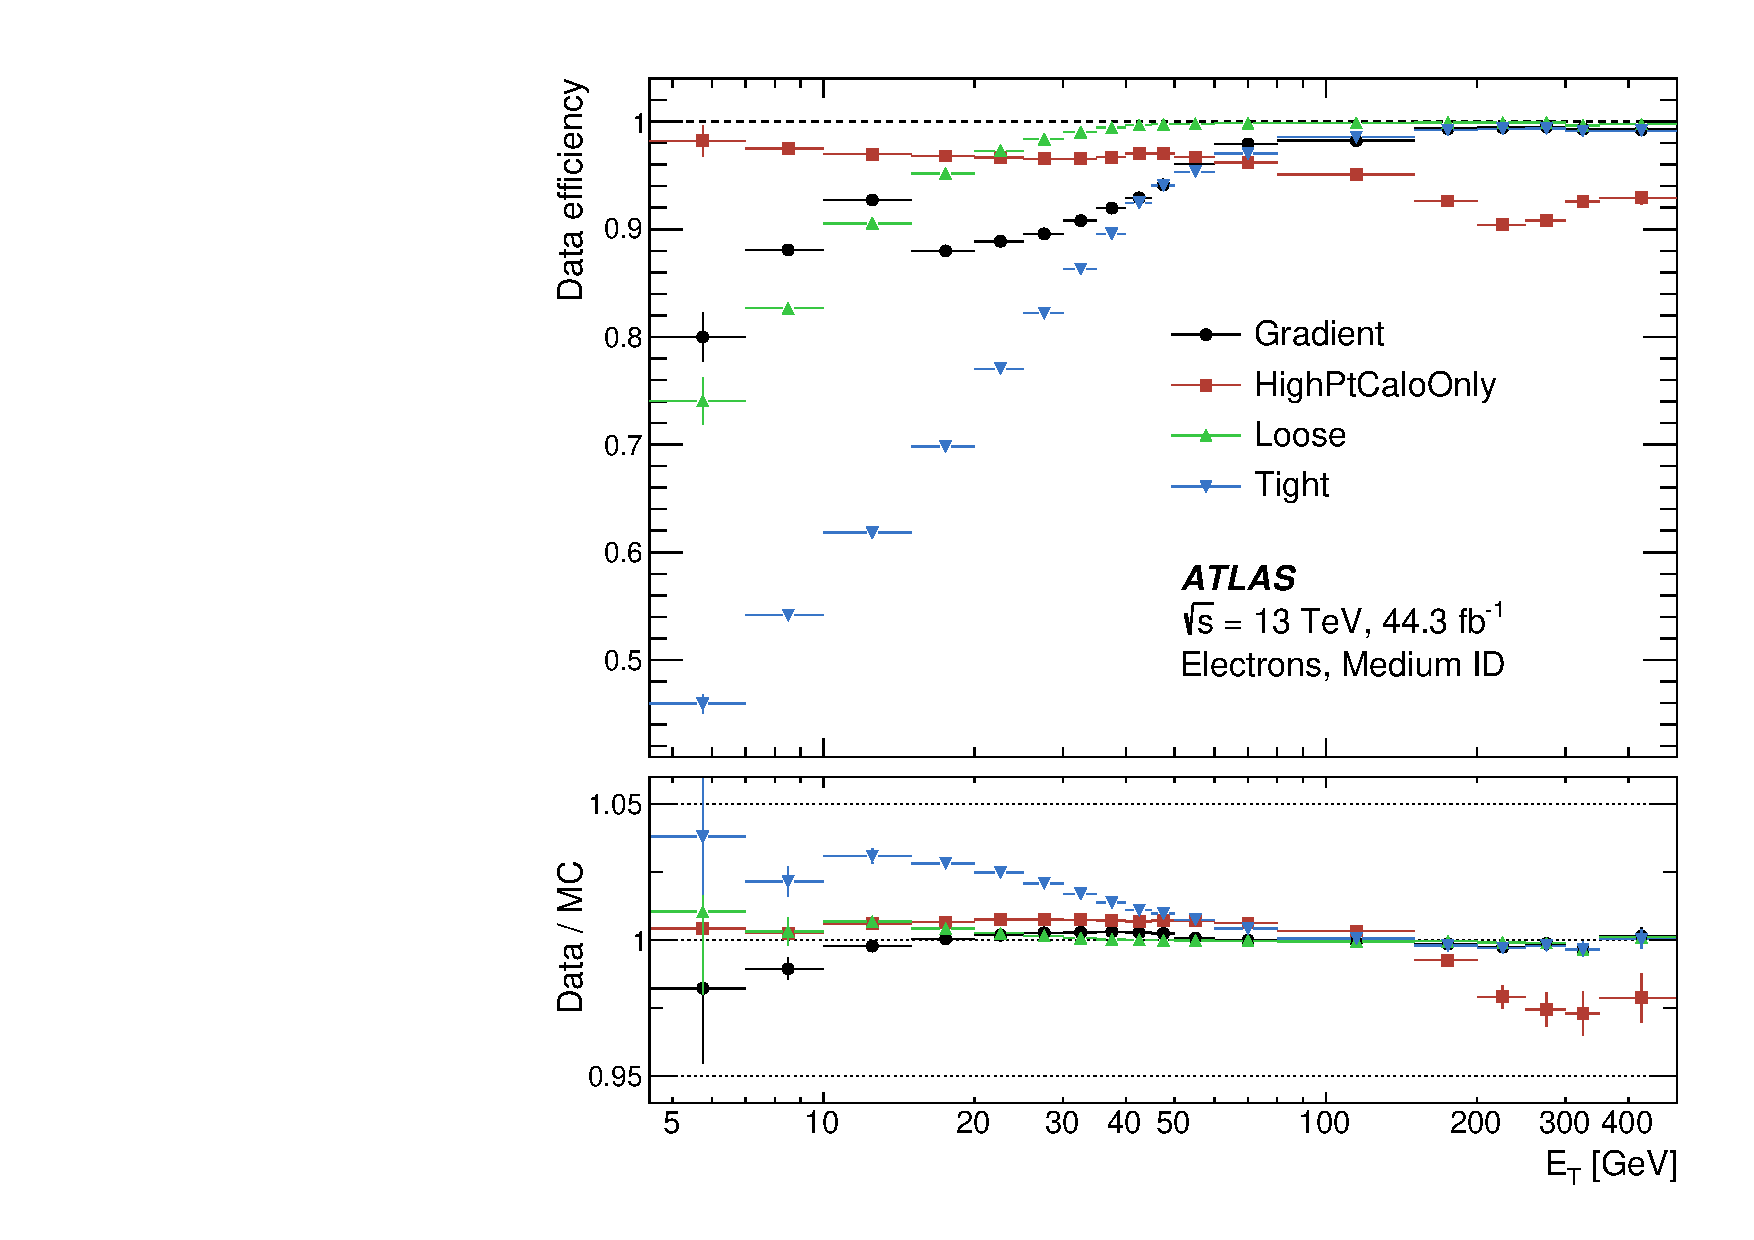
\includegraphics[width=0.79\textwidth]{figures/methods/electron_iso_et.pdf}
      \caption{Electron isolation efficiency in bins of \(E_{\text{T}}\).}
      \label{fig:methods:event-reconstruction:electrons:isolation:et}
    \end{subfigure}
    \\
    \begin{subfigure}{1.\textwidth}
      \centering
      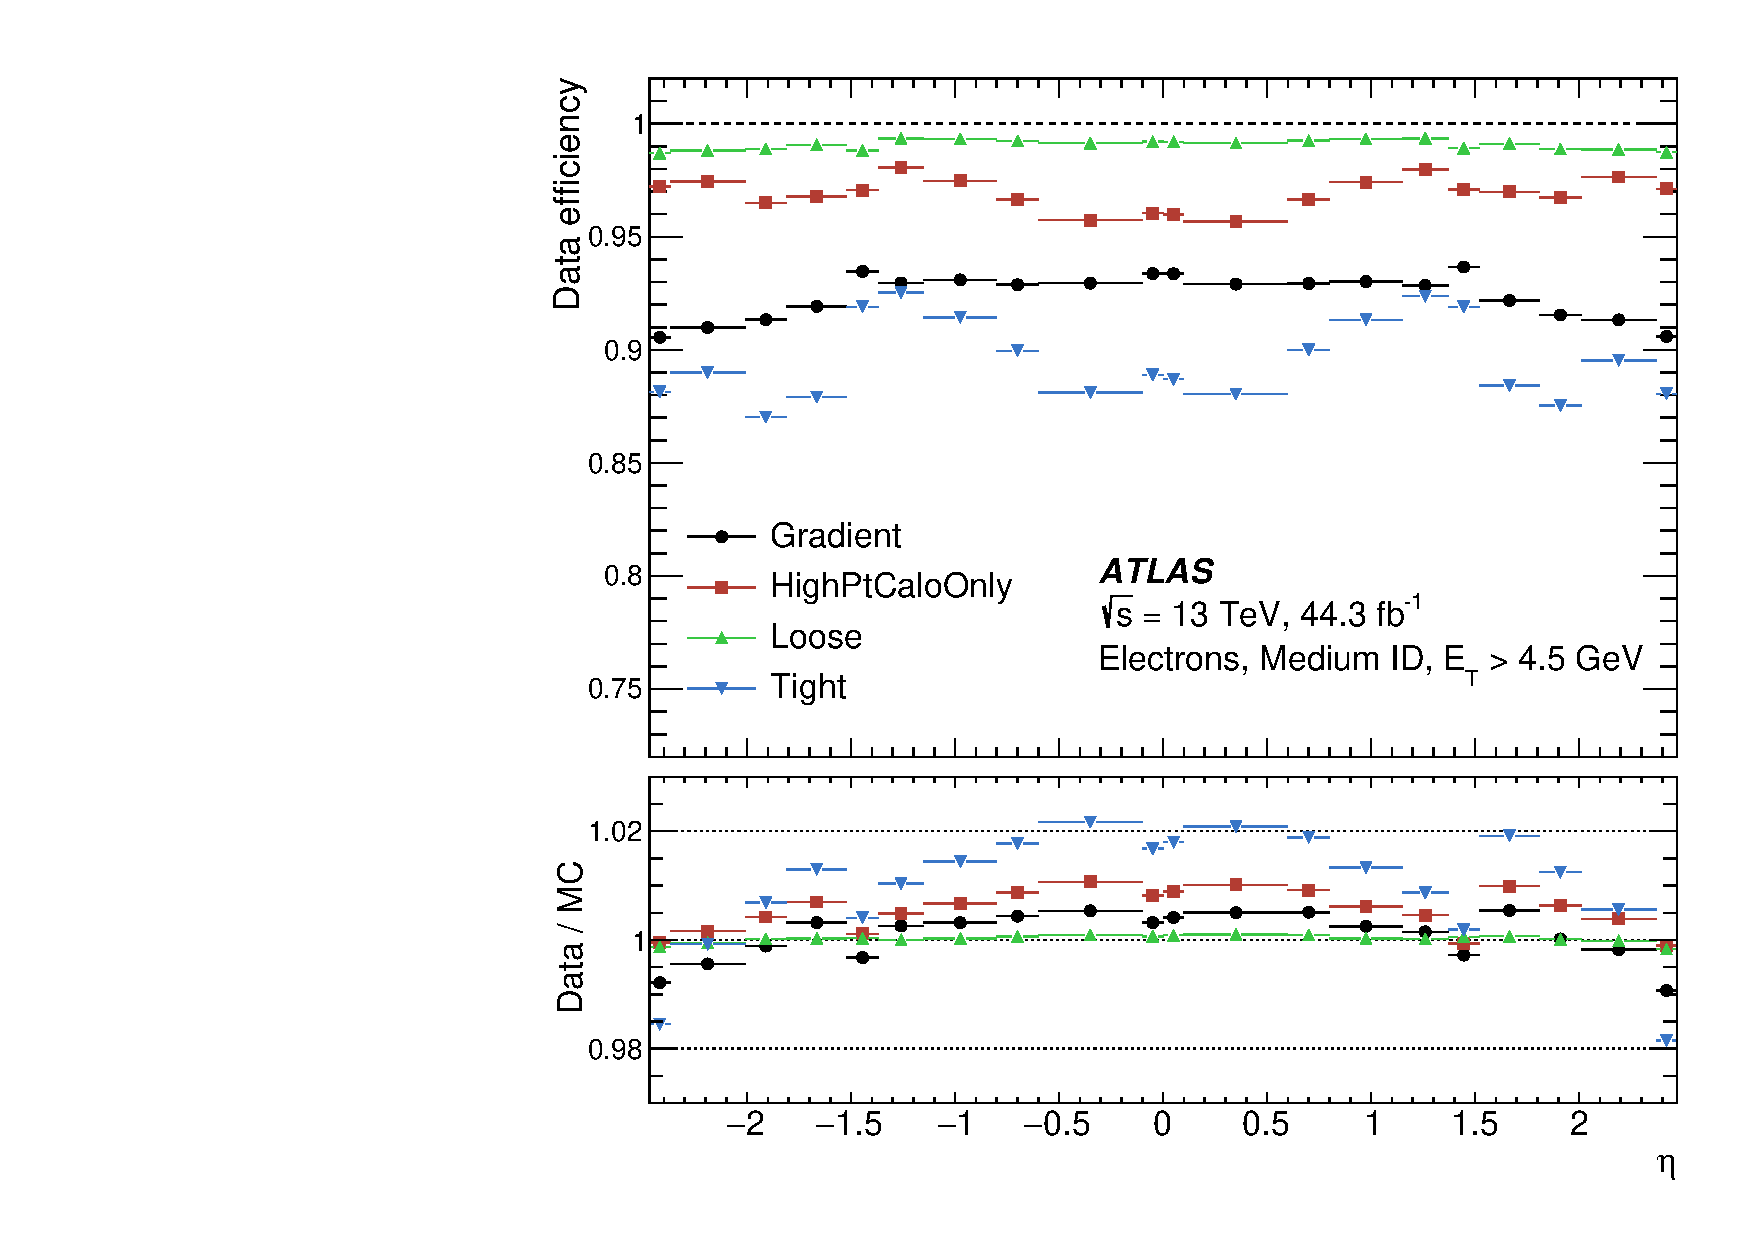
\includegraphics[width=.79\textwidth]{figures/methods/electron_iso_eta.pdf}
      \caption{Electron isolation efficiency in bins of \(\eta\).}
      \label{fig:methods:event-reconstruction:electrons:isolation:eta}
    \end{subfigure}
    \caption{Electron isolation efficiencies for the fixed cut OPs ``Loose'', ``Tight'', and ``HighPtCaloOnly'', as well as for the ``Gradient'' OP. Figures reproduced from Ref.~\cite{EGAM-2018-01}.}
    \label{fig:methods:event-reconstruction:electrons:isolation}
\end{figure}


\subsection{Muons}
\label{sec:methods:event-reconstruction:muons}
Muons traversing the ATLAS detector leave a track in the ID and the MS, as they pass the calorimeters with only minimal energy loss. The muon trajectory is reconstructed independently in the ID and the MS. Then, the two measurements are combined, potentially supplemented with calorimeter information, to form muon candidates.

The performance of the muon reconstruction, identification, and isolation algorithms is evaluated in data and simulated MC samples using muons from \HepProcess{\PZ \to \Pgmm \Pgmp} and \HepProcess{\PJgy \to \Pgmm \Pgmp} decays.

\subsubsection{Muon reconstruction}
The muon reconstruction~\cite{PERF-2015-10,ATLAS-CONF-2020-030} is performed separately in the ID and the MS. While the muon reconstruction in the ID is identical to that of other charged particles (c.f. \Cref{sec:methods:event-reconstruction:basic}), it based on a combinatorial search algorithm in the MS. The algorithm constructs the track candidates from at least two matching track segments, which are identified in the individual layers of the MS by pattern finding algorithms.

Six types of muons are reconstructed depending on the available sub-detector information and based on different reconstruction algorithms. The reconstructed muon types are combined (CB) muons, silicon-associated forward (SiF) muons, inside-out combined (IO) muons, segment-tagged (ST) muons, calorimeter-tagged (CT) muons and extrapolated (ME) muons.

\begin{itemize}
	\item \textbf{Combined muons} are reconstructed with an ``outside-in'' approach by matching MS tracks to ID tracks and performing a global re-fit of the hits from both the ID and MS sub-detectors to construct the muon candidate. The global fit procedure allows for addition or removal of MS hits from the track to improve the fit quality. Typically, CB muon candidates have the highest muon purity among all muon definitions.
	\item \textbf{Inside-out combined muons} complement the reconstruction of CB muons by an ``inside-out'' approach, in which ID tracks are extrapolated outward and matched to MS tracks while taking into account the energy loss in the calorimeters.
	\item \textbf{Silicon-associated forward muons} are a subset of CB muons, which are reconstructed for \(\abs{\eta} > 2.5\) by combining MS tracks with short track segments reconstructed from hits in the pixel and SCT detectors.
	\item \textbf{Segment-tagged muons} are reconstructed from muons with either insufficient momentum to traverse the full MS or which fall in regions with reduced acceptance. They are based on ID tracks which are extrapolated to at least one local track segment in an MDT or CSC detector.
	\item \textbf{Calorimeter-tagged muons} are reconstructed from muons, whose trajectory only extends to the calorimeters. They are based on ID tracks which are matched to an energy deposit in the calorimeters compatible with a minimum-ionising particle. CT muons are designed to recover acceptance in the region \(\abs{\eta} < 0.1\), where the MS is only partially instrumented, but have the lowest purity among all muon types.
	\item \textbf{Extrapolated muons} are reconstructed using only the track reconstructed in the MS, which is required to satisfy a loose requirement of being compatible with originating from the interaction point. They are designed to extend the acceptance for the region \(2.5 < \abs{\eta} < 2.7\), which is not covered by the ID. The parameters of the muon track are defined at the interaction point, taking into account the estimated energy loss of the muon in the calorimeters.
\end{itemize}

The collections of muons used in physics analysis have the overlaps between the different muon types resolved. When two muons share the same ID track, priority is given to CB or IO muons (choosing the type with better fit quality), then to SiF, then to ST, and then to CT muons. When a muon of the previously mentioned types overlaps with an ME muon, the overlap is resolved by selecting the track with a better fit quality and a larger number of hits.

\subsubsection{Muon identification}
The muon identification algorithms discriminate between prompt muons originating from signal processes and background-like objects. The identification of CB muons is based on three variables
\begin{itemize}
	\item \(q / p\) significance, which is defined as the ratio of \(\abs{(q / p)_{\text{ID}} - (q / p)_{\text{MS}}}\) and \(\sqrt{\sigma(q / p)_{\text{ID}}^2 + \sigma(q / p)_{\text{MS}}^2}\), where \((q / p)_{\text{ID (MS)}}\) is the ratio of the charge and momentum of the muons measured in the ID (MS) and \(\sigma(q / p)_{\text{ID (MS)}}\) is the corresponding resolution,
	\item residual between the momentum measurements in the ID and MS divided by the transverse momenta of the combined track \(\rho' = \abs{p_{\text{T}, \text{ID}} - p_{\text{T}, \text{MS}}} / \pt^{\text{comb}}\),
	\item normalised \(\chi^2\) of the combined track fit.
\end{itemize}

Five OPs are defined based on these variables, which address the specific needs of a wide range physics analyses, including \textsc{Loose}, \textsc{Medium}, \textsc{Tight}, \textsc{LowPT}, and \textsc{HighPT} OPs.
Out of these definitions, \textsc{Loose} and \textsc{Medium} muons are considered in the searches for dark matter presented in this dissertation.
\begin{itemize}
	\item \textsc{Loose} muons are identified from all muon types. CB muons are required to have at least three hits in at least two MDT layers, except for muons in the sparsely instrumented region \(\abs{\eta} < 0.1\)). ME muons are required to have hits in at least three MDT or CSC layers. ST and CT muons are considered in the region \(\abs{\eta} < 0.1\). Contamination due to hadrons misidentified as muons is suppressed by requiring a \(q / p\) significance less than seven and imposing a loose selection on the compatibility between ID and MS momentum measurements.
	\item \textsc{Medium} muons are identified only from CB or ME muons, which satisfy all requirements defined for the \textsc{Loose} OP.
	% \item \textsc{Tight} muons are identified CB muons with hits in at least two layers of the MS. They satisfy all selection criteria of the \textsc{Medium} OP. In addition, the normalised \(\chi^2\) of the combined track fit is required to be smaller than eight and a two-dimensional \pt-dependent requirement on \(\rho'\) and \(\text{sig}_{q / p}\) is imposed to improve background rejection.
	% \item \textsc{LowPT} muons are identified from CB and IO muons. Muons reconstructed only by the IO algorithm are required to be verified by independent reconstruction also by the ST algorithm. Further selection requirements are imposed to reject light hadron decays.
	% \item \textsc{HighPT} muons are identified from CB muons with at least three hits in three layers of the MS. This OP is optimised for muons with transverse momenta above \SI{100}{\giga\electronvolt}.
\end{itemize}

The muon identification efficiency in bins of \pt and two-dimensional binning in \(\eta\)-\(\varphi\) are shown in \Cref{fig:methods:event-reconstruction:muons:identification}. The efficiency for the \textsc{Loose} and \textsc{Medium} OPs exceeds \SI{98}{\percent} for muons with \(0.1 < \abs{\eta} < 2.5\). The agreement between collision data and detector simulation is very good, with average differences at the level of \SI{0.5}{\percent}.

\begin{figure}[htbp]
    \centering
    \begin{subfigure}{1.\textwidth}
      \centering
      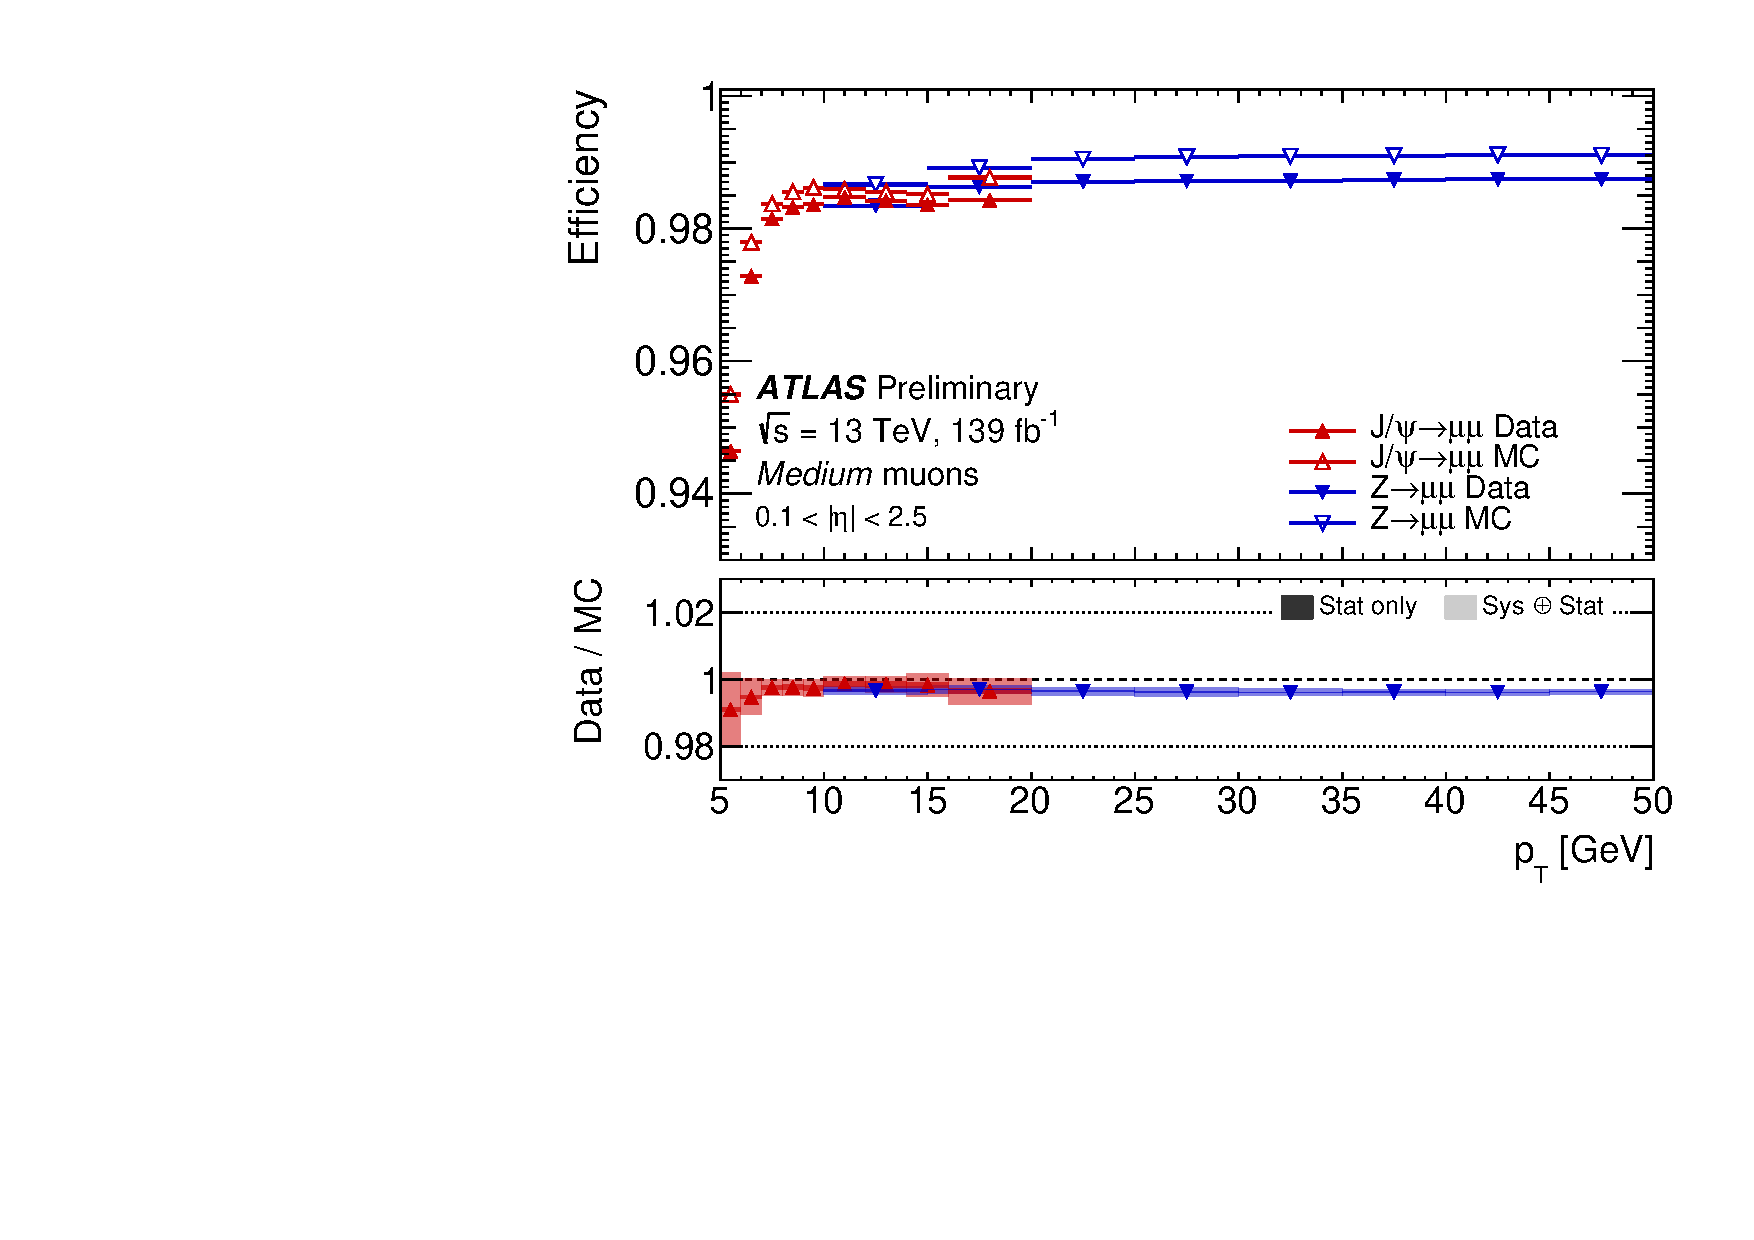
\includegraphics[width=0.95\textwidth]{figures/methods/muon_id_pt.pdf}
      \caption{Muon reconstruction and identification efficiencies in bins of \pt for muons with \(0.1 < \abs{\eta} < 2.5\). The bottom panel shows the ratio of the measured to predicted efficiencies, with statistical and systematic uncertainties~(shaded boxes).}
      \label{fig:methods:event-reconstruction:muons:identification:pt}
    \end{subfigure}
    \\
    \begin{subfigure}{1.\textwidth}
      \centering
      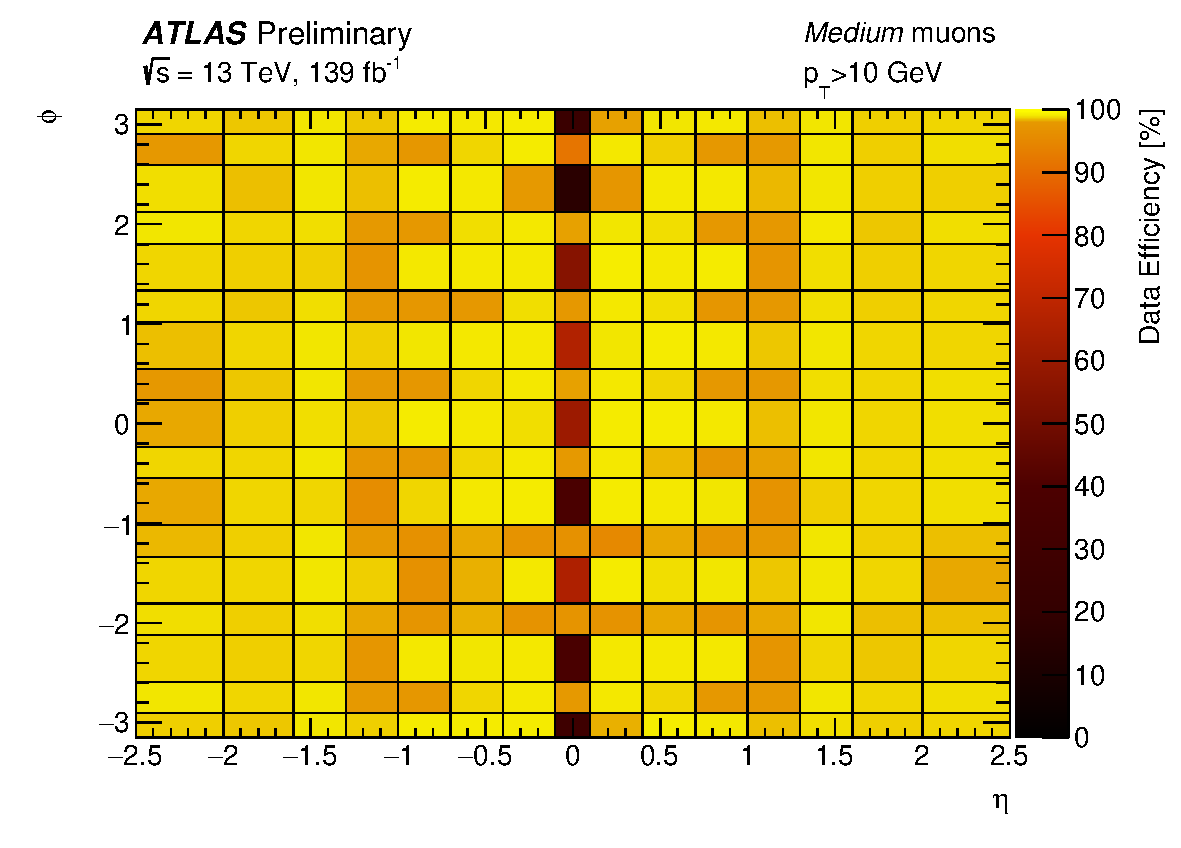
\includegraphics[width=.95\textwidth]{figures/methods/muon_id_eta.pdf}
      \caption{reconstruction and identification efficiencies measured in collision data in bins of \(\eta\)-\(\varphi\) for muons with \(\pt > \SI{10}{\giga\electronvolt}\) as a function of \(\eta\) and \(\varphi\).}
      \label{fig:methods:event-reconstruction:muons:identification:etaphi}
    \end{subfigure}
    \caption{Muon reconstruction and identification efficiencies for \textsc{Medium} muons with \(\pt > \SI{10}{\giga\electronvolt}\). Figures reproduced from Ref.~\cite{ATLAS-CONF-2020-030}.}
    \label{fig:methods:event-reconstruction:muons:identification}
\end{figure}

Additional requirements are imposed on the impact parameters of the muon track to associate the muon candidates with the PV and thereby reject muons originating from cosmic rays, pile-up interactions, or muons originating from secondary hadron decays. The shortest distance from the muon track to the primary vertex in a longitudinal projection is required to satisfy \(\abs{z_{0}} \sin \theta < \SI{0.5}{\milli\meter}\) and the transverse impact parameter significance is required to satisfy \(\abs{d_{0}} / \sigma(d_{0}) < 3\).


\subsubsection{Muon isolation}
Similar to the case of electrons, specific isolation requirements allow for better discrimination between muons from signal processes and background-like objects. Track-based and calorimeter-based isolation variables are employed.
\begin{itemize}
	\item The track isolation variable \(p_{T}^{\text{varcone}, 0.2}\) is defined as the sum of the transverse momenta of all tracks in a cone of variable size \(R = \min \{0.2, \SI{10}{\giga\electronvolt} / \pt\}\) around the direction of the muon with transverse momentum \pt.
	The \(p_{T}^{\text{varcone}, 0.3}\) variable is defined similarly.
	\item The calorimeter \(E_{T}^{\text{cone}, 0.2}\) isolation variable is defined as the sum of the transverse energies of all calorimeter clusters in a cone with fixed size \(R=0.2\) around the muon.
\end{itemize}

Several OPs can be defined using these variables, which either apply a fixed cut on the selected isolation variable or target a specific value of the isolation efficiency in dependence on the muon \pt.

\Cref{fig:methods:event-reconstruction:muons:isolation} shows the muon isolation efficiency for the \textsc{Loose} and \textsc{Tight} fixed cut OPs in bins of \pt.
\begin{figure}[htbp]
    \centering
    \begin{subfigure}{.49\textwidth}
      \centering
      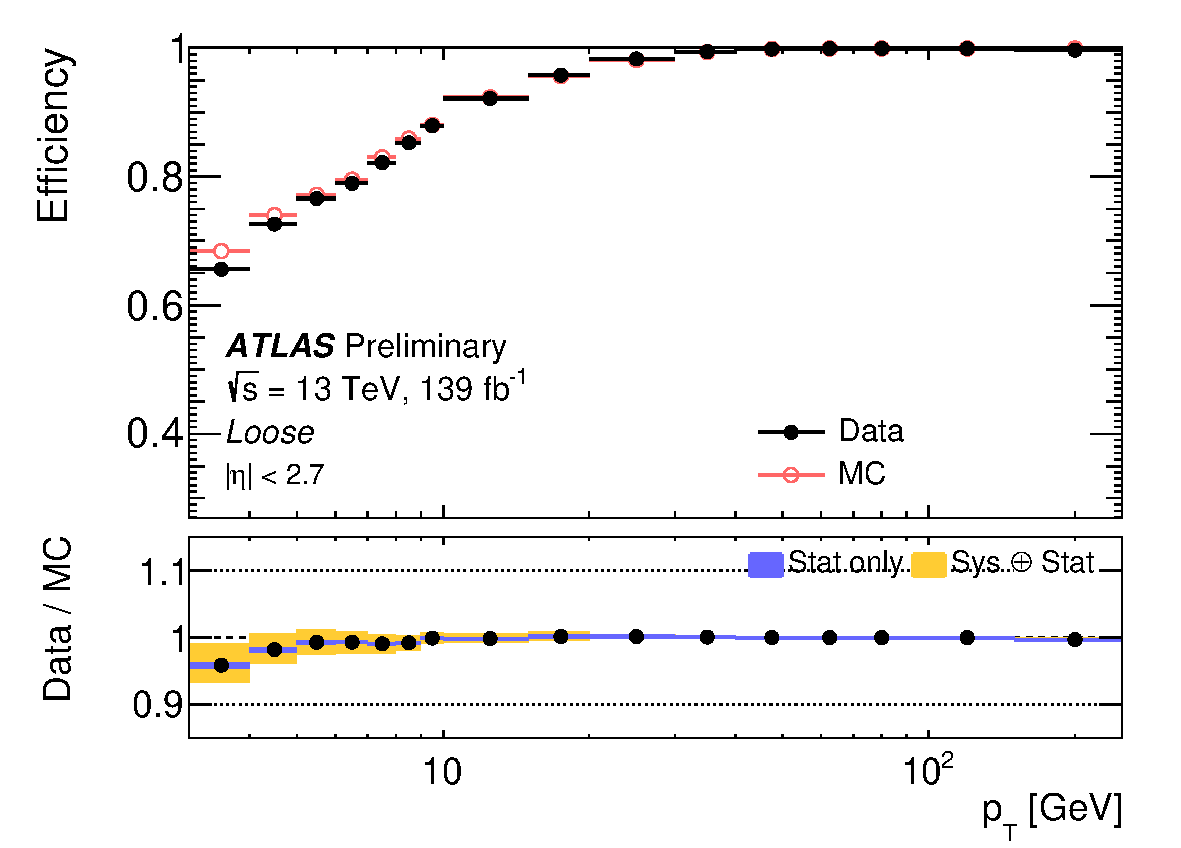
\includegraphics[width=1.\textwidth]{figures/methods/muon_iso_loose.pdf}
      \caption{\textsc{Loose} OP}
      \label{fig:methods:event-reconstruction:muons:isolation:loose}
    \end{subfigure}
    \begin{subfigure}{.49\textwidth}
      \centering
      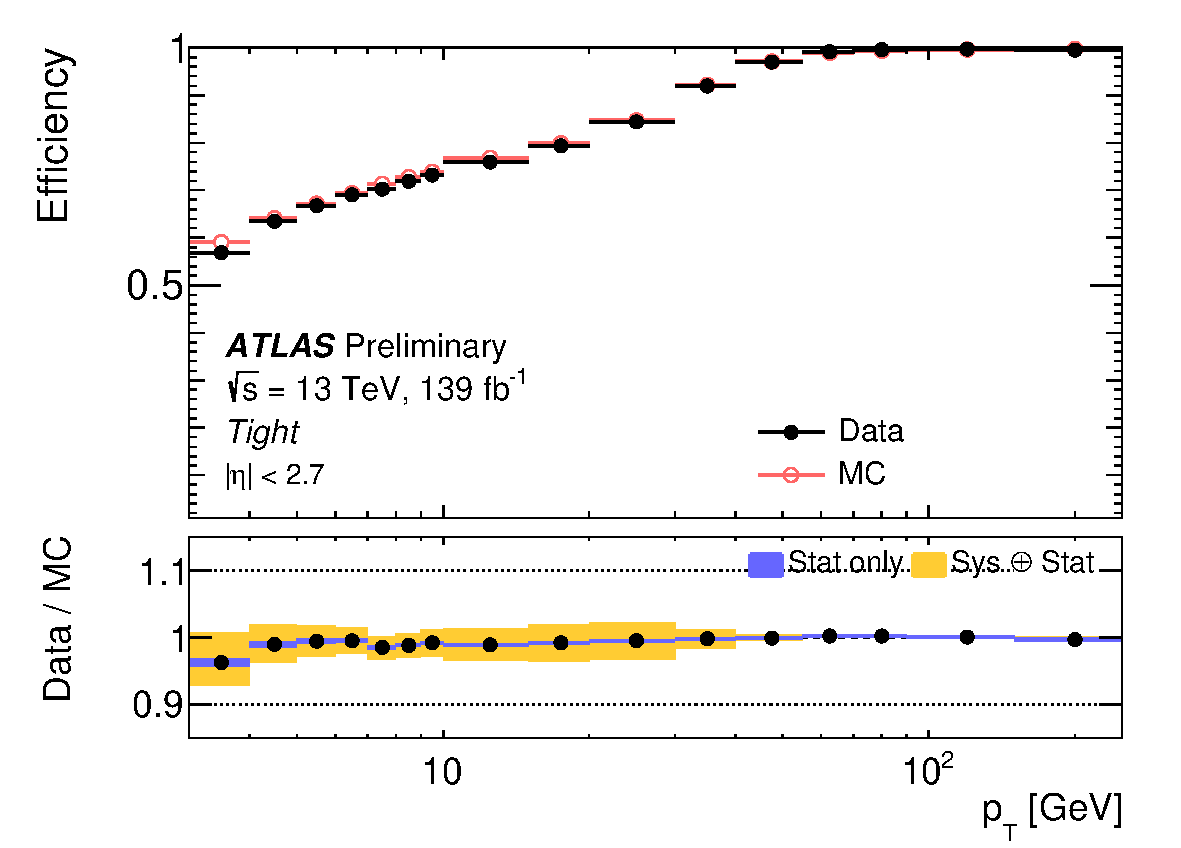
\includegraphics[width=1.\textwidth]{figures/methods/muon_iso_tight.pdf}
      \caption{\textsc{Tight} OP}
      \label{fig:methods:event-reconstruction:muons:isolation:tight}
    \end{subfigure}
    \caption{Muon isolation efficiency in bins of \pt for the \textsc{Loose} and \textsc{Tight} fixed cut OPs. Figures reproduced from Ref.~\cite{ATLAS-CONF-2020-030}.}
    \label{fig:methods:event-reconstruction:muons:isolation}
\end{figure}


\subsection{Jets}
\label{sec:methods:event-reconstruction:jets}
Jets are collimated and localised sprays of particles, which can be reconstructed using jet algorithms (c.f. \Cref{sec:pp:jets}). The \antikt algorithm is used to build jets from topological clusters in the calorimeters, tracks in the ID or stable particles defined by MC event generators. Various radius parameters are used to define in the jet reconstruction, ranging from \(0.2\), \(0.4\), to \(1.0\), including definitions of \pt-dependent radius parameters.
Jets are essential for analyses targeting hadronic final states because they allow associating detector measurements with the parton shower initiated by a single final-state parton.

Jets on detector-level can be built from the energy deposits in the calorimeter, referred to as calorimeter jets or simply jets, or from ID tracks of charged particles, referred to as track jets. While calorimeter jets have a better energy resolution due to the calorimeters also measuring the energy deposits of neutral particles, the track jets have a better spatial resolution due to the intrinsically finer granularity of the ID.
Jets built from stable particles (except muons, neutrinos, and particles from pile-up interactions) in the MC simulation of physics processes are referred to as truth jets. They are used as a reference for the jets reconstructed from detector information in performance studies or early optimisation studies of analyses.

In the following, the reconstruction and calibration of calorimeter jets with small radius parameter, calorimeter jets with large radius parameter, and track jets with fixed and variable radius parameters are described.

\subsubsection{Small-radius calorimeter jets}
\label{sec:methods:event-reconstruction:jets:smallr}
Small-radius calorimeter jets are reconstructed from the topological clusters in the calorimeters calibrated to the EM scale using the \antikt algorithm with a radius parameter \(R=0.4\). The energy scale of the reconstructed small-radius jets is calibrated to the scale particles in MC simulations using a sequence of data- and simulation-based calibrations~\cite{PERF-2016-04,JETM-2018-05}.

The jets produced in the hard-scattering process are expected to originate from the primary vertex. Therefore, the jet direction is recalculated to account for the position of the primary vertex in each event. As a result, the spatial resolution of jets is improved, while keeping the jet energy unchanged.

The sequential calibration scheme, which involves five steps, is illustrated in \Cref{fig:methods:event-reconstruction:jets:smallr:calibration}.

\begin{figure}[htbp]
	\centering
	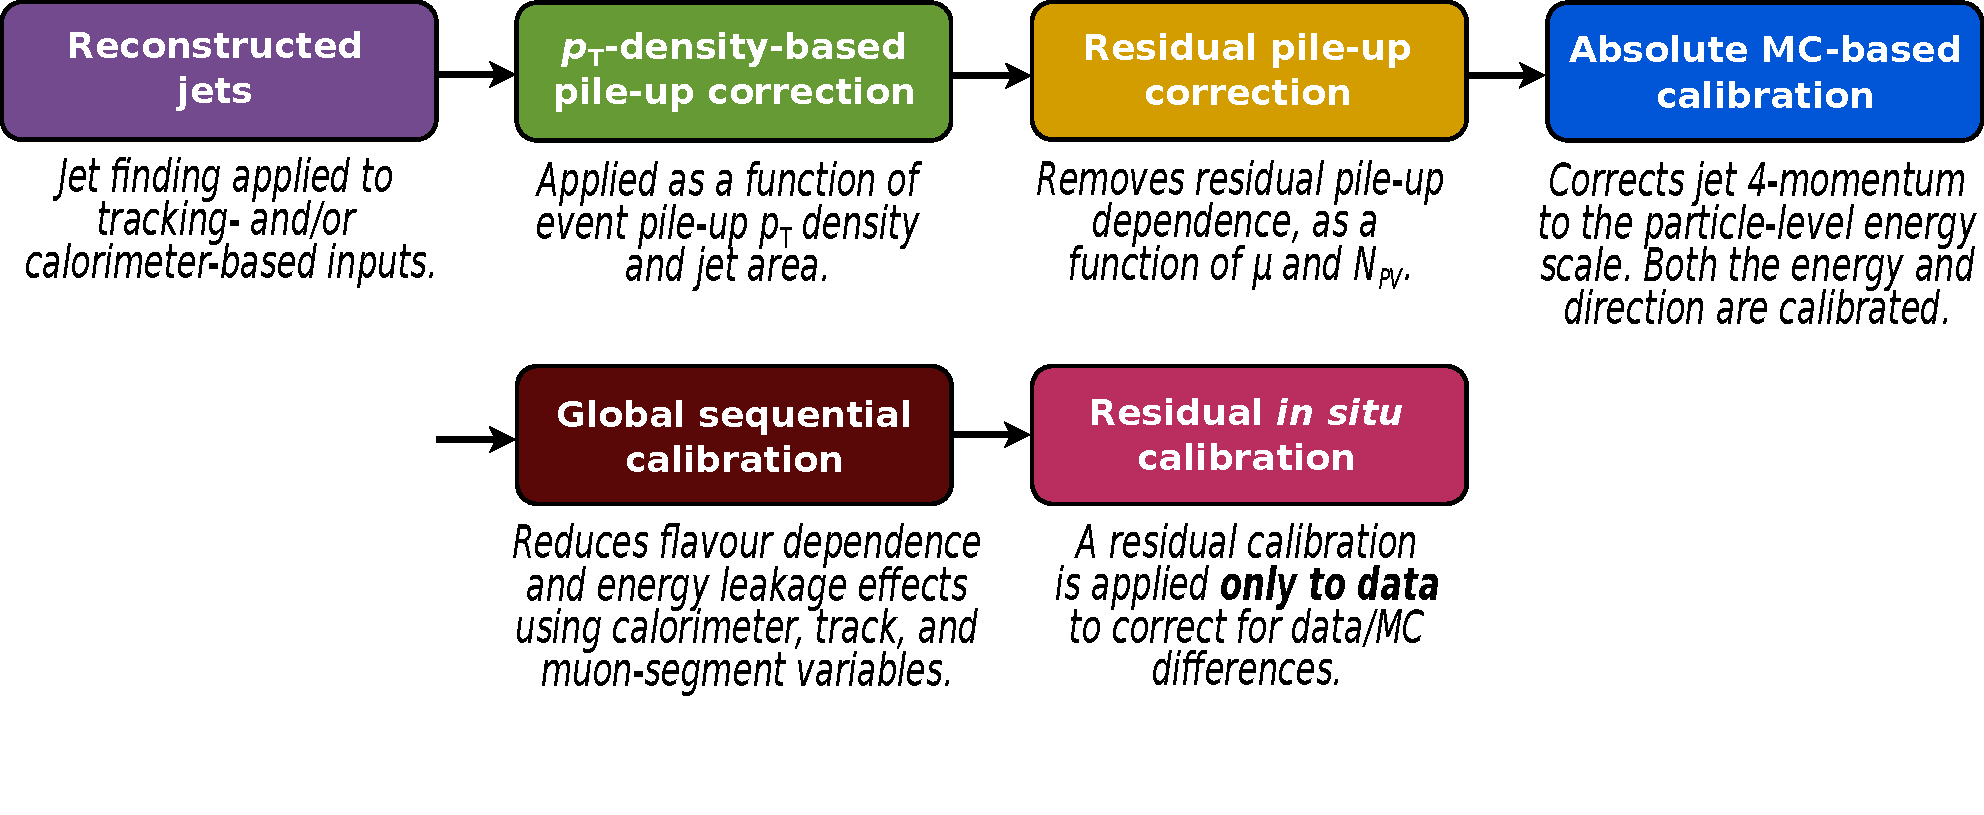
\includegraphics[width=0.95\textwidth]{figures/methods/jet_smallr_calibration.pdf}
	\caption{Stages of jet energy scale calibrations. Each one is applied to the four-momentum of the jet. Figure reproduced from Ref.~\cite{JETM-2018-05}}
	\label{fig:methods:event-reconstruction:jets:smallr:calibration}
\end{figure}

The reconstructed jets first need to be corrected for pile-up by removing the excess energy due to additional \HepProcess{\Pp\Pp} interactions. The pile-up corrections consist of two steps. First, a correction based on the jet area and transverse momentum density of the event is applied. Second, a residual correction derived from MC simulations is applied to remove the remaining dependence on pile-up contributions.
The pile-up corrected jets are calibrated to the particle-level using an MC-based calibration, which corrects their energy and direction. The jet \pt resolution is improved by applying a global sequential calibration. Finally, a residual in-situ calibration is applied to the jets, which corrects for remaining differences between data and simulation.

\begin{enumerate}
	\item \textbf{\pt-density based pile-up correction}. A \pt-density-based subtraction of the event pile-up is performed based on the jet area \(A\) (c.f. ~\Cref{sec:pp:jets}, which is a measure of the susceptibility of the jet to pile-up contributions. The median jet \pt-density \(\rho = \expval{\pt / A}\) is used to estimate the median pile-up contribution in jets. It is calculated from jets in the central lower-occupancy regions \(\abs{\eta} < 2.0\) of the calorimeter, which are reconstructed from topological clusters using the \(k_{\text{T}}\) algorithm with \(R=0.4\) in the rapidity-\(\varphi\) plane.

	\item \textbf{Residual pile-up correction}. After the \pt-density-based correction, some residual dependence on the pile-up activity remains. It is estimated in MC simulations by geometrically matching the reconstructed jets to truth jets within \(\Delta R < 0.3\) and parametrising the difference between the reconstructed jet \(\pt^{\text{reco}}\) and the corresponding truth jet \(\pt^{\text{truth}}\) as a function of the number of reconstructed primary vertices \(N_{\text{PV}}\) and the mean number of interactions per bunch crossing \(\mu\). The former number is a measure of the in-time pile-up, while the latter is a measure for out-of-time pile-up. The residual momentum dependence on \(N_{\text{PV}}\) and \(\mu\) is parametrised as linear functions.

	The jet \pt after both pile-up corrections is
	\(\pt^{\text{PU corr}} = \pt^{\text{reco}} - \rho \times A - \alpha \times (N_{\text{PV}} - 1) - \beta \times \mu\), where \(\pt^{\text{reco}}\) denotes the reconstructed jet \pt before pile-up corrections and \(\alpha, \beta\) are coefficients defined in \(\pt\) and \(\eta\) of the truth jet.

	The dependence of the jet \pt on \(N_{\text{PV}}\) and \(\mu\) is shown in \Cref{fig:methods:event-reconstruction:jets:smallr:pileup}.
\end{enumerate}
\begin{figure}[htbp]
    \centering
    \begin{subfigure}{.49\textwidth}
      \centering
      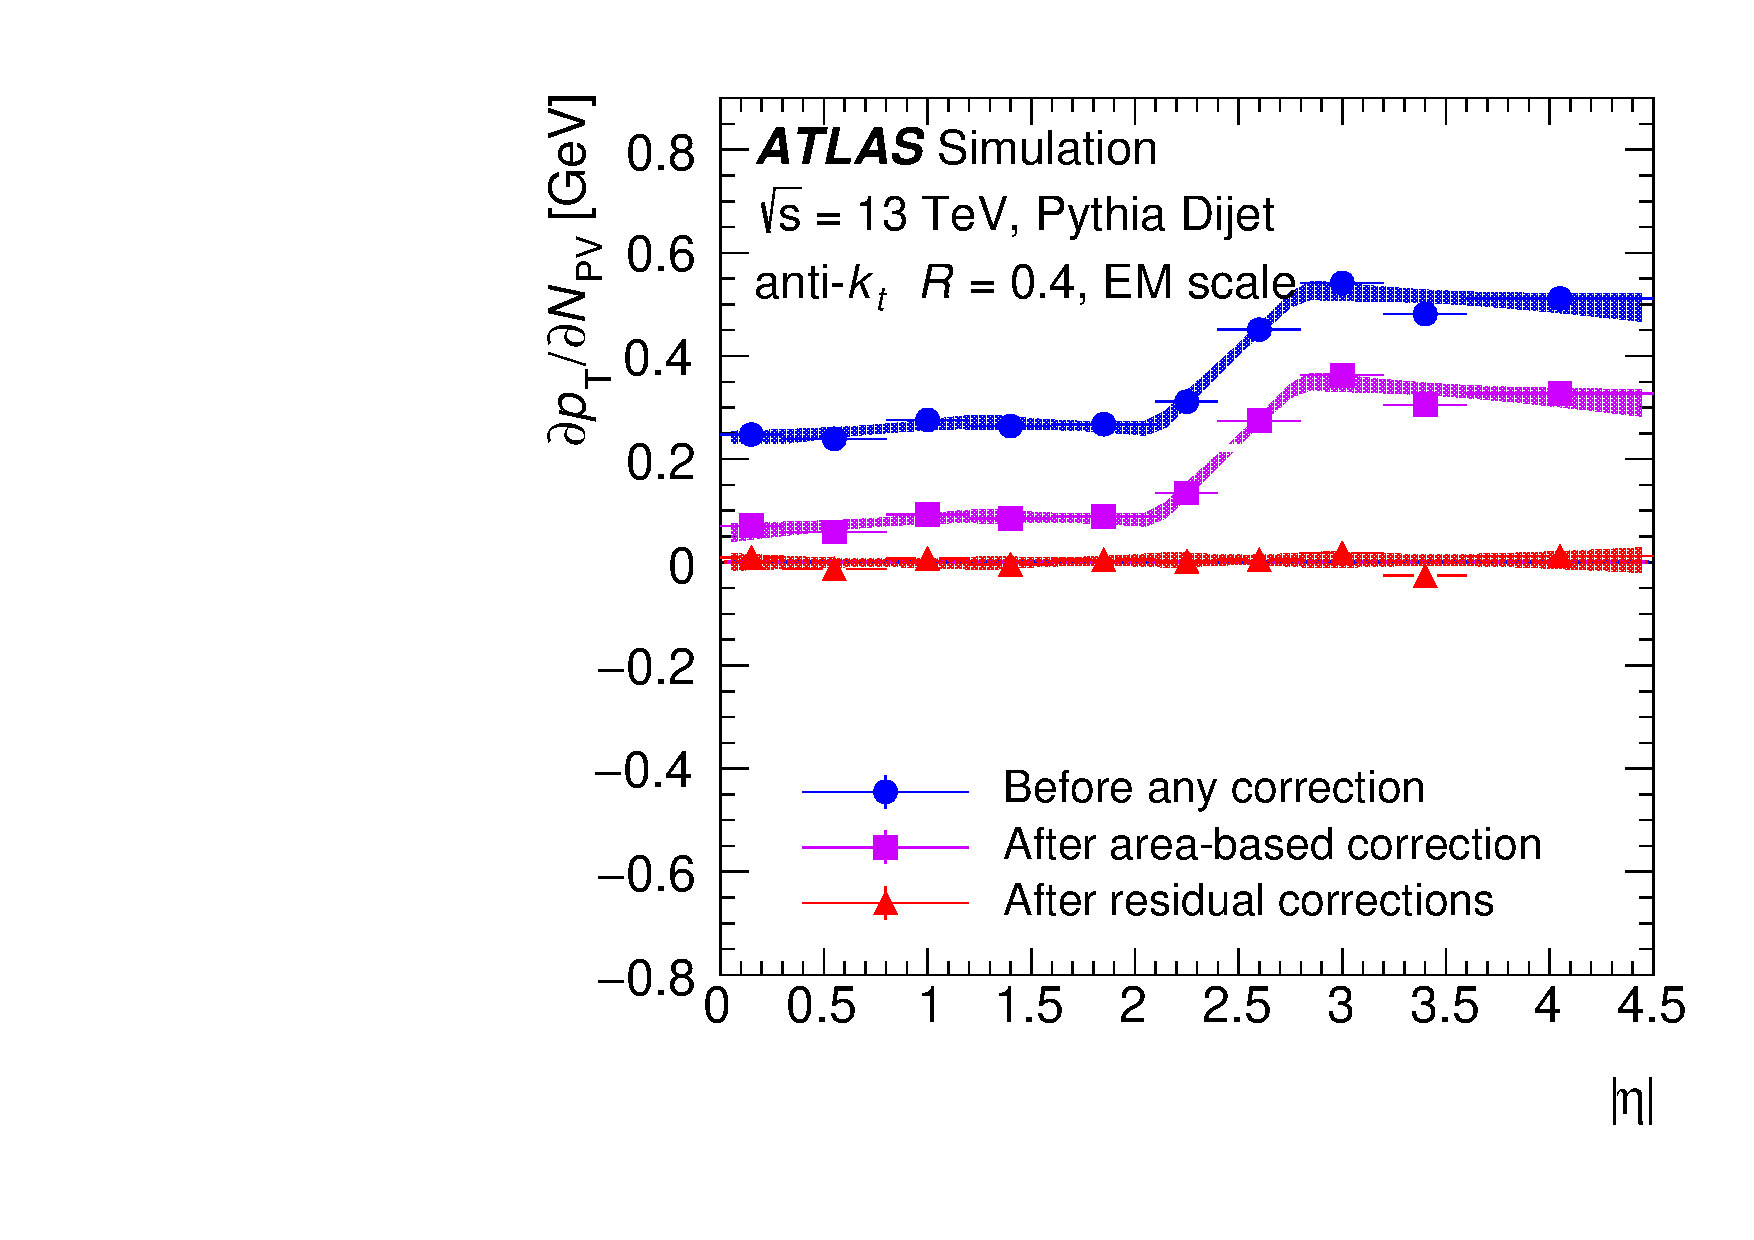
\includegraphics[width=1.\textwidth]{figures/methods/jet_pu-npv.pdf}
      \caption{Dependence of jet \pt on \(N_{\text{PV}}\), averaged over \(\mu\).}
      \label{fig:methods:event-reconstruction:jets:pileup-npv}
    \end{subfigure}
    \begin{subfigure}{.49\textwidth}
      \centering
      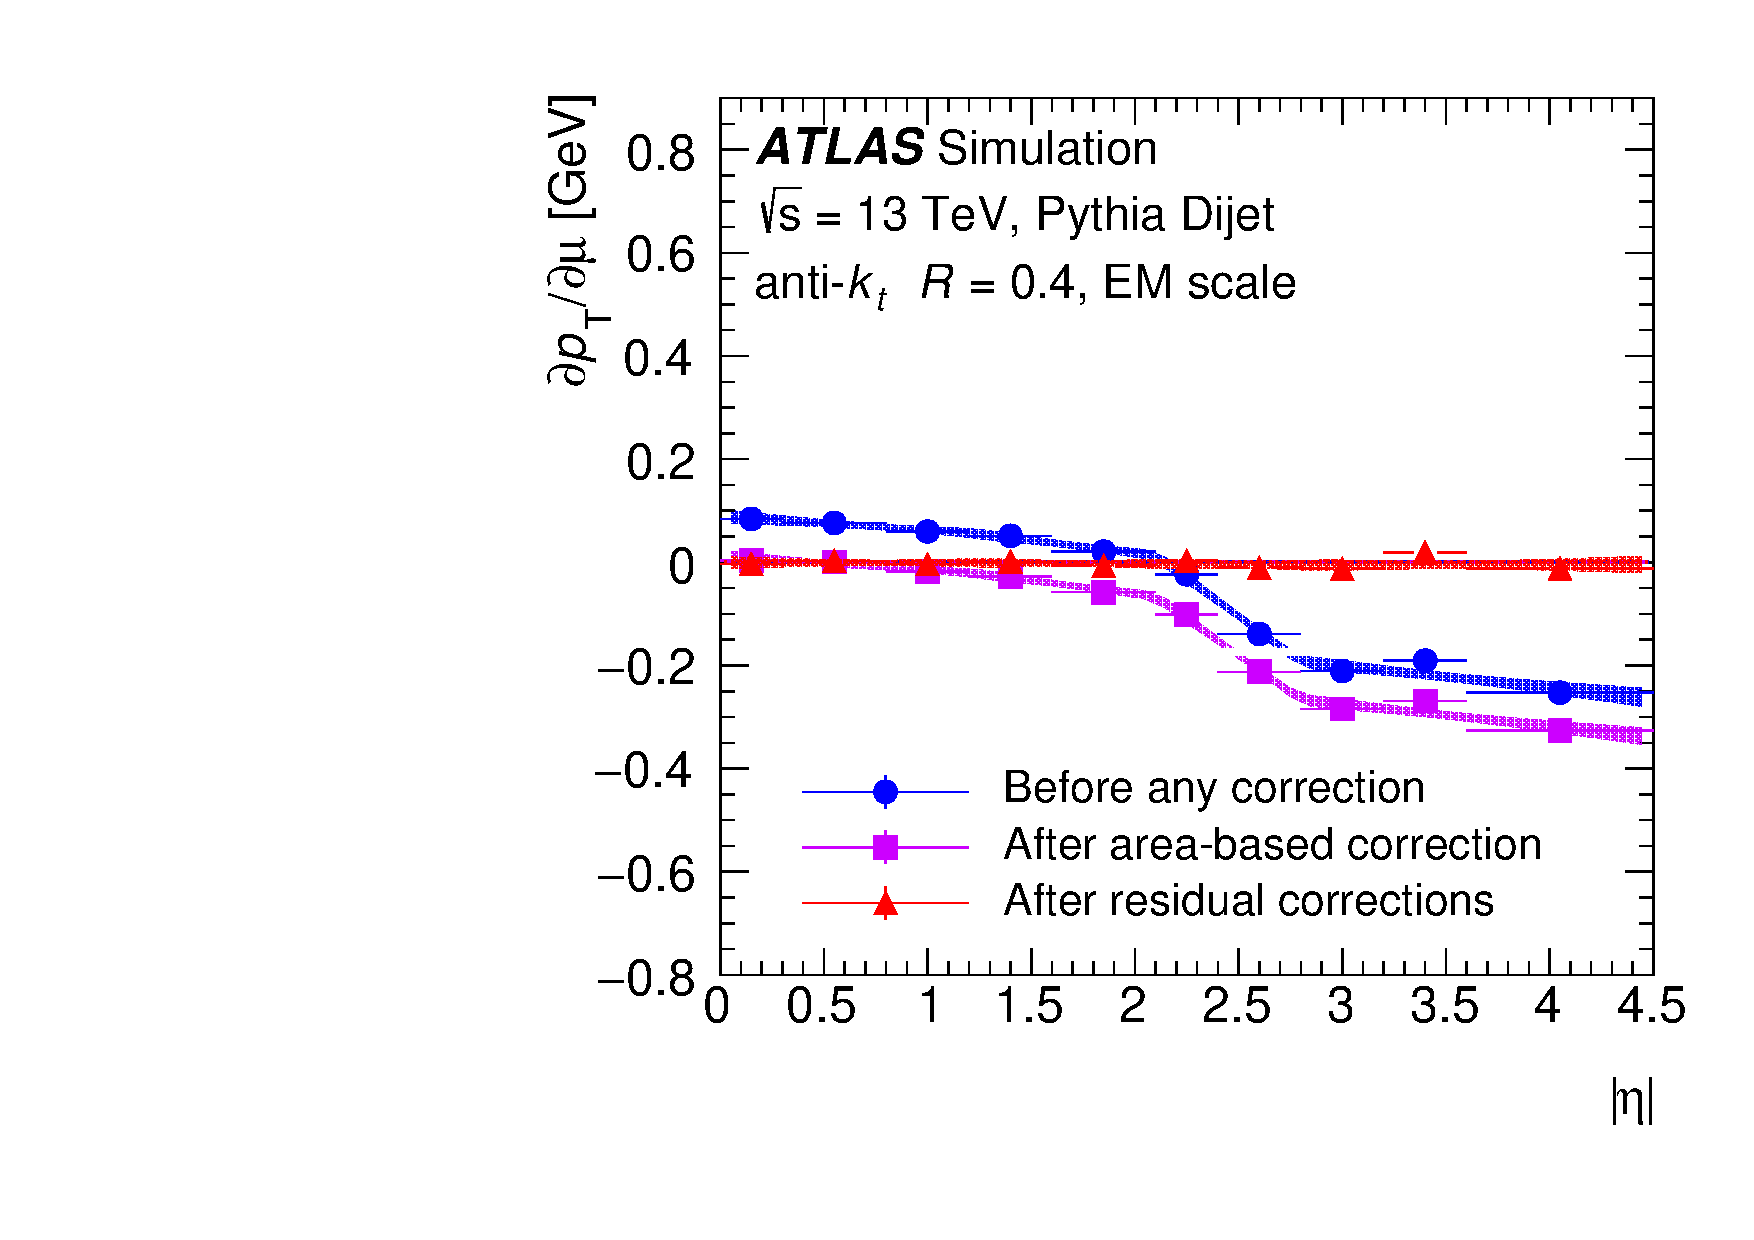
\includegraphics[width=1.\textwidth]{figures/methods/jet_pu-mu.pdf}
      \caption{Dependence of jet \pt on \(\mu\), averaged over \(N_{\text{PV}}\).}
      \label{fig:methods:event-reconstruction:jets:pileup-mu}
    \end{subfigure}
    \caption{Dependence of jet \pt on in-time pile-up (left) and out-of-time pile-up (right) as a function of \(\abs{\eta}\) for truth jet \(\pt = \SI{25}{\giga\electronvolt}\). Figures reproduced from Ref.~\cite{PERF-2016-04}.}
    \label{fig:methods:event-reconstruction:jets:smallr:pileup}
\end{figure}
\begin{enumerate}
	\setcounter{enumi}{2}
	\item \textbf{Absolute MC-based calibration}. The absolute jet energy scale (JES) and \(\eta\)-calibrations correct the reconstructed and pile-up corrected jet four momenta to the energy scale of final-state particles by accounting for non-compensating calorimeter response, energy losses in the dead material, out-of-cone effects, and biases in the jet \(\eta\)-reconstruction. Both JES and \(\eta\) calibration are parametrised in the reconstructed jet energy \(E^{\text{reco}}\) and the pseudorapidity in the detector coordinate frame \(\eta_{\text{det}}\).

	The JES calibration applies a correction, which is taken as the inverse of the average jet energy response \(\mathcal{R}\). The jet energy response \(\mathcal{R}\) is defined as the mean of a Gaussian fit to the core of the \(E^{\text{reco}} / E^{\text{truth}}\) distribution. The average jet energy response for jets with different \(E^{\text{truth}}\) as a function of \(\eta_{\text{det}}\) is shown in \Cref{fig:methods:event-reconstruction:jets:smallr:response-average}.

	The \(\eta\) calibration corrects for biases in the reconstructed jet \(\eta\), which are defined as deviations from zero in the signed difference between the reconstructed pseudorapidity \(\eta^{\text{reco}}\) and the truth pseudorapidity \(\eta^{\text{truth}}\). \Cref{fig:methods:event-reconstruction:jets:smallr:response-eta} shows the signed difference as a function of \(\eta_{\text{det}}\).

	These calibrations only change the jet \pt and \(\eta\), not the full four-momentum. Jets calibrated with the full JES and \(\eta\) calibration, are considered to be at the EM+JES scale.
\end{enumerate}
\begin{figure}[htbp]
    \centering
    \begin{subfigure}{.49\textwidth}
      \centering
      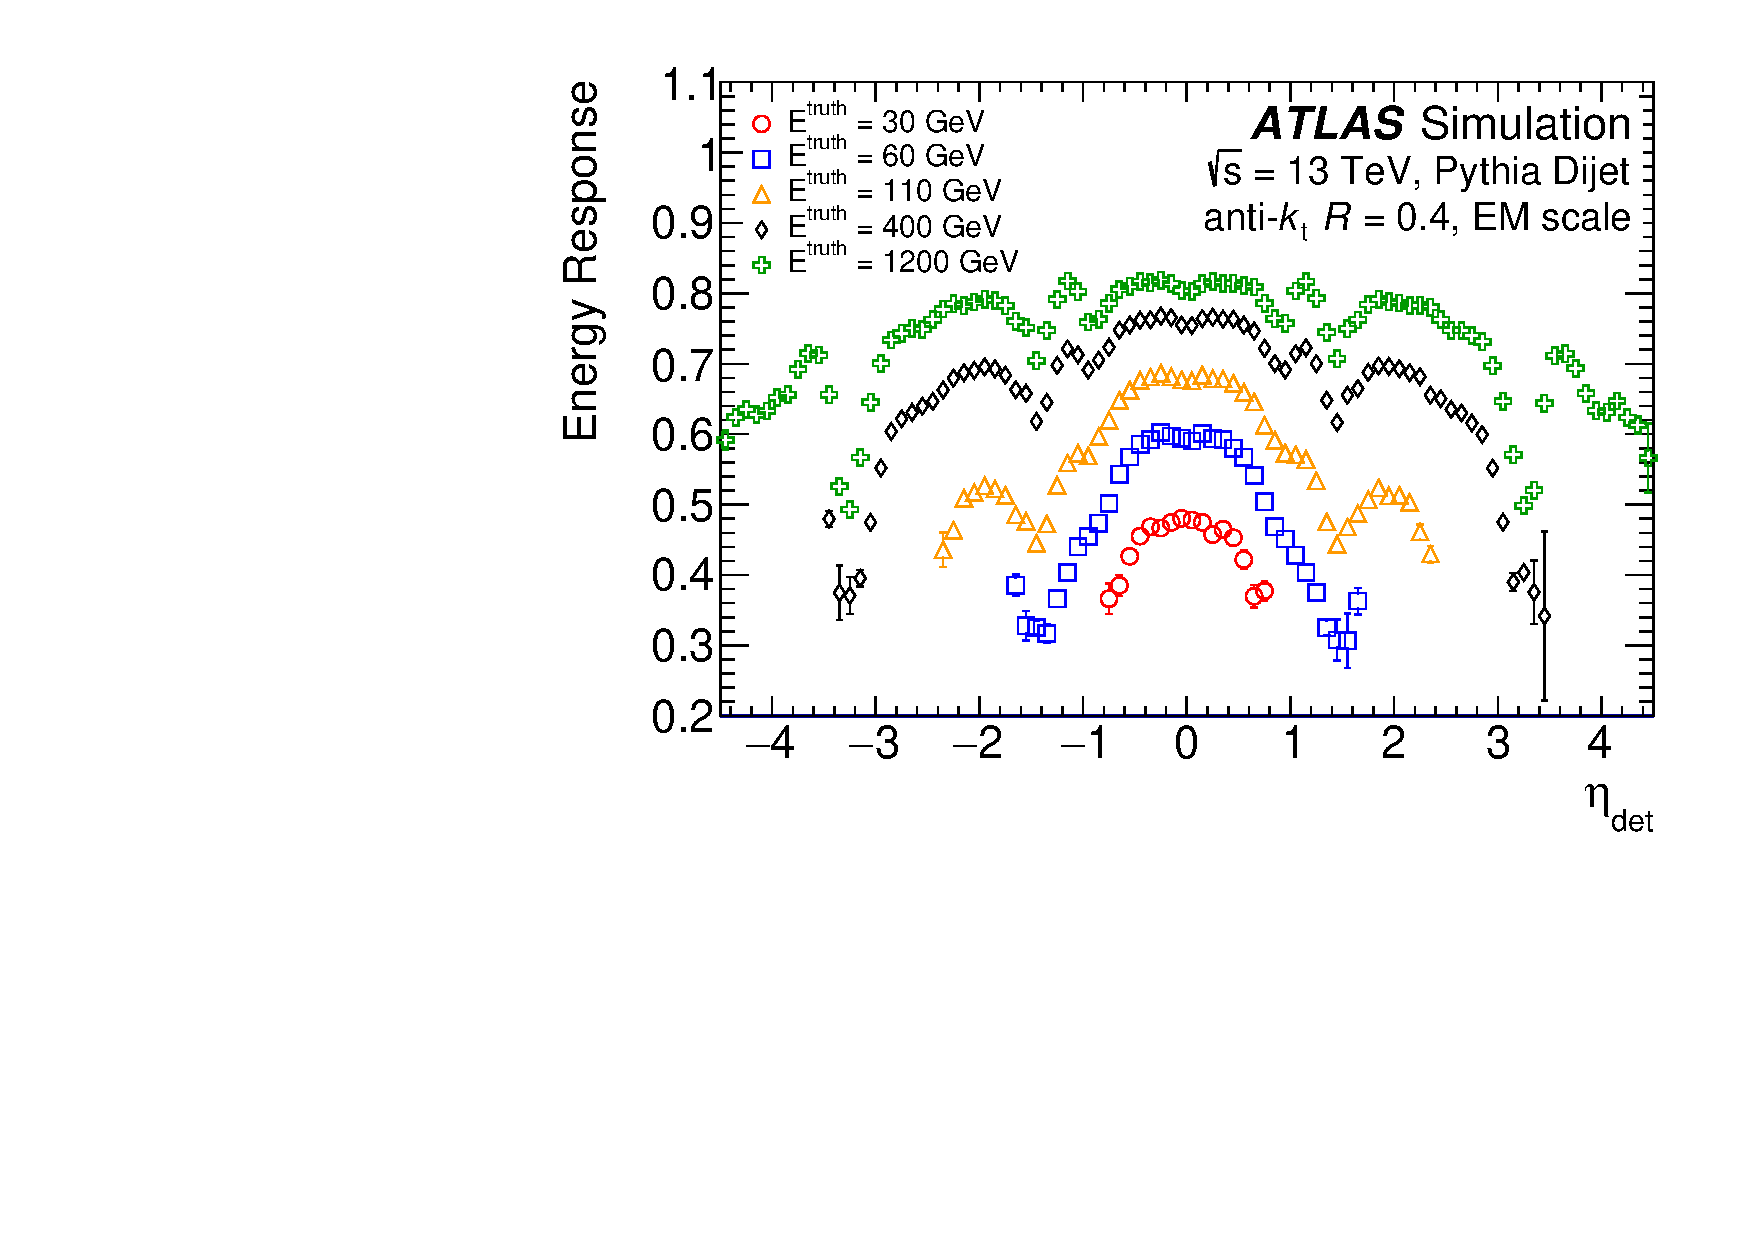
\includegraphics[width=1.\textwidth]{figures/methods/jet_response-average.pdf}
      \caption{Average jet energy response.}
      \label{fig:methods:event-reconstruction:jets:smallr:response-average}
    \end{subfigure}
    \begin{subfigure}{.49\textwidth}
      \centering
      \includegraphics[width=1.\textwidth]{figures/methods/jet_response-eta.pdf}
      \caption{Signed difference between reconstructed and truth \(\eta\) as a function of \(\eta_{\text{det}}\).}
      \label{fig:methods:event-reconstruction:jets:smallr:response-eta}
    \end{subfigure}
    \caption{The average jet energy response (left) and the signed difference between the truth and the reconstructed jet pseudorapidity (right) as functions of \(\eta_{\text{det}}\) for jets with truth energy of \num{30}, \num{60}, \num{110}, \num{400}, and \SI{1200}{\giga\electronvolt}. Figures reproduced from Ref.~\cite{PERF-2016-04}.}
    \label{fig:methods:event-reconstruction:jets:smallr:response}
\end{figure}
\begin{enumerate}
	\setcounter{enumi}{3}
	\item \textbf{Global Sequential Calibration}. The residual dependencies of jets at the EM+JES scale on features of the jet due to fluctuations in the jet particle composition and the distribution of energy within the jet are taken into account by a Global Sequential Calibration (GSC). The GSC is a series of multiplicative corrections, which are based on five jet observables, such as jet topological energy distributions or number of tracks associated with the jets. For each jet observable, an independent correction of the jet four-momentum is derived as a function jet \pt, jet energy, and \(\abs{\eta_{\text{det}}}\).

	\item \textbf{Residual in-situ calibration}. The final in-situ calibration step accounts for differences between the jet response in data and simulation by measuring the jet response in data and MC simulation separately and applying the ratio as an additional correction in data only. There are three in-situ calibrations, which are obtained from dedicated measurements involving well-calibrated reference objects. First, the jets in the forward region of the detector (\(0.8 < \abs{\eta_{\text{det}}} < 4.5\)) receive an additional correction, which brings them to the same energy scale as the jets in the central region with \( \abs{\eta_{\text{det}}} < 0.8\). Second, the jet \pt is calibrated in \HepProcess{\PZ(\Pl\Pl) + \text{jets}} and \HepProcess{\Pgamma + \text{jets}} events by balancing the hadronic recoil against a well-calibrated \PZ boson or photon. Third, single high-\pt jets are calibrated in multijet events by balancing the momentum against a system of several well-calibrated low-\pt jets. The calibration factors of the three steps are combined to a final in-situ calibration map, as shown in \Cref{fig:methods:event-reconstruction:jets:smallr:insitu}.
\end{enumerate}
\begin{figure}[htbp]
    \centering
    \includegraphics[width=.95\textwidth]{figures/methods/jet_insitu.pdf}
    \caption{Binned ratio (open circles) of the jet response in simulated events to that in data as a function of \(\eta_{\text{det}}\) for jets at the EM+JES and GSC scale with \(\SI{40}{\giga\electronvolt} < \pt^{\text{avg}} < \SI{55}{\giga\electronvolt}\). The smoothed correction (black line) with corresponding statistical (dark blue) and total (light green) uncertainty bands is overlaid, together with horizontal dotted lines to guide the eye. Figure reproduced from Ref.~\cite{PERF-2016-04}.}
    \label{fig:methods:event-reconstruction:jets:smallr:insitu}
\end{figure}

The JES calibration is accompanied by systematic uncertainties, which are defined using more than \num{90} components. As most of these uncertainties are of minor importance for most physics analyses, reduced sets of JES uncertainties are available, which combine groups of uncertainties and thereby reduce the complexity of statistical models.

In addition to the central value of the JES and the associated calibration uncertainties, the jet energy resolution (JER) needs to be determined~\cite{PERF-2014-02}. It can be parametrised by
\begin{align}
    \frac{\pt}{\sigma(\pt)} = \frac{\mathcal{N}}{\pt} \oplus \frac{\mathcal{S}}{\sqrt{\pt}} \oplus \mathcal{C},
\end{align}
where \(\mathcal{N}\) accounts for the effect of electronic and pile-up noise, \(\mathcal{S}\) denotes the stochastic term arising from the sampling nature of the calorimeters, and \(\mathcal{C}\) denotes the constant term. All terms are added in quadrature.

The JER is measured using the in-situ techniques described above, with the exception that the observable of interest is not the mean of the jet response  \(\mathcal{R}\) but its width \(\sigma(\mathcal{R})\).


\subsubsection{Identification of \bjets}
\label{sec:methods:event-reconstruction:jets:btagging}
The identification of \bjets --- jets originating from the fragmentation of \bquarks --- is an essential experimental technique to identify processes of interest even in the presence of large background contributions~\cite{ATL-PHYS-PUB-2017-013,FTAG-2018-01}.

The characteristic signature of \bjets manifests as at least one displaced decay vertex with respect to the primary vertex because of the relatively long lifetime of \PB-mesons of roughly \SI{1.5}{\pico\second}, which corresponds to a proper decay length of \SI{450}{\micro\meter}.

The identification of \bjets consists of two steps. First, various low-level algorithms process features of ID tracks and estimate their association with displaced vertices. Second, the output of these algorithms is processed by multivariate (MVA) classifiers to provide a powerful discriminant for identifying \bjets. This procedure is commonly referred to as \btagging.

The low-level \btagging algorithms include impact parameter based algorithms (IP2D and IP3D)~\cite{ATL-PHYS-PUB-2017-013}, the secondary vertex finder algorithm (SV1)~\cite{ATL-PHYS-PUB-2017-011}, and the topological multi-vertex algorithm (JetFitter)~\cite{ATL-PHYS-PUB-2018-025}. The algorithms are briefly introduced below.
\begin{itemize}
	\item The \textbf{IP2D and IP3D algorithms} are based on exploiting the large impact parameters of the tracks originating from \PB-hadron decays. While the IP2D algorithm constructs a discriminating variable using only the signed transverse impact parameter significance of tracks, the IP3D algorithm considers both the transverse and longitudinal impact parameter significances \(d_{0} / \sigma(d_{0})\) and \(\sin \theta z_{0} / \sigma(\sin \theta z_{0})\). Based on these discriminating variables and reference distributions from MC simulation, likelihood ratio discriminants are calculated for \bjet, charm jet (\cjet) and light-flavour jet identification.

	\item The \textbf{SV1 algorithm} reconstructs the single displaced vertex inside the jet which corresponds to the \PB-hadron decay using selected tracks, which have to satisfy a set of quality requirements. Likelihood ratio discriminants are constructed from vertex variables, such as the vertex mass, and the number of two-track vertices.

	\item The \textbf{JetFitter algorithm} is designed to reconstruct the full \PB-hadron decay chain, exploiting the topological features of heavy-flavour decays inside the jet. The algorithm is based on a modified Kalman filter, which is used to find a common line on which the primary, bottom and charm vertices lie, approximating the b-hadron flight path as well as the vertex positions. Likelihood ratio discriminants are constructed from the displaced vertex variables.
\end{itemize}

The commonly used high-level \btagging algorithm is the MV2 Boosted Decision Tree (BDT)~\cite{ATL-PHYS-PUB-2017-013}, which combines the outputs of the low-level \btagging algorithms with kinematic properties \pt and \(\eta\) of the jets using MVA techniques. The MV2 algorithm is trained on a mixed sample of simulated \ttbar and \PZprime events, whose background composition is adjusted to \SI{7}{\percent} \cjets and \SI{93}{\percent} light-flavour jets.

The \btagging performance is evaluated using a sample of \ttbar events. Several \btagging single-cut OPs are defined, which are based on a fixed cut on the \btagging algorithm discriminant distribution and correspond to a specific \btagging efficiency. The searches for dark matter presented in this dissertation use OPs corresponding to \SI{70}{\percent} and \SI{77}{\percent} \btagging efficiency. \Cref{fig:methods:event-reconstruction:jets:btagging:mv2} shows the distribution of the MV2 output discriminant, with the selections corresponding to \SI{70}{\percent} and \SI{77}{\percent} efficiency indicated.

\begin{figure}[htbp]
    \centering
    \includegraphics[width=.8\textwidth]{figures/methods/btagging_mv2.pdf}
    \caption{Distribution of the output discriminant of the MV2 \btagging algorithm for \bjets~(blue), \cjets~(green) and light-flavour jets~(red) in a sample of MC simulated \ttbar events. Figure adapted from Ref.~\cite{FTAG-2018-01}.}
    \label{fig:methods:event-reconstruction:jets:btagging:mv2}
\end{figure}

The corresponding rejection factors for \cjets and light-flavour jets at the \SI{77}{\percent} (\SI{70}{\percent}) fixed-cut efficiency selection are approximately \num{5} and \num{110} (\num{9} and \num{300}), respectively.

The \btagging efficiency, as well as the misidentification rates of \cjets and light-flavour jets, are compared between data and simulations. Corrections in the form of scale factors are applied to simulated events to account for discrepancies between data and simulations due to imperfections in the modelling of physics processes or the detector response.

\Cref{fig:methods:event-reconstruction:jets:btagging:corrections} shows the measured \btagging efficiency in dependence of the jet \pt and the scale factors, which are applied to simulated events. The scale factors have values close to unity and are approximately constant throughout the entire \pt range.

\begin{figure}[htbp]
    \centering
    \begin{subfigure}{.49\textwidth}
      \centering
      \includegraphics[width=1.\textwidth]{figures/methods/btagging_efficiency70.pdf}
      \caption{\btagging efficiency}
      \label{fig:methods:event-reconstruction:jets:btagging:corrections:efficiency}
    \end{subfigure}
    \begin{subfigure}{.49\textwidth}
      \centering
      \includegraphics[width=1.\textwidth]{figures/methods/btagging_sf70.pdf}
      \caption{\btagging efficiency simulation-to-data scale factors}
      \label{fig:methods:event-reconstruction:jets:btagging:corrections:sf}
    \end{subfigure}
    \caption{The \btagging efficiency (left) and \btagging efficiency simulation-to-data scale factors (right) for the \SI{70}{\percent} single-cut OP of the MV2 tagger as a function of jet \pt. The efficiency measurement is shown in data (dots) and in simulated \ttbar events (red line), together with the total uncertainty (green band). Figures reproduced from Ref.~\cite{FTAG-2018-01}.}
    \label{fig:methods:event-reconstruction:jets:btagging:corrections}
\end{figure}

\subsubsection{Large-radius calorimeter jets}
\label{sec:methods:event-reconstruction:jets:larger}
The reconstruction of hadronically decaying heavy bosons using a pair of small-radius jets becomes infeasible for boosted objects. The strong collimation of their decay products as a consequence of the Lorentz boost makes it impossible to resolve the decay's partonic sub-structure. As a rule-of-thumb, the separation between the two decay products of a boosted heavy boson with mass \(m\) and transverse momentum \pt can be estimated~\cite{Butterworth2008} as
\begin{align}
    R = \frac{1}{z (1-z)} \times \frac{m}{\pt},
\end{align}
where \(z\), \(1-z\) are the momentum fractions of the two decay products.
As heavy bosons have a larger transverse momentum, their decay products become increasingly collimated, as illustrated in \Cref{fig:methods:event-reconstruction:jets:larger:boosted}.
Therefore, the reconstruction of the boosted object is based on a single jet with large radius parameter, which can fully contain the boosted heavy boson decay.

\begin{figure}[htbp]
    \centering
    \includegraphics[width=.95\textwidth]{figures/methods/jet_boosted.pdf}
    \caption{Illustration of boosted event topologies: the distance between the decay products of a boosted boson decreases with increasing transverse momentum of the boosted boson.}
    \label{fig:methods:event-reconstruction:jets:larger:boosted}
\end{figure}

The reconstruction and calibration procedure of large-radius jets consists of several stages, which are illustrated by \Cref{fig:methods:event-reconstruction:jets:larger:calibration}.

\begin{figure}[htbp]
	\centering
	\includegraphics[width=0.95\textwidth]{figures/methods/jet_larger_calibration.pdf}
	\caption{Overview of the large-radius jet reconstruction and calibration procedure. Illustration reproduced from Ref.~\cite{JETM-2018-02}.}
	\label{fig:methods:event-reconstruction:jets:larger:calibration}
\end{figure}

Large-radius jets are reconstructed from topological clusters in the calorimeters, which are calibrated to the hadronic scale in the LCW scheme, using the \antikt algorithm with a radius parameter \(R = 1.0\).

The large radius parameter makes the reconstructed jets particularly susceptible to contamination from pile-up, initial-state radiation, and multiple parton interactions. The contributions of these processes are generally softer  than those of the hard scattering process and can therefore be suppressed by jet grooming algorithms~\cite{Kogler2019}.
Among the large variety of algorithms which has been studied~\cite{Dasgupta2013,Ellis2010,Larkoski2014,Dreyer2018}, the commonly adapted jet trimming algorithm~\cite{Krohn2010} is used to remove soft contaminations of the large-radius jets. All particles in a large-radius jet with radius \(R\) are re-clustered into sub-jets with radius parameter \(R_{\text{sub}} < R\) using the \(k_{\text{T}}\)-algorithm. The resulting sub-jets that satisfy the condition \(\pt^{\text{sub-jet}} > f_{\text{cut}} \pt^{\text{large-radius jet}}\) are kept and merged to form the trimmed large-radius jet. The algorithm is illustrated in \Cref{fig:methods:event-reconstruction:jets:larger:trimming}.

\begin{figure}[htbp]
	\centering
	\includegraphics[width=0.95\textwidth]{figures/methods/jet_trimming.pdf}
	\caption{Illustration of the jet-trimming algorithm for large-radius jets. Figure reproduced from Ref.~\cite{PERF-2012-02}.}
	\label{fig:methods:event-reconstruction:jets:larger:trimming}
\end{figure}

The trimmed large-radius jets are calibrated to the energy scale of final-state particles using corrections derived in MC simulations. These simulations correct the \pt, \(\eta\), and the jet mass.
Finally, the jets undergo a residual in-situ calibration using jet response measurements in \HepProcess{\Pp\Pp} collision data. Similar to the small-radius jets, the correction is derived from a statistical combination of data-to-simulation ratios of these response measurements and is applied only to data.

The large-radius jet mass resolution is improved by using both calorimeter and tracking information in the reconstruction.
The calorimeter-based (CA) jet mass is computed from the energies \(E_{i}^{\text{topo}}\) and momenta \(\vec{p}_{i}^{\text{topo}}\) of topological clusters in the calorimeter as
\begin{align}
    m^{\text{CA}} = \sqrt{\left(\sum_{i} E_{i}^{\text{topo}}\right)^2 - \left(\sum_{i} \vec{p}_{i}^{\text{topo}}\right)^2}.
\end{align}

The track-assisted (TA) mass is computed in a similar way from a mass measurement based on ID tracks \(m^{\text{track}}\) but additionally weighted with the ratio of the transverse momenta measured by the calorimeters (\(\pt^{\text{calo}}\)) and the ID (\(\pt^{\text{track}}\)) to account for neutral hadrons. It is defined as
\begin{align}
    m^{\text{TA}} = m^{\text{track}} \times \frac{\pt^{\text{calo}}}{\pt^{\text{track}}}.
\end{align}

The combined jet mass is defined as the weighted least-squares combination of the CA and TA mass definitions
\begin{align}
    m^{\text{comb}} = \frac{\sigma_{\text{CA}}^{-2}}{\sigma_{\text{CA}}^{-2} + \sigma_{\text{TA}}^{-2}} \times m^{\text{CA}} + \frac{\sigma_{\text{TA}}^{-2}}{\sigma_{\text{CA}}^{-2} + \sigma_{\text{TA}}^{-2}} \times m^{\text{TA}},
\end{align}
with the respective mass resolutions \(\sigma_{\text{CA}}\) and \(\sigma_{\text{TA}}\).

The combined jet mass definition improves the jet mass resolution and reduces the systematic uncertainties, as shown in \Cref{fig:methods:event-reconstruction:jets:larger:combinedmass}.

\begin{figure}[htbp]
  \centering
  \includegraphics[width=0.75\textwidth]{figures/methods/combinedmass.pdf}
  \caption{The fractional jet mass resolution, defined as half the ratio of the \SI{68}{\percent} confidence interval inter-quantile range of the jet mass response distribution and the median jet response, estimated in dependence of the truth jet \pt using simulated hadronic decays of diboson processes. Figure reproduced from Ref.~\cite{JETM-2017-002}.}
  \label{fig:methods:event-reconstruction:jets:larger:combinedmass}
\end{figure}


\subsubsection{Track jets}
\label{sec:methods:event-reconstruction:jets:trackjets}
The track jets supplement the reconstruction of boosted heavy bosons based on large-radius jets by enabling the identification of the large-radius jet's flavour content.

Track jets with fixed radius parameter are reconstructed using the \antikt algorithm with \(R=0.2\) on ID tracks originating from the PV with \(\pt >  \SI{0.5}{\giga\electronvolt}\) and \(\abs{\eta} < 2.5\). The tracks are required to have at least seven hits in total in the SCT and PXD detectors, no more than one hit shared by multiple tracks in the PXD detector, and at most one missing hit in the PXD or two missing hits in the SCT detectors.
An additional requirement on the longitudinal impact parameter \(\abs{z_0 \sin \theta} < \SI{3}{\milli\meter}\) with respect to the PV reduces the pile-up contribution.

The smaller radius parameter and superior angular resolution of the tracking detector allow resolving the partonic substructure of the heavy boson decay even in dense environments.
However, for substantially boosted event topologies, even the track jets can overlap if they are reconstructed with a fixed radius parameter. The problem of track jet merging is overcome by the use of a modified jet algorithm in which the radius parameter decreases with increasing jet transverse momentum as the jet is being formed. The scaling of the effective jet radius
\begin{align}
R_{\text{eff}} = \frac{\rho}{\pt},
\end{align}
with the transverse momentum of the pseudo-jet \pt as it is being formed (c.f. \Cref{sec:pp:jets}) is determined by the parameter \(\rho = \SI{30}{\giga\electronvolt}\). The effective jet radius is bounded by \(0.02 \leq R_{\text{eff}} \leq  0.4\). The resulting jets are referred to as variable-radius (VR) track jets~\cite{Krohn2009,ATL-PHYS-PUB-2017-010}. The reconstruction of VR track jets in comparison to that of FR track jets with radius parameter \(R=0.2\) is illustrated in \Cref{fig:methods:event-reconstruction:jets:trackjets:illustration}.

\begin{figure}[hbtp]
  \centering
  \includegraphics[width=0.65\textwidth]{figures/methods/vrtrackjets_cartoon.pdf}
  \caption{Illustration of the sub-jet reconstruction using either fixed radius (left) or variable radius (right) track jets. Figure reproduced from Ref.~\cite{ATL-PHYS-PUB-2017-010}.}
  \label{fig:methods:event-reconstruction:jets:trackjets:illustration}
\end{figure}

The track jets are uniquely associated with a large-radius jet using the ghost-association technique, in which ghost particles --- copies of the track jet four-momentum with vanishing momentum --- are added to the inputs of the large-radius jet algorithm. This procedure allows for the unique association of the track jets with a large-radius jet by identifying the ghost particles associated with the non-trimmed large-radius jet.

Track jets undergo no calibration procedure, as the kinematic properties of the heavy boson are reconstructed from large-radius jet information and the track jets are only used for the identification of the large-radius jet flavour.
Similar to small-radius jets, the MV2 \btagging algorithm is used to identify track jets originating from \bquarks.
The \btagging efficiency and the misidentification rates for \cjets and light-flavour jets are compared between data and MC to derive corrections for simulated events.


\subsection{Tau leptons}
\label{sec:methods:event-reconstruction:taus}
As \Pgt leptons have a proper decay length of \(c\tau = \SI{87}{\micro\meter}\)~\cite{Tanabashi2018} and subsequently decay within the LHC beam pipe, their leptonic decays are reconstructed as stable electrons or muons.

The hadronically decaying \Pgt leptons are reconstructed as small-radius jets and identified using MVA techniques, conceptually similar to \btagging.
\Pgt decays exhibit a characteristic signature of either 1 or 3 charged hadrons collimated along the jet axis accompanied by neutral hadrons. A combination of boosted decision trees targets the 1-prong and 3-prong \Pgt decay modes and allows for the definition of working points with increasing purity and decreasing efficiency, including the \textsc{Loose} BDT OP which is used in the dark matter searches presented in this dissertation.

\subsection{Missing transverse momentum}
\label{sec:methods:event-reconstruction:met}
The missing transverse momentum \met is a key observable when searching for undetected objects such as dark matter particles or neutrinos. The almost hermetic design of the ATLAS detector enables the reconstruction of these objects via the transverse momentum balance in a collision event. The composite nature of the protons undergoing the collision restricts the knowledge of the momentum before the collision to the transverse plane, where it is zero since the full momentum is aligned in the beam direction. Thus, any momentum imbalance in the transverse plane after the collision can be attributed to undetected objects.

The missing transverse momentum is defined as the negative sum of all physics object transverse momentum vectors and a component due to the track soft term (TST)
\begin{align}
\met = - \left| \sum_{e, \mu, \gamma, \tau, \text{jets}} \vec{p}_{\text{T}} \, + \sum_{\text{soft term}} \vec{p}_{\text{T}} \right|.
\end{align}
A high reconstruction efficiency for objects entering the \met computation is desirable, therefore loose object definitions are employed when calculating the missing transverse momentum.
The TST  is composed of all tracks not associated with physics objects and is particularly relevant for estimating the \met scale and resolution.

As \met is of paramount importance not only for dark matter searches, several OPs are defined for the competing needs of various analyses in terms of pile-up suppression and \met resolution.
\begin{itemize}
	\item \textsc{Loose}. The \met calculation includes jets with \(\pt > \SI{20}{\giga\electronvolt}\) and \(\abs{\eta} < 4.5\). Jets with \(\pt < \SI{60}{\giga\electronvolt}\) and \(\abs{\eta} < 2.4\) are required to pass the Jet Vertex Tagger (JVT) selection with a JVT score of \(\text{JVT} >  0.59\).
	\item \textsc{Tight}. The \met calculation includes the jets described in the \textsc{Loose} OP definition. In addition, forward jets (\(2.4 < \abs{\eta} < 4.5\) must satisfy \(\pt > \SI{30}{\giga\electronvolt}\).
\end{itemize}
The \textsc{Tight} OP offers better pile-up suppression at the cost of inferior \met resolution for low pile-up events with respect to the \textsc{Loose} OP.
\Cref{fig:methods:event-reconstruction:met:resolution} shows the \met resolution in dependence of the number of primary vertices \(N_{\textsc{PV}}\) in the event for the two OPs.

\begin{figure}[hbtp]
  \centering
  \includegraphics[width=0.7\textwidth]{figures/methods/met_resolution.pdf}
  \caption{Distribution of the \met resolution in dependence of the number of primary vertices \(N_{\textsc{PV}}\) in the event for \met reconstructed with the \textsc{Loose} and \textsc{Tight} operating points in \HepProcess{\PZ \to \Pgm\Pgm} events. Figure adapted from Ref.~\cite{ATLAS-CONF-2018-023}.}
  \label{fig:methods:event-reconstruction:met:resolution}
\end{figure}

A related variable \mpt is defined as the negative vectorial sum of the transverse momenta of all tracks associated with the primary vertex. This variable is used to reduce beam-induced and non-collision backgrounds.

The \textbf{missing transverse momentum significance} is used to separate events in which the reconstructed missing transverse momentum \met is genuinely coming from dark matter particles or neutrinos from events with fake \met being observed due to contributions from particle-measurement or resolution effects.
In addition to historical definitions of the \met significance, where the scalar sum of objects entering the \met calculation \(\sum \met\) serves as an event-based approximation to the full \met resolution, an object-based \met significance definition is considered.

The object-based \met significance \(\mathcal{S}\)~\cite{ATLAS-CONF-2018-038} takes into account the resolutions and full correlation among all objects entering the \met reconstruction.
In a coordinate system, which is rotated parallel (longitudinal L) and perpendicular (transverse T) to the direction of the missing transverse momentum vector, the object-based \met significance definition can be written as
\begin{align}
    \mathcal{S}^2 & = %
	    \begin{pmatrix} \met & 0 \end{pmatrix} %
	    \begin{pmatrix} \sigma_{L}^{2} & \rho_{LT} \sigma_{L} \sigma_{T} \\ \rho_{LT} \sigma_{L} \sigma_{T} & \sigma_{T}^{2} \end{pmatrix}^{-1} %
	    \begin{pmatrix} \met \\ 0 \end{pmatrix} \\ %
               & = \frac{\left(\met\right)^2}{\sigma_{L}^{2}\left(1-\rho_{LT}^{2}\right)},
\end{align}
where \(\sigma_{L}^{2}\) and \(\sigma_{T}^{2}\) are the total variances in the longitudinal (L) and transverse (T) directions to the \(\vec{\met}\) vector, respectively, and \(\rho_{LT}\) is the correlation factor of the two measurements. These variances consider all fluctuations in the direction (L) or perpendicular (T) to the direction of the reconstructed \met from the hard objects entering the \met calculation.

A high value of \(\mathcal{S}\) is an indication that the observed \met in the event cannot be accounted for by resolution smearing alone, suggesting that the event may contain unseen objects such as neutrinos or dark matter particles.

\Cref{fig:methods:event-reconstruction:metsignificance:performance} illustrates the performance of the object-based \met significance in comparison to an event-based definition of \met significance and \met itself. The object-based \met significance definition is clearly superior, as it provides rejection of over \SI{98}{\percent} of the background processes with fake \met while retaining a signal efficiency over \SI{80}{\percent}. In comparison, \met and the event-based \met significance provide background rejection of \SI{55}{\percent} and \SI{75}{\percent}, respectively~\cite{ATLAS-CONF-2018-038}.

\begin{figure}[htbp]
	\centering
	\includegraphics[width=0.75\textwidth]{figures/methods/met_significance.pdf}
	\caption{Performance of the \met significance in terms of background rejection versus signal efficiency in simulated \HepProcess{\PZ \to \Pe \Pe} and \HepProcess{\PZ \to \Pe \Pe \Pgn \Pgn} samples with a \HepProcess{\PZ to \Pe \Pe} selection. The performance is shown for \met~(orange), event-based \met significance~(pink), and object-based \met significance~(green) as discriminants in events with a \(\met > \SI{100}{\giga\electronvolt}\) pre-selection. The lower panel shows the ratio of other definitions to the event-based \met significance. Figure reproduced from Ref.~\cite{ATLAS-CONF-2018-038}.}
	\label{fig:methods:event-reconstruction:metsignificance:performance}
\end{figure}

\newpage

\section{Statistical methods}
\label{sec:methods:statistics}
Common statistical methods used in all searches for dark matter presented in this dissertation are introduced in this section.

The simplest definition of a fit is based on a statistical model only considering the total number of selected events. Typically, the statistical model is based on simulated samples of the signal (\(S\)) and background (\(B\)) processes, which provide the predicted event yields for the respective processes.
A maximum-likelihood fit of the model to data determines the best-fit values of the parameter of interest (POI) and the nuisance parameters (NP) \(\vec{\theta}\). The POI is typically taken to be the signal strength \(\mu\), which is defined as the ratio of the signal cross section to a reference signal cross section predicted by theory. The NPs denote further parameters in the model which are subject to uncertainties, e.g. the individual background normalisation parameters.
The total predicted event yield is
\begin{align}
    N^{\text{exp}} (\mu, \vec{\theta}) = \mu S(\vec{\theta}) + B(\vec{\theta}).
\end{align}
The sensitivity to signal processes can be enhanced by considering not only the total event yield but distributions of discriminating variables. These variables are chosen to provide strong separation between signal and background processes. The statistical model for such a fit based on binned distributions of the discriminating variables is described by the likelihood function
\begin{align}
	\mathcal{L}(N^{\text{obs}} | \mu, \vec{\theta}) = %
	\text{Pois}(N^{\text{obs}} | N^{\text{exp}} (\mu, \vec{\theta})) %
	\times \left[ %
		\prod_{i \in \text{bins}} \frac{\mu S_i(\vec{\theta}) + B_i(\vec{\theta})}{N^{\text{exp}} (\mu, \vec{\theta})}
	\right] %
	\times \prod_{\theta_{i} \in \vec{\theta}} f(0 | \theta_{i}),
	\label{eq:methods:statistics:likelihood}
\end{align}
where \(N^{\text{obs}}\) denotes the total observed event yield and \(S_{i}\), \(B_{i}\) denote the number of predicted signal and background events in bin \(i\), respectively.
The systematic uncertainties are implemented as the NPs \(\theta_{i}\) with the associated probability density functions \(f(0|\theta_{i})\).
These are parametrised as standard Gaussian prior distributions with the expectation value \(\theta_{i}\), or in the case of normalisation uncertainties as Log-normal distributions to ensure a positive value of the likelihood function.

A common technique to reduce the uncertainties on the background modelling is the use of control region data.
Auxiliary measurements in dedicated selections which are enriched in the respective background processes provide constraints on the normalisation of the simulated backgrounds.

The searches presented in this dissertation use a profile likelihood fit which is based on \Cref{eq:methods:statistics:likelihood} and is implemented using the \textsc{HistFactory}~\cite{Cranmer2012} software.
The results are obtained by maximising the likelihood function \(\mathcal{L}(N^{\text{obs}} | \mu, \theta)\) under consideration of the likelihood ratio test statistic \(q_{\mu}\). The latter is the most powerful test statistic one can construct~\cite{Neyman1933} and is defined by
\begin{align}
    q_{\mu} = - 2 \ln{\left(\frac{\mathcal{L}(\mu, \doublehat{\vec{\theta}})}{\mathcal{L}(\hat{\mu}, \hat{\vec{\theta}})}\right)},
\end{align}
where \(\mathcal{L}(\mu, \doublehat{\vec{\theta}})\) is maximised over all NPs for a given value of \(\mu\) and \(\mathcal{L}(\hat{\mu}, \hat{\vec{\theta}})\) denotes the global maximum of the full parameter space \(\mu, \vec{\theta}\). Here, \(\doublehat{\vec{\theta}}\) is referred to as the conditional maximum-likelihood estimator of \(\vec{\theta}\), whereas \(\hat{\mu}\) and \(\hat{\vec{\theta}}\) are referred to as the unconditional maximum-likelihood estimators of \(\mu\) and \(\vec{\theta}\), respectively.

The test statistic \(q_{\mu}\) can be used to test a given signal strength \(\mu\) hypothesis.
Searches for new physics processes, which manifest as a significant excess over the SM background, consider the ``background-only'' hypothesis with \(\mu=0\) as the null hypothesis. The test for discovery is performed by rejecting the null hypothesis using the test statistic
\begin{align}
    q_{0} = \begin{cases} - 2 \ln \left(\frac{\mathcal{L}(0, \doublehat{\vec{\theta}})}{\mathcal{L}(\hat{\mu}, \hat{\vec{\theta}})}\right) & \text{for } \hat{\mu} > 0 \\ 0 & \text{for } \hat{\mu} \leq 0. \end{cases}
\end{align}
Large values of \(q_{0}\) correspond to more observed events than could be explained by ``background-only'' hypothesis, suggesting the presence of a signal.

Typically, tests for discovery are stated in terms of the significance
\begin{align}
Z_{\mu} = 1 - \Phi^{-1}(1 - p_{\mu}),
\end{align}
which is defined by the inverse of the cumulative distribution of the standard Gaussian \(\Phi^{-1}\).

If no excess is found in these searches, constraints on the parameter space of specific models for the new physics processes can be set using a different hypothesis test. The test for exclusion is performed by rejecting the ``signal + background'' hypothesis, using the test statistic
\begin{align}
q_{\mu} = \begin{cases} -2 \ln{\left(\frac{\mathcal{L}(\mu, \doublehat{\vec{\theta}})}{\mathcal{L}(0, \hat{\vec{\theta}})}\right)} & \text{for } \hat{\mu} \leq 0 \\ -2 \ln{\left(\frac{\mathcal{L}(\mu, \doublehat{\vec{\theta}})}{\mathcal{L}(\hat{\mu}, \hat{\vec{\theta}})}\right)} & \text{for } 0 < \hat{\mu} \leq \mu \\ 0 & \text{for } \hat{\mu} > \mu.  \end{cases}
\end{align}
Here, the additional condition for \(\hat{\mu}\) avoids considering an excess in data incompatible with the ``signal + background'' hypothesis.
Large values of \(q_{\mu}\) indicate smaller compatibility of the ``signal + background'' hypothesis and the observed data.
The fact that the test-statistic is defined to be non-zero only for \(\hat{\mu} \leq \mu\) implies that only upper limits on \(\mu\) are considered.

The result of the hypothesis test is described by the \(p\)-value
\begin{align}
    p_{\mu} = \int_{q_{\mu}^{\text{obs}}} f(q_{\mu} | \mu) \dd{q_{\mu}},
\end{align}
which quantifies the level of disagreement between the observed data and the statistical model defined by the probability density function \(f(q_{\mu | \mu})\) of \(q_{\mu}\) for a signal strength \(\mu\).

Corresponding \(p\)-values for the ``background-only'' (\(b\)) and the ``signal + background'' (\(s+b\)) hypotheses for a given \(q_{\mu}^{\text{obs}}\) are defined by
\begin{align}
    p_{b} &= \int_{-\infty}^{q_{\mu}^{\text{obs}}} f(q_{\mu} | b) \dd{q_{\mu}} \\
    p_{s+b} &= \int_{q_{\mu}^{\text{obs}}}^{\infty} f(q_{\mu} | s + b) \dd{q_{\mu}}.
\end{align}

These definitions, however, might lead to accidental exclusion of signals for searches which are insensitive to those signals. This might occur if, for instance, there is a downward fluctuation in data relative to the expectation of the background-only hypothesis.
The accidental rejection of signal hypotheses can be avoided by using the \(\text{CL}_{s}\) method~\cite{Read:2002hq}, in which the \(p_{s+b}\) value is weighted by a penalty factor that increases with decreasing sensitivity. The \(\text{CL}_{s}\) value is defined by
\begin{align}
    \text{CL}_{s} = \frac{p_{s+b}}{1 - p_{b}}.
\end{align}
Adopting the \(\text{CL}_{s}\) definition, a point in the parameter space of a model is excluded with confidence level \(1 - \alpha\) if one finds \(\text{CL}_{s} < \alpha\). Evidently, the \(\text{CL}_{s}\) is more conservative, as the \(\text{CL}_{s}\)-based exclusion criterion is more stringent than the usual requirement \(p_{\mu} < \alpha\).
However, it should be pointed out that \(\text{CL}_{s}\) limits have no well-defined coverage and should be interpreted such that the probability of having falsely excluded a signal is less than \(\alpha\).

The observed value of the test statistic \(q_{\mu}^{\text{obs}}\) will differ in independent experiments, as it is subject to statistical fluctuations. When computing the expectation value of \(q_{\mu}\), the underlying probability distribution of the test statistic can in general not be evaluated analytically. It can, however, be approximated.
The approximation can be based on evaluating a large number of simulated toy experiments. Although, in principle, these replicas enable the determination of the expectation value of \(q_{\mu}\) with arbitrarily high precision, it comes at the price of high computational cost.

The Asimov method~\cite{Cowan:2010js,Cowan:2010js-err} is an alternative approach which is based on an artificially constructed, representative dataset. The use of the Asimov dataset is formally justified in the limit of large numbers, in which \(\hat{\mu}\) follows a Gaussian distribution.
It can be used to validate the statistical model and to estimate various properties, such as the expected \(p\)-values, exclusion limits, or the impact of different sources of uncertainty.
The expected median discovery significance is estimated with Asimov data generated under the assumption of the nominal signal model (\(\mu=1\)). Conversely, the expected exclusion limits are estimated with Asimov data generated under the assumption of the background-only hypothesis (\(\mu=0\)).


\section{RECAST}
\label{sec:methods:recast}
The searches for new physics phenomena beyond the SM represent a significant investment in time and both human and computational resources. Moreover, as there are plenty of models predicting new phenomena, it becomes increasingly difficult to experimentally test all of them with dedicated searches considering only specific models in their interpretation.
Given the steadily growing number of potentially interesting models and seeing the dawn of the high-luminosity era, a powerful reinterpretation framework is urgently needed.
Existing searches for new phenomena often are sensitive to a larger class of new physics theory models. Therefore, it is the sustainable approach to reinterpret existing searches instead of designing a new one.

The RECAST framework~\cite{Cranmer2011} is designed to reuse estimates of backgrounds, systematic uncertainties, and observed data from preserved searches to test alternative signal hypotheses.
A faithful reinterpretation entails processing the MC generated samples associated with the alternative signals using the full analysis workflow, including the algorithmic implementation of object reconstruction, event selection, and statistical evaluation.
RECAST provides the computational infrastructure of preserving the analysis software and automating the corresponding workflow to organise systematic reinterpretation of analyses efficiently.

The analysis software is preserved in a manner that is portable and compatible with an extensive range of computing infrastructures. This is achieved by building Docker container images~\cite{Containers2014, Docker2014}, which can be thought of as a snapshot of a file-system containing the analysis software with all its dependencies.
The preservation of the workflow is achieved through the use of the \textsc{yadage}~\cite{Cranmer2017} workflow description language.
The workflow is modelled as a directed acyclic graph, consisting of several interdependent processing steps (referred to as jobs), which culminate in the statistical inference. Within \textsc{yadage}, the workflow structure and the job templates are captured as YAML documents. The parametrised job templates specify the commands which configure and execute the analysis software, while the workflow orchestrates the individual steps.

Capturing both the software and the workflow allows for re-executing the analysis software chain without expert knowledge, which otherwise might get lost if the original authors leave the collaboration.
A growing number of ATLAS searches is archived using RECAST, thereby providing faithful reinterpretations even for searches with involved analysis techniques~\cite{ATL-PHYS-PUB-2020-007}, which cannot be captured by simplified third-party implementations.


% \part{Studies of the ATLAS muon trigger}
% % !TEX root = ../my-thesis.tex
%
\chapter{Improvements to the ATLAS muon trigger}
\label{sec:trigger}

\section{Introduction}
\label{sec:trigger:introduction}
Searches for new physics phenomena motivated by the presence of dark matter in the universe rely on the accurate description of electroweak background processes. The wealth of data collected at the LHC with the ATLAS experiment improves the understanding of these background processes. A large range of LHC physics measurements depends crucially on the reliable identification and efficient reconstruction of leptons with momenta at the electroweak scale.

The ATLAS muon trigger constitutes the first stage of the muon detection and reconstruction. It selects events containing muons with their momentum above specified thresholds out of the extremely high background. Improvements to the trigger systems directly impact all physics measurements, as the trigger decision irreversibly determines which data is recorded. The trigger performance is quantified by the muon efficiency and the trigger rate. The muon efficiency is the fraction of events accepted by the trigger, which contain muons above a certain transverse momentum threshold. The trigger rate is the total rate of recorded events. Good muon trigger performance is characterised by high muon efficiency and a low fraction of fake or low-\pt muons in the trigger rate.

This section presents a study about the potential reduction of the trigger rate of the muon trigger with the lowest \pt threshold of \SI{4}{\giga\electronvolt} (L1MU4) by careful tuning of the trigger logic.

\section{Rate reduction of the L1MU4 trigger}
\label{ssec:trigger:l1mu4}
\subsection{The ATLAS L1 muon trigger in Run-2}
\label{ssec:trigger:l1mu4:run2}
The first stage of the ATLAS muon trigger (L1 muon trigger) performs an initial selection of collision events containing muons with transverse momentum above certain thresholds. The trigger decision is based on a subset of detectors with reduced granularity but excellent timing resolution, which allows associating the events with individual bunch-crossings. The L1 muon trigger searches for patterns of hits consistent with muons originating from the interaction region and provides six independently programmable \pt thresholds. The trigger decision is based on the coincidence of two (three) trigger stations for the low-\pt (high-\pt) trigger thresholds.

\Cref{fig:trigger:l1mu4:illustration} shows a longitudinal view of the muon trigger system.
The muon trigger consists of two systems, covering the barrel region in the pseudo-rapidity range \(\abs{\eta} < 1.05\) and the end-cap region in the pseudo-rapidity range \(1.05 < \abs{\eta} < 2.4\).

\begin{figure}[htbp]
	\centering
	\includegraphics[width=0.95\textwidth]{figures/muontrigger/L1MuonTrigger.pdf}
	\caption{Longitudinal view of the barrel and end-cap muon trigger system. Representative tracks of muon trigger candidates for the low-\pt and high-\pt triggers illustrate the coincidence logic of trigger stations used for the trigger decision. Adapted from Ref.~\cite{CERN-LHCC-98-014}}.
	\label{fig:trigger:l1mu4:illustration}
\end{figure}

The barrel region is instrumented with three stations of Resistive Plate Chamber (RPC) detectors. RPCs are wireless strip detectors, consisting of two gas gaps designed for operation in saturated avalanche mode with planes of read-out strips in the transverse and longitudinal direction. They have an excellent timing \(\times\) position-resolution of \(\SI{1}{\nano\second} \times \SI{1}{\centi\meter}\) and a rate capability of \SI{10}{\kilo\hertz\per\square\centi\meter}. Two stations are located above (RPC2) and below (RPC1) the middle MDT layer. Coincidences between hits in the two layers define the muon track candidates. While the low-\pt trigger thresholds are based on the track candidates defined by the two innermost RPC layers, the high-\pt thresholds require additional coincidence with a third (RPC3) station, which is located below the outermost layer of MDT chambers. The RPC chambers provide information for the \(\eta\) and \(\phi\) coordinates of a muon track candidate.

The end-cap region is instrumented with Thin Gap Chamber (TGC) detectors. TGCs are multi-wire detectors consisting of a plane of closely spaced wires maintained at a positive high voltage enclosed by two resistive grounded cathode strip planes. The TGC chambers have excellent rate capability of more than \SI{30}{\kilo\hertz\per\square\centi\meter} and a better granularity than the RPC chambers, making them capable of operation in the end-cap region.
The TGCs are arranged in three planes in each end-cap at \(\abs{z} = \SI{14}{\meter}\). The innermost plane consists of three layers of TGCs (triplet unit), while the two outer planes consist of two layers of TGCs (doublet unit). The outermost plane is designed without gaps in acceptance or overlaps and constitutes the so-called pivot plane. Coincidences between hits in the pivot plane and the adjacent doublet plane, which is located in \SI{0.5}{\meter} distance, define the low-\pt trigger candidates. The trigger decision can be sharpened by requiring an additional coincidence with the triplet plane, which is located in \SI{1.6}{\meter} distance from the pivot plane. In particular, the high-\pt triggers make use of this requirement. The TGC wire channels provide information for the \(r\)-coordinate, while the TGC strip channels provide information for the \(\phi\)-coordinate of a muon track candidate.

A positive trigger decision associated with a certain \pt threshold requires the spatial coincidence to be consistent with the associated deviation from an infinite momentum track, thereby defining coincidence windows for the individual \pt thresholds. The coincidence windows are defined for the two projections in \(\eta\) and \(\phi\) (barrel) or \(r\) and \(\phi\) (end-cap), respectively.


\subsection{The L1MU4 coincidence logic tuning}
The L1MU4 muon trigger is designed to select muon candidates with \(\pt > \SI{4}{\giga\electronvolt}\).
The decision whether the \pt of the track is above the desired momentum threshold or not is based on coincidence windows, which are implemented as look-up-tables (LUTs).
The amount of deviation of the muon track candidate from an infinite momentum track in \(r\) and \(\phi\) is referred to as \(\Delta r\) and \(\Delta \phi\), respectively, and is used as input for the LUTs. For a given input of \(\Delta r\) and \(\Delta \phi\) the LUT determines a positive (pass) or negative (fail) trigger decision. A custom set of LUTs is defined for each region-of-interest (ROI) in each module of trigger chambers.

In Run-1, the L1MU4 employed a two-station full-open coincidence. In Run-2, a more sophisticated implementation is used, which uses requires three-station coincidence for the strip (\(\phi\)) coordinate and either two-station or three-station coincidence for the wire (\(r\)) coordinate. The LUT for the three-station wire (\(r\)) / three-station strip (\(\phi\)) coincidence is referred to as \textsc{HH CW}, whereas the two-station wire (\(r\)) / three-station strip (\(\phi\)) coincidence is referred to as \textsc{LH CW}.

The L1MU4 trigger rate can be reduced by tuning the LUTs, resulting in tighter coincidence windows for hits in the trigger chambers. This study investigates modifications affecting the forward trigger chambers, covering the pseudorapidity range \(2 < \abs{\eta} < 2.4\), by tuning the LH CW LUTs. A uniform modification of all LUTs corresponding to the 64 ROIs for the forward TGC modules 2a/b, 5a/b, and 8a/b is applied.
\Cref{fig:trigger:l1mu4:cw} shows the LUT implementation of the coincidence windows for a representative module of the detector end-cap before and after its optimisation.
Prior to the optimisation, all hits within two-station coincidence window of \(-15 \leq \Delta r \leq 15\) and the three-station coincidence window of \(-7 \leq \Delta \phi \leq 7\) resulted in a positive trigger decision.
After the optimisation, only hits within coincidence window of \(-7 \leq \Delta r \leq 7\) and \(-5 \leq \Delta \phi \leq 5\) resulted in a positive trigger decision.

\begin{figure}[htbp]
	\centering
	\begin{subfigure}[b]{0.45\textwidth}
		\centering
		\includegraphics[width=0.95\textwidth]{figures/muontrigger/l1mu4/cw_0025/cwplot_module2_roi0_pt1_cwHH.pdf}
		\caption{HH CW before optimisation}
	\end{subfigure}
	\begin{subfigure}[b]{0.45\textwidth}
		\centering
		\includegraphics[width=0.95\textwidth]{figures/muontrigger/l1mu4/cw_0025/cwplot_module2_roi0_pt1_cwLH.pdf}
		\caption{LH CW before optimisation}
	\end{subfigure}
	\\
	\begin{subfigure}[b]{0.45\textwidth}
		\centering
		\includegraphics[width=0.95\textwidth]{figures/muontrigger/l1mu4/cw_0028/cwplot_module2_roi0_pt1_cwHH.pdf}
		\caption{HH CW after optimisation}
	\end{subfigure}
	\begin{subfigure}[b]{0.45\textwidth}
		\centering
		\includegraphics[width=0.95\textwidth]{figures/muontrigger/l1mu4/cw_0028/cwplot_module2_roi0_pt1_cwLH.pdf}
		\caption{LH CW after optimisation}
	\end{subfigure}

	\caption{Modification of coincidence windows in the \(\Delta r\)--\(\Delta \eta\) plane. The 0-th region-of-interest (ROI) LUTs for the HH CW and LH CW are shown for module 2a before (top row) and after (bottom row) the optimisation of the LH CW.}
	\label{fig:trigger:l1mu4:cw}
\end{figure}


\subsection{Data and method}
The effect of modifying the coincidence windows on the muon trigger efficiency is evaluated with a tag-and-probe method~\cite{Hensel2013,ATLAS-CONF-2012-099} based on the \PJpsi resonance into a pair of oppositely charged muons. The two muons are referred to as \emph{tag} and \emph{probe} muon. The \emph{tag} muon is the reconstructed muon, which fired the trigger for recording the event. The \emph{probe} muon is the other muon in the event. The \emph{probe} muons are used for an unbiased study whether a muon track candidate would fire the trigger for a given coincidence window definition. The muon trigger efficiency is estimated by

\begin{align}
    \varepsilon_{\mu-\text{trigger}} = \frac{N_{\text{match}}}{N_{\text{probe}}},
\end{align}

where \(N_{\text{match}}\) is the number of muon track candidates matched with a reconstructed muon within the \pt-dependent cone size of \(\Delta R\) in the \(\eta\)--\(\phi\) plane listed in \Cref{tab:trigger:l1mu4:dRmatching}, and \(N_{\text{probe}}\) is the total number of probe muons.

\begin{table}[!ht]
\caption{Cone size \(\Delta R\) used for matching the muon track candidate with a reconstructed muon in the \(\eta\)--\(\phi\), depending on the transverse momentum \pt and pseudorapidity \(\eta\) of the reconstructed muon.}
\label{tab:trigger:l1mu4:dRmatching}
\centering
\begin{tabular}{l l l}
\toprule
Minimum \pt of & \multirow{2}{*}{\(\Delta R\) (barrel)} & \multirow{2}{*}{\(\Delta R\) (end-cap)}\\
reconstructed muon & & \\
\midrule
 \SI{4}{\giga\electronvolt} & 0.3 & 0.3 \\
 \SI{6}{\giga\electronvolt} & 0.2 & 0.2 \\
\SI{10}{\giga\electronvolt} & 0.14 & 0.14 \\
\SI{15}{\giga\electronvolt} & 0.11 & 0.09 \\
\SI{20}{\giga\electronvolt} & 0.10 & 0.07 \\
\bottomrule
\end{tabular}
\end{table}

The tag-and-probe muon pairs are selected in data by the requirements listed in \Cref{tab:trigger:l1mu4:eventselection}. The muons are required to have opposite charge, and their invariant mass has to be consistent with the \PJpsi resonance.

\begin{table}[!ht]
\caption{Event selection requirements}
\label{tab:trigger:l1mu4:eventselection}
\centering
\begin{tabular}{ll}
\toprule
Event selection & Requirement \\
\midrule
Trigger & pass \textsc{HLT\_noalg\_L1MU4} \\
Muon multiplicity & \(N_{\mu} \geq 2 \) \\
Muon pair invariant mass & \(\SI{2.7}{\giga\electronvolt} < m_{\mu\mu} < \SI{3.5}{\giga\electronvolt}\) \\
Muon pair opposite charge & \(q_{\text{tag}} \times q_{\text{probe}} < 0\) \\
\bottomrule
\end{tabular}
\end{table}

The reconstructed muons are subject to quality requirements listed in \Cref{tab:trigger:l1mu4:objectselection}.
Their pseudorapidity \(\eta\) is required to be within the trigger chamber acceptance of \(\abs{\eta} < 2.4 \). Muons are required to be reconstructed with either \emph{Medium} or \emph{High-\pt} working point, as defined in Ref.~\cite{PERF-2015-10}. Specific requirements on the number of hits in the inner detector of the reconstructed ensure a robust momentum measurement.
Additional requirements are placed on the \emph{tag} muon, which has to satisfy \(\pt > \SI{4}{\giga\electronvolt}\) and has to be matched with the muon track candidate of a single muon trigger within \(\Delta R < 0.05\) in the \(\eta\)--\(\phi\) plane.

\begin{table}[!ht]
\caption{Selection requirements on tag and probe muons}
\label{tab:trigger:l1mu4:objectselection}
\centering
\begin{tabular}{ll}
\toprule
Reconstructed muons       & Quality requirement \\
\midrule
                          & \(\abs{\eta} < 2.4\) \\
						  & Medium or High-\pt working point \\
        				  & 1 or more hits in PXD detector \\
        				  & 4 or more hits in SCT detector \\
        				  & 1 or more hits in Pixel detector \\
        				  & 2 or less holes in PXD + SCT detectors \\
\midrule
Tag muon       & Additional quality requirement \\
\midrule
               & \(\pt > \SI{4}{\giga\electronvolt}\) \\
               & matched with single-lepton trigger by requiring \\
               & \(\Delta R(\mu, \text{muon trigger track candidate}) < 0.05\) \\
\bottomrule
\end{tabular}
\end{table}

The data for the efficiency study was taken in 2016 and amounts to over \num{159264525} recorded collision events.
The kinematic distributions of the selected \emph{tag} and \emph{probe} muon pairs and their invariant mass is shown in \Cref{fig:trigger:l1mu4:kinematics}. The threshold structure in the muon \pt distribution is due to limited bandwidth of the low-\pt muon triggers. The structure of the \(\eta\) distribution is due to gaps in the detector acceptance at the central maintenance shaft and the transition region between barrel and end-cap.
The reduced acceptance for \(\phi = -1.1\) and \(\phi = -2.0\) originates from the inferior instrumentation in the feet region of the ATLAS detector.

\begin{figure}[htbp]
	\centering
	\begin{subfigure}[b]{0.45\textwidth}
		\centering
		\includegraphics[width=0.95\textwidth]{figures/muontrigger/l1mu4/l1mu4_muon_pt.pdf}
		\caption{Muon transverse momentum \pt}
	\end{subfigure}
	\begin{subfigure}[b]{0.45\textwidth}
		\centering
		\includegraphics[width=0.95\textwidth]{figures/muontrigger/l1mu4/l1mu4_muon_eta.pdf}
		\caption{Muon pseudorapidity \(\eta\)}
	\end{subfigure} \\

	\begin{subfigure}[b]{0.45\textwidth}
		\centering
		\includegraphics[width=0.95\textwidth]{figures/muontrigger/l1mu4/l1mu4_muon_phi.pdf}
		\caption{Muon azimuthal coordinate \(\phi\)}
	\end{subfigure}
	\begin{subfigure}[b]{0.45\textwidth}
		\centering
		\includegraphics[width=0.95\textwidth]{figures/muontrigger/l1mu4/l1mu4_dimuon_mass.pdf}
		\caption{Invariant mass of muon pair}
	\end{subfigure}

	\caption{Kinematic distributions of \emph{tag} and \emph{probe} muons and invariant mass of the di-muon system after the full event selection.}
	\label{fig:trigger:l1mu4:kinematics}
\end{figure}



\subsection{Results}
Modifications to the coincidence windows of the end-cap trigger stations result in a \SI{4.5}{\percent} reduction of the trigger rate while maintaining a muon efficiency of \SI{99.8}{\percent}.

\Cref{fig:trigger:l1mu4:efficiency} shows the L1MU4 trigger efficiency before and after the optimisation of the forward module coincidence windows. The coincidence window optimisation has an almost negligible effect on the L1MU4 trigger efficiency. Only for the muons in the forward region \(2.0 < \abs{\eta} < 2.4\) with \(\pt < \SI{5}{\giga\electronvolt}\), a drop in trigger efficiency in the sub-percent-range is observed. The overall impact of the modification on the L1MU4 trigger efficiency is sufficiently small not to impact the performance of the L1MU4 trigger.

\begin{figure}[htbp]
	\centering
	\begin{subfigure}[b]{0.45\textwidth}
		\centering
		\includegraphics[width=0.95\textwidth]{figures/muontrigger/l1mu4/l1mu4_eff_pt_forward.pdf}
		\caption{Trigger efficiency vs. muon track candidate \pt for \(2.0 < \abs{\eta} < 2.4\)}
	\end{subfigure}
	\begin{subfigure}[b]{0.45\textwidth}
		\centering
		\includegraphics[width=0.95\textwidth]{figures/muontrigger/l1mu4/l1mu4_eff_eta.pdf}
		\caption{Trigger efficiency vs. muon track candidate \(\eta\)}
	\end{subfigure}

	% removed due to space constraints
	% \begin{subfigure}[b]{0.45\textwidth}
	% 	\centering
	% 	\includegraphics[width=0.95\textwidth]{figures/muontrigger/l1mu4/l1mu4_eff_pt_all.pdf}
	% 	\caption{Trigger efficiency vs. muon track candidate \pt for full \(\eta\) range}
	% \end{subfigure}
	% \begin{subfigure}[b]{0.45\textwidth}
	% 	\centering
	% 	\includegraphics[width=0.95\textwidth]{figures/muontrigger/l1mu4/l1mu4_eff_phi.pdf}
	% 	\caption{Trigger efficiency vs. muon track candidate \(\phi\)}
	% \end{subfigure}

	\caption{L1MU4 trigger efficiency before and after the optimisation of the forward module coincidence windows estimated with the tag-and-probe method based on the \PJpsi resonance.}
	\label{fig:trigger:l1mu4:efficiency}
\end{figure}


The reduction in the muon trigger rate is shown in \Cref{fig:trigger:l1mu4:rate} in dependency of the pseudorapidity \(\eta\) of the muon track candidate. The modification of the LUTs for the forward modules (\(2.0 < \abs{\eta} < 2.4\)) resulted in a decrease of the trigger rate without affecting the rate of triggers matched to reconstructed muons. In the forward region \(2.0 < \abs{\eta} < 2.4\), the L1MU4 trigger rate is reduced by \SI{20}{\percent} while maintaining a muon efficiency of \SI{99.0}{\percent}.

\begin{figure}[htbp]
	\centering
	\includegraphics[width=0.95\textwidth]{figures/muontrigger/l1mu4/l1mu4_rate_eta.pdf}
	\caption{L1MU4 trigger rate in dependency of the muon track candidate pseudorapidity \(\eta\) before and after the optimisation of the coincidence windows of the forward TGC modules. In addition, the rate of positive trigger decisions which could be matched with a reconstructed muon satisfying \(\pt > \SI{4}{\giga\electronvolt}\) is shown before and after the coincidence window modification. The two insets show the ratio of the L1MU4 trigger rate after and before the coincidence window modification and the ratio of positive trigger decisions matched with reconstructed muons after and before the coincidence window modification, respectively.}
	\label{fig:trigger:l1mu4:rate}
\end{figure}

The reduction of the trigger rate and the effect on the trigger efficiency for triggers with multiple muons is shown in \Cref{tab:trigger:l1mu4:results}. For events with two (three) or more muon track candidates leading to a positive trigger decision, the optimised coincidence windows result in a reduction of the L1MU4 trigger rate by \SI{6}{\percent} (\SI{9}{\percent}), while keeping \SI{99.2}{\percent} (\SI{100}{\percent}) of the muon trigger efficiency.

\begin{table}[!ht]
\caption{Effect of the coincidence window optimisation in the forward TGC modules on the L1MU4 trigger rate and trigger efficiency \(\varepsilon\) for muon triggers with different muon multiplicities.}
\label{tab:trigger:l1mu4:results}
\centering
\begin{tabular}{l rr }
\toprule
                          & L1MU4 rate reduction & \(\varepsilon_{\text{L1MU4, mod.}} / \varepsilon_{\text{L1MU4}}\)\\
\midrule
1 or more muon track candidate & \SI{5}{\percent} & \SI{99.8}{\percent} \\
2 or more muon track candidates & \SI{6}{\percent} & \SI{99.2}{\percent} \\
3 or more muon track candidates & \SI{9}{\percent} & \SI{100}{\percent} \\
\bottomrule
\end{tabular}
\end{table}


% \part{Searches for dark matter}
% % !TEX root = ../my-thesis.tex
%
\chapter{Search for dark matter produced in association with a hadronically decaying weak vector boson}
\label{ch:monoV}

\section{Introduction}
\label{sec:monoV:introduction}
This chapter describes the search for dark matter in association with a hadronically decaying weak vector boson \(V\), referred to as \(\met + \Vqq\). The signature of the signal process is missing transverse momentum originating from the dark matter particle pair production and the resonant production of jets from the \HepProcess{V \to \Pq \Pq} decay.

Searches for dark matter in the \(\met + \Vqq\) final state have been carried out by the ATLAS collaboration using \SI{20.3}{\per\femto\barn} \HepProcess{\Pp\Pp} collision data collected at a centre-of-mass energy \(\sqrt{s} = \SI{8}{\tera\electronvolt}\)~\cite{EXOT-2012-27} and using \SI{3.2}{\per\femto\barn} \HepProcess{\Pp\Pp} collision data collected at a centre-of-mass energy \(\sqrt{s} = \SI{13}{\tera\electronvolt}\)~\cite{EXOT-2015-08}. Similar searches have been carried out also by the CMS collaboration~\cite{CMS-EXO-12-055,CMS-EXO-16-037}.

This search is based on proton-proton collision data at a centre-of-mass energy of \SI{13}{\tera\electronvolt} recorded in the years 2015 and 2016 with the ATLAS detector at the LHC, corresponding to the integrated luminosity of \SI{36.1}{\femto\barn}.

Improvements in the detector performance and event reconstruction, as well as the more extensive data sample, result in an enhanced sensitivity concerning previous results.
The results of this search have been published in Ref.~\cite{EXOT-2016-23}.

\Cref{sec:monoV:physics} introduces the signal and background processes in the \(\met + \Vqq\) search. The analysis strategy is briefly outlined in \Cref{sec:monoV:analysis}. The object and event selection, including the definition of the signal and validation regions, is described in \Cref{sec:monoV:selection}, whereas the background estimation strategy and the definitions of control regions are described in \Cref{sec:monoV:backgrounds}. The systematic uncertainties taken into account in the statistical model are described in \Cref{sec:monoV:systematics}, while the statistical model itself is provided in \Cref{sec:monoV:model}. Finally, the observed results are presented and discussed in \Cref{sec:monoV:results}. A conclusion is given in \Cref{sec:monoV:conclusion}.


\section{Signal and background processes}
\label{sec:monoV:physics}
Two signal models are considered for the interpretation of the results. The analysis was optimised based on a simplified model with a vector \PZprime mediator, which is described in \Cref{sec:monoV:physics:dmsimp}. The obtained results are also interpreted in the context of the \ahdm simplified model, which is described in \Cref{sec:monoV:physics:a2hdm}. The background processes are described in \Cref{sec:monoV:physics:backgrounds}. The simulated signal and background samples are summarised in \Cref{sec:monoV:physics:mcsamples}.

\subsection{Simplified model for dark matter production with a spin-1 \PZprime mediator}
\label{sec:monoV:physics:dmsimp}
In the \(V/A\) mediator simplified model for dark matter production (c.f. \Cref{sec:dm:models:dmsimp}, the dark matter particles are produced via s-channel exchange of a \PZprime boson, which can have either vector or axial-vector couplings. The weak vector boson is produced in initial-state-radiation.
The signal process is illustrated in \Cref{fig:monoV:physics:dmsimp:graph}.

\begin{figure}[htbp]
	\centering
	\includegraphics[width=0.4\textwidth]{figures/monoV/physics/monoWZ.pdf}
	\caption{Dark matter particle (\(\chi\)) pair production in association with a \PW or \PZ boson in the simplified model with a vector or an axial-vector \PZprime boson mediator.}
	\label{fig:monoV:physics:dmsimp:graph}
\end{figure}

The interaction Lagrangian is given in \Cref{eq:dm:model:dmsimp}. The model contains six free parameters, which are summarised in \Cref{tab:monoV:physics:dmsimp:parameters}. The chosen values for the parameters \gq, \gl, and \gchi follow the recommendations of the LHC dark matter working group (LHC DM WG)~\cite{Albert2019}. The choice of \gq and \gchi was initially motivated by constraints from dijet searches and from the \met + jet search, which is the most sensitive final state among all \(\met + X\) searches. The mediator coupling to leptons \gl is set to zero to evade the stringent dilepton constraints~\cite{EXOT-2018-08}. The mediator decay width is assumed to be minimal, allowing only the decays of the \PZprime boson to dark matter or quarks, and consequentially it is fully determined by the other parameters in the model. Variations in the coupling strengths only modify the production cross-section and do not affect the kinematic distribution of signal processes for heavy mediators with sufficiently narrow width~\cite{Abercrombie2019}. Therefore, the results of the search are interpreted for a scan over the \mchi-\mZp plane for fixed choices of the coupling values.

For a fixed mediator mass \(\mZp\), the dark matter mass defines three regimes:
\begin{enumerate}
    \item \textbf{on-shell}: when \(2 \mchi < \mZp\), the mediator is on-shell. The kinematic distributions do not strongly depend on \(\mchi\), as the hardness of the ISR process is determined mostly by \(\mZp\). Consequentially, the results for signal model samples with same \(\mZp\) and different \(\mchi\) can be re-scaled, reducing the required set of generated samples to a fine scan in the \(\mZp\) axis (see below). The cross-section decreases as \(\mchi\) approaches the diagonal defined by \(2 \mchi =\mZp\).
    \item \textbf{threshold}: when \(\mchi \approx \mZp / 2\), the production is resonantly enhanced, resulting in a much stronger dependence of the cross-section and kinematic distributions on the two masses. A scan with fine granularity is required in this regime.
    \item \textbf{off-shell}: when \(\mchi\) is larger than \(\mZp\), the dark matter particles are produced by an off-shell mediator, associated with strong suppression of ISR. The \(\met + X\) searches are not sensitive in this regime.
\end{enumerate}

The grid of generated signal samples is based on recommendations by the LHC DM WG~\cite{Abercrombie2019}. It is shown in \Cref{fig:monoV:physics:grid}. Most of the 28 generated signal model samples belong to the on-shell regime, as it is the most sensitive region in parameter space.

\begin{figure}[htbp]
    \centering
    \includegraphics[width=0.75\textwidth]{figures/monoV/physics/signalgrid.pdf}
    \caption{Grid of generated signal model samples in the \PZprime vector mediator simplified model for different configurations of \(\mZp\) and \(\mchi\).}
    \label{fig:monoV:physics:grid}
\end{figure}

The coverage of the on-shell region in the \mZp-\mchi parameter space is extended by an interpolation procedure.
The expected number of signal events
\begin{align}
    S= L \times (\mathcal{A} \times \varepsilon) \times \sigma_{\HepProcess{\Pp\Pp \to \PZprime \to \chi \overline{\chi}}}
\end{align}
for a sample with \mZp and \mchi depends on the total integrated luminosity \(L\), the product of detector acceptance and selection efficiency \(\mathcal{A} \times \varepsilon\), and the cross section for the process \HepProcess{\Pp\Pp \to \PZprime \to \chi \overline{\chi}}.

Assuming that \(\mathcal{A} \times \varepsilon\) is constant for signal processes with the same \mZp but different \mchi, it is possible to estimate the number of signal events for other signal points using the simulated samples with \(\mchi = \SI{1}{\giga\electronvolt}\) as the baseline.

Assuming the narrow width approximation that the mediator is always produced at its pole as an asymptotic final state so that its decay is an independent process, the cross-section \(\sigma_{\HepProcess{\Pp\Pp \to \PZprime \to \chi \overline{\chi}}}\) can be factorised as
\begin{align}
    \sigma_{\HepProcess{\Pp\Pp \to \PZprime \to \chi \overline{\chi}}}(\mZp, \mchi) = \sigma_{\HepProcess{\Pp\Pp \to \PZprime}}(\mZp) \times \mathcal{B}_{\PZprime \to \chi \overline{\chi}}(\mchi),
\end{align}
where the cross-section \(\sigma_{\HepProcess{\Pp\Pp \to \PZprime}}\) only depends on \mZp and the branching fraction \(\mathcal{B}_{\PZprime \to \chi \overline{\chi}}\) only depends on \mchi.

Thus, the limits on the signal strength \(\mu\) can be re-scaled using the branching fraction
\begin{align}
    \mathcal{B}_{\PZprime \to \chi \overline{\chi}} = \frac{\Gamma^{V}_{\HepProcess{\chi \chi}}}{\Gamma^{V}_{\HepProcess{\chi \chi}} + \Gamma^{V}_{\HepProcess{\Pq\Pq}}},
\end{align}
which is defined by the two partial decay widths \(\Gamma^{V}_{\HepProcess{\chi \chi}}\) and \(\Gamma^{V}_{\HepProcess{\Pq\Pq}}\) (c.f. \Cref{sec:dm:models:dmsimp}).

The interpolation procedure reduces the amount of required simulated signal points to those at the border of the on-shell region and those with \(\mchi = \SI{1}{\giga\electronvolt}\) for a given \mZp, whereas the limit on \(\mu\) for the signal points with \mchi in between is interpolated as
\begin{align}
    \mu(\mchi) = \mu(\mchi = \SI{1}{\giga\electronvolt}) \times \frac{\mathcal{B}_{\PZprime \to \chi \overline{\chi}}(\mchi = \SI{1}{\giga\electronvolt})}{\mathcal{B}_{\PZprime \to \chi \overline{\chi}}(\mchi)}.
\end{align}

The validity of the interpolation procedure was verified to be a reliable approximation for \(2 \mchi < \mZp \) by comparing the interpolation to predictions computed with \MADGRAPHV{5}~\cite{Alwall:2014hca} for selected mass points.


\begin{table}[htbp]
\centering
\caption{Parameters of the \PZprime vector mediator simplified model in the \(\met + \Vqq\) search.}
\label{tab:monoV:physics:dmsimp:parameters}
\begin{tabular}{l l r}
\toprule
Parameter & Description & Chosen value \\
\midrule
\(\mZp\) & \PZprime mediator mass & free \\
\(\mchi\) & dark matter mass & free \\
\gq & coupling of \PZprime mediator to SM quarks & \num{0.25} \\
\gl & coupling of \PZprime mediator to SM leptons & \num{0}\\
\gchi & coupling of \PZprime mediator to dark matter & \num{1} \\
\(\Gamma\) & decay width \PZprime mediator & minimal width\\
\bottomrule
\end{tabular}
\end{table}


\subsection{Simplified model with an extended Higgs sector and a pseudo-scalar mediator}
\label{sec:monoV:physics:a2hdm}
The \ahdm (c.f. \Cref{sec:dm:models:ahdm}) describes dark matter production via an pseudo-scalar mediator in a 2HDM framework. Unlike the \PZprime vector mediator simplified model, the \ahdm predicts resonant production of \PZ bosons in the hard scattering process through a \(\PH \PZ a\) vertex for a sufficiently heavy neutral Higgs boson \PH. The signal process is illustrated in \Cref{fig:monoV:physics:ahdm:graph}.
\begin{figure}[htbp]
    \centering
    \includegraphics[width=1.0\textwidth]{figures/monoV/physics/ahdm_graph.png}
    \caption{DM particle (\(\chi\)) pair production in association with a \PZ boson in the \ahdm. In addition to the diagram shown on the right, another graph contributes, which includes the exchange of the pseudo-scalar \(A\) instead of \(a\).}
    \label{fig:monoV:physics:ahdm:graph}
\end{figure}

The process \HepProcess{\PH \to \PZ a (\chi \overline{\chi}) } leads to the resonant production of a \(\PZ\) boson whose \pt distribution is characterised by a Jacobian peak with an endpoint at
\begin{align}
    \pt^{\PZ, \text{max.}} = \frac{\sqrt{(m^{2}_{\PH} - m^{2}_{\PZ} - m^{2}_{a})^2 - 4 m^{2}_{\PZ} m^{2}_{a}}}{2 m_{\PH}}.
\end{align}

The model parameters and their chosen values, following the recommendations of the LHC DM WG~\cite{Abe2020} are summarised in \Cref{tab:monoV:physics:ahdm:parameters}. The free parameters chosen to investigate the model are \(m_{a}\), \(m_{\PA}\), \(\tan{\beta}\), and \(\mchi\).

\begin{table}[htbp]
\centering
\caption{Parameters of the \ahdm simplified model in the \(\met + \Vqq\) search.}
\label{tab:monoV:physics:ahdm:parameters}
\resizebox{1.\textwidth}{!}{%
\begin{tabular}{l l r}
\toprule
Parameter & Description & Chosen value \\
\midrule
\(\tan{\beta}\) & ratio of Higgs doublet vacuum expectation values & \num{1.0}\\
\(\mHiggsHeavy = \mA = \mHiggsCharged\) & masses of heavy Higgs bosons & free (\SI{600}{\giga\electronvolt}) \\
\(\mchi\) & dark matter particle mass & free (\SI{10}{\giga\electronvolt}) \\
\(\ma\) & pseudo-scalar mediator mass & free \\
\(\mHiggs\) & light CP-even Higgs boson mass & \SI{125}{\giga\electronvolt} \\
\(\sin \theta\) & mixing angle of neutral CP-odd weak eigenstates & free (\num{0.35}) \\
\(\cos{(\beta - \alpha)}\) & alignment limit & 0 \\
\(v / \sqrt{2}\) & electroweak vacuum expectation value & \(\SI{246}{\giga\electronvolt} / \sqrt{2}\)\\
\(\lambda_{3} = \lambda_{P_{1}} = \lambda_{P_{2}}\) & quartic couplings of scalar bosons & 3 \\
\(y_{\chi}\) & Yukawa coupling of dark matter particle & 1 \\
\bottomrule
\end{tabular}%
}
\end{table}

Three scans in different sets of parameters are performed, following the recommendations of the LHC DM WG~\cite{Abe2020}:
\begin{enumerate}
  \item scan in the two-dimensional \mHiggsHeavy-\ma plane with \(\tan{\beta} = 1.0\), \(\mchi = \SI{10}{\giga\electronvolt}\), and \(\sin \theta = 0.35\),
  \item scan in \(\sin \theta\) for two fixed choices of parameters
  \begin{enumerate}
    \item \(\tan{\beta} = 1.0\), \(\mHiggsHeavy = \SI{600}{\giga\electronvolt}\), \(\ma = \SI{200}{\giga\electronvolt}\), and \(\mchi = \SI{10}{\giga\electronvolt}\),
    \item \(\tan{\beta} = 1.0\), \(\mHiggsHeavy = \SI{1000}{\giga\electronvolt}\), \(\ma = \SI{350}{\giga\electronvolt}\), and \(\mchi = \SI{10}{\giga\electronvolt}\).
  \end{enumerate}
  \item scan in dark matter mass \mchi with \(\tan{\beta} = 1.0\), \(\mHiggsHeavy = \SI{600}{\giga\electronvolt}\), \(\ma = \SI{250}{\giga\electronvolt}\), and \(\sin \theta = 0.35\),
\end{enumerate}

\subsection{Background processes}
\label{sec:monoV:physics:backgrounds}
The dominant background processes are \zjets production (\SI{46}{\percent} background contribution),
\wjets production (\SI{38}{\percent} background contribution), and \ttbar production (\SI{10}{\percent} background contribution).

Sub-dominant background processes include \HepProcess{\PW \PW}, \HepProcess{\PW \PZ}, and \HepProcess{\PZ \PZ} diboson production, single top quark production, and multijet events.

The dominant background processes are estimated using simulated samples, whose normalisation is constrained by control region data. The smaller background processes are estimated purely by simulation. The multijet background is estimated with a data-driven estimate.

\subsection{Simulated Monte Carlo samples}
\label{sec:monoV:physics:mcsamples}
The signal and background processes with the MC event generators, parton shower and hadronisation models and PDF sets used for their description are summarised in \Cref{tab:monoV:data:mc:generators}. Detailed descriptions of the background samples are provided in \Cref{sec:common:data:mc}.

The signal process in the vector mediator simplified model is generated on a grid of 28 mass points defined by mediator mass \(\mZp\) and dark matter particle mass \(\mchi\).
The process is simulated at leading-order (\LO) accuracy in QCD with the \MGMCatNLOV{2.2.2} event generator~\cite{Alwall:2014hca} interfaced to the \PYTHIAV{8.186}~\cite{Sjostrand:2014zea} parton shower and hadronisation model. The \textsc{NNPDF23LO} PDF set~\cite{Ball:2012cx} is used with the \AFourteen set of tuned parameters~\cite{ATL-PHYS-PUB-2014-021}.

The signal process in the \ahdm simplified model is simulated at next-to-leading-order (\NLO) accuracy in QCD with the \MGMCatNLOV{2.4.3} event generator interfaced to the \PYTHIAV{8.212} parton shower and hadronisation model. The \textsc{NNPDF30LO} PDF set~\cite{Ball2015} is used with the \AFourteen set of tuned parameters~\cite{ATL-PHYS-PUB-2014-021}. The generation of signal samples with \(\mH < \SI{800}{\giga\electronvolt}\) uses a fast detector simulation~\cite{ATL-PHYS-PUB-2010-013} with a parametrisation of the calorimeter response.


\begin{table}[htbp]
\caption{List of the signal and background processes with the MC event generators, sets of PDFs and tunes used for their description in the \(\met + \Vqq\) search.}
\label{tab:monoV:data:mc:generators}
\centering
\resizebox{1.\textwidth}{!}{%
\begin{tabular}{l l l}
\toprule
Process & Generator & PDF / Parton shower tune \\
\midrule
\textbf{Signal} & & \\
\(V/A\) simplified model & \MGMCatNLOV{2.2.2} & \textsc{NNPDF23LO} / \AFourteen \\
& + \PYTHIAV{8.186} & \\
\ahdm simplified model   & \MGMCatNLOV{2.4.3} & \textsc{NNPDF23LO} / \AFourteen \\
& + \PYTHIAV{8.212} & \\
\midrule
\textbf{\vjets} & & \\
\Wjets & \SHERPAV{2.2.1} & \textsc{NNPDF30NNLO} / \SHERPA-tune \\
\Zjets & \SHERPAV{2.2.1} & \textsc{NNPDF30NNLO} / \SHERPA-tune \\
\midrule
\textbf{Top quark} & & \\
\ttbar & \POWHEGBOXV{2} + \PYTHIAV{6.428} & \textsc{CT10} / \Perugia 2012 \\
\Pqt (\(s\)-channel) & \POWHEGBOXV{1} + \PYTHIAV{6.428} & \textsc{CT10} / \Perugia 2012 \\
\Pqt (\(t\)-channel) & \POWHEGBOXV{1} + \PYTHIAV{6.428} & \textsc{CT10} / \Perugia 2012 \\
\Pqt (\(\PW t\)) & \POWHEGBOXV{1} + \PYTHIAV{6.428} & \textsc{CT10} / \Perugia 2012 \\
\midrule
\textbf{Diboson} & & \\
\HepProcess{\PW\PW} & \SHERPAV{2.1.1} & \textsc{CT10} / \SHERPA-tune \\
\HepProcess{\PW\PZ} & \SHERPAV{2.1.1} & \textsc{CT10} / \SHERPA-tune \\
\HepProcess{\PZ\PZ} & \SHERPAV{2.1.1} & \textsc{CT10} / \SHERPA-tune \\
\bottomrule
\end{tabular}%
}
\end{table}


\section{Analysis strategy}
\label{sec:monoV:analysis}
The signature of dark matter particle production in association with a hadronically decaying weak vector boson arises from the recoil of the weak vector boson against the dark matter particle pair, resulting in substantial missing transverse momentum \met. The hadronic decay of the weak vector boson is reconstructed using either a pair of well-separated jets in events with moderate vector boson boost or as a jet with large radius-parameter in events with a highly boosted vector boson.
Consequently, the signal region (SR) is defined by a merged and a resolved event selection, targeting the two event topologies. The two selections are disjoint by construction. Events satisfying both merged and resolved event selections are given preference for the merged selection.
\Cref{fig:monoV:physics:topologies} illustrates the two event topologies in the transverse plane of the detector.

\begin{figure}[htbp]
    \centering
    \begin{subfigure}{0.45\textwidth}
      \centering
      \includegraphics[width=0.95\textwidth]{figures/monoV/signature_merged_clean.pdf}
    \end{subfigure}
    \hfill
    \begin{subfigure}{0.45\textwidth}
      \centering
      \includegraphics[width=0.95\textwidth]{figures/monoV/signature_resolved_clean.pdf}
    \end{subfigure}
    \caption{Illustrations of the merged and resolved event topologies in the \(\met + \Vqq\) search.}
    \label{fig:monoV:physics:topologies}
\end{figure}

The SR is defined by the invariant mass of the reconstructed weak vector boson candidate \(m_{V}\). The merged SR is partitioned by jet substructure requirements in high-purity and low-purity selections. The multiplicity of \btagged jets in the events further partitions the SR, as the tagging of heavy-flavour jets establishes sensitivity to \HepProcess{\PZ \to \Pqb \Paqb} decays in signal events and provides discrimination between the \wjets and \ttbar background processes.

The control regions (CRs) are defined by the lepton multiplicity in the event (c.f. \Cref{sec:common:analysis}), therefore they do not overlap with the SR. While the SR event selection employs a veto on electrons and muons, the CRs are defined by the presence of either one muon (1 muon CR) or two electrons or muons (2 lepton CR). The CRs are partitioned by \(m_{V}\) in a mass window (MW) and a mass side-band (SB) selection.

The extrapolation of the CR information to the SR is verified by using a validation region (VR), which satisfies the requirements of the SR except for the mass window requirement on \(m_{V}\). Therefore, the VR is also referred to as the mass side-band region.

The SR, CRs, and VR considered in the analysis are
\begin{itemize}
	\item 0 lepton SR with no electrons and no muons, satisfying a \PW / \PZ mass window requirement on the vector boson candidate, and partitioned in 8 categories with 0 / 1 / 2 \(b\)-tag \(\times\) (high-purity and low purity merged) and resolved topologies,
	\item 0 lepton VR with no electrons and no muons, failing the \PW / \PZ mass window requirement on the vector boson candidate, and partitioned in 8 categories with 0 / 1 / 2 \(b\)-tag \(\times\) (high-purity and low purity merged) and resolved topologies,
	\item 1 muon CR with one muon and no electrons, partitioned in 12 categories with 0 / 1 / 2 \(b\)-tag \(\times\) merged and resolved topologies \(\times\) satisfying or failing the mass window requirement,
	\item 2 lepton CR with two same-flavour leptons, partitioned in 12 categories with 0 / 1 / 2 \(b\)-tag \(\times\) merged and resolved topologies \(\times\) satisfying or failing the mass window requirement.
\end{itemize}

A graphical overview of all regions and categories considered in the analysis with their relative background composition is given in \Cref{fig:monoV:analysis:overview}.
\begin{figure}[htbp]
	\centering
	\includegraphics[width=1.\textwidth]{figures/monoV/monoVoverview.pdf}
	\caption{Overview of all regions and categories considered in the \(\met + \Vqq\) search with their relative background composition. The 0 lepton signal region is defined for a selection enriched in signal processes targeting \PW / \PZ mass window and a selection targeting the \PW / \PZ mass side-bands, which are used as a validation region. The control regions are also split by \PW / \PZ mass window and mass side-bands selections. Each region is partitioned in merged and resolved event topology categories, which are defined by the \(b\)-tag multiplicity. The 0 lepton merged signal region categories with zero or one \(b\)-tagged jets are further divided in high-purity and low-purity selections, which have different signal efficiencies.}
	\label{fig:monoV:analysis:overview}
\end{figure}


\section{Object and event selection}
\label{sec:monoV:selection}
The selection requirements for events considered in the SR are outlined below. The specific choices for physics object definitions are summarised in \Cref{sec:monoV:selection:objects}. The SR, VR and CR definition is based on a common baseline selection, which is defined in \Cref{sec:monoV:selection:baseline}, and common requirements to suppress the multijet background, which are provided in \Cref{sec:monoV:selection:antiqcd}.
The SR definition is outlined in \Cref{sec:monoV:selection:sr}.

\subsection{Object selection}
\label{sec:monoV:selection:objects}
The physical compound objects used in the \(\met + \Vqq\) search are based on the object definitions, which are introduced in \Cref{sec:common:objects}.

Central jets and forward jets are used in defining the selection requirements on the event topology.
The weak vector boson reconstruction is based on the two most energetic central jets in the resolved event topology and on the most energetic large-radius jet in the merged category.
The MV2 discriminant with a fixed-cut working point corresponding to \SI{70}{\percent} \btagging efficiency is used to identify \bjets among the central jets and the fixed-radius (FR) track jets associated with large-radius jets via ghost-matching.

Baseline electron and muon candidates have high reconstruction efficiency and therefore are used for the definition of lepton vetoes. Signal electron and muon candidates, in turn, are characterised by high purity in the reconstruction and therefore are used to select electron or muon pairs for the 2 lepton CR. Tight signal muons are used to select the muon in the 1 muon CR.

The missing transverse momentum \met is reconstructed using the \textsc{Loose} working point from the calibrated physics objects in the event and the track-based soft term (TST).

Closely related definitions are employed in the CRs to accommodate how background processes are contributing to the SR. In the CRs, the \metnolep variable is used, which is reconstructed by excluding leptons from the \met calculation. Thereby, the \metnolep variable corresponds to the vector sum of \met and the muon transverse momentum in the 1 muon CR or the vector sum of \met and the transverse momentum of the dilepton system in the 2 lepton CR.

Additional definitions of the missing transverse momentum constructed just from tracks, which are referred to as track-based missing transverse momentum \mpt, are used in selection requirements to suppress multijet background processes. In analogy to \met, a \mptnolep variable is defined for use in the CRs.

The reconstruction algorithms for the various physics objects are mostly independent. Therefore, potential ambiguities in associating a single signature in the detector to multiple reconstructed objects must be resolved by an overlap removal procedure.

The overlap removal procedure applies three stages in the order listed as follows.
\begin{enumerate}
  \item Electron-muon overlap removal. If an event contains a reconstructed electron and a reconstructed muon sharing the same track, the electron is removed from the event.
  \item Electron-jet overlap removal. All jets within the distance\footnote{The distance measure employed for the overlap removal procedure is based on the rapidity distance \(\Delta y\) instead of the pseudorapidity distance \(\Delta \eta\).} \(\Delta R = \sqrt{\Delta y^2 + \Delta \varphi^2} < 0.2\) of electrons surviving the previous stage of the overlap removal procedure are removed from the event. Then, all reconstructed electrons of transverse energy \(E_{\text{T}}\) within the distance \(\min\{0.4, 0.04 + \SI{10}{\giga\electronvolt} / E_{\text{T}}\}\) of jets are removed from the event to avoid double-counting of energy.
  \item Muon-jet overlap removal. All jets within the distance \(\Delta R < 0.2\) of any reconstructed muon are removed, if they either have fewer than three associated tracks or if the muon \pt is greater than \(\max\{0.5 \pt^{\text{jet}}, 0.7 \sum_{i} \pt^{\text{track, i}}\}\), where \(\pt^{\text{track}}\) denotes the transverse momentum of tracks associated with the jet. Then, all reconstructed muons of transverse momentum \pt within the distance \(\min\{0.4, 0.04 + \SI{10}{\giga\electronvolt} / \pt\}\) of jets are removed from the event.
\end{enumerate}


\subsection{Baseline event selection}
\label{sec:monoV:selection:baseline}
All selected events are required to satisfy the following baseline event selection requirements.
\begin{itemize}
  \item \textbf{Data quality.} The selected events are required to satisfy basic data quality requirements encoded in so-called \textsc{GoodRunLists}, which ensure that all sub-detectors required in the event reconstruction were fully operational during data-taking. Events with corrupted data, for instance, due to noise bursts in the calorimeters, are vetoed.
  \item \textbf{Vertex reconstruction.} A successfully reconstructed PV with at least two associated tracks is required for the selected events.
  \item \textbf{Jet cleaning.} Events containing jets originating from sources other than the energy flow due to the hard scattering process, such as non-collision background processes, are vetoed. To this end, the events containing jets flagged as \textsc{BadLoose} jets~\cite{ATLAS-CONF-2015-029} are vetoed. Events in data are required to satisfy the stricter \textsc{Tight} jet cleaning requirement to better suppress the non-collision background. It corresponds to the \textsc{BadLoose} definition with an additional requirement for jets with \(\abs{\eta} < 2.4\) on the ratio between the jet charged particle fraction and the jet energy fraction in the calorimeter layer with the maximum energy deposit.
  \item \textbf{Trigger.} Events in the SR, the VR and the 1 muon CR are required to pass the \met trigger selection, while events in the 2 lepton CR are required to pass the single lepton trigger selection (c.f. \Cref{sec:common:data:trigger}).
\end{itemize}

\subsection{Multijet-suppression event selection requirements}
\label{sec:monoV:selection:antiqcd}
Multijet background events with an apparent momentum imbalance due to poorly measured jets can pass the baseline event selection requirements. Dedicated multijet-suppression selection requirements are designed to remove specifically events with fake \met arising from as dijet or multijet processes.
The selected events in the SR and the 1 muon CR are required to pass the following multijet-suppression requirements.
\begin{itemize}
  \item \(\min \Delta \varphi(\text{jets}_{1,2,3}, \met) > \SI{20}{\degree}\) is a requirement on the minimum azimuthal distance between the three highest-\pt central jets and the \met vector. If there are less than three central jets in the event, the distance is computed using a set of three jets consisting of the central jets in the event and the highest-\pt forward jets. This requirement exploits the characteristic topology of multijet events: if the energy of a jet is poorly measured, e.g. with too large energy, the resulting fake \met is collinear with the jet.
  \item \(\Delta \varphi(\met, V) > \SI{120}{\degree}\) is a requirement on the event topology of the reconstructed weak vector boson candidate \(V\) and the \met vector in signal events, in which the dark matter particles and the weak vector boson are back-to-back.
  \item \(\Delta \varphi(\met, \mpt) < \SI{90}{\degree}\) is a requirement exploiting the correlation of \met and \mpt for events with true \met. In dijet events, \met and \mpt will both align with one of the two jets, resulting in \(\Delta \varphi(\met, \mpt)\) being distributed closely around zero due to a bias introduced by the combined application of the other multijet-suppression requirements.
  \item \(\mpt > \SI{30}{\giga\electronvolt}\) is required for events containing less than two \bjets. Fluctuations in the calorimeter jet energy measurements are uncorrelated with those of charged particle tracks in the ID. Therefore, it is unlikely for multijet events to result both in substantial fake \met and fake \mpt. Hence, a threshold on \mpt allows reducing the multijet background further.
\end{itemize}
\Cref{fig:monoV:selection:antiqcd:distributions} shows distributions of the variables used in the definition of the three most important multijet-suppression requirements.

\begin{figure}[htbp]
  \centering
  \includegraphics[width=1.05\textwidth]{figures/monoV/monoVmultijet.pdf}
  \caption{Distributions of \(\min \Delta \varphi(\text{jets}_{1,2,3}, \met)\), \(\Delta \varphi(\met, V)\), and \(\Delta \varphi(\met, \mpt)\) after applying the 0 lepton SR merged baseline event selection requirements. The cut value is indicated by a red line and the region of selected events is indicated by the direction of the arrow. The data is shown overlaid on stacked histograms of the simulated background processes, including a MC sample of dijet events for illustration purposes.}
  \label{fig:monoV:selection:antiqcd:distributions}
\end{figure}


\subsection{Signal region event selection}
\label{sec:monoV:selection:sr}
The events are either associated with the merged topology event selection or with the resolved topology event selection, depending on the Lorentz boost of the weak vector boson which is quantified by the amount of \met in the event. The two selections are disjoint by construction, as events satisfying both merged and resolved selections are selected with priority to the merged selection.

The \textbf{merged event topology selection} is optimised for events containing a highly boosted weak vector boson, in which the weak vector boson decay products cannot be resolved by individual jets. Therefore, the weak vector boson candidate is reconstructed as a single large-radius jet. The jet mass and its characteristic jet substructure properties allow discriminating between the two-prong hadronic vector boson decay and combinatorial background.

Events with \(\met > \SI{250}{\giga\electronvolt}\) and at least one reconstructed large-radius jet are considered for the merged event selection.

\Cref{fig:monoV:selection:sr:merged} shows the expected distributions of missing transverse momentum \met (left) and invariant mass of the most energetic large-radius jet \(m_{J}\) in the merged topology, normalised to the unit area, for two representative signals. A larger \mZp mass corresponds to a harder \met distribution and correspondingly to a larger signal efficiency. A large peak about the \PW / \PZ mass can be seen in the \(m_{J}\) distribution for both signals, whereas the combinatorial background processes (not shown) are expected to have comparatively flat distributions.

\begin{figure}[htbp]
\centering
  \begin{subfigure}{0.45\textwidth}
    \centering
    \includegraphics[width=0.95\textwidth]{figures/monoV/results/fig_02b.pdf}
    \caption{\met}
  \end{subfigure}
    \begin{subfigure}{0.45\textwidth}
    \centering
    \includegraphics[width=0.95\textwidth]{figures/monoV/results/fig_02d.pdf}
    \caption{Large-radius jet mass \(m_{J}\)}
  \end{subfigure}
  \caption{Expected distributions of missing transverse momentum \met (left) and invariant mass \(m_{J}\) (right), both normalised to the unit area, for two vector-mediator simplified model signals with \(\mchi=\SI{1}{\giga\electronvolt}\) and \(\mZp=\SI{200}{\giga\electronvolt}\) (red), \(\mZp=\SI{600}{\giga\electronvolt}\) (blue) after the full selection in the merged event topology.}
  \label{fig:monoV:selection:sr:merged}
\end{figure}

Jet substructure observables are sensitive to the internal structure of large-radius jets and can identify the characteristic radiation pattern of two-prong vector boson decays~\cite{Kogler2019}.
A jet substructure observable with large discrimination power is the energy correlation ratio \dtwo, which is defined by
\begin{align}
    D_{2}^{(\beta)} = \frac{e_{3}^{(\beta)}}{\left(e_{2}^{(\beta)}\right)^3}.
    \label{eq:monoV:selection:sr:dtwo}
\end{align}
It is based on the two- and three-point energy correlation functions
\begin{align}
  e_{2}^{(\beta)} &= \frac{1}{(p_{\text{T}^{J}})^{2}} \sum_{i < j \in J} \pt^{i} \pt^{j} \left(R_{ij}\right)^{\beta} \\
  e_{3}^{(\beta)} &= \frac{1}{(p_{\text{T}^{J}})^{3}} \sum_{i < j < k \in J} \pt^{i} \pt^{j} \pt^{k} \left(R_{ij} R_{jk} R_{ik}\right)^{\beta},
\end{align}
which are based on the transverse momenta \(\pt^{i}\) and pair-wise opening angles \(R_{ij}\) of the constituents of the large-radius jet with transverse momentum \(p_{\text{T}}^{J}\). The \((N+1)\) energy correlation function is sensitive to \(N\)-prong jet substructure~\cite{Larkoski2013}, therefore \dtwo can discriminate the two-prong decays of vector bosons from pure strong interaction processes.

\Cref{fig:monoV:selection:sr:d2} shows distributions of \dtwo in events satisfying the full event selection with at most one \btagged jet. Small values of \dtwo correspond to large-radius jets originating from weak vector bosons, whereas large values indicate the jets originating from one-prong strong interaction processes. In the 1 \(b\)-tag selection, the separation between signal and background is less powerful due to the presence of \PW decays in \ttbar background events.

\begin{figure}[htbp]
\centering
  \begin{subfigure}{0.45\textwidth}
    \centering
    \includegraphics[width=1.\textwidth]{figures/monoV/results/figaux_06a.pdf}
    \caption{0 \(b\)-tag}
  \end{subfigure}
    \begin{subfigure}{0.45\textwidth}
    \centering
    \includegraphics[width=1.\textwidth]{figures/monoV/results/figaux_06b.pdf}
    \caption{1 \(b\)-tag}
  \end{subfigure}
  \caption{Distributions of the energy correlation ratio \dtwo of the most energetic large-radius jet in the event for data, simulated backgrounds and a representative vector mediator simplified model signal with \(mZp = \SI{600}{\giga\electronvolt}\) and \(\mchi = \SI{1}{\giga\electronvolt}\). The distributions show events with 0 \btagged jets (left) and 1 \btagged jet (right).}
  \label{fig:monoV:selection:sr:d2}
\end{figure}

A dedicated boosted \PW / \PZ boson tagger is used to identify large-radius jets originating from weak vector bosons. It is defined by a two-sided requirement on the jet mass \(m_{J}\) and a one-sided requirement on \dtwo. Both requirements depend on the \pt of the large-radius jet, as shown in \Cref{fig:monoV:selection:sr:tagger} to ensure a fixed signal efficiency of \SI{50}{\percent}.

\begin{figure}[htbp]
  \centering
  \includegraphics[width=1.10\textwidth]{figures/monoV/monoVtagger.png}
  \caption{Selection requirements for the \PW boson tagger (left)  and \PZ boson tagger (right). The upper panel  shows the two-sided requirements on the combined jet mass \(m_{J}\). The  lower panel shows  the upper cut on the energy correlation ratio \dtwo.}
  \label{fig:monoV:selection:sr:tagger}
\end{figure}

The track jets associated with the large radius jets are used to determine the quark-flavour of the vector boson decay products. In addition, events containing non-associated \btagged track jets are rejected to suppress background processes involving heavy-flavour jets, such as top quark pair production.
Three categories depending on the number of \btagged track jets are defined with specific requirements on the vector boson candidate mass \(m_{J}\) and jet substructure properties.
\begin{itemize}
  \item \textbf{merged 0 \(b\)-tag}. Events selected for the merged 0 \(b\)-tag category satisfy the mass requirements of the boosted \PW / \PZ tagger. In addition, the tagger's  \dtwo requirement is used to partition the events in a high-purity (HP) selection satisfying the requirement and a low-purity (LP) selection failing the requirement.
  \item \textbf{merged 1 \(b\)-tag}. Events selected for the merged 1 \(b\)-tag category are selected in the same way as for the merged 0 \(b\)-tag category and are partitioned in a HP and LP selection.
  \item \textbf{merged 2 \(b\)-tag}. Events selected for the merged 2 \(b\)-tag category are selected only by a mass window requirement \(\SI{70}{\giga\electronvolt} < m_{J} < \SI{100}{\giga\electronvolt}\), which is optimised for the \HepProcess{\PZ \to \Pqb \Paqb} signal process.
\end{itemize}


The \textbf{resolved event topology selection} is optimised for events with a moderately boosted weak vector boson, whose decay products can be resolved as well-separated small-radius jets.

Events with \(\met > \SI{150}{\giga\electronvolt}\) and at least two reconstructed central jets are considered for the resolved event selection.
The two highest-\pt central jets in the event are used to reconstruct the vector boson candidate. Their invariant mass allows for the discrimination between signal and background processes.

\Cref{fig:monoV:selection:sr:resolved} shows the expected distributions of missing transverse momentum \met (left) and invariant mass of the vector boson candidate in the resolved topology, normalised to the unit area, for two representative signals. The \met distribution has a characteristic drop at \(\met > \SI{250}{\giga\electronvolt}\), which is due to the priority given to the merged selection. Similar to the merged selection, the signals exhibit a large peak around the \PW / \PZ mass.

\begin{figure}[htbp]
\centering
  \begin{subfigure}{0.45\textwidth}
    \centering
    \includegraphics[width=0.95\textwidth]{figures/monoV/results/fig_02a.pdf}
    \caption{\met}
  \end{subfigure}
    \begin{subfigure}{0.45\textwidth}
    \centering
    \includegraphics[width=0.95\textwidth]{figures/monoV/results/fig_02c.pdf}
    \caption{invariant mass \(m_{jj}\)}
  \end{subfigure}
  \caption{Expected distributions of missing transverse momentum \met (left) and invariant mass \(m_{jj}\) (right), both normalised to the unit area, for two vector-mediator simplified model signals with \(\mchi=\SI{1}{\giga\electronvolt}\) and \(\mZp=\SI{200}{\giga\electronvolt}\) (red), \(\mZp=\SI{600}{\giga\electronvolt}\) (blue) after the full selection in the resolved event topology.}
  \label{fig:monoV:selection:sr:resolved}
\end{figure}

The most energetic central jet is required to satisfy \(\pt > \SI{45}{\giga\electronvolt}\). The modelling of the \met trigger efficiency in simulations is improved by the requirement for events with exactly two central jets that their scalar transverse momentum sum is larger than \SI{120}{\giga\electronvolt}. In events with three or more central jets, instead, the scalar transverse momentum sum of the three central jets with the highest \pt is required to be larger than \SI{150}{\giga\electronvolt}.
An additional multijet-suppression requirement is imposed for the resolved selection, which rejects events in which the azimuthal distance of the two most energetic central jets \(\Delta \varphi(j_{1}, j_{2})\) is larger than \SI{140}{\degree}.

The \(b\)-tagging information of these jets is used to define three \(b\)-tag categories with specific requirements on the invariant mass of the vector boson candidate \(m_{jj}\) and on the distance between the jets \(\Delta R(j_{1}, j_{2})\). Events containing three or more \btagged jets are rejected.
\begin{itemize}
  \item \textbf{resolved 0 \(b\)-tag}. Events selected for the resolved 0 \(b\)-tag category have to satisfy a mass window requirement of \(\SI{65}{\giga\electronvolt} < m_{jj} < \SI{105}{\giga\electronvolt}\) and \(\Delta R(j_{1}, j_{2}) < 1.4\).
  \item \textbf{resolved 1 \(b\)-tag}. Events selected for the resolved 0 \(b\)-tag category have to satisfy a mass window requirement of \(\SI{65}{\giga\electronvolt} < m_{jj} < \SI{105}{\giga\electronvolt}\) and \(\Delta R(j_{1}, j_{2}) < 1.25\).
  \item \textbf{resolved 2 \(b\)-tag}. Events selected for the resolved 0 \(b\)-tag category have to satisfy a mass window requirement of \(\SI{65}{\giga\electronvolt} < m_{jj} < \SI{100}{\giga\electronvolt}\) and \(\Delta R(j_{1}, j_{2}) < 1.25\).
\end{itemize}

The full list of selection requirements used to define the SR of the \(\met + \Vqq\) search is given in \Cref{tab:monoV:selection:sr:selections}.

\begin{table}[htbp]
\caption{Signal region event selection requirements employed in the \(\met + \Vqq\) search.}
\label{tab:monoV:selection:sr:selections}
\centering
\resizebox{1.\textwidth}{!}{%
\begin{tabular}{l ll l}
\toprule
SR selection & \multicolumn{2}{c}{\textbf{Merged category}} & \textbf{Resolved category} \\
\midrule
& \multicolumn{3}{c}{baseline + multijet-suppression requirements}  \\
& \multicolumn{3}{c}{0 baseline \Pe and 0 baseline \Pgm} \\
\midrule
& \multicolumn{2}{c}{\(\met > \SI{250}{\giga\electronvolt}\)} & \(\met > \SI{150}{\giga\electronvolt}\) \\
&\multicolumn{2}{c}{} & not in merged category \\
& \multicolumn{2}{c}{1 or more large-radius jets} & 2 or more central jets \\
& \multicolumn{2}{c}{no non-associated \btagged track jets} & \(p_{\text{T}}^{j1} > \SI{45}{\giga\electronvolt}\) \\
& \multicolumn{2}{c}{} & \(\Delta \varphi(j_{1}, j_{2}) < \SI{140}{\degree}\) \\
& \multicolumn{2}{c}{} & \(\sum_{i}^{2(3)} \pt^{j_{i}} > \SI{120}{\giga\electronvolt} (\SI{150}{\giga\electronvolt})\) \\
\midrule
\textbf{\(b\)-tag category} & \textbf{High purity} & \textbf{Low purity} & \textbf{Inclusive} \\
\midrule
0 \(b\)-tag & \PW / \PZ tagger & \PW / \PZ tagger & \(\SI{65}{\giga\electronvolt} < m_{jj} < \SI{105}{\giga\electronvolt}\) \\
            & pass \(m_{J}\) + pass \dtwo  & pass \(m_{J}\) + fail \dtwo  & \(\Delta R(j_{1}, j_{2}) < 1.4\) \\
\midrule
1 \(b\)-tag & \PW / \PZ tagger & \PW / \PZ tagger & \(\SI{65}{\giga\electronvolt} < m_{jj} < \SI{105}{\giga\electronvolt}\) \\
            & pass \(m_{J}\) + pass \dtwo  & pass \(m_{J}\) + fail \dtwo  & \(\Delta R(j_{1}, j_{2}) < 1.25\) \\
\midrule
2 \(b\)-tag & \multicolumn{2}{c}{\(\SI{70}{\giga\electronvolt} < m_{J} < \SI{100}{\giga\electronvolt}\)} & \(\SI{65}{\giga\electronvolt} < m_{jj} < \SI{100}{\giga\electronvolt}\) \\
            & \multicolumn{2}{c}{}        & \(\Delta R(j_{1}, j_{2}) < 1.25\) \\
\bottomrule
\end{tabular}%
}
\end{table}

\Cref{fig:monoV:selection:sr:accXeff} shows the product of acceptance and efficiency \(\mathcal{A} \times \varepsilon\) for the simplified vector-mediator model signals with \(\mchi = \SI{1}{\giga\electronvolt}\) in dependence on the mediator mass \mZp. Signals with higher \mZp are characterised by a higher \(\mathcal{A} \times \varepsilon\), as they have a harder \met spectrum and therefore a larger fraction of events can pass the \met selection requirements.

\begin{figure}[htbp]
  \centering
  \includegraphics[width=0.95\textwidth]{figures/monoV/accXeff.pdf}
  \caption{The product of acceptance and efficiency \(\mathcal{A} \times \varepsilon\) for the process \HepProcess{\Pp\Pp \to \PZprime V \to \chi \overline{\chi} \Pq \Pq}, defined as the number of signal events satisfying the full set of selection criteria, divided by the total number of generated signal events for the simplified vector-mediator model signals, shown in dependence on the mediator mass \mZp.}
  \label{fig:monoV:selection:sr:accXeff}
\end{figure}

\subsection{Validation region event selection}
\label{sec:monoV:selection:vr}
Complementary to the SR selection in the \PW / \PZ mass window, the events in the \PW / \PZ upper mass side-band are used to define a \textbf{validation region} (VR). The VR is similar to the SR in its background composition but has reduced contributions from signal processes. Therefore, it is used to verify the correct extrapolation of the background normalisation from the CRs to the 0 lepton event selection.
In addition, the inclusion of the 0 lepton VR data in the statistical analysis has a similar effect as the CR data, as it provides additional information to constrain the background processes in the SR.

The VR selection is similar to the SR selection, except for the upper \PW / \PZ mass side-band requirement instead of the \PW / \PZ mass window requirement. The lower mass side-band is not considered in the search due to substantial modelling challenges when including both the high-mass and low-mass regions in the statistical analysis.

The full list of selection requirements used to define the VR of the \(\met + \Vqq\) search is given in \Cref{tab:monoV:selection:vr:selections}.

\begin{table}[htbp]
\caption{Validation region event selection requirements employed in the \(\met + \Vqq\) search.}
\label{tab:monoV:selection:vr:selections}
\centering
\resizebox{1.\textwidth}{!}{%
\begin{tabular}{l ll l}
\toprule
VR selection & \multicolumn{2}{c}{\textbf{Merged selection}} & \textbf{Resolved selection} \\
\midrule
& \multicolumn{3}{c}{baseline + multijet-suppression requirements}  \\
& \multicolumn{3}{c}{0 baseline \Pe and 0 baseline \Pgm} \\
\midrule
& \multicolumn{2}{c}{\(\met > \SI{250}{\giga\electronvolt}\)} & \(\met > \SI{150}{\giga\electronvolt}\) \\
&\multicolumn{2}{c}{} & not in merged selection \\
& \multicolumn{2}{c}{1 or more large-radius jets} & 2 or more central jets \\
& \multicolumn{2}{c}{no non-associated \btagged track jets} & \(p_{\text{T}}^{j1} > \SI{45}{\giga\electronvolt}\) \\
& \multicolumn{2}{c}{} & \(\Delta \varphi(j_{1}, j_{2}) < \SI{140}{\degree}\) \\
& \multicolumn{2}{c}{} & \(\sum_{i}^{2(3)} \pt^{j_{i}} > \SI{120}{\giga\electronvolt} (\SI{150}{\giga\electronvolt})\) \\
\midrule
\textbf{\(b\)-tag category} & \textbf{High purity} & \textbf{Low purity} & \textbf{Inclusive} \\
\midrule
0 \(b\)-tag & \PW / \PZ tagger & \PW / \PZ tagger & \(\SI{105}{\giga\electronvolt} < m_{jj} < \SI{250}{\giga\electronvolt}\) \\
            & fail \(m_{J}\) + pass \dtwo  & fail \(m_{J}\) + fail \dtwo  & \(\Delta R(j_{1}, j_{2}) < 1.4\) \\
\midrule
1 \(b\)-tag & \PW / \PZ tagger & \PW / \PZ tagger & \(\SI{105}{\giga\electronvolt} < m_{jj} < \SI{250}{\giga\electronvolt}\) \\
            & fail \(m_{J}\) + pass \dtwo  & fail \(m_{J}\) + fail \dtwo  & \(\Delta R(j_{1}, j_{2}) < 1.25\) \\
\midrule
2 \(b\)-tag & \multicolumn{2}{c}{\(\SI{100}{\giga\electronvolt} < m_{J} < \SI{250}{\giga\electronvolt}\)} & \(\SI{100}{\giga\electronvolt} < m_{jj} < \SI{250}{\giga\electronvolt}\) \\
            & \multicolumn{2}{c}{}        & \(\Delta R(j_{1}, j_{2}) < 1.25\) \\
\bottomrule
\end{tabular}%
}
\end{table}


\section{Background estimation}
\label{sec:monoV:backgrounds}
The dominant background processes of the \(\met + \Vqq\) search are estimated in data of control regions, which are enhanced in the respective background processes.
The kinematic similarity of the CRs to the SR is ensured by requiring almost the same selection as in the SR, except for the lepton multiplicity requirement and the use of the \metnolep and \mptnolep variable instead of \met and \mpt.
The contamination of the CR data by signal processes is expected to be negligible due to the stringent requirements in the lepton candidate definitions.

The normalisation parameters of the sub-dominant background processes are set to their predicted values based on theoretical predictions and can vary within the corresponding uncertainties.

However, this approach is not feasible for the multijet background. Due to the comparatively large cross-sections of pure QCD processes (c.f. \Cref{fig:pp:crosssections:overview}) and the small selection efficiency, an unreasonably large number of simulated events would be required for a reliable MC-based estimation.
Therefore, a data-driven approach based on a template fit, which was developed for this analysis, is employed to evaluate the contribution of multijet background processes in the SR and VR.

\subsection{1 muon control region}
\label{sec:monoV:selection:cr1}
The 1 muon CR is defined to constrain \wjets and \ttbar processes using selected events, which contain exactly one tight signal muon candidate, no additional baseline muon candidates and no baseline electron candidates. The discrimination between the two processes is enabled by the different \(b\)-tag categories. The 0 \(b\)-tag category is mostly populated by \wjets background events, whereas the 1 or more \(b\)-tag categories are populated mostly by \ttbar background events. Events in the 1 muon CR are selected by \met triggers.

Although the requirement of 1 muon substantially decreases the contribution of multijet background events, the multijet-suppression requirements are still applied to avoid biases in the kinematic properties of the selected events, using \metnolep in the definition of the derived observables.

The remaining selection requirements are similar to that of the SR, except for the requirements on the vector boson candidate, which are relaxed to increase the number of selected events and thereby enhance the statistical precision. In the merged event selection, the requirement on the \dtwo substructure is not considered. Similarly, in the resolved selection, the requirements on \(\Delta R(j_{1}, j_{2})\) are dropped from the event selection.

The full list of selection requirements used to define the 1 muon CR of the \(\met + \Vqq\) search is given in \Cref{tab:monoV:backgrounds:cr1:selections}.

\begin{table}[htbp]
\caption{1 muon control region event selection requirements employed in the \(\met + \Vqq\) search.}
\label{tab:monoV:backgrounds:cr1:selections}
\centering
\resizebox{1.\textwidth}{!}{%
\begin{tabular}{l l l}
\toprule
 1 muon CR & \textbf{Merged selection} & \textbf{Resolved selection} \\
\midrule
& \multicolumn{2}{c}{baseline + multijet-suppression requirements}  \\
& \multicolumn{2}{c}{0 baseline \Pe, 1 tight signal \Pgm and no additional baseline \Pgm}  \\
\midrule
& \(\metnolep > \SI{250}{\giga\electronvolt}\) & \(\metnolep > \SI{150}{\giga\electronvolt}\) \\
& & not in merged selection \\
& 1 or more large-radius jets & 2 or more central jets \\
& no non-associated \btagged track jets & \(p_{\text{T}}^{j1} > \SI{45}{\giga\electronvolt}\) \\
&  & \(\Delta \varphi(j_{1}, j_{2}) < \SI{140}{\degree}\) \\
&  & \(\sum_{i}^{2(3)} \pt^{j_{i}} > \SI{120}{\giga\electronvolt} (\SI{150}{\giga\electronvolt})\) \\
\midrule
\textbf{\(b\)-tag category} & \textbf{Mass window / mass side-band} & \textbf{Mass window / mass side-band}\\
\midrule
0 \(b\)-tag & \PW / \PZ tagger pass / fail \(m_{J}\) & \(\SI{65}{\giga\electronvolt} < m_{jj} < \SI{105}{\giga\electronvolt}\) /  \\
 &  &  \(\SI{105}{\giga\electronvolt} < m_{jj} < \SI{250}{\giga\electronvolt}\) \\
\midrule
1 \(b\)-tag & \PW / \PZ tagger pass / fail \(m_{J}\) & \(\SI{65}{\giga\electronvolt} < m_{jj} < \SI{105}{\giga\electronvolt}\) /  \\
 &  &  \(\SI{105}{\giga\electronvolt} < m_{jj} < \SI{250}{\giga\electronvolt}\) \\
\midrule
2 \(b\)-tag & \(\SI{70}{\giga\electronvolt} < m_{J} < \SI{100}{\giga\electronvolt}\) / & \(\SI{65}{\giga\electronvolt} < m_{jj} < \SI{100}{\giga\electronvolt}\) /  \\
 & \(\SI{100}{\giga\electronvolt} < m_{J} < \SI{250}{\giga\electronvolt}\) & \(\SI{100}{\giga\electronvolt} < m_{jj} < \SI{250}{\giga\electronvolt}\) \\
\bottomrule
\end{tabular}%
}
\end{table}


\subsection{2 lepton control region}
\label{sec:monoV:selection:cr2}
The 2 lepton CR is designed to constrain the \zjets background by selecting events with leptonically decaying \PZ bosons. The selected events have to contain either exactly two baseline electron candidates or exactly two baseline muon candidates. At least one of the two electrons or muons must satisfy the signal muon or electron candidate definition. Events in the 2 lepton CR are selected by single lepton triggers.

The requirement of 2 leptons suppresses the multijet background contribution to a level that the multijet-suppression cuts are not urgently required. They are applied nevertheless to ensure kinematic similarity of the CR to the SR, using \metnolep instead of \met. In addition, a requirement on the invariant mass of the two leptons \(\Pl\) to be consistent with the \PZ mass \(\SI{66}{\giga\electronvolt} < m_{\Pl\Pl} < \SI{106}{\giga\electronvolt}\) suppresses processes with non-resonantly produced leptons.
Similar to the 1 muon CR, the requirements on the vector boson candidate are relaxed. The \dtwo substructure requirement in the merged event selection is not considered. In the resolved event selection, the requirements on \(\Delta R(j_{1}, j_{2})\) are dropped.

The full list of selection requirements used to define the 2 lepton CR of the \(\met + \Vqq\) search is given in \Cref{tab:monoV:backgrounds:cr2:selections}.

\begin{table}[htbp]
\caption{2 lepton control region event selection requirements employed in the \(\met + \Vqq\) search.}
\label{tab:monoV:backgrounds:cr2:selections}
\centering
\resizebox{1.\textwidth}{!}{%
\begin{tabular}{l l l}
\toprule
2 lepton CR & \textbf{Merged selection} & \textbf{Resolved selection} \\
\midrule
& \multicolumn{2}{c}{baseline + multijet-suppression requirements}  \\
& \multicolumn{2}{c}{exactly 2 baseline \Pe / \Pgm, among those at least 1 signal \Pe / \Pgm}  \\
& \multicolumn{2}{c}{\(\SI{66}{\giga\electronvolt} < m_{\Pl\Pl} < \SI{106}{\giga\electronvolt}\)}  \\
\midrule
& \(\metnolep > \SI{250}{\giga\electronvolt}\) & \(\metnolep > \SI{150}{\giga\electronvolt}\) \\
& & not in merged selection \\
& 1 or more large-radius jets & 2 or more central jets \\
& no non-associated \btagged track jets & \(p_{\text{T}}^{j1} > \SI{45}{\giga\electronvolt}\) \\
&  & \(\Delta \varphi(j_{1}, j_{2}) < \SI{140}{\degree}\) \\
&  & \(\sum_{i}^{2(3)} \pt^{j_{i}} > \SI{120}{\giga\electronvolt} (\SI{150}{\giga\electronvolt})\) \\
\midrule
\textbf{\(b\)-tag category} & \textbf{Mass window / mass side-band} & \textbf{Mass window / mass side-band} \\
\midrule
0 \(b\)-tag & \PW / \PZ tagger pass / fail \(m_{J}\) & \(\SI{65}{\giga\electronvolt} < m_{jj} < \SI{105}{\giga\electronvolt}\) /  \\
 &  &  \(\SI{105}{\giga\electronvolt} < m_{jj} < \SI{250}{\giga\electronvolt}\) \\
\midrule
1 \(b\)-tag & \PW / \PZ tagger pass / fail \(m_{J}\) & \(\SI{65}{\giga\electronvolt} < m_{jj} < \SI{105}{\giga\electronvolt}\) /  \\
 &  &  \(\SI{105}{\giga\electronvolt} < m_{jj} < \SI{250}{\giga\electronvolt}\) \\
\midrule
2 \(b\)-tag & \(\SI{70}{\giga\electronvolt} < m_{J} < \SI{100}{\giga\electronvolt}\) / & \(\SI{65}{\giga\electronvolt} < m_{jj} < \SI{100}{\giga\electronvolt}\) /  \\
 & \(\SI{100}{\giga\electronvolt} < m_{J} < \SI{250}{\giga\electronvolt}\) & \(\SI{100}{\giga\electronvolt} < m_{jj} < \SI{250}{\giga\electronvolt}\) \\
\bottomrule
\end{tabular}%
}
\end{table}


\subsection{Multijet background estimate}
\label{sec:monoV:backgrounds:multijet}
The multijet background is expected to be small in the SR and VR due to the multijet-suppression requirements and expected to be negligible in the CRs due to the additional lepton requirements.
The multijet background is estimated in the 0 lepton SR and VR using a data-driven template method.
The method consists of two steps, in which the shape and normalisation of the multijet \met templates are determined. A sketch of the selections used in the procedure is shown in \Cref{fig:monoV:backgrounds:multijet:procedure}.

\begin{figure}[htbp]
  \centering
  \includegraphics[width=0.95\textwidth]{figures/monoV/monoVmultijetprocedure.pdf}
  \label{fig:monoV:backgrounds:multijet:procedure}
  \caption{Sketch of the selections used in the multijet background estimate based on a template method. The \met shape of the multijet background is obtained from a selection enriched in multijet events by inverting the \(\min \Delta \varphi(\text{jets}_{1,2,3}, \met)\) requirement. The template is normalised by correcting for the efficiency of the \(\min \Delta \varphi(\text{jets}_{1,2,3}, \met)\) cut. The efficiency is determined by a fit of a template and simulated backgrounds to the data in selections enhanced in multijet events.}
\end{figure}

In the first step, \textbf{template generation}, the templates for the \met distribution are constructed using dedicated regions dominated by multijet processes. These regions are defined by selections similar to the SR/VR (c.f. \Cref{tab:monoV:selection:sr:selections} / \Cref{tab:monoV:selection:vr:selections}) but with the dominant multijet-suppression requirement inverted, such that \(\min \Delta \varphi(\text{jets}_{1,2,3}, \met) < \SI{20}{\degree}\) for selected events. The multijet \met shape template is generated by subtracting all simulated backgrounds from the data in the multijet-enriched region. This process is repeated for each of the eight categories in the SR, and similarly for the eight categories in the VR.

In the second step, \textbf{template normalisation}, the raw templates need to be corrected for the efficiency \(\varepsilon_{\min \Delta \varphi(\text{jets}_{1,2,3}, \met)}\) of the \(\min \Delta \varphi(\text{jets}_{1,2,3}, \met)\) requirement. The normalisation of the multijet \met shape templates is determined using a profile likelihood fit to the data.

The fit is based on multijet-enhanced selections in the VR, as there are insufficient multijet events for the full VR event selections to provide meaningful fit results. The multijet-enhanced selections have a lowered \met threshold of \(\met > \SI{150}{\giga\electronvolt}\) for the merged selection and allow for an overlap of events in the merged and resolved selections. Furthermore, the \(\Delta \varphi(\met, \mpt) < \SI{90}{\degree}\) requirement is dropped from the event selection to increase the contribution of multijet events.
The \(\min \Delta \varphi(\text{jets}_{1,2,3}, \met)\) cut efficiency is determined using these multijet-enhanced selections.

The multijet \met template, which is obtained from the corresponding selection with \(\min \Delta \varphi(\text{jets}_{1,2,3}, \met) < \SI{20}{\degree}\), is fitted to the data while considering also the other backgrounds in the selection with \(\min \Delta \varphi(\text{jets}_{1,2,3}, \met) > \SI{20}{\degree}\). In the fit, the simulated background processes are allowed to vary within the uncertainties listed in \Cref{tab:monoV:backgrounds:multijet:uncertainties}, including the uncertainty on the luminosity of \SI{2.1}{\percent}. These background normalisation uncertainties are loosely based on the studies described in Ref.~\cite{HIGG-2016-29}.

\begin{table}[htb]
\caption{Background process normalisation uncertainties and luminosity uncertainty in the profile likelihood fit used to determine the efficiency of the \(\min \Delta \varphi(\text{jets}_{1,2,3}, \met)\) requirement.}
\label{tab:monoV:backgrounds:multijet:uncertainties}
\centering
\begin{tabular}{cccccc}
\toprule
\wjets & \zjets & \ttbar & Single top quark & Diboson & Luminosity\\
\midrule
\SI{20}{\percent} & \SI{20}{\percent} & \SI{6}{\percent} & \SI{5}{\percent} & \SI{25}{\percent} & \SI{2.1}{\percent} \\
\bottomrule
\end{tabular}
\end{table}

The final multijet templates are obtained by scaling the templates obtained in the first step by the values of \(\varepsilon_{\min \Delta \varphi(\text{jets}_{1,2,3}, \met)}\) obtained in the profile likelihood fit.
Several justified assumptions enter the multijet estimate: the efficiency of the \(\min \Delta \varphi(\text{jets}_{1,2,3}, \met)\) requirement, which is estimated in multijet enhanced VR selections, is assumed to be the same in SR and VR. In addition, \met and \(\varepsilon_{\min \Delta \varphi(\text{jets}_{1,2,3}, \met)}\) is assumed not to be strongly correlated with \met.

As the contribution of the multijet background is small, the multijet normalisation uncertainty was conservatively assigned a value of \SI{100}{\percent} without compromising the sensitivity of the analysis to signals.
In addition, a shape uncertainty is assigned to the multijet \met shape templates, which is based on variations of the multijet \met distribution parametrised as an exponentially falling distribution.


\section{Systematic uncertainties}
\label{sec:monoV:systematics}
Systematic uncertainties arise from biases in the reconstruction of physics objects and the description of the signal and background processes using MC simulation.
These uncertainties can affect the total normalisation of signal and background processes, their relative distribution among the different SR, VR, and CR categories, and the shape of their \met distribution.
In this section, a general description of the considered systematic uncertainties is provided. The uncertainties are categorised in ``experimental systematic uncertainties'', which arise from the reconstruction, identification, and calibration of the physics objects, and in ``theoretical systematic uncertainties'', which are associated with the theoretical predictions of signal and background processes. The experimental systematic uncertainties are described in \Cref{sec:monoV:systematics:experimental}, while the theoretical systematic uncertainties are described in \Cref{sec:monoV:systematics:theoretical}.

\subsection{Experimental systematic uncertainties}
\label{sec:monoV:systematics:experimental}
The experimental systematic uncertainties, which arise from biases in the detector performance and physics object reconstruction, are listed below.
\begin{itemize}
  \item \textbf{Trigger.} The \met and single lepton triggers are corrected for discrepancies in the trigger efficiency between data and simulated events. These corrections are subject to uncertainties, as described in \Cref{sec:common:data:trigger}. The \met trigger uncertainties are described by two components. The first component is obtained by comparing events with different flavour composition while the second component is obtained from the \(1\sigma\) confidence interval of the trigger calibration fit. The single lepton uncertainties are derived in a similar manner. The single electron trigger efficiency is described by one component, while the single muon trigger efficiency is described by two components.
  \item \textbf{Luminosity.} The uncertainty on the measurement of the integrated luminosity, which is used for the absolute normalisation of the simulated physics processes to the data, is \SI{2.1}{\percent}~\cite{ATLAS-CONF-2019-021}. It is derived following a methodology similar to that detailed in Ref.~\cite{DAPR-2013-01}.
  \item \textbf{Pile-up.} The pile-up conditions of the simulated events are reweighted to match those in data. This reweighting procedure is subject to uncertainty due to possible biases in the modelling of pile-up events.
  \item \textbf{Electrons.} The uncertainties associated with the reconstruction, identification, and isolation criteria of electrons can affect the normalisation of signal and background processes due to the electron-based veto in the SR and 1 muon CR, and the 2 electron requirement in the 2 lepton CR. In addition, the uncertainties on the electron energy scale and resolution affect the electron \(E_{\text{T}}\) and consequently also the \(\metnolep\) shape.
  \item \textbf{Muons.} The uncertainties associated with the reconstruction (including track-to-vertex association), identification, and isolation criteria of muons can affect the normalisation of signal and background processes due to the muon-based veto in the SR and the muon requirements in the CRs. The uncertainties on the muon \pt scale and resolution in the ID and the MS can affect the \metnolep shape.
  \item \textbf{Small-radius jets.} The calibration of small-radius jets is subject to multiple sources of uncertainty. In total, the uncertainties on the JES calibration are parametrised by over 125 components which are derived from the in-situ calibration, the impact of pile-up, the jet flavour dependence and other effects~\cite{JETM-2018-05}. These components are grouped into a strongly reduced set of four components so that the total uncertainty is preserved, but the correlations are not~\cite{PERF-2012-01}, since the JES uncertainties are expected to be sub-dominant for this search. The JER uncertainty is described by a single component.
  \item \textbf{Large-radius jets.} The large-radius jet uncertainties account for the modelling and the resolution of their energy, mass and \dtwo substructure variable. The uncertainties on the modelling are correspondingly defined in three groups, each consisting of four components. These components account for the residual difference between data and MC simulation, the fragmentation modelling, uncertainties related to the use of tracking information, and the total statistical uncertainty in the calibration. The uncertainties on the resolution are described by one component for the jet energy, mass and \dtwo substructure, respectively.
  \item \textbf{\btagging.} The uncertainties associated with the identification of heavy-flavour jets are parametrised by separate components pertaining \bjets, \cjets, and light-flavour jets, as well as the extrapolation of \(b\)- and \(c\)-tagging efficiencies for high-\pt jets.
  \item \textbf{Missing transverse momentum.} The uncertainties associated with \met arise from two contributions, related to the \met hard term and soft term, respectively. The uncertainty related to the hard term is evaluated by propagating the uncertainties of all physics objects entering the hard term computation. The uncertainty related to the soft term is derived from measurements. In total, four components associated with the \met uncertainty are considered.
 \end{itemize}


\subsection{Theoretical systematic uncertainties}
\label{sec:monoV:systematics:theoretical}
The theoretical systematic uncertainties are associated with the description of signal and background processes. The specific choices of event generators, PDF sets, parton shower modelling, and values of the renormalisation and factorisation scales can introduce systematic biases, which affect the normalisation of signal and background processes, their relative distribution among different categories, and the shape of their \met distribution.

The normalisation uncertainties of the background processes are implemented as constraints on the normalisation of the respective distributions in the statistical model.
The normalisation of the dominant background processes \zjets, \wjets, and \ttbar is determined from the CR information and therefore unconstrained. However, the relative contribution of heavy-flavour and light-flavour processes in the \vjets backgrounds is allowed to change within uncertainties.
The simulated \vjets background events are categorised depending on the flavour information of the weak vector boson candidate as \HepProcess{V + \Pqb \Pqb}, \HepProcess{V + \Pqb \Pqc}, \HepProcess{V + \Pqb l}, \HepProcess{V + \Pqc\Pqc}, \HepProcess{V + \Pqc l}, and \HepProcess{V + ll}, where \(l \in \{\Pqu, \Pqd, \Pqs, \Pg\}\) denotes light flavour jets. The heavy-flavour processes \HepProcess{V + \Pqb \Pqb}, \HepProcess{V + \Pqb \Pqc}, and \HepProcess{V + \Pqb l}, \HepProcess{V + \Pqc\Pqc} are grouped and referred to as \HepProcess{V + \text{heavy flavour}}.

The normalisations of the sub-dominant background processes are constrained by the normalisation uncertainties, which are based on those described in Ref.~\cite{HIGG-2016-29}. They are estimated by comparing the acceptance of nominal and alternative simulated samples normalised to the same production cross-section on particle level while neglecting detector effects. In addition, comparisons to the data in control regions are considered.
The normalisation uncertainties are listed in \Cref{tab:monoV:systematics:theoretical:norm}.

\begin{table}[htbp]
\caption{Theoretical systematic uncertainties on the normalisation of background processes in the \(\met + \Vqq\) search. In the description of the jet flavour of \vjets processes, light-flavour jets are abbreviated with \(l \in \{\Pqu, \Pqd, \Pqs\}\).}
\label{tab:monoV:systematics:theoretical:norm}
\centering
\begin{tabular}{l r}
\toprule
Process & Uncertainty \\
\midrule
Ratio of \HepProcess{V + \Pqb\Pqc} / \HepProcess{V + \text{heavy flavour}} & \SI{30}{\percent}\\
Ratio of \HepProcess{V + \Pqb l} / \HepProcess{V + \text{heavy flavour}} & \SI{30}{\percent}\\
Ratio of \HepProcess{V + \Pqc\Pqc} / \HepProcess{V + \text{heavy flavour}} & \SI{30}{\percent}\\
\midrule
\HepProcess{V + \Pqc l} & \SI{30}{\percent} \\
\HepProcess{V + l l} & \SI{20}{\percent} \\
\midrule
\ttbar (resolved) & \SI{30}{\percent} \\
Single top quark (\(s\)-channel) & \SI{4.6}{\percent} \\
Single top quark (\(t\)-channel) & \SI{4.4}{\percent} \\
Single top quark (\(\PW t\)-process) & \SI{6.2}{\percent} \\
\midrule
\HepProcess{\PW \PW} & \SI{25}{\percent} \\
\HepProcess{\PW \PZ} & \SI{26}{\percent} \\
\HepProcess{\PZ \PZ} & \SI{20}{\percent} \\
\bottomrule
\end{tabular}
\end{table}

The uncertainties on the shape of the \met and weak vector boson candidate mass distributions are also based on those described in Ref.~\cite{HIGG-2016-29}. They are defined in terms of the transverse momentum of the vector boson \(\pt^{V}\), which is highly correlated with \met, and the invariant mass of the two most energetic jets \(m_{jj}\). The shape uncertainties are estimated in each of the \(b-\)tag categories separately by comparisons of nominal and alternative samples, which are scaled to have the same normalisation in each region.

The \wjets and \zjets uncertainties are estimated by comparing the nominal samples to alternative samples generated with \MADGRAPHV{5} + \PYTHIA and to the data in a \PW / \PZ-enriched selection. The \(\pm 1 \sigma\) shape variations are parametrised by an analytical function, which is fitted to the largest variations with respect to the nominal sample and is symmetrised. The uncertainties are derived separately for \vjets processes with light-flavour jets and heavy-flavour jets to account for the different contributing processes, such as gluon splitting \HepProcess{\Pgluon \to \Pqb \Paqb} in the 2 \(b\)-tag region.

The \ttbar uncertainties are estimated by comparing the nominal samples to alternative samples with a different description of the hard scattering process based on \MGMCatNLO + \PYTHIAV{8}, samples with an alternative parton shower description based on \POWHEG + \HERWIGV{7}, and samples with increased and decreased parton radiation.

The single top quark uncertainties are estimated by comparing the nominal samples to alternative samples with an alternative parton shower description based on \POWHEG + \HERWIGpp, and samples with increased and decreased parton radiation. In addition, alternative descriptions of the hard scattering process are considered by comparing samples based on \POWHEG + \HERWIGpp to samples based on \MGMCatNLO + \HERWIGpp.

The diboson uncertainties are estimated by comparing the nominal samples to alternative samples based on \POWHEG + \PYTHIAV{8} and by comparing samples generated with \POWHEG + \PYTHIAV{8} to those generated with \POWHEG + \HERWIGpp.


The theoretical uncertainties for the dark matter signals in the vector mediator simplified model are estimated by variations in the event generation and comparisons of the resulting \met distributions on particle level neglecting detector effects. The uncertainties are defined in three components.
\begin{itemize}
  \item The \textbf{scale} uncertainties are estimated by varying the renormalisation scale \muR and factorisation scale \muF coherently by factors of \num{0.5} and \num{2} on an event-by-event basis. The resulting \met distributions are compared, and in each \met bin, the largest variation with respect to the nominal value is taken as the scale uncertainty.
  \item The \textbf{PDF} uncertainty is estimated by replacing the nominal \textsc{NNPDF23LO} PDF set with the alternative \textsc{MSTW2008LO}~\cite{Martin2009} and \textsc{CTEQ6L1}~\cite{Pumplin:2002vw} PDF sets. The resulting \met distributions are compared to the nominal distribution, and the largest deviation in each \met bin is taken as the PDF uncertainty.
  \item The \textbf{tune} uncertainty is estimated by varying the amounts of initial state radiation, final state radiation, and multi-parton interactions. The \met distributions obtained from different \AFourteen variations are compared, and the largest variation with respect to the nominal in each \met bin is taken as the tune uncertainty.
\end{itemize}

The relative scale, PDF, and tune uncertainties of signal events in the vector mediator simplified model, which are applied in each \met bin are listed in \Cref{tab:monoV:systematics:theoretical:dmsimp}. The uncertainties in the different \met bins are fully correlated and described by a single component in the statistical model for scale, PDF, and tune signal uncertainty, respectively.

\begin{table}[htbp]
\caption{Relative scale, PDF, and tune uncertainties of dark matter signals in the vector mediator simplified model, which are obtained from studied on generator level.}
\label{tab:monoV:systematics:theoretical:dmsimp}
\centering
\begin{tabular}{l rrr}
\toprule
\multirow{2}{*}{\met bin} & \multicolumn{3}{c}{Uncertainty} \\
 & Scale & PDF & Tune \\
\midrule
\SIrange{150}{250}{\giga\electronvolt}  & \SI{1.0}{\percent} & \SI{1.0}{\percent} & \SI{1.5}{\percent} \\
\SIrange{250}{350}{\giga\electronvolt}  & \SI{2.0}{\percent} & \SI{2.0}{\percent} & \SI{3.0}{\percent} \\
\SIrange{350}{500}{\giga\electronvolt}  & \SI{2.5}{\percent} & \SI{3.0}{\percent} & \SI{5.0}{\percent} \\
\SIrange{500}{800}{\giga\electronvolt}  & \SI{3.0}{\percent} & \SI{5.0}{\percent} & \SI{7.0}{\percent} \\
\SIrange{800}{1500}{\giga\electronvolt} & \SI{6.0}{\percent} & \SI{6.0}{\percent} & \SI{8.5}{\percent} \\
\bottomrule
\end{tabular}
\end{table}

The theoretical uncertainties for the dark matter signals in the \ahdm simplified model are estimated in a similar way on particle level neglecting detector effects.
\begin{itemize}
  \item The \textbf{scale and parton shower} uncertainties are estimated by varying the renormalisation scale \muR and factorisation scale \muF coherently by factors of \num{0.5} and \num{2}. In addition, samples generated with \MADGRAPH + \PYTHIAV{8} are compared with samples generated with \MADGRAPH + \HERWIGV{7} to estimate the uncertainty associated with the parton shower modelling.
  \item The \textbf{PDF} uncertainties are estimated by considering the parametrised uncertainty of the nominal \textsc{NNPDF30LO} PDF set and comparing it to the \textsc{CT10}~\cite{Lai2010} and \textsc{MMHT2014lo68cl}~\cite{HarlandLang2015} PDF sets.
\end{itemize}

For all signal points, a normalisation uncertainty of \SI{9}{\percent} is applied to account for variations of the scale and parton shower uncertainties. An additional normalisation uncertainty of \SI{1}{\percent} associated with the PDF set is considered.


\section{Statistical model}
\label{sec:monoV:model}
The statistical model is based on the likelihood function \Cref{eq:methods:statistics:likelihood}. The profile likelihood fit is based on the various \(b\)-tag and event topology categories of the SR, VR, and CRs and exploits the shape information provided by the \met and \metnolep distributions.
A summary of all regions and kinematic distributions considered in the statistical model is provided in \Cref{tab:monoV:model:overview}.

\begin{table}[htbp]
\caption{Summary of all regions and kinematic distributions considered in the statistical analysis of the \(\met + \Vqq\) search.}
\label{tab:monoV:model:overview}
\begin{tabular}{llll}
\toprule
& 0 leptons & 1 muon & 2 leptons \\
\midrule
Process of interest & signal & \wjets, \ttbar & \zjets \\
\midrule
Fitted observable & \met & \metnolep & \metnolep \\
\multirow{2}{*}{Binning} & \multicolumn{3}{c}{merged topology: \([250, 350, 500, 800, 1500]\,\si{\giga\electronvolt}\)} \\
& \multicolumn{3}{c}{resolved topology: \([150, 250, 350, 500, 800, 1500]\,\si{\giga\electronvolt}\)} \\
\midrule
\multirow{3}{*}{Categories} & \multicolumn{3}{c}{0, 1, and 2 \(b\)-tag categories} \\
& \multicolumn{3}{c}{\PW / \PZ mass window and upper mass side-band} \\
& HP / LP SR &  \multicolumn{2}{c}{} \\
\bottomrule
\end{tabular}
\end{table}


\section{Results}
\label{sec:monoV:results}
The results of the \(\met + \Vqq\) search are presented in this section.
The observed results are presented in \Cref{sec:monoV:results:observed}. The impact of groups of systematic uncertainty on the sensitivity of the search is discussed in \Cref{sec:monoV:results:impact}. Finally, the results are interpreted to constrain the parameter space of simplified models for dark matter production in \Cref{sec:monoV:results:limits-dmsimp} and \Cref{sec:monoV:results:limits-ahdm}.

\subsection{Observed results}
\label{sec:monoV:results:observed}

The background description by the statistical model is validated by performing a conditional background-only (\(\mu = 0\)) fit and investigating the corresponding distributions in the VR and the CRs. The \met distributions in the validation region after the background-only (\(\mu = 0\)) fit to the data are shown in \Cref{fig:monoV:results:observed:vr}.

\Cref{fig:monoV:results:observed:cr1} and \Cref{fig:monoV:results:observed:cr2} show the 1 muon and 2 lepton CRs, respectively. The observed data are in good agreement with the SM background prediction, thereby validating the background description.

\begin{figure}[htbp]
\centering
  \begin{subfigure}{0.49\textwidth}
    \centering
    \includegraphics[width=0.95\textwidth]{figures/monoV/postfit/monoV_0lep_0tag_merged_substrPass_massFail_met_XS.pdf}
    \caption{merged 0 \(b\)-tag high purity}
  \end{subfigure}
  \begin{subfigure}{0.49\textwidth}
    \centering
    \includegraphics[width=0.95\textwidth]{figures/monoV/postfit/monoV_0lep_0tag_merged_substrFail_massFail_met_XS.pdf}
    \caption{merged 0 \(b\)-tag low purity}
  \end{subfigure} \\

  \begin{subfigure}{0.49\textwidth}
    \centering
    \includegraphics[width=0.95\textwidth]{figures/monoV/postfit/monoV_0lep_1tag_merged_substrPass_massFail_met_XS.pdf}
    \caption{merged 1 \(b\)-tag high purity}
  \end{subfigure}
  \begin{subfigure}{0.49\textwidth}
    \centering
    \includegraphics[width=0.95\textwidth]{figures/monoV/postfit/monoV_0lep_1tag_merged_substrFail_massFail_met_XS.pdf}
    \caption{merged 1 \(b\)-tag low purity}
  \end{subfigure} \\

  \begin{subfigure}{0.49\textwidth}
    \centering
    \includegraphics[width=0.95\textwidth]{figures/monoV/postfit/monoV_0lep_0tag_resolved_massFail_met_XS.pdf}
    \caption{resolved 0 \(b\)-tag}
  \end{subfigure}
  \begin{subfigure}{0.49\textwidth}
    \centering
    \includegraphics[width=0.95\textwidth]{figures/monoV/postfit/monoV_0lep_1tag_resolved_massFail_met_XS.pdf}
    \caption{resolved 1 \(b\)-tag}
  \end{subfigure} \\

  \begin{subfigure}{0.49\textwidth}
    \centering
    \includegraphics[width=0.95\textwidth]{figures/monoV/postfit/monoV_0lep_2tag_merged_massFail_met_XS.pdf}
    \caption{merged 2 \(b\)-tag}
  \end{subfigure}
  \begin{subfigure}{0.49\textwidth}
    \centering
    \includegraphics[width=0.95\textwidth]{figures/monoV/postfit/monoV_0lep_2tag_resolved_massFail_met_XS.pdf}
    \caption{resolved 2 \(b\)-tag}
  \end{subfigure}

  \caption{The \met distributions in the 0 lepton VR after the background-only fit (\(\mu=0\)) for data (dots) SM background prediction (histograms), shown separately for the merged-topology and resolved-topology event categories with 0 \(b\)-tags, 1 \(b\)-tag, and 2 \(b\)-tags. The expected distribution of a representative vector mediator simplified model with \(\mchi = \SI{1}{\giga\electronvolt}\) and \(\mZp = \SI{600}{\giga\electronvolt}\) normalised to the theory prediction is overlaid.  The total background contribution before the fit to the data is shown as a dotted blue line. The hatched area represents the total background uncertainty. The inset at the bottom of each plot shows the ratio of the data to the total post-fit (dots) and pre-fit (dotted blue line) background expectation.}
  \label{fig:monoV:results:observed:vr}
\end{figure}

\begin{figure}[htbp]
\centering
  \begin{subfigure}{0.45\textwidth}
    \centering
    \includegraphics[width=0.95\textwidth]{figures/monoV/results/figaux_08a.pdf}
    \caption{merged 0 \(b\)-tag}
  \end{subfigure}
    \begin{subfigure}{0.45\textwidth}
    \centering
    \includegraphics[width=0.95\textwidth]{figures/monoV/results/figaux_08b.pdf}
    \caption{resolved 0 \(b\)-tag}
  \end{subfigure} \\

\begin{subfigure}{0.45\textwidth}
    \centering
    \includegraphics[width=0.95\textwidth]{figures/monoV/results/figaux_08c.pdf}
    \caption{merged 1 \(b\)-tag}
  \end{subfigure}
    \begin{subfigure}{0.45\textwidth}
    \centering
    \includegraphics[width=0.95\textwidth]{figures/monoV/results/figaux_08d.pdf}
    \caption{resolved 1 \(b\)-tag}
  \end{subfigure} \\

\begin{subfigure}{0.45\textwidth}
    \centering
    \includegraphics[width=0.95\textwidth]{figures/monoV/results/figaux_08e.pdf}
    \caption{merged 2 \(b\)-tag}
  \end{subfigure}
    \begin{subfigure}{0.45\textwidth}
    \centering
    \includegraphics[width=0.95\textwidth]{figures/monoV/results/figaux_08f.pdf}
    \caption{resolved 2 \(b\)-tag}
  \end{subfigure}
  \caption{The \metnolep distributions in the 1 muon CR (\PW / \PZ mass window) after the background-only fit (\(\mu=0\)) for data (dots) SM background prediction (histograms), shown separately for the merged-topology (left) and resolved-topology (right) event categories with 0 \(b\)-tags (top), 1 \(b\)-tag (middle), and 2 \(b\)-tags (bottom). The total background contribution before the fit to the data is shown as a dotted blue line. The hatched area represents the total background uncertainty. The inset at the bottom of each plot shows the ratio of the data to the total post-fit (dots) and pre-fit (dotted blue line) background expectation.}
  \label{fig:monoV:results:observed:cr1}
\end{figure}

\begin{figure}[htbp]
\centering
  \begin{subfigure}{0.45\textwidth}
    \centering
    \includegraphics[width=0.95\textwidth]{figures/monoV/results/figaux_09a.pdf}
    \caption{merged 0 \(b\)-tag}
  \end{subfigure}
  \begin{subfigure}{0.45\textwidth}
    \centering
    \includegraphics[width=0.95\textwidth]{figures/monoV/results/figaux_09b.pdf}
    \caption{resolved 0 \(b\)-tag}
  \end{subfigure} \\

  \begin{subfigure}{0.45\textwidth}
    \centering
    \includegraphics[width=0.95\textwidth]{figures/monoV/results/figaux_09c.pdf}
    \caption{merged 1 \(b\)-tag}
  \end{subfigure}
  \begin{subfigure}{0.45\textwidth}
    \centering
    \includegraphics[width=0.95\textwidth]{figures/monoV/results/figaux_09d.pdf}
    \caption{resolved 1 \(b\)-tag}
  \end{subfigure} \\

  \begin{subfigure}{0.45\textwidth}
    \centering
    \includegraphics[width=0.95\textwidth]{figures/monoV/results/figaux_09e.pdf}
    \caption{merged 2 \(b\)-tag}
  \end{subfigure}
  \begin{subfigure}{0.45\textwidth}
    \centering
    \includegraphics[width=0.95\textwidth]{figures/monoV/results/figaux_09f.pdf}
    \caption{resolved 2 \(b\)-tag}
  \end{subfigure}
  \caption{The \metnolep distributions in the 2 lepton CR (\PW / \PZ mass window) after the background-only fit (\(\mu=0\)) for data (dots) SM background prediction (histograms), shown separately for the merged-topology (left) and resolved-topology (right) event categories with 0 \(b\)-tags (top), 1 \(b\)-tag (middle), and 2 \(b\)-tags (bottom). The total background contribution before the fit to the data is shown as a dotted blue line. The hatched area represents the total background uncertainty. The inset at the bottom of each plot shows the ratio of the data to the total post-fit (dots) and pre-fit (dotted blue line) background expectation.}
  \label{fig:monoV:results:observed:cr2}
\end{figure}


The results of the profile likelihood fit of the statistical model to the data are reported in terms of the discovery significance, which is listed for vector mediator simplified model dark matter signals with \(\mchi = \SI{1}{\giga\electronvolt}\) and varying \mZp in \Cref{tab:monoV:results:results:observed:significance}.

\begin{table}[htbp]
\caption{Expected median discovery significance \(Z^{\text{exp}}\) estimated with the Asimov dataset generated under the assumption of the nominal signal model (\(\mu=1\)) and observed discovery significance \(Z^{\text{obs}}\) for vector mediator simplified model dark matter signals with \(\mchi = \SI{1}{\giga\electronvolt}\) and the couplings \(\gq = 0.25\), \(\gchi = 1\).}
\label{tab:monoV:results:results:observed:significance}
\centering
\resizebox{1.\textwidth}{!}{%
  \begin{tabular}{l rrrrrrrrrrr}
  \toprule
  \textbf{\mZp} & \SI{10}{\giga\electronvolt} & \SI{100}{\giga\electronvolt} & \SI{200}{\giga\electronvolt}  & \SI{300}{\giga\electronvolt} & \SI{400}{\giga\electronvolt} & \SI{500}{\giga\electronvolt} & \SI{600}{\giga\electronvolt} & \SI{700}{\giga\electronvolt} & \SI{800}{\giga\electronvolt} & \SI{900}{\giga\electronvolt} & \SI{1000}{\giga\electronvolt}\\
  \midrule
  \textbf{\(Z^{\text{exp}}\)} & \num{26.97} & \num{9.31} & \num{5.04} & \num{3.67} & \num{3.60} & \num{3.47} & \num{2.26} & \num{1.99} & \num{1.68} & \num{1.33} & \num{1.13} \\
  \textbf{\(Z^{\text{obs}}\)} & \num{0}     & \num{0.3}  & \num{0.3}  & \num{0}    & \num{0}    & \num{0.11} & \num{0}    & \num{0}    & \num{0.61} & \num{0.31} & \num{0}    \\
  \bottomrule
  \end{tabular}%
}
\end{table}

No significant deviations from the background-only hypothesis have been observed. Therefore, the results in SR are presented with the background normalisations scaled to the outcome of the conditional background-only (\(\mu = 0\)) fit.

The observed number of events selected by the SR requirements in each category is shown in \Cref{tab:monoV:results:observed:yield-merged} for the merged event topology and in \Cref{tab:monoV:results:observed:yield-resolved} for the resolved event topology.
The expected number of events for a representative vector mediator simplified signal model is shown together with the expected number of events for individual background processes, whose normalisation is determined by the background-only profile likelihood fit, and the observed events in data.

\begin{table}[htbp]
  \caption{Expected and observed numbers of events in the merged event topology signal region for an integrated luminosity of \SI{36.1}{\per\femto\barn} and \(\sqrt{s} = \SI{13}{\tera\electronvolt}\). The background yields and uncertainties are shown after the profile-likelihood fit to the data. In addition, the expected event yield for a vector mediator model with \(\mZp = \SI{600}{\giga\electronvolt}\) and \(\mchi = \SI{1}{\giga\electronvolt}\) is shown. The quoted background uncertainties include both the statistical and systematic contributions.}
  \label{tab:monoV:results:observed:yield-merged}
  \centering

  \resizebox{1.\textwidth}{!}{%
  \sisetup{round-mode=figures, round-precision=2,
           retain-explicit-plus=true, group-digits=integer, group-minimum-digits=4}
\begin{tabular}{l%
S[table-format=4.1, table-number-alignment=right, round-mode=figures, round-precision=3]@{\(\,\pm\,\)}
S[table-format=3.1, table-number-alignment=right, round-mode=figures, round-precision=2]@{\quad}
S[table-format=5.1, table-number-alignment=right, round-mode=figures, round-precision=2]@{\(\,\pm\,\)}
S[table-format=3.1, table-number-alignment=right, round-mode=figures, round-precision=2]@{\quad}
S[table-format=4.1, table-number-alignment=right, round-mode=figures, round-precision=2]@{\(\,\pm\,\)}
S[table-format=2.1, table-number-alignment=right, round-mode=figures, round-precision=2]@{\quad}
S[table-format=4.2, table-number-alignment=right, round-mode=figures, round-precision=3]@{\(\,\pm\,\)}
S[table-format=3.2, table-number-alignment=right, round-mode=figures, round-precision=2]@{\quad}
S[table-format=3.2, table-number-alignment=right, round-mode=figures, round-precision=3]@{\(\,\pm\,\)}
S[table-format=2.2, table-number-alignment=right, round-mode=figures, round-precision=2]@{\quad}}%
\toprule
  Process & \multicolumn{10}{c}{Signal region merged topology} \\
          & \multicolumn{4}{c}{0 \(b\)-tag} & \multicolumn{4}{c}{1 \(b\)-tag} & \multicolumn{2}{c}{2 \(b\)-tag} \\
          & \multicolumn{2}{c}{HP} & \multicolumn{2}{c}{LP} & \multicolumn{2}{c}{HP} & \multicolumn{2}{c}{LP} & \multicolumn{2}{c}{} \\
  \midrule
  Vector model signal & 285.19 & 20.67 & 267.86 & 18.03 & 31.46 & 3.57 & 29.05 & 2.72 & 17.03 & 1.73 \\
  \midrule \\
  \wjets & 3171.25 & 134.58 & 10118.36 & 382.16 & 217.97 & 27.60 & 890.42 & 105.09 & 91.21 & 12.47 \\
  \zjets & 4751.05 & 198.84 & 15589.87 & 590.15 & 474.76 & 51.53 & 1642.67 & 175.92 & 186.22 & 11.92 \\
  \ttbar & 774.85 & 48.41 & 937.00 & 59.67 & 629.07 & 26.50 & 702.04 & 34.50 & 50.16 & 10.78 \\
  Single top-quark & 159.11 & 12.10 & 197.39 & 13.25 & 88.67 & 6.73 & 125.47 & 8.68 & 16.07 & 1.74 \\
  Diboson & 773.97 & 107.38 & 959.42 & 139.36 & 87.67 & 13.55 & 115.17 & 17.64 & 53.99 & 9.73 \\
  Multijet & 11.89 & 35.01 & 48.95 & 144.18 & 3.68 & 3.32 & 14.70 & 13.24 & 9.32 & 9.41 \\
  \midrule
  Total background & 9642.12 & 87.27 & 27850.99 & 154.19 & 1501.82 & 30.66 & 3490.47 & 52.37 & 406.98 & 15.35 \\
  Data             & \multicolumn{2}{l}{\dat{9627}} & \multicolumn{2}{@{}l}{\dat{27856}} & \multicolumn{2}{@{}l}{\dat{1502}} & \multicolumn{2}{@{}l}{\dat{3525}} & \multicolumn{2}{@{}l}{\dat{414}} \\
  \bottomrule
  \end{tabular}%
  }
\end{table}

\begin{table}[htbp]
\caption{Expected and observed numbers of events in the resolved event topology signal region for an integrated luminosity of \SI{36.1}{\per\femto\barn} and \(\sqrt{s} = \SI{13}{\tera\electronvolt}\).
The background yields and uncertainties are shown after the profile-likelihood fit to the data. In addition, the expected event yield for a vector mediator model with \(\mZp = \SI{600}{\giga\electronvolt}\) and \(\mchi = \SI{1}{\giga\electronvolt}\) is shown. The quoted background uncertainties include both the statistical and systematic contributions.
}
\label{tab:monoV:results:observed:yield-resolved}
\centering
\resizebox{1.\textwidth}{!}{%
\sisetup{round-mode=figures, round-precision=2,
         retain-explicit-plus=true, group-digits=integer, group-minimum-digits=4}
\begin{tabular}{l%
S[table-format=6.1, table-number-alignment=right, round-mode=figures, round-precision=3]@{\(\,\pm\,\)}
S[table-format=4.1, table-number-alignment=right, round-mode=figures, round-precision=2]@{\quad}
S[table-format=5.1, table-number-alignment=right, round-mode=figures, round-precision=3]@{\(\,\pm\,\)}
S[table-format=3.1, table-number-alignment=right, round-mode=figures, round-precision=2]@{\quad}
S[table-format=4.2, table-number-alignment=right, round-mode=figures, round-precision=3]@{\(\,\pm\,\)}
S[table-format=3.2, table-number-alignment=right, round-mode=figures, round-precision=2]@{\quad}}%
\toprule
Process & \multicolumn{6}{c}{Signal region resolved topology}\\
        & \multicolumn{2}{c}{0 \(b\)-tag} & \multicolumn{2}{c}{1 \(b\)-tag} & \multicolumn{2}{c}{2 \(b\)-tag} \\
\midrule
Vector model signal & 844.52 & 28.80 & 59.27 & 3.36 & 27.12 & 1.24\\
\midrule \\
\wjets & 117475.88 & 4629.22 & 5003.02 & 675.13 & 598.41 & 98.07\\
\zjets & 135394.58 & 5615.46 & 7711.62 & 783.03 & 1219.42 & 67.48\\
\ttbar  & 13799.06 & 779.22 & 12069.62 & 416.46 & 2045.96 & 69.70\\
Single top-quark  & 2360.87 & 144.13 & 1147.93 & 70.90 & 221.60 & 14.10\\
Diboson  & 6878.28 & 948.18 & 514.01 & 70.84 & 228.37 & 34.13\\
Multijet  & 11864.11 & 2303.08 & 1132.03 & 365.94 & 287.52 & 145.01\\
\midrule
Total background  & 287772.77 & 572.74 & 27578.23 & 169.90 & 4601.29 & 89.83\\
Data & \multicolumn{2}{l}{\dat{287722}} & \multicolumn{2}{@{}l}{\dat{27586}} & \multicolumn{2}{@{}l}{\dat{4642}} \\
\bottomrule
\end{tabular}%
}
\end{table}

The corresponding \met distributions are shown in \Cref{fig:monoV:results:observed:sr} for the merged and resolved event topologies. No significant excess over the SM background is observed.

\begin{figure}[htbp]
\centering
  \begin{subfigure}{0.49\textwidth}
    \centering
    \includegraphics[width=0.95\textwidth]{figures/monoV/postfit/monoV_0lep_0tag_merged_substrPass_massPass_met_XS.pdf}
    \caption{merged 0 \(b\)-tag high purity}
  \end{subfigure}
  \begin{subfigure}{0.49\textwidth}
    \centering
    \includegraphics[width=0.95\textwidth]{figures/monoV/postfit/monoV_0lep_0tag_merged_substrFail_massPass_met_XS.pdf}
    \caption{merged 0 \(b\)-tag low purity}
  \end{subfigure} \\

  \begin{subfigure}{0.49\textwidth}
    \centering
    \includegraphics[width=0.95\textwidth]{figures/monoV/postfit/monoV_0lep_1tag_merged_substrPass_massPass_met_XS.pdf}
    \caption{merged 1 \(b\)-tag high purity}
  \end{subfigure}
  \begin{subfigure}{0.49\textwidth}
    \centering
    \includegraphics[width=0.95\textwidth]{figures/monoV/postfit/monoV_0lep_1tag_merged_substrFail_massPass_met_XS.pdf}
    \caption{merged 1 \(b\)-tag low purity}
  \end{subfigure} \\

  \begin{subfigure}{0.49\textwidth}
    \centering
    \includegraphics[width=0.95\textwidth]{figures/monoV/postfit/monoV_0lep_0tag_resolved_massPass_met_XS.pdf}
    \caption{resolved 0 \(b\)-tag}
  \end{subfigure}
  \begin{subfigure}{0.49\textwidth}
    \centering
    \includegraphics[width=0.95\textwidth]{figures/monoV/postfit/monoV_0lep_1tag_resolved_massPass_met_XS.pdf}
    \caption{resolved 1 \(b\)-tag}
  \end{subfigure} \\

  \begin{subfigure}{0.49\textwidth}
    \centering
    \includegraphics[width=0.95\textwidth]{figures/monoV/postfit/monoV_0lep_2tag_merged_massPass_met_XS.pdf}
    \caption{merged 2 \(b\)-tag}
  \end{subfigure}
  \begin{subfigure}{0.49\textwidth}
    \centering
    \includegraphics[width=0.95\textwidth]{figures/monoV/postfit/monoV_0lep_2tag_resolved_massPass_met_XS.pdf}
    \caption{resolved 2 \(b\)-tag}
  \end{subfigure}

  \caption{The \met distributions in the 0 lepton SR after the background-only fit (\(\mu=0\)) for data (dots) SM background prediction (histograms), shown separately for the merged-topology and resolved-topology event categories with 0 \(b\)-tags, 1 \(b\)-tag, and 2 \(b\)-tags. The expected distribution of a representative vector mediator simplified model with \(\mchi = \SI{1}{\giga\electronvolt}\) and \(\mZp = \SI{600}{\giga\electronvolt}\) normalised to the theory prediction is overlaid.  The total background contribution before the fit to the data is shown as a dotted blue line. The hatched area represents the total background uncertainty. The inset at the bottom of each plot shows the ratio of the data to the total post-fit (dots) and pre-fit (dotted blue line) background expectation.}
  \label{fig:monoV:results:observed:sr}
\end{figure}


\subsection{Impact of systematic uncertainties}
\label{sec:monoV:results:impact}
The different sources of systematic uncertainty affect the sensitivity of the search. Their impact on the fitted signal strength \(\mu\) is evaluated using the Asimov dataset (c.f. \Cref{sec:methods:statistics}) including the signal process normalised to its theoretical expectation.
The relevance of a certain NP \(\theta_{i}\) can be estimated as a fractional uncertainty on the fitted signal strength by performing a fit with \(\theta_{i}\) set to its nominal value, thereby excluding the NP from the fit, and subtracting in quadrature the resulting uncertainty on \(\mu\) from the total uncertainty on \(\mu\)
\begin{align}
    \sigma_{\theta_{i}} = \sqrt{\sigma_{\text{total}}^2 - \sigma_{\theta_{i} \text{fixed}}^2}.
\end{align}
In practice, this procedure is not conducted for individual NPs but for groups of NPs to identify the sources of largest impact on the sensitivity. The total statistical uncertainty is evaluated by neglecting all groups of systematic uncertainties in the fit.

\Cref{tab:monoV:results:impact:breakdown} shows a breakdown of the expected signal strength uncertainties for three representative vector mediator simplified model signals. The estimate is based on the Asimov data set generated under the assumption of the nominal signal model.

The first signal with \(\mZp = \SI{200}{\giga\electronvolt}\) corresponds to a large production cross-section, which is clearly excluded, and a relatively soft \met distribution. The second signal corresponds to a sizeable production cross-section, which is at the expected exclusion boundary, and a somewhat harder \met distribution. The third signal corresponds to a very low production cross-section, which is scaled by a factor of \num{10}, and a hard tail in the \met distribution.

The dominant sources of uncertainty are due to large-radius jets, the normalisation of the irreducible \zjets and diboson background processes, modelling uncertainties in signal and \vjets processes, and the statistical uncertainty in the background prediction.
The impact of large-radius jet and \met uncertainties for the second and third signals increases because the harder \met distributions, which increase the relevance of the merged topology. The statistical uncertainty in the background prediction is larger in the merged category. Therefore, its impact is increased for signals with harder \met distributions.

\begin{table}[htbp]
\caption{Breakdown of expected signal strength uncertainties for three vector mediator simplified model signals each with \(\mchi = \SI{1}{\giga\electronvolt}\) and (a)~\(\mZp = \SI{200}{\giga\electronvolt}\), (b)~\SI{600}{\giga\electronvolt}, and (c)~\SI{2000}{\giga\electronvolt}. The estimate is based on the Asimov data set generated under the assumption of the nominal signal model. The production cross-section of signal~(c) is scaled by a factor of \num{10}. Each systematic uncertainty contribution is provided as the quadratic difference between the total uncertainty and the uncertainty obtained by setting the systematic uncertainty in question to its nominal value and excluding it thereby from the fit. Total denotes the quadrature sum of statistical and total systematic uncertainties.}
\label{tab:monoV:results:impact:breakdown}
\centering
  \begin{tabular}{l ccc}
  \toprule
  Source & \multicolumn{3}{c}{Uncertainty on \(\mu\) [\si{\percent}]} \\
  of uncertainty & (a) & (b) & (c) \\
  \midrule
  Large-radius jets                &  9 & 20 & 19 \\
  Small-radius jets                &  3 &  8 & 10 \\
  Electrons                        &  4 &  9 & 12 \\
  Muons                            &  6 &  7 &  4 \\
  \met                             &  1 &  4 &  7 \\
  \btagging (track jets)           &  4 &  4 &  6 \\
  \btagging (small-radius jets)    &  2 &  4 &  2 \\
  Luminosity                       &  3 &  4 &  4 \\
  & & & \\
  Multijet normalisation           &  7 & 11 & 10 \\
  Diboson normalisation            &  5 & 11 & 13 \\
  \zjets normalisation             &  5 &  9 & 12 \\
  \wjets normalisation             &  3 &  4 &  5 \\
  \ttbar normalisation             &  3 &  1 &  3 \\
    & & & \\
  Signal modelling                 &  7 &  9 & 10 \\
  \vjets modelling                 &  4 & 10 & 14 \\
  \vjets composition               &  1 &  3 &  3 \\
  \ttbar modelling                 &  2 &  4 &  3 \\
  Diboson modelling                &  1 &  2 &  2 \\
  Background MC stat.              & 10 & 18 & 24 \\
  \midrule
  Total syst.                      & 21 & 40 & 49 \\
  Data stat.                       &  7 & 21 & 45 \\
  \midrule
  Total                            & 22 & 45 & 67 \\
  \bottomrule
  \end{tabular}
\end{table}

\subsection{Constraints on the spin-1 \PZprime mediator simplified model}
\label{sec:monoV:results:limits-dmsimp}
As no significant deviation from the SM background expectation is observed for any of the signal mass points, the  parameter space of the spin-1 \PZprime mediator simplified model can be constrained by computing upper limits on the signal strength \(\mu\) at \SI{95}{\percent} confidence level using the \(\text{CL}_{s}\) method~\cite{Read:2002hq}.

The exclusion limits on the vector mediator signals, which were simulated at \LO accuracy in QCD, are scaled to an implementation of the spin-1 \PZprime mediator simplified model at next-to-leading-order (\NLO) accuracy~\cite{Backovi2015} for vector and axial-vector couplings of the mediator.

Samples based on the \NLO implementation have been simulated at particle level neglecting detector effects using the \MGMCatNLOV{2.4.2} event generator~\cite{Alwall:2014hca} interfaced to the \PYTHIAV{8.186}~\cite{Sjostrand:2014zea} parton shower model with the \textsc{NNPDF30} PDF set~\cite{Ball:2012cx} at \NLO accuracy in QCD and \(\alpha_{s}(m_{\PZ}^2) = 0.118\). These samples are used to re-weight the simulated vector mediator MC samples, following the procedure outlined in Ref.~\cite{Suchek2018}. The re-weighting takes accounts for changes in the product of acceptance and efficiency and in the predicted cross-sections due to the implementation of the model at \NLO accuracy and the modified couplings.

The limits are provided in the two-dimensional \mZp-\mchi plane for vector and axial-vector mediator couplings with the fixed choice of coupling parameters  \(\gq = 0.25\), \(\gl = 0\), and \(\gchi = 1\).
The corresponding exclusion contours are shown in \Cref{fig:monoV:results:limits-dmsimp:contours}.

\begin{figure}[htbp]
    \centering
    \begin{subfigure}{1.\textwidth}
      \centering
      \includegraphics[width=.7\textwidth]{figures/monoV/limits/dmsimp/monoVV195CLsLimitPlot.pdf}
      \caption{Vector mediator simplified model}
    \end{subfigure}
    \\
    \begin{subfigure}{1.\textwidth}
      \centering
      \includegraphics[width=.7\textwidth]{figures/monoV/limits/dmsimp/monoVA195CLsLimitPlot.pdf}
      \caption{Axial-vector simplified model}
    \end{subfigure}
    \caption{Exclusion contours at \SI{95}{\percent} \(\text{CL}_{s}\) for the \(V/A\) simplified model at \NLO accuracy for vector mediator (top) and axial-vector mediator (bottom) with couplings \(\gq = 0.25\), \(\gl = 0\), and \(\gchi = 1\). The black dashed line shows the median of the expected limit, whereas the solid line shows the observed limit. The dotted magenta curve corresponds to the set of points for which the  relic density predicted by the vector mediator simplified model is consistent with the Planck~\cite{Planck2020} measurements, as computed with \textsc{MadDM}~\cite{Ambrogi2019}. The region on the right of the curve corresponds to higher predicted relic density than these measurements.}
    \label{fig:monoV:results:limits-dmsimp:contours}
\end{figure}

Signals with vector mediator masses \mZp of up to \SI{830}{\giga\electronvolt} and dark matter masses of up to \SI{280}{\giga\electronvolt} are excluded at \SI{95}{\percent} \(\text{CL}_{s}\). The exclusion contour for axial-vector mediator signals has similar coverage in \mZp but smaller coverage in the on-shell region, defined by the kinematic limit \(2 \mchi < \mZp\), as the signal strength \(\mu\) decreases more strongly for axial-vector mediators compared to vector mediators as \mZp increases.


\subsection{Constraints on the \ahdm simplified model}
\label{sec:monoV:results:limits-ahdm}
The signature of the \(\met + \Vqq\) search allows placing limits also on the \ahdm simplified model.
The sensitivity of the \(\met + \PW\) channel is expected to be negligible for the \ahdm model compared to the \(\met + \PZ\) channel. Therefore, only the latter is considered for the interpretation in terms of this model.

The subset of the simulated signal samples with \(\mHiggsHeavy < \SI{800}{\giga\electronvolt}\) is generated using a simplified parametrisation of the calorimeter response, which is known to describe the jet substructure in simulated events inadequately. Therefore, only the resolved event topology selection, which does not consider large-radius jet substructure, is considered for calculating limits on these signal points.

\Cref{fig:monoV:results:limits-ahdm:mHma} shows the exclusion contour at at \SI{95}{\percent} \(\text{CL}_{s}\) in the \mHiggsHeavy-\ma plane of the parameter space for the fixed choice of parameters \(\tan{\beta} = 1.0\), \(\mchi = \SI{10}{\giga\electronvolt}\), and \(\sin \theta = 0.35\).
The \ahdm signals with heavy Higgs boson masses \mH in the range \SIrange{800}{1050}{\giga\electronvolt} and pseudo-scalar mediator masses of up to \SI{200}{\giga\electronvolt} are excluded at \SI{95}{\percent} \(\text{CL}_{s}\). The observed limit extends to higher \mH than the predicted ones.

\begin{figure}[htbp]
    \centering
    \includegraphics[width=0.75\textwidth]{figures/monoV/limits/ahdm/limit_contour_monoZ.pdf}
    \caption{Exclusion contours at \SI{95}{\percent} \(\text{CL}_{s}\) for the \ahdm model in the two-dimensional \mHiggsHeavy-\ma plane for the fixed choice of parameters \(\tan{\beta} = 1.0\), \(\mchi = \SI{10}{\giga\electronvolt}\), and \(\sin \theta = 0.35\).}
    \label{fig:monoV:results:limits-ahdm:mHma}
\end{figure}

\Cref{fig:monoV:results:limits-ahdm:sintheta} shows the exclusion limits on the signal strength \(\mu\) for the \ahdm model as a function of \(\sin{\theta}\) for the fixed parameter choices \(\tan{\beta} = 1.0\), \(\mchi = \SI{10}{\giga\electronvolt}\), considering a low-mass scenario with \(\mHiggsHeavy = \SI{600}{\giga\electronvolt}\), \(\ma = \SI{200}{\giga\electronvolt}\), and a high-mass scenario with  \(\mHiggsHeavy = \SI{1000}{\giga\electronvolt}\), \(\ma = \SI{350}{\giga\electronvolt}\).
The sensitivity improves as a function of \(\sin {\theta}\), as the cross-section increases with \(\sin{\theta}\).
Limits on \(\sin \theta > 0.5\) can only be placed for the low-mass scenario, while the search is not yet sensitive to the high-mass scenario.

\begin{figure}[htbp]
    \centering
    \begin{subfigure}{1.\textwidth}
      \centering
      \includegraphics[width=.75\textwidth]{figures/monoV/limits/ahdm/monoZ_PS2HDM_massHeavyHiggs600_massMed200.pdf}
      \caption{Low-mass scenario \(\mHiggsHeavy = \SI{600}{\giga\electronvolt}\), \(\ma = \SI{200}{\giga\electronvolt}\)}
    \end{subfigure}
    \\
    \begin{subfigure}{1.\textwidth}
      \centering
      \includegraphics[width=.75\textwidth]{figures/monoV/limits/ahdm/monoZ_PS2HDM_massHeavyHiggs1000_massMed350.pdf}
      \caption{High-mass scenario \(\mHiggsHeavy = \SI{1000}{\giga\electronvolt}\), \(\ma = \SI{350}{\giga\electronvolt}\)}
    \end{subfigure}
    \caption{Observed exclusion limits at \SI{95}{\percent} \(\text{CL}_{s}\) on the signal strength \(\mu\) for the \ahdm model as a function of \(\sin{\theta}\), shown for parameters corresponding to a low-mass scenario (top) and a high-mass scenario (bottom).}
    \label{fig:monoV:results:limits-ahdm:sintheta}
\end{figure}


\Cref{fig:monoV:results:limits-ahdm:mchi} shows the exclusion limit on the signal strength \(\mu\) in dependence of the dark matter mass \mchi for the fixed choices of the parameters \(\tan{\beta} = 1.0\), \(\mHiggsHeavy = \SI{600}{\giga\electronvolt}\), \(\ma = \SI{250}{\giga\electronvolt}\), and \(\sin \theta = 0.35\).
The limit is flat in the on-shell region \(2 \mchi < \ma\), strongly increases around the threshold \(2\mchi = \SI{250}{\giga\electronvolt}\) through resonant enhancement, and steeply drops off in the off-shell region.

\begin{figure}[htbp]
    \centering
    \includegraphics[width=0.95\textwidth]{figures/monoV/limits/ahdm/monoZ_PS2HDM_dmScan.pdf}
    \caption{Exclusion limits at \SI{95}{\percent} \(\text{CL}_{s}\) on the signal strength \(\mu\) for the \ahdm model as a function of \mchi for the fixed choices of the parameters \(\tan{\beta} = 1.0\), \(\mHiggsHeavy = \SI{600}{\giga\electronvolt}\), \(\ma = \SI{250}{\giga\electronvolt}\), and \(\sin \theta = 0.35\).}
    \label{fig:monoV:results:limits-ahdm:mchi}
\end{figure}


\section{Conclusion of the \(\met + \Vqq\) search}
\label{sec:monoV:conclusion}
In conclusion, the \(\met + \Vqq\) search is relevant for probing models of dark matter production at particle colliders with varying degrees of complexity. The use of large-radius jets and jet substructure allows exploring signatures with highly boosted weak vector bosons and is complementary to the reconstruction of weak vector boson candidates with a moderate boost.
The signature of \(\met + \Vqq\) is furthermore relevant for measurements of the invisible decays of the Higgs boson and has been used in a combination to place a \SI{95}{\percent} \(\text{CL}_{s}\) upper limit of \SI{26}{\percent} on the branching fraction of invisible Higgs boson decays~\cite{HIGG-2018-54}.
% % !TEX root = ../my-thesis.tex
%
\chapter{Search for dark matter in association with a Higgs boson decaying to \(b\)-quarks}
\label{ch:monoH}

\section{Introduction}
\label{sec:monoH:introduction}
This chapter describes the search for dark matter in association with a Higgs boson \Ph decaying to \(b\)-quarks, referred to as \(\met + \Hbb\). The signature of the signal process is missing transverse momentum originating from the production of dark matter particles \(\chi\) and a pair of \btagged jets from the Higgs boson decay.
Searches for dark matter produced in association with Higgs bosons enable a direct investigation of the interaction of dark matter with the Higgs boson, as the initial state radiation of Higgs bosons is strongly Yukawa-suppressed.
The various decay modes of the Higgs boson allow for searches in final states with \bquarks, vector boson pairs, photons, and \Ptau leptons. This search focuses on the Higgs boson decaying to \bquarks, as it is the decay mode with the largest branching fraction \(\mathcal{B} = \SI{57}{\percent}\)~\cite{CERN2017}.

Searches for dark matter in the \(\met + \Hbb\) final state have been carried out by the ATLAS collaboration using \SI{20.3}{\per\femto\barn} \HepProcess{\Pp\Pp} collision data collected at a centre-of-mass energy \(\sqrt{s} = \SI{8}{\tera\electronvolt}\)~\cite{EXOT-2014-20} and using up to \SI{36.1}{\per\femto\barn} \HepProcess{\Pp\Pp} collision data collected at a centre-of-mass energy \(\sqrt{s} = \SI{13}{\tera\electronvolt}\)~\cite{EXOT-2015-23,EXOT-2016-25}. Similar searches have been carried out also by the CMS collaboration~\cite{CMS-EXO-16-012,CMS-EXO-16-050,CMS-EXO-18-011}.

This search is based on proton-proton collision data at a centre-of-mass energy of \SI{13}{\tera\electronvolt} recorded in the years 2015 -- 2017 with the ATLAS detector at the LHC, corresponding to an integrated luminosity of  \SI{79.8}{\per\femto\barn}.

Besides the more extensive data sample, the search benefits from two novel reconstruction techniques, which result in enhanced sensitivity to previous results. The improved identification of \bjets which is based on track jets with a variable radius parameter enhances the reconstruction efficiency of highly boosted Higgs boson candidates. The use of an object-based \met significance, which fully accounts for the resolutions and correlations of the objects entering the \met reconstruction, enables the efficient suppression of processes with fake \met.
The results of this search have been presented in Ref.~\cite{ATLAS-CONF-2018-039}.

\Cref{sec:monoH:physics} introduces the signal and background processes in the \(\met + \Hbb\) search. The analysis strategy is outlined in \Cref{sec:monoH:analysis}. The object and event selection, including the definition of the signal region, is described in \Cref{sec:monoH:selection}, whereas the background estimation strategy and the definitions of the control regions are described in \Cref{sec:monoH:backgrounds}.
The systematic uncertainties taken into account in the statistical model are described in \Cref{sec:monoH:systematics}, while the statistical model itself is provided in \Cref{sec:monoH:model}. Finally, the observed results are presented and discussed in \Cref{sec:monoH:results}. A conclusion is given in \Cref{sec:monoH:conclusion}.


\section{Signal and background processes}
\label{sec:monoH:physics}
The analysis investigates dark matter production in the framework of the \zhdm simplified model, which is described in \Cref{sec:monoH:physics:zhdm}. The background processes are described in \Cref{sec:monoH:physics:backgrounds}.  The simulated signal and background samples are summarised in \Cref{sec:monoH:physics:mcsamples}.

\subsection{\zhdm simplified model}
\label{sec:monoH:physics:zhdm}
The \zhdm simplified model, a type-II two-Higgs-doublet model (2HDM) with an additional \(\text{U}(1)_{\PZprime}\) gauge symmetry (c.f. \Cref{sec:dm:models:zp2hdm}), is considered for the optimisation of the search and the interpretation of its results.
The process yielding the signature of \(\met + \Hbb\) is illustrated in \Cref{fig:monoH:physics:zhdm:graph}.

\begin{figure}[hbtp]
  \centering
  \includegraphics[width=0.4\textwidth]{figures/monoH/mono_h_zprime.pdf}
  \caption{Production of dark matter particles \(\chi\) and a Higgs boson \Ph through a new \PZprime mediator coupled to the CP-odd Higgs boson \PA, where the latter decays primarily to \(\chi \overline{\chi}\).}
  \label{fig:monoH:physics:zhdm:graph}
\end{figure}

A \PZprime vector boson is produced in \HepProcess{\Pp\Pp} collisions and decays into the neutral Higgs boson \Ph, which is identified with the SM Higgs boson in the alignment limit, and the CP-odd Higgs boson \PA. The latter decays into dark matter particles, which give rise to missing transverse momentum \met.
A characteristic feature of the model is that for heavy \PZprime boson masses, the predicted \met spectra are much harder than for other models describing the \(\met + \Hbb\) signature~\cite{Abercrombie2019}.

The relevant model parameters and their chosen values are listed in \Cref{tab:monoH:physics:zhdm:parameters}. These parameters include the masses of the involved particles \mA, \mZp, \mchi, and the gauge coupling of the \PZprime boson to quarks \gZp. The dark matter particle mass \mchi has negligible impact on the results for \(2 \mchi < \mA\) and is set to \SI{100}{\giga\electronvolt}. The value of the ratio of the vacuum expectation values (VEV) of the two Higgs fields is chosen as \num{1.0}, thereby satisfying perturbativity requirements due to the top-quark Yukawa coupling~\cite{Berlin2014}. As the alignment limit \(\alpha = \beta - \pi / 2\) is considered, the lightest neutral scalar boson is identified with the SM Higgs boson with \(\mHiggs = \SI{125}{\giga\electronvolt}\). The masses of the heavy scalar Higgs boson and of the charged Higgs bosons are set to \(\mHiggsHeavy = \mHiggsCharged = \SI{300}{\giga\electronvolt}\).

The \zhdm model is used as a benchmark to probe the \(\met + \Hbb\) signature in a generic way. In particular, the discriminating variables deliberately do not exploit the characteristic features of the resonant production of \HepProcess{\Ph \chi \overline{\chi}}, such as the Jacobian peak in the Higgs boson's \pt distribution with an endpoint at
\begin{align}
    \pt^{\Ph, \text{max.}} = \frac{\sqrt{(m^{2}_{\PZprime} - m^{2}_{\Ph} - m^{2}_{A})^2 - 4 m^{2}_{\Ph} m^{2}_{A}}}{2 m_{\PZprime}}.
\end{align}
Although the chosen value of \(\gq = 0.8\), which was initially recommended by the LHC DM WG~\cite{Abercrombie2019}, is already excluded by dijet searches~\cite{EXOT-2017-32}, it is adopted to allow for the direct performance comparison to the results of the previous iteration~\cite{EXOT-2016-25}.
The branching fraction of the decay \HepProcess{\PA \to \chi \overline{\chi}} is assumed to be \SI{100}{\percent} for the interpretation of the results.

The results of the search are interpreted for a scan over the two-dimensional \mZp-\mA plane for fixed choices of the other model parameters. The scan extends over the range \SIrange{400}{3000}{\giga\electronvolt} in \mZp and \SIrange{300}{800}{\giga\electronvolt} in \mA.

\begin{table}[htbp]
\caption{Parameters of the \zhdm simplified model in the \(\met + \Hbb\) search.}
\label{tab:monoH:physics:zhdm:parameters}
\centering
\begin{tabular}{l l r}
\toprule
Parameter & Description & Chosen value \\
\midrule
\mHiggs & light CP-event Higgs boson mass & \SI{125}{\giga\electronvolt} \\
\mZp & \PZprime boson mass & free \\
\mA & CP-odd Higgs boson mass & free \\
\mchi & dark matter particle mass & \SI{100}{\giga\electronvolt}\\
\mHiggsHeavy & heavy Higgs boson mass & \SI{300}{\giga\electronvolt} \\
\mHiggsCharged & charged Higgs boson mass & \SI{300}{\giga\electronvolt} \\
\gZp & \PZprime gauge coupling to quarks & 0.8 \\
\(\tan{\beta}\) & ratio of Higgs VEV & 1  \\
\(\alpha\) & mixing of \Ph and \PH & \(-\pi / 4\)\\
\bottomrule
\end{tabular}
\end{table}


\subsection{Background processes}
\label{sec:monoH:physics:backgrounds}
The dominant background processes with the signature of two \bjets and substantial \met are \ttbar production (\SI{50}{\percent} background contribution), \zjets production (\SI{33}{\percent} background contribution), and \wjets production (\SI{15}{\percent} background contribution).

Sub-dominant background processes include \HepProcess{\PW \PW}, \HepProcess{\PW \PZ}, and \HepProcess{\PZ \PZ} diboson production, single top quark production, SM \VHbb production, and multijet events.

The dominant background processes are estimated using simulated samples, whose normalisation is constrained by control region data. The smaller background processes are estimated purely by simulation. Based on a data-driven estimate, it will be shown in \Cref{sec:monoH:backgrounds:multijet} that the multijet background is negligible.


\subsection{Simulated Monte Carlo samples}
\label{sec:monoH:physics:mcsamples}
The signal and background processes with the MC event generators, parton shower models and PDF sets used for their description are summarised in \Cref{tab:monoH:physics:mcsamples:generators}. Detailed descriptions of the background samples are provided in \Cref{sec:common:data:mc}.

The signal process in the \zhdm simplified model is simulated on a grid of \num{53} mass points defined by the mediator mass \mZp and the CP-odd Higgs boson mass \mA.
The mass of the \PZprime boson is scanned in the range \SIrange{400}{3000}{\giga\electronvolt} in steps of \SI{200}{\giga\electronvolt} and the mass of the CP-odd Higgs boson \PA is scanned in the range \SIrange{300}{800}{\giga\electronvolt} in \SI{100}{\giga\electronvolt} steps for the relevant regions of phase space.

The simulated events are generated at leading-order (\LO) accuracy in QCD with the \MGMCatNLOV{2.2.3} event generator~\cite{Alwall:2014hca} interfaced to the \PYTHIAV{8.186}~\cite{Sjostrand:2014zea} parton shower and hadronisation model, using the \textsc{NNPDF30} PDF set~\cite{Ball2015} and the \AFourteen set of tuned parameters~\cite{ATL-PHYS-PUB-2014-021}.

\begin{table}[htbp]
\caption{List of the signal and background processes with the MC event generators, sets of PDFs and tunes used for their description in the \(\met + \Hbb\) search.}
\label{tab:monoH:physics:mcsamples:generators}
\centering
\resizebox{1.\textwidth}{!}{%
\begin{tabular}{l l l}
\toprule
Process & Generator & PDF / parton shower tune \\
\midrule
\textbf{Signal}  & & \\
\zhdm            & \MGMCatNLOV{2.2.3} & \textsc{NNPDF30LO} / \AFourteen \\
simplified model & + \PYTHIAV{8.212} & \\
\midrule
\textbf{Top quark}   & & \\
\ttbar               & \POWHEGBOXV{2} + \PYTHIAV{8.230} & \textsc{NNPDF30NLO} / \AFourteen \\
\Pqt (\(s\)-channel) & \POWHEGBOXV{2} + \PYTHIAV{8.230} & \textsc{NNPDF30NLO} / \AFourteen \\
\Pqt (\(t\)-channel) & \POWHEGBOXV{2} + \PYTHIAV{8.230} & \textsc{NNPDF30NLO} / \AFourteen \\
\Pqt (\(\PW t\))     & \POWHEGBOXV{2} + \PYTHIAV{8.230} & \textsc{NNPDF30NLO} / \AFourteen \\
\midrule
\textbf{\(V\) + jets} & & \\
\Wjets & \SHERPAV{2.2.1} & \textsc{NNPDF30NNLO} / \SHERPA-tune \\
\Zjets & \SHERPAV{2.2.1} & \textsc{NNPDF30NNLO} / \SHERPA-tune \\
\midrule
\textbf{Diboson}    & & \\
\HepProcess{\PW\PW} & \SHERPAV{2.2.1}                  & \textsc{NNPDF30NLO} / \SHERPA-tune \\
\HepProcess{\PW\PZ} & \SHERPAV{2.2.1}                  & \textsc{NNPDF30NLO} / \SHERPA-tune \\
\HepProcess{\PZ\PZ} & \SHERPAV{2.2.1}                  & \textsc{NNPDF30NLO} / \SHERPA-tune \\
\VHbb               & \POWHEGBOXV{2} + \PYTHIAV{8.212} & \textsc{NNPDF30NLO} / \AZNLO \\
\bottomrule
\end{tabular}%
}
\end{table}


\section{Analysis strategy}
\label{sec:monoH:analysis}
The signature of dark matter particle production in association with a Higgs boson is provided by missing transverse momentum \met recoiling against a system of two \bjets resulting from the Higgs boson decay \HepProcess{\Ph \to \Pqb \Paqb}.

The signal region (SR) is defined by the requirement of substantial \met and a Higgs boson candidate.
In events with a moderately boosted Higgs boson, the Higgs boson candidate can be reconstructed using two well-separated \btagged small-radius jets (resolved event topology). This approach fails for events with a highly boosted Higgs boson, as the smaller separation of the jets due to the Higgs boson's Lorentz boost does not allow for their individual reconstruction. Therefore, it is advantageous to reconstruct the Higgs boson candidate using a single large-radius jet, which is supplemented with sub-jets based on ID tracks to identify the two \bquarks.

Consequently, the signal region selection considers both the resolved and the merged event topologies. The distinction between these two categories is provided by \met, which is strongly correlated with the boost of the Higgs boson candidate. The boundary at \SI{500}{\giga\electronvolt} is chosen to enhance the sensitivity of the search in the merged category, since for large \met the SM backgrounds are strongly suppressed. The resolved category provides complementary sensitivity to signals with a moderate boost.

The two event topologies are similar to those considered in the \(\met + \Vqq\) search, which are illustrated in \Cref{fig:monoV:physics:topologies}.

Further requirements on kinematic properties and the event topology reduce the contribution of background processes. The main discriminating variable in the statistical analysis is the invariant mass of the Higgs boson candidate. Additional information is provided by the coarsely binned \met distribution. The resolved selection is defined for three \met bins, which extend from \SIrange{150}{200}{\giga\electronvolt}, \SIrange{200}{350}{\giga\electronvolt}, and \SIrange{350}{500}{\giga\electronvolt}. The merged selection is defined for events with more than \SI{500}{\giga\electronvolt}.

The control regions (CRs) are defined by the lepton multiplicity in the event (c.f. \Cref{sec:common:analysis}) and cover a similar phase-space as the SR. As SR and CRs have different requirements on the lepton multiplicity, they do not overlap. The SR selection vetoes events containing electrons or muons. The control regions, in turn, require the presence of either one muon (1 muon CR) or two electrons or muons (2 lepton CR).
Instead of \met, the 1 muon selection employs the \metnomu variable, which is constructed by adding the muon momentum vector to \met. Similarly, the 2 muon selection uses the transverse momentum of the dilepton system \ptll. These variables emulate the way how the background processes can enter the SR.

The SR and CRs considered in the analysis are
\begin{itemize}
	\item 0 lepton SR with no electrons and no muons, requiring two \bjets, partitioned in three \met bins in the resolved category and one in the merged category,
	\item 1 muon CR with one muon and no electrons, requiring two \bjets, partitioned in three \metnomu bins in the resolved category and one in the merged category,
	\item 2 lepton CR with two same-flavour leptons, requiring two \bjets, partitioned in three \ptll bins in the resolved category and one in the merged category.
\end{itemize}

A graphical overview of all regions and categories considered in the analysis with their relative background composition is given in \Cref{fig:monoH:analysis:overview}.
\begin{figure}[htbp]
	\centering
	\includegraphics[width=1.\textwidth]{figures/monoH/monoHoverview.pdf}
	\caption{Overview of all regions and \ptv bins considered in the \(\met + \Hbb\) search with their relative background composition, where \ptv denotes \met in the signal region, \metnomu in the 1 muon control region, and \ptll in the 2 lepton control region, respectively. Each region consists of three resolved event-topology \ptv bins and the merged event-topology \ptv bin.}
	\label{fig:monoH:analysis:overview}
\end{figure}


\section{Object and event selection}
\label{sec:monoH:selection}
The event selection requirements for events considered in the SR are outlined below. The specific choices for physics object definitions are summarised in \Cref{sec:monoH:selection:objects}.
The common baseline selection used in SR and CRs is described in \Cref{sec:monoH:selection:baseline}, while the SR event selection is described in \Cref{sec:monoH:selection:sr}.

\subsection{Object selection}
\label{sec:monoH:selection:objects}
The physical compound objects used in the \(\met + \Hbb\) search are based on the object definitions, which are introduced in \Cref{sec:common:objects}.

Two novel object definitions are exploited --- the variable radius track jets, which extend the sensitivity of the search in case of large boosts of the Higgs boson candidate, and an object-based \met significance, which serves the rejection of background processes with fake \met.

Central jets and forward jets are used to define selection requirements on the event topology, which suppress background processes. The \bjets are identified by \btagging algorithms, using the MV2 discriminant with a fixed-cut working point corresponding to \SI{77}{\percent} \btagging efficiency.
The Higgs candidate reconstruction is based on the two most energetic \bjets in the resolved category and on the most energetic large-radius jet in the merged category.

The identification of the large-radius jet flavour content is based on track jets associated with the large-radius jet via ghost-matching. The track jets allow for maintaining high double \btagging efficiency in the merged event topology. However, for substantially large Higgs boson momenta, even the track jets can overlap if they are reconstructed with a fixed radius parameter. The problem of track jet merging is overcome by the use of variable-radius (VR) track jets, as illustrated in \Cref{fig:monoH:selection:objects:vrtrackjets-efficiency}.

\begin{figure}[h]
  \centering
  \includegraphics[width=0.95\textwidth]{figures/monoH/vrtrackjets2.pdf}
  \caption{The efficiency for a large-radius jet from a \Htobb decay (referred to as Higgs jet) to have its two associated sub-jets with largest transverse momentum matched to truth \PB-hadrons in dependence of its \pt. The error bars include statistical uncertainties only. Figure modified from Ref.~\cite{ATL-PHYS-PUB-2017-010}.}
  \label{fig:monoH:selection:objects:vrtrackjets-efficiency}
\end{figure}

The use of the VR track jets allows maintaining a high double \btagging efficiency over a broad Higgs boson momentum range, which overall is superior to conventional FR track jets.
Therefore, the identification of \bjets in the merged category is based on VR track jets.

The charged lepton definitions are similar to those used in the \(\met + \HepProcess{V(\Pq\Pq)}\) search (c.f. \Cref{sec:monoV:selection:objects}), except for the \(E_{\text{T}} > \SI{27}{\giga\electronvolt}\) requirement in the signal electron candidate definition due to the increased single electron trigger threshold in 2017 data-taking. Baseline electron and muon candidates are used for the definition of lepton vetoes in the SR, as the baseline definition aims at providing a high reconstruction efficiency. Signal electron and muon candidates are used to select electron or muon pairs for the 2 lepton CR, where a high purity selection is desired. Tight signal muons are used to select muons in the 1 muon CR.
In addition, baseline tau lepton candidates are used to define vetoes on tau leptons in the event selection.

The missing transverse momentum \met is reconstructed from the calibrated physics objects in the event and the track-based soft term (TST) using the \textsc{Loose} working point.
Closely related definitions are employed in the CRs to accommodate how background processes are contributing to the SR. In the 1 muon CR, the \metnomu variable is used, which is reconstructed by excluding muons from the \met  calculation, thereby adding the muon momentum vector to \met. Similarly, in the 2 lepton CR, the transverse momentum of the dilepton system \ptll is used.

The object-based \met significance \(\mathcal{S}\) is used to separate events in which the reconstructed missing transverse momentum \met is genuinely coming from dark matter particles or neutrinos from events with fake \met caused by resolution effects.

\Cref{fig:monoH:selection:objects:metsignificance} illustrates the performance of the object-based \met significance in comparison to an event-based definition of \met significance \(\met / \sqrt{\sum \met}\) and \met itself in the \(\met + \Hbb\) search. The object-based \met significance definition is clearly superior, as a requirement of \(\mathcal{S} > 16\) can reject over \SI{95}{\percent} of background processes with fake \met while retaining a signal efficiency over \SI{90}{\percent}. In contrast, the event-based \met significance achieves similar background rejection with a signal efficiency of \SI{80}{\percent}, while the use of \met decreases the signal efficiency to \SI{30}{\percent}.

\begin{figure}[htbp]
  \centering
  \includegraphics[width=1.\textwidth]{figures/monoH/metsignificance.pdf}
  \caption{Performance of the \met significance (line with square markers) in terms of the signal efficiency and multijet background rejection in the \(\met + \Hbb\) search, compared to an event-based \met significance definition  \(\met / \sqrt{\sum \met}\) (dashed line with circular markers), and on \met itself (densely-dashed line with triangular markers). The signal efficiency is estimated with a \zhdm signal sample with \(\mZp = \SI{400}{\giga\electronvolt}\) and \(\mA = \SI{300}{\giga\electronvolt}\), which has a very soft \met distribution, whereas the background rejection is estimated with a sample of simulated dijet events. The events used for the comparison are selected by the \(\met + \Hbb\) baseline selection requirements, including a requirement on the angular separation between the \met vector and the three jets with highest \pt.}
  \label{fig:monoH:selection:objects:metsignificance}
\end{figure}

Potential ambiguities in the reconstruction, such as reconstructed objects matching multiple object hypotheses, must be resolved by an overlap removal procedure. The overlap removal procedure applies six stages in the order listed as follows.
\begin{enumerate}
  \item Electron-electron overlap removal. If an event contains two reconstructed electrons sharing a track, the electron candidate with lower \pt is removed from the event.
  \item Tau-electron and tau-muon overlap removal. If an event contains a reconstructed tau lepton within the distance \(\Delta R < 0.2\) of any reconstructed electron or muon, the tau candidate is removed from the event.
  \item Electron-muon overlap removal. If an event contains a reconstructed electron and a reconstructed muon sharing the same track, the electron candidate is removed from the event.
  \item Electron-jet overlap removal. All jets within the distance\footnote{The distance measure employed for the overlap removal procedure is based on the rapidity distance \(\Delta y\) instead of the pseudorapidity distance \(\Delta \eta\).} \(\Delta R = \sqrt{\Delta y^2 + \Delta \varphi^2} < 0.2\) of electrons surviving the previous stage of the overlap removal procedure are removed from the event. Then, all reconstructed electrons of transverse energy \(E_{\text{T}}\) within the distance \(\min\{0.4, 0.04 + \SI{10}{\giga\electronvolt} / E_{\text{T}}\}\) of jets are removed from the event.
  \item Muon-jet overlap removal. All jets within the distance \(\Delta R < 0.2\) of any reconstructed muon are removed, if they either have fewer than three associated tracks or if the muon \pt is greater than \(\max\{0.5 \, \pt^{\text{jet}}, 0.7 \sum_{i} \pt^{\text{track, i}}\}\), where \(\pt^{\text{track}}\) denotes the transverse momentum of tracks associated to the jet. Then, all reconstructed muons of transverse momentum \pt within the distance \(\min\{0.4, 0.04 + \SI{10}{\giga\electronvolt} / \pt\}\) of jets are removed from the event.
  \item Overlap removal between large-radius-jets and electrons. If an event contains a large-radius jet within the distance \(\Delta R < 0.1\) of an electron, the large-radius jet is removed from the event.
\end{enumerate}


\subsection{Baseline selection}
\label{sec:monoH:selection:baseline}
The SR and CR definition is based on a common baseline selection and common requirements to suppress the multijet background. These selection requirements are almost identical to the those used in the \(\met + \HepProcess{V(\Pq\Pq)}\) search, which are presented in \Cref{sec:monoV:selection:baseline} and \Cref{sec:monoV:selection:antiqcd}, respectively. There are three exceptions, which concern the jet cleaning requirement in the baseline selection and the definition of the multijet-suppression requirements.
\begin{itemize}
 	\item The jet cleaning selection requirement is solely based on the \textsc{BadLoose} definition. No additional requirement based on the \textsc{Tight} jet cleaning definition is made.
 	\item Only the \(\min \Delta \varphi(\text{jets}_{1,2,3}, \met) > \SI{20}{\degree}\) and the \(\Delta \varphi(\met, \mpt) < \SI{90}{\degree}\) multijet-suppression requirements are applied. The requirement that the azimuthal distance between \met and the boson candidate has to exceed \SI{120}{\degree} and the requirement on \(\mpt > \SI{30}{\giga\electronvolt}\) are no longer part of the common baseline selection.
 	\item These multijet-suppression requirements are only applied in the SR and in the 1 muon CR selection but not in the 2 lepton CR. The 2 lepton CR selection sufficiently suppresses potential contamination through multijet events and would suffer from large statistical uncertainty if the multijet-suppression requirements were applied.
 \end{itemize}

The baseline selection requirements are summarised in \Cref{tab:monoH:selection:baseline:summary}.
\begin{table}[hbtp]
\caption{List of the baseline event selection requirements employed in the \(\met + \Hbb\) search.}
\label{tab:monoH:selection:baseline:summary}
\centering
\resizebox{1.\textwidth}{!}{%
\begin{tabular}{l lll}
\toprule
Baseline selection & 0 lepton SR & 1 muon CR & 2 lepton CR \\
\midrule
Data quality & \multicolumn{3}{c}{basic requirements vetoing corrupted data or incomplete events} \\
Vertex reconstruction & \multicolumn{3}{c}{primary vertex with at least two associated tracks} \\
Jet cleaning & \multicolumn{3}{c}{veto on events containing jets flagged as \textsc{BadLoose} jets} \\
Trigger & \met trigger & \met trigger & single lepton trigger \\
\midrule
\multirow{3}{*}{Multijet suppression} & \(\min \Delta \varphi(\text{jets}_{1,2,3}, \met) > \SI{20}{\degree}\) & \(\min \Delta \varphi(\text{jets}_{1,2,3}, \metnomu) > \SI{20}{\degree}\) & no \\
& \(\Delta \varphi(\met, \mpt) < \SI{90}{\degree}\) & \(\Delta \varphi(\metnomu, \mptnomu) < \SI{90}{\degree}\) & no \\
\bottomrule
\end{tabular}%
}
\end{table}

\subsection{Signal region selection}
\label{sec:monoH:selection:sr}
As the signature sought by the \(\met + \Hbb\) search does not involve leptons, a veto on events containing baseline muons or baseline electrons is employed in the SR event selection.

Following the baseline selection requirements, events are separated into the resolved and merged categories using a single selection requirement on \met.

The \textbf{resolved category} event selection is optimised for events with a moderate amount of missing transverse momentum \(\SI{150}{\giga\electronvolt} < \met < \SI{500}{\giga\electronvolt}\) and a Higgs boson candidate, whose decay products can be resolved by two \btagged small-radius jets. The jets used for the Higgs boson candidate reconstruction are the two \bjets with highest \pt in the event and are referred to as \(j_1\) and \(j_2\). The invariant mass of the dijet system composed out of these jets, which is referred to as \(m_{jj}\), provides strong discrimination between signal and background processes, as Higgs boson candidates exhibit a characteristic mass peak at the Higgs boson mass.

The remaining selection requirements are similar to those of the \(\met + \Vqq\) search, as a similar event topology is targeted. In events with exactly two central jets, their scalar transverse momentum sum is required to be larger than \SI{120}{\giga\electronvolt}, whereas in events with three or more central jets, instead the scalar transverse momentum sum of the three central jets with highest \pt is required to be larger than \SI{150}{\giga\electronvolt}. At least one of the jets used to reconstruct the Higgs boson candidate is required to have a transverse momentum greater than \SI{45}{\giga\electronvolt}.

In addition to the multijet-suppression requirements outlined in \Cref{sec:monoH:selection:baseline}, four requirements are explicitly introduced for the resolved category to reduce the contribution of multijet processes.
The jets used for the Higgs boson candidate reconstruction often are in a back-to-back topology for multijet events, whereas they are in close proximity for the signal process. Therefore, the requirements on the separation of the Higgs boson candidate jets \(\Delta\varphi(j_{1},j_{2}) < \SI{140}{\degree}\) and \(\Delta R(j_{1},j_{2}) < 1.8\) are introduced.
In signal-like events the missing transverse momentum is expected to be in a back-to-back topology with the Higgs boson candidate, motivating the requirement on the azimuthal distance between \met and the Higgs boson candidate \(\Delta\varphi(\met , \Ph) > \SI{120}{\degree}\). The specific values used in these requirements are chosen by examining distributions of these observables for excesses of data over the simulated non-multijet backgrounds, which are attributed to multijet backgrounds. These studies were validated with simulated multijet events.
Finally, a requirement based on the object-based \met significance \(\mathcal{S} > 16\) suppresses the remaining contributions of backgrounds with fake \met (c.f.~\Cref{sec:monoH:selection:objects}).

Although the \ttbar, \tWb background processes with \PW bosons decaying to electrons and muons are suppressed by the lepton vetoes, those with hadronically decaying tau leptons can still pass the event selection.
Therefore, an additional veto on tau leptons is introduced. It is based on the rejection of events containing baseline tau lepton candidates and improved by an extended tau veto definition, also rejecting events containing small-radius jets with \numrange{1}{4} associated tracks and satisfying the requirement \(\Delta \varphi(\text{jet}, \met) < \SI{22.5}{\degree}\).

The contribution of the \ttbar background is further reduced by imposing a veto on events containing more than 2 \bjets and imposing a requirement on the hadronic activity ratio \(H_{\text{T}}^{\text{resolved}} < 0.37\). The latter quantity relates the scalar sum of the \pt of the Higgs boson candidate jets and up to one additional high-\pt jet to the scalar sum of the transverse momenta of additional jets in the event. It is defined as
\begin{align}
 H_{\text{T}}^{\text{resolved}} = 1 - \frac{H_{\text{T}}(\text{Higgs candidate + ISR jet})}{H_{\text{T}}(\text{all jets})} = 1 - \frac{\sum_{i=1}^{3}{\pt^{\text{j}_{i}}}}{\sum_{i=1}^{N(\text{jets})}{\pt^{\text{j}_{i}}}}.
\end{align}
In events with a Higgs boson, \( H_{\text{T}}^{\text{resolved}}\) is relatively small because the high-\pt jets originate from the Higgs decay and the additional hadronic activity, which mostly originates from ISR processes, occurs with low \pt. In events with semi-leptonic \ttbar processes on the other hand, additional high-\pt jets can originate from the hadronic decays of \PW bosons or from the \bquarks in the \tWb decays, resulting in high values of \( H_{\text{T}}^{\text{resolved}}\).

The signal-to-background ratio of dark matter production characteristically is larger at high \met. In order to profit from the increased sensitivity of the high \met region while retaining high signal efficiency for signals with lower \met, the events in the resolved regime are further categorised in three \met bins with \SIrange{150}{200}{\giga\electronvolt}, \SIrange{200}{350}{\giga\electronvolt}, and \SIrange{350}{500}{\giga\electronvolt}.

Events with the Higgs boson candidate invariant mass in the range \(\SI{50}{\giga\electronvolt} < m_{jj} < \SI{280}{\giga\electronvolt}\) are considered in the statistical analysis.


The events comprising the \textbf{merged category} are selected by applying the baseline selections and increasing the \met cut to \SI{500}{\giga\electronvolt}. The Higgs boson candidate in the merged category is reconstructed using the large-radius jet with highest \pt in the event. Its invariant mass is referred to as \(m_J\).

Consequently, the merged category selection requires the presence of at least one large-radius jet with two associated VR track jets, which are identified as \bjets. Similar as in the resolved category selection, events with less than two \btagged VR track jets are considered for optimisation studies but not for the statistical analysis.

\Cref{fig:monoH:selection:sr:accXeff-merged} shows the product of detector acceptance \(\times\) selection efficiency in dependence of \mZp for a \zhdm signal sample with fixed \(\mA = \SI{500}{\giga\electronvolt}\) in the SR merged category. The use of VR track jets strongly improves the double \btagging efficiency for signal processes with \(\mZp > \SI{2.5}{\tera\electronvolt}\), which corresponds to event topologies with a highly boosted Higgs boson candidate. Although for lower \mZp FR track jets appear to have a better double \btagging performance for the signal process, their use also results in the reconstruction of more background events. Hence, the VR track jet algorithm results in a better signal to background ratio.

\begin{figure}[hbt]
  \centering
  \includegraphics[width=0.95\textwidth]{figures/monoH/monoHaccXeffMerged.pdf}
  \caption{Product of detector acceptance \(\times\) selection efficiency in the signal region merged category shown in dependence of \mZp for a \zhdm signal sample with fixed \(\mA = \SI{500}{\giga\electronvolt}\). The performance for VR track jets (filled triangles, solid lines) is compared to that of FR track jets (open triangles, dashed lines).}
  \label{fig:monoH:selection:sr:accXeff-merged}
\end{figure}

No additional requirements to suppress the multijet background besides the baseline selection and \(\met > \SI{500}{\giga\electronvolt}\) are required for the merged category selection.

Similar as in the resolved category, the \ttbar background contribution is suppressed by dedicated requirements. Events containing \btagged VR track jets, which are not associated to the Higgs boson candidate, are rejected. Furthermore, events have to satisfy a requirement on the hadronic activity ratio \(H_{\text{T}}^{\text{merged}} < 0.57\). In the merged category, it is defined by the Higgs boson candidate \(\pt^{\text{J}}\) and the momenta of the central jets which do not overlap with the Higgs boson candidate \(\pt^{\text{j}_{i}}\) as
\begin{align}
H_{\text{T}}^{\text{merged}} = 1 - \frac{\text{Higgs candidate}}{\text{all jets}} = 1 - \frac{\pt^{\text{J}}}{\left(\sum_{i=1}^{N(\text{jets})}{\pt^{\text{j}_{i}}}+\pt^{\text{J}}\right)}.
\end{align}

Events with the Higgs boson candidate invariant mass in the range \(\SI{50}{\giga\electronvolt} < m_{J} < \SI{270}{\giga\electronvolt}\) are considered in the statistical analysis.

A summary of the SR selection requirements is presented in \Cref{tab:monoH:selection:sr:overview}.
\begin{table}[hbtp]
\caption{Signal region event selection requirements employed in the \(\met + \Hbb\) search.}
\label{tab:monoH:selection:sr:overview}
\centering
\begin{tabular}{ll}
\toprule
\multicolumn{2}{c}{\textbf{Common selection requirements}} \\
\midrule
\multicolumn{2}{c}{baseline selection requirements} \\
\multicolumn{2}{c}{multijet-suppression requirements} \\
\multicolumn{2}{c}{0 baseline \Pe and 0 baseline \Pgm} \\
\multicolumn{2}{c}{extended tau lepton veto} \\
\midrule
 \textbf{Resolved category} & \textbf{Merged category} \\
\midrule
\(\SI{150}{\giga\electronvolt} < \met < \SI{500}{\giga\electronvolt}\) & \(\met > \SI{500}{\giga\electronvolt}\) \\
\num{2} \btagged central jets & at least \num{1} large-radius jet \\
                        & associated with \num{2} \btagged VR track jets \\
\(\max\left\{\pt^{j1}, \pt^{j2}\right\} > \SI{45}{\giga\electronvolt}\) & no non-associated \btagged track jets \\
\( H_{\text{T}}^{\text{resolved}} < 0.37\) & \(H_{\text{T}}^{\text{merged}} < 0.57\) \\
\(\sum_{i}^{2(3)} \pt^{j_{i}} > \SI{120}{\giga\electronvolt} (\SI{150}{\giga\electronvolt})\) & \\
\(\mathcal{S} > 16\) &  \\
\(\Delta\varphi(\text{jet}_1,\text{jet}_2) < \SI{140}{\degree}\) &  \\
\(\Delta R(j_{1},j_{2}) < 1.8\) &  \\
\(\Delta\varphi(\met, \Ph) > \SI{120}{\degree}\) &  \\
\bottomrule
\end{tabular}
\end{table}

The complementarity of resolved and merged signal categories is demonstrated in \Cref{fig:accXeff-mergedresolved}.
The combined acceptance \(\times\) efficiency is shown by black filled points, and the acceptance \(\times\) efficiency of individual resolved and merged selections is indicated by open and filled blue triangles, respectively.
High signal efficiency is maintained over a broad range by employing both resolved and merged selection requirements.

\begin{figure}[hbt]
  \centering
  \includegraphics[width=.95\textwidth]{figures/monoH/results/fig_04.pdf}
  \caption{Product of detector acceptance \(\times\) selection efficiency for events with 2 \btagged jets as a function of \mZp for a \zhdm signal sample with fixed \(\mA = \SI{500}{\giga\electronvolt}\). The values obtained for the resolved category are shown in blue with open triangles and a dashed line, the ones for the merged category with filled triangles and a solid line. The combined selection efficiency is shown in black.}
  \label{fig:accXeff-mergedresolved}
\end{figure}


\section{Background estimation}
\label{sec:monoH:backgrounds}
The estimation of the dominant background processes in the \(\met + \Hbb\) search via MC simulation is improved by control region data. In contrast to the signal process, the dominant background processes have no characteristic peak in the Higgs candidate mass distributions. As the CRs have a high purity in the specific background processes, no additional \(m_{J}\) / \(m_{jj}\) information is used.

The normalisation parameters of the sub-dominant background processes are set to their predicted values based on theoretical predictions and can vary within the corresponding uncertainties.
The multijet background is found to be negligible based on a data-driven estimate, which is described in \Cref{sec:monoH:backgrounds:multijet}.

\subsection{1 muon control region}
\label{sec:monoH:backgrounds:cr1}
The 1 muon CR is defined to constrain \wjets and \ttbar processes. These background processes can contribute to the SR event selection by inefficiencies in the lepton reconstruction and muons outside of the detector acceptance. Consequently, the selected events contain exactly one tight signal muon, no additional baseline muons and no baseline electrons. The variable \metnomu is introduced, which is defined as the missing transverse momentum reconstructed by neglecting the muon in the event with the highest \pt. Events in the 1 muon CR are selected by \met triggers.

The other event selection requirements, such as the tau lepton veto, the requirements on the jet multiplicity and the event topology, are similar to the SR selection. In addition to the \metnomu information, the electrical charge of the muon is used in the statistical analysis to distinguish between \ttbar and \PW  + jets processes.
The fact that the LHC delivers proton-proton collisions results in a larger fraction of positively charged \PWp bosons produced in \wjets processes~\cite{Kom2010} because of the larger \Pqu parton luminosity with respect to the \Pqd parton luminosity (c.f. \Cref{fig:pp:pdfs:ct14}).
In contrast, the fractions of positively and negatively charged \PW bosons are equal in \ttbar processes.

The four \metnomu bins provide additional discrimination power, as the \ttbar background accumulates in the lower \metnomu bins, whereas the \wjets background accumulates in higher \metnomu bins.
A summary of the 1 muon CR selection requirements is presented in \Cref{tab:monoH:backgrounds:cr1:selections}.

\begin{table}[hbtp]
\caption{1 muon control region event selection requirements employed in the \(\met + \Hbb\) search.}
\label{tab:monoH:backgrounds:cr1:selections}
\centering
\begin{tabular}{ll}
\toprule
\multicolumn{2}{c}{\textbf{Common selection requirements}} \\
\midrule
\multicolumn{2}{c}{baseline selection requirements} \\
\multicolumn{2}{c}{multijet-suppression requirements} \\
\multicolumn{2}{c}{0 baseline \Pe, 1 tight signal \Pgm and no additional baseline \Pgm}\\
\multicolumn{2}{c}{extended tau lepton veto} \\
\midrule
\textbf{Resolved category} & \textbf{Merged category} \\
\midrule
\(\SI{150}{\giga\electronvolt} < \metnomu < \SI{500}{\giga\electronvolt}\) & \(\metnomu > \SI{500}{\giga\electronvolt}\) \\
\num{2} \btagged central jets & at least \num{1} large-radius jet \\
                        & associated with \num{2} \btagged VR track jets \\
\(\max\left\{\pt^{j1}, \pt^{j2}\right\} > \SI{45}{\giga\electronvolt}\) & no non-associated \btagged track jets \\
\( H_{\text{T}}^{\text{resolved}} < 0.37\) & \(H_{\text{T}}^{\text{merged}} < 0.57\) \\
\(\sum_{i}^{2(3)} \pt^{j_{i}} > \SI{120}{\giga\electronvolt} (\SI{150}{\giga\electronvolt})\) & \\
\(\mathcal{S}^{\text{no }\Pgm} > 16\) &  \\
\(\Delta\varphi(\text{jet}_1,\text{jet}_2) < \SI{140}{\degree}\) &  \\
\(\Delta R(j_{1},j_{2}) < 1.8\) &  \\
\(\Delta\varphi(\metnomu, \Ph) > \SI{120}{\degree}\) &  \\
\bottomrule
\end{tabular}
\end{table}

\subsection{2 lepton control region}
\label{sec:monoH:backgrounds:cr2}
The 2 lepton CR is designed to constrain the \zjets background using leptonically decaying \zjets events in the 2 lepton control region. The dilepton transverse momentum \ptll serves as a proxy of the missing transverse momentum.
The selected events contain either exactly two baseline electrons \HepProcess{\Pe \Pe} or exactly two baseline muons \HepProcess{\Pgm \Pgm}. At least one of the two electrons must satisfy the requirement \(\pt > \SI{27}{\giga\electronvolt}\). Similarly, at least one of the two muons must satisfy the requirements \(\pt > \SI{25}{\giga\electronvolt}\) and \(\abs{\eta} < 2.5\). Events containing two muons are only selected if these are of opposite charge. A similar requirement is not applied for events containing two electrons due to the higher rate of electron charge misidentification. Events in the 2 lepton CR are selected by single lepton triggers.

A requirement on the invariant mass of the dilepton system ensures high purity in \zjets processes by suppressing backgrounds with a non-resonantly produced lepton-pair. The requirement for events containing two muons is \(\SI{71}{\giga\electronvolt} < m_{\Pgm \Pgm} < \SI{106}{\giga\electronvolt}\), whereas for events containing two electrons the requirement is \(\SI{83}{\giga\electronvolt} < m_{\Pe\Pe} < \SI{99}{\giga\electronvolt}\), due to the better mass resolution of the EM calorimeter at high electron energies compared to the MS momentum resolution for high-\pt muons (c.f. \Cref{sec:experiment:ATLAS:calorimetry}).
No multijet-suppression requirements are part of the baseline selection for the 2 lepton CR, similarly the requirements on \(\Delta\varphi(j_{1},j_{2})\) and \(\Delta R(j_{1},j_{2})\) are not included in the 2 lepton CR selection.
Top quark background processes are suppressed by a requirement on the ratio of \met and the square root of the scalar sum of lepton and jet transverse momenta in the event, which is required to be \(\met / \sqrt{\sum (\pt^{\text{jets}} + \pt^{\text{leptons}})} < \SI{3.5}{\sqrt{\giga\electronvolt}}\).

Because of these selection requirements, the purity of the 2 lepton control region selection is sufficiently high to use the event yield in four \ptll bins directly as the observable in the statistical analysis.
A summary of the 2 lepton CR selection requirements is presented in \Cref{tab:monoH:backgrounds:cr2:selections}.

\begin{table}[hbtp]
\caption{2 lepton control region event selection requirements employed in the \(\met + \Hbb\) search.}
\label{tab:monoH:backgrounds:cr2:selections}
\centering
\begin{tabular}{ll}
\toprule
\multicolumn{2}{c}{\textbf{Common selection requirements}} \\
\midrule
\multicolumn{2}{c}{baseline selection requirements} \\
\multicolumn{2}{c}{exactly 2 baseline \Pe / \Pmu, among which 1 signal \Pe / \Pmu} \\
\multicolumn{2}{c}{extended tau lepton veto} \\
\multicolumn{2}{c}{\(\SI{71}{\giga\electronvolt} < m_{\Pgm \Pgm} < \SI{106}{\giga\electronvolt}\) or \(\SI{83}{\giga\electronvolt} < m_{\Pe\Pe} < \SI{99}{\giga\electronvolt}\)} \\
\multicolumn{2}{c}{\(\met / \sqrt{\sum (\pt^{\text{jets}} + \pt^{\text{leptons}})} < \SI{3.5}{\sqrt{\giga\electronvolt}}\)} \\
\midrule
\textbf{Resolved category} & \textbf{Merged category} \\
\midrule
\(\SI{150}{\giga\electronvolt} < \ptll < \SI{500}{\giga\electronvolt}\) & \(\ptll > \SI{500}{\giga\electronvolt}\) \\
\num{2} \btagged central jets & at least \num{1} large-radius jet \\
                        & associated with \num{2} \btagged VR track jets \\
\(\max\left\{\pt^{j1}, \pt^{j2}\right\} > \SI{45}{\giga\electronvolt}\) & no non-associated \btagged track jets \\
\( H_{\text{T}}^{\text{resolved}} < 0.37\) & \(H_{\text{T}}^{\text{merged}} < 0.57\) \\
\(\sum_{i}^{2(3)} \pt^{j_{i}} > \SI{120}{\giga\electronvolt} (\SI{150}{\giga\electronvolt})\) & \\
\(\Delta R(j_{1},j_{2}) < 1.8\) &  \\
\bottomrule
\end{tabular}
\end{table}


\subsection{Multijet background estimate}
\label{sec:monoH:backgrounds:multijet}
The multijet background is expected to be small in the SR resolved category due to the multijet-suppression requirements. It is expected to be negligible in the SR merged category as well as in the CRs due to the requirement of large \met and the additional lepton requirements, respectively.

The multijet background is estimated using a data-driven factorisation method, also referred to as ``ABCD'' method. The number of multijet events in the SR is determined by extrapolation from a multijet-enriched selection (region A), which is defined by the SR event selection with the two most powerful multijet-suppression requirements inverted, such that \(\min \Delta \varphi(\text{jets}_{1,2,3}, \met) < \SI{20}{\degree}\) and \(\mathcal{S} < 16\).

In this multijet-enriched selection, the number of multijet events is obtained from the difference between the data and the other simulated background processes. The corresponding distributions of the Higgs boson candidate mass \(m_{jj}\) are shown in \Cref{fig:monoH:backgrounds:multijet:templates}.

\begin{figure}[htbp]
  \centering
  \begin{subfigure}{0.45\textwidth}
    \centering
    \includegraphics[width=0.95\textwidth]{figures/monoH/multijet/figures_multijetEstimate_template2b150200.pdf}
    \caption{\SI{150} < \met < \SI{200}{\giga\electronvolt}}
  \end{subfigure}%
  \begin{subfigure}{0.45\textwidth}
    \centering
    \includegraphics[width=0.95\textwidth]{figures/monoH/multijet/figures_multijetEstimate_template2b200350.pdf}
    \caption{\SI{200} < \met < \SI{350}{\giga\electronvolt}}
  \end{subfigure}
  \\
  \begin{subfigure}{0.45\textwidth}
    \centering
    \includegraphics[width=0.95\textwidth]{figures/monoH/multijet/figures_multijetEstimate_template2b350500.pdf}
    \caption{\SI{350} < \met < \SI{500}{\giga\electronvolt}}
  \end{subfigure}
  \caption{Distributions of the Higgs boson candidate invariant mass \(m_{jj}\) for multijet background processes in the multijet-enriched region with 2 \btagged jets, obtained by subtracting all other simulated background processes from the data. The distributions are shown in the bins \(\SI{150}{\giga\electronvolt} < \met < \SI{200}{\giga\electronvolt}\) (left), \(\SI{150}{\giga\electronvolt} < \met < \SI{200}{\giga\electronvolt}\) (right), \(\SI{150}{\giga\electronvolt} < \met < \SI{200}{\giga\electronvolt}\) (bottom). The error bars represent the statistical uncertainty only.}
  \label{fig:monoH:backgrounds:multijet:templates}
\end{figure}

The multijet event yield in the SR (D) can be estimated by correcting for the efficiency of the \(\min \Delta \varphi(\text{jets}_{1,2,3}, \met)\) and \(\mathcal{S}\) selection requirements.
To this end, two additional selections --- region B and region C --- are defined, in which only one of the two selection requirements is inverted.
Together with the multijet-enriched selection and the SR, four regions are defined in total, which is illustrated in \Cref{fig:monoH:backgrounds:multijet:procedure}.

\begin{figure}[htbp]
  \centering
  \includegraphics[width=0.95\textwidth]{figures/monoH/monoHmultijetprocedure.pdf}
  \caption{Sketch of the regions used in the multijet background estimate based on a factorisation method. The multijet-enriched region A is defined by inverting both the \(\min \Delta \varphi(\text{jets}_{1,2,3}, \met)\) and \(\mathcal{S}\) requirements. The regions B and C are defined by inverting only one of those requirements, whereas both requirements are applied in the signal region D.}
  \label{fig:monoH:backgrounds:multijet:procedure}
\end{figure}

If \(\min \Delta \varphi(\text{jets}_{1,2,3}, \met)\) and \(\mathcal{S}\) are not strongly correlated, the amount of multijet events in the signal region can be estimated as
\begin{align}
\hat{N}_{\text{D} (\mathcal{S} > 16, \min \Delta \varphi > \SI{20}{\degree})} = \frac{N_{\text{B} (\mathcal{S} < 16, \min \Delta \varphi > \SI{20}{\degree})}}{N_{\text{A} (\mathcal{S} < 16, \min \Delta \varphi < \SI{20}{\degree})}} \times N_{\text{C} (\mathcal{S} > 16, \min \Delta \varphi < \SI{20}{\degree})},
\end{align}
where \(N_{R (\mathcal{S}, \min \Delta \varphi})\) denotes the number of multijet events in the respective region \(R\), which is obtained as the difference between the data and the other simulated background processes.

\Cref{fig:monoH:backgrounds:multijet:correlation-metsig} compares the shape of \(\mathcal{S}\) for different selections in \(\min \Delta \varphi(\text{jets}_{1,2,3}, \met)\). As the \(\mathcal{S}\) shape is independent of \(\min \Delta \varphi(\text{jets}_{1,2,3}, \met)\), the assumption of the two variables being uncorrelated is justified.
The corresponding two-dimensional distributions of \(\mathcal{S}\) and \(\min \Delta \varphi(\text{jets}_{1,2,3}, \met)\) are shown in \Cref{fig:monoH:backgrounds:multijet:correlation}.

\begin{figure}[htbp]
  \centering
  \includegraphics[width=0.75\textwidth]{figures/monoH/multijet/monoHmultijet_correlation_metsig.pdf}
  \caption{Shape of the object-based \met significance \(\mathcal{S}\) shown for the difference between the data and the other simulated background processes in different selections of \(\min \Delta \varphi(\text{jets}_{1,2,3}, \met)\). The selected events have two \btagged jets and satisfy \(\SI{150}{\giga\electronvolt} < \met < \SI{200}{\giga\electronvolt}\).}
  \label{fig:monoH:backgrounds:multijet:correlation-metsig}
\end{figure}

\begin{figure}[htbp]
  \centering
  \begin{subfigure}{1.\textwidth}
    \centering
    \includegraphics[width=0.6\textwidth]{figures/monoH/multijet/monoHmultijet_correlation150200.pdf}
    \caption{\SI{150} < \met < \SI{200}{\giga\electronvolt}}
  \end{subfigure}
  \\
  \begin{subfigure}{1.\textwidth}
    \centering
    \includegraphics[width=0.6\textwidth]{figures/monoH/multijet/monoHmultijet_correlation200350.pdf}
    \caption{\SI{200} < \met < \SI{350}{\giga\electronvolt}}
  \end{subfigure}
  \\
  \begin{subfigure}{1.\textwidth}
    \centering
    \includegraphics[width=0.6\textwidth]{figures/monoH/multijet/monoHmultijet_correlation350500.pdf}
    \caption{\SI{350} < \met < \SI{500}{\giga\electronvolt}}
  \end{subfigure}
  \caption{Two-dimensional distributions of \(\mathcal{S}\) and \(\min \Delta \varphi(\text{jets}_{1,2,3}, \met)\) for multijet background processes, obtained by subtracting all other simulated background processes from the data. The grey lines indicate the regions used in the multijet estimate. The distributions are shown in the bins \(\SI{150}{\giga\electronvolt} < \met < \SI{200}{\giga\electronvolt}\) (left), \(\SI{150}{\giga\electronvolt} < \met < \SI{200}{\giga\electronvolt}\) (right), \(\SI{150}{\giga\electronvolt} < \met < \SI{200}{\giga\electronvolt}\) (bottom).}
  \label{fig:monoH:backgrounds:multijet:correlation}
\end{figure}

The estimate is performed by excluding events in the Higgs boson mass window \(\SI{70}{\giga\electronvolt} < m_{jj} < \SI{140}{\giga\electronvolt}\) to avoid the contamination by potential signals.
The corresponding event yields for the observed data and the total simulated background processes (excluding the multijet background) are shown in \Cref{tab:monoH:backgrounds:multijet:results}. The multijet background reported in the regions A, B, and C is the difference between the data and the simulated background processes.
The corresponding errors account only for the statistical uncertainty.


\begin{table}[hbtp]
\caption{Event yields of the observed data, the simulated background processes, and their difference in the regions A, B, C, and D.}
\label{tab:monoH:backgrounds:multijet:results}
\centering
\resizebox{\textwidth}{!}{%
\sisetup{round-mode=figures, round-precision=2,
         retain-explicit-plus=true, group-digits=integer, group-minimum-digits=4}%
\begin{tabular}{ll %
S[table-format=4.1, table-number-alignment=right, round-mode=figures, round-precision=3]@{$\,\pm\,$}%
S[table-format=2.1, table-number-alignment=right, round-mode=figures, round-precision=2]@{\quad}%
S[table-format=4.1, table-number-alignment=right, round-mode=figures, round-precision=3]@{$\,\pm\,$}%
S[table-format=2.1, table-number-alignment=right, round-mode=figures, round-precision=2]@{\quad}%
S[table-format=3.1, table-number-alignment=right, round-mode=figures, round-precision=3]@{$\,\pm\,$}%
S[table-format=2.1, table-number-alignment=right, round-mode=figures, round-precision=2]@{\quad}%
S[table-format=4.1, table-number-alignment=right, round-mode=figures, round-precision=3]@{$\,\pm\,$}%
S[table-format=2.1, table-number-alignment=right, round-mode=figures, round-precision=2]@{\quad}}
\toprule %
Sample & \met range & \multicolumn{2}{c}{\(N_{\text{A}}\)} & \multicolumn{2}{c}{\(N_{\text{B}}\)} & \multicolumn{2}{c}{\(N_{\text{C}}\)} & \multicolumn{2}{c}{\(N_{\text{D}}\)} \\
\midrule
Data & \SIrange{150}{200}{\giga\electronvolt}       & 4573 & 68 & 3452 &  59 & 129 & 11 & 7698 & 88   \\
Other bkg. & \SIrange{150}{200}{\giga\electronvolt} &  595 & 13 & 2435 &  28 &  50 &  3 & 6397 & 45   \\
Multijet & \SIrange{150}{200}{\giga\electronvolt}   & 3978 & 69 & 1017 &  65 &  79 & 12 & \multicolumn{2}{c}{\text{n.a.}} \\
\\
Data & \SIrange{200}{350}{\giga\electronvolt}       & 1705 & 41 &  381 &  20 & 355 & 19 & 5429 & 74   \\
Other bkg. & \SIrange{200}{350}{\giga\electronvolt} &  282 &  9 &  317 &  10 & 174 &  7 & 4731 & 36   \\
Multijet & \SIrange{200}{350}{\giga\electronvolt}   & 1423 & 42 &   64 &  22 & 181 & 20 & \text{n.a.} \\
\\
Data & \SIrange{350}{500}{\giga\electronvolt}       &   66 &  8 &  1   & 1   &  94 & 10 &  484 & 22   \\
Other bkg. & \SIrange{350}{500}{\giga\electronvolt} &    9 &  1 &  0.9 & 0.2 &  52 &  4 &  434 &  9   \\
Multijet & \SIrange{350}{500}{\giga\electronvolt}   &   57 &  8 &  0.1 & 1   &  42 & 11 & \text{n.a.} \\
\bottomrule %
\end{tabular}}
\end{table}

The estimated multijet event yield in the SR Higgs boson mass side-band is
\begin{itemize}
  \item \num{20 \pm 3.3} events for \(\SI{150}{\giga\electronvolt} < \met < \SI{200}{\giga\electronvolt}\),
  \item \num{8 \pm 2.9} events for \(\SI{200}{\giga\electronvolt} < \met < \SI{350}{\giga\electronvolt}\), and
  \item \num{0 \pm 0.8} events for \(\SI{350}{\giga\electronvolt} < \met < \SI{500}{\giga\electronvolt}\).
\end{itemize}
It is substantially smaller than the statistical uncertainty of the observed data and thus can be safely neglected.

In order to draw a similar conclusion for the full \(m_{jj}\) range in the SR, the predicted multijet event yield in the SR Higgs boson mass side-bands needs to be corrected for the events in the Higgs boson mass window.
A rough estimate for this correction factor is obtained from the multijet \(m_{jj}\) distributions in the multijet-enriched region D, which are shown in \Cref{fig:monoH:backgrounds:multijet:templates}. Their shape corresponds to that of the multijet background in the SR, although the latter is afflicted with sizeable statistical uncertainty, as shown in \Cref{fig:monoH:backgrounds:multijet:mass-shape}.

\begin{figure}[htbp]
  \centering
  \begin{subfigure}{0.45\textwidth}
    \centering
    \includegraphics[width=0.95\textwidth]{figures/monoH/multijet/monoHmultijet_correlation-mass_SR_Resolved_150_200_2b.pdf}
    \caption{\SI{150} < \met < \SI{200}{\giga\electronvolt}}
  \end{subfigure}%
  \begin{subfigure}{0.45\textwidth}
    \centering
    \includegraphics[width=0.95\textwidth]{figures/monoH/multijet/monoHmultijet_correlation-mass_SR_Resolved_200_350_2b.pdf}
    \caption{\SI{200} < \met < \SI{350}{\giga\electronvolt}}
  \end{subfigure}
  \\
  \begin{subfigure}{0.45\textwidth}
    \centering
    \includegraphics[width=0.95\textwidth]{figures/monoH/multijet/monoHmultijet_correlation-mass_SR_Resolved_350_500_2b.pdf}
    \caption{\SI{350} < \met < \SI{500}{\giga\electronvolt}}
  \end{subfigure}
  \caption{Comparison of the shapes of the Higgs boson candidate invariant mass \(m_{jj}\) for the multijet background in the multijet-enriched region and the signal region. The shapes are obtained by subtracting all other simulated background processes from the data. The distributions are shown in the bins \(\SI{150}{\giga\electronvolt} < \met < \SI{200}{\giga\electronvolt}\) (left), \(\SI{150}{\giga\electronvolt} < \met < \SI{200}{\giga\electronvolt}\) (right), \(\SI{150}{\giga\electronvolt} < \met < \SI{200}{\giga\electronvolt}\) (bottom). The error bands represent the statistical uncertainty only.}
  \label{fig:monoH:backgrounds:multijet:mass-shape}
\end{figure}

Therefore, the correction factor is obtained in the multijet-enriched region D as the ratio of the multijet events in the full mass range and the multijet events outside of the Higgs boson mass window.
Thus, the total predicted multijet yield is smaller than
\begin{itemize}
	\item \num{38 \pm 17} events for \(\SI{150}{\giga\electronvolt} < \met < \SI{200}{\giga\electronvolt}\),
	\item \num{14 \pm 22} events for \(\SI{200}{\giga\electronvolt} < \met < \SI{350}{\giga\electronvolt}\), and
	\item \num{0 \pm 80} events for \(\SI{350}{\giga\electronvolt} < \met < \SI{500}{\giga\electronvolt}\).
\end{itemize}

Although the prediction in the highest \met bin is afflicted with large statistical uncertainty, an extrapolation from the two lower \met bins shows that it is negligible.
Multijet processes typically decrease exponentially in \met. Therefore, comparing the event yields between bins shows that multijet background falls off much steeper than the observed data outside the Higgs peak.

The estimated total multijet background event yield in the SR is substantially smaller than the statistical uncertainty on the total data. Therefore, it is neglected in the background model.


\section{Systematic uncertainties}
\label{sec:monoH:systematics}
Systematic uncertainties arise from the biases in the reconstruction of physics objects and the description of the signal and background processes using MC simulation. The experimental systematic uncertainties are described in \Cref{sec:monoH:systematics:experimental}, while the theoretical systematic uncertainties are described in \Cref{sec:monoH:systematics:theoretical}.

\subsection{Experimental systematic uncertainties}
\label{sec:monoH:systematics:experimental}
The experimental systematic uncertainties in the \(\met + \Hbb\) search, which arise from biases in the reconstruction of physics objects, resemble those of the \(\met + \Vqq\) search. The shared uncertainties include the trigger uncertainties, the uncertainties related to the pile-up modelling, the uncertainties on the reconstruction and calibration of electrons, muons, small-radius jets, \btagging uncertainties, and the \met soft term uncertainties. The differences in the experimental uncertainties are listed below.

\begin{itemize}
  \item \textbf{Luminosity.} The uncertainty on the measurement of the integrated luminosity is \SI{2.0}{\percent}~\cite{ATLAS-CONF-2019-021}.
  \item \textbf{Large-radius jets.} The large-radius jet uncertainties are defined for their energy and mass resolution, and their mass and \pt scale. The latter uncertainties are described by four components, which account for the residual difference between data and MC simulation, the fragmentation modelling, uncertainties related to the use of tracking information, and the total statistical uncertainty in the calibration. The uncertainties on the resolution are described by one component for the jet energy and mass, each.
\end{itemize}


\subsection{Theoretical systematic uncertainties}
\label{sec:monoH:systematics:theoretical}
The theoretical systematic uncertainties arise from specific choices of event generators, PDF sets, parton shower modelling, and values of the renormalisation and factorisation scales in the modelling of signal and background processes. The evaluation of the theoretical systematic uncertainties follows the same strategy as described in Ref.~\cite{HIGG-2018-04}.

In the description of the \vjets background processes, the contributions of different jet flavour are accounted for individually. The simulated \vjets background events are categorised as \HepProcess{V + \Pqb \Pqb}, \HepProcess{V + \Pqb \Pqc}, \HepProcess{V + \Pqb l}, \HepProcess{V + \Pqc\Pqc}, \HepProcess{V + \Pqc l}, and \HepProcess{V + ll}, where \(l \in \{\Pqu, \Pqd, \Pqs, \Pg\}\) denotes light flavour jets. The heavy-flavour processes \HepProcess{V + \Pqb \Pqb}, \HepProcess{V + \Pqb \Pqc}, and \HepProcess{V + \Pqb l}, \HepProcess{V + \Pqc\Pqc} are grouped and referred to as \HepProcess{V + \text{hf}}.

The total normalisations of the dominant background processes --- \ttbar, \HepProcess{\PZ + \text{hf}}, and \HepProcess{\PW + \text{hf}} --- are determined by the control region data.
The relative contributions of the individual heavy-flavour processes are allowed to change within their theoretical uncertainties. These uncertainties are determined by comparing the nominal \SHERPA MC samples to alternative samples generated with \MADGRAPHV{5} (c.f. \Cref{sec:monoV:systematics:theoretical}) and taking the largest difference as the uncertainty.
The normalisation of the \zjets and \wjets background processes is decorrelated by \SI{20}{\percent} among SR and CRs, as the varied kinematic distributions of leptons due to scale and PDF uncertainties introduce selection efficiency biases due to the limited detector acceptance for leptons. These uncertainties have been studied in Ref.~\cite{HIGG-2018-04} and have been adopted here.

The normalisations of the sub-dominant background processes --- \HepProcess{V + \Pqc l}, \HepProcess{V + ll}, single top quark production, \VHbb production, and diboson processes ---are constrained by the normalisation uncertainties, which are estimated from theoretical expectations. The normalisation uncertainties of single top-quark production include scale variations and PDF uncertainties, whereas the diboson uncertainties include scale variations as well as parton shower uncertainties. The \VHbb uncertainty is taken from the ATLAS measurement presented in Ref.~\cite{HIGG-2016-29}. The normalisation uncertainties are listed in \Cref{tab:monoH:systematics:theoretical:norm}.

\begin{table}[hbtp]
\caption{Theoretical systematic uncertainties on the normalisation of background processes in the \(\met + \Hbb\) search.}
\label{tab:monoH:systematics:theoretical:norm}
\centering
\begin{tabular}{l r}
\toprule
Process & Uncertainty \\
\midrule
Ratio of \HepProcess{V + \Pqb\Pqc} / \HepProcess{V + \text{heavy flavour}} & \SI{20}{\percent}\\
Ratio of \HepProcess{V + \Pqb l} / \HepProcess{V + \text{heavy flavour}} & \SI{20}{\percent}\\
Ratio of \HepProcess{V + \Pqc\Pqc} / \HepProcess{V + \text{heavy flavour}} & \SI{20}{\percent}\\
\midrule
Ratio of \HepProcess{\PW + \text{hf}} in SR and 1 muon CR & \SI{20}{\percent}\\
Ratio of \HepProcess{\PZ + \text{hf}} in SR and 2 lepton CR & \SI{20}{\percent}\\
\midrule
\HepProcess{V + \Pqc l} & \SI{30}{\percent} \\
\HepProcess{V + l} & \SI{10}{\percent} \\
\midrule
Single top quark (\(s\)-channel) & \SI{4.6}{\percent} \\
Single top quark (\(t\)-channel) & \SI{4.4}{\percent} \\
Single top quark (\(\PW t\)-process) & \SI{6.2}{\percent} \\
\midrule
\HepProcess{\PW \PW} & \SI{25}{\percent} \\
\HepProcess{\PW \PZ} & \SI{26}{\percent} \\
\HepProcess{\PZ \PZ} & \SI{20}{\percent} \\
\VHbb & \SI{30}{\percent} \\
\bottomrule
\end{tabular}
\end{table}

In addition, shape uncertainties on both the \met (or \metnomu / \ptll) and Higgs boson candidate invariant mass distributions are considered, which are obtained by comparing samples generated with different event generator settings, as well as comparisons to events in data in a selection enriched in \zjets events.
Their estimation follows the procedure described in \Cref{sec:monoV:systematics:theoretical}.

The theoretical uncertainties for the dark matter signals in the \zhdm model are estimated by variations in the event generation and comparing the event yields at particle level neglecting detector effects. The uncertainties are defined in three components.
\begin{itemize}
  \item The \textbf{scale} uncertainties are estimated by varying the renormalisation scale \muR and factorisation scale \muF coherently by factors of \num{0.5} and \num{2} on an event-by-event basis. The largest variation with respect to the nominal value is taken as the scale uncertainty.
  \item The \textbf{PDF} uncertainty is estimated by replacing the nominal \textsc{NNPDF30LO} PDF set with the alternative \textsc{MSTW2008LO}~\cite{Martin2009} and \textsc{CTEQ6L1}~\cite{Pumplin:2002vw} PDF sets. The largest deviation between the nominal and alternative PDF sets is taken as the signal PDF uncertainty.
  \item The \textbf{tune} uncertainty is estimated by varying the amounts of initial state radiation, final state radiation, and multi-parton interactions.
\end{itemize}
The average size of the signal acceptance uncertainties is below \SI{1}{\percent}, except for a few signal mass points with lower acceptance.
The signal acceptance uncertainties are correlated over the \met bins by considering a single nuisance parameter for each type of systematic uncertainty.


\section{Statistical model}
\label{sec:monoH:model}
The statistical model is based on the likelihood function \Cref{eq:methods:statistics:likelihood}. The profile likelihood fit is based on the \met bins and the invariant mass of the Higgs boson candidate in the SR, the muon charge and the \metnomu bins in the 1 muon CR, and the \ptll bins in the  2 lepton CR.
While the Higgs boson candidate mass information in the SR is provided in bin sizes ranging from \SI{5}{\giga\electronvolt} to \SI{20}{\giga\electronvolt}, the \met information is provided more coarsely, using three bins in the resolved signal region and a single bin in the merged signal region. The \metnomu and \ptll distributions employ the same binning as the SR \met distribution. The 1 muon CR exploits the muon charge information, which is naturally provided in two bins.
A summary of all regions and kinematic distributions considered in the statistical model is provided in \Cref{tab:monoH:model:overview}.

\begin{table}[hbtp]
\caption{Summary of all regions and kinematic distributions considered in the statistical analysis of the \(\met + \Hbb\) search.}
\label{tab:monoH:model:overview}
\centering
\begin{tabular}{l lll}
\toprule
& \textbf{0 leptons} & \textbf{1 muon} & \textbf{2 leptons} \\
\midrule
Process of interest & signal & \wjets, \ttbar & \zjets \\
\midrule
Primary fitted observable & \(m_{J}\) / \(m_{jj}\)& muon charge & event yield \\
Auxiliary fitted observable & \met & \metnomu & \ptll \\
\multirow{2}{*}{Binning} & \multicolumn{3}{l}{resolved topology: \([150, 200, 350, 500]\,\si{\giga\electronvolt}\)} \\
& \multicolumn{3}{l}{merged topology: \SI{500}{\giga\electronvolt} or more} \\
\bottomrule
\end{tabular}
\end{table}

\section{Results}
\label{sec:monoH:results}
The results of the \(\met + \Hbb\) search are presented in this section. The observed results are presented in \Cref{sec:monoH:results:observed}.
The impact of groups of systematic uncertainty on the sensitivity of the search is discussed in \Cref{sec:monoH:results:impact}. Finally, the results are interpreted to constrain the parameter space of the \zhdm simplified model in \Cref{sec:monoH:results:limits-zhdm}.

\subsection{Observed results}
\label{sec:monoH:results:observed}
The background description by the statistical model is validated by performing a conditional background-only (\(\mu = 0\)) fit and investigating the corresponding distributions in the CRs. \Cref{fig:monoH:results:observed:cr1} shows the \metnomu distributions for the 1 muon CR for events with positively and negatively charged muon.
\Cref{fig:monoH:results:observed:cr2} shows the \ptll distribution for the 2 lepton CR.
The observed data in the CRs are in good agreement with the SM background prediction, thereby validating the background description.

\begin{figure}[htbp]
\centering
  \begin{subfigure}{1.\textwidth}
    \centering
    \includegraphics[width=.7\textwidth]{figures/monoH/results/fig_05a.pdf}
    \caption{1 muon CR \metnomu distribution (positive muon charge)}
  \end{subfigure}
  \\
  \begin{subfigure}{1.\textwidth}
    \centering
    \includegraphics[width=.7\textwidth]{figures/monoH/results/fig_05b.pdf}
    \caption{1 muon CR \metnomu distribution (negative muon charge)}
  \end{subfigure}
  \caption{\metnomu distributions for the 1 muon CR, positive (top) and negative (bottom) muon charge shown separately. The upper panel shows the comparison of data to the SM background expectation before~(dashed lines) and after the background-only fit~(solid histograms). The lower panel shows the ratio of the data to SM background expectations after the background-only fit, with the hatched band showing the systematic uncertainty.}
  \label{fig:monoH:results:observed:cr1}
\end{figure}

\begin{figure}[htbp]
\centering
\includegraphics[width=0.95\textwidth]{figures/monoH/results/fig_05c.pdf}
\caption{\ptll distribution for the 2 lepton CR. The upper panel shows the comparison of data to the SM background expectation before~(dashed lines) and after the background-only fit~(solid histograms). The lower panel shows the ratio of the data to SM background expectations after the background-only fit, with the hatched band showing the systematic uncertainty.}
  \label{fig:monoH:results:observed:cr2}
\end{figure}


The results of the profile likelihood fit of the statistical model to the data are reported in terms of the discovery significance for \zhdm simplified model signals in dependence of \mZp and \mA in \Cref{fig:monoH:results:results:observed:significance}.

\begin{figure}[htbp]
\centering
  \begin{subfigure}{1.\textwidth}
    \centering
    \includegraphics[width=0.95\textwidth]{figures/monoH/monoHbb-zhdm-significances_expected.pdf}
    \caption{Expected median discovery significance}
  \end{subfigure}
  \\
  \begin{subfigure}{1.\textwidth}
    \centering
    \includegraphics[width=0.95\textwidth]{figures/monoH/monoHbb-zhdm-significances_observed.pdf}
    \caption{Observed discovery significance}
  \end{subfigure}
  \caption{Expected median discovery significance \(Z^{\text{exp}}\)~(top) estimated with the Asimov dataset generated under the assumption of the nominal signal model (\(\mu=1\)) and observed discovery significance~(bottom) for the \zhdm simplified model signals in dependence of \PZprime mediator mass \mZp and CP-odd Higgs boson mass \mA.}
  \label{fig:monoH:results:results:observed:significance}
\end{figure}

No significant deviations from the background-only hypothesis have been observed. Therefore, the results in SR are presented with the background normalisations scaled to the outcome of the conditional background-only (\(\mu = 0\)) fit.

The observed number of events in the SR event selection for each \met bin is shown in \Cref{tab:monoH:results:observed:yield}. The expected number of events for the individual background processes, whose normalisation is determined by the background-only profile likelihood fit, and the observed events in data are shown.

\begin{table}[hbtp]
\caption{Expected and observed numbers of events in the signal region for an integrated luminosity of \SI{79.8}{\per\femto\barn} and \(\sqrt{s} = \SI{13}{\giga\electronvolt}\). The background yields and uncertainties are shown after the profile-likelihood fit to the data. The quoted background uncertainties include both the statistical and the systematic contributions.}
\label{tab:monoH:results:observed:yield}
\centering
\resizebox{1.\textwidth}{!}{%
\sisetup{round-mode=figures, round-precision=2,
         retain-explicit-plus=true, group-digits=integer, group-minimum-digits=4}
\begin{tabular}{l%
S[table-format=5.1, table-number-alignment=right, round-mode=figures, round-precision=3]@{$\,\pm\,$}
S[table-format=3.1, table-number-alignment=right, round-mode=figures, round-precision=2]@{\quad}
S[table-format=5.1, table-number-alignment=right, round-mode=figures, round-precision=3]@{$\,\pm\,$}
S[table-format=3.1, table-number-alignment=right, round-mode=figures, round-precision=2]@{\quad}
S[table-format=4.1, table-number-alignment=right, round-mode=figures, round-precision=3]@{$\,\pm\,$}
S[table-format=2.1, table-number-alignment=right, round-mode=figures, round-precision=2]@{\quad}
S[table-format=3.2, table-number-alignment=right, round-mode=figures, round-precision=3]@{$\,\pm\,$}
S[table-format=2.2, table-number-alignment=right, round-mode=figures, round-precision=2]@{\quad}}
\toprule
\multirow{2}{*}{Process} & \multicolumn{8}{c}{Range in \met [\si{\giga\electronvolt}]} \\
& \multicolumn{2}{c}{\([150,200)\)} & \multicolumn{2}{c}{\([200,350)\)} & \multicolumn{2}{c}{\([350,500)\)} & \multicolumn{2}{c}{\([500,\infty)\)}\\
\midrule
\ttbar + single top quark & 11796.86 & 349.61 & 6450.18 & 197.21 & 307.6 & 24.91 & 10.8 & 2.52 \\
\wjets & 3023.56 & 529.59 & 2237.96 & 359.05 & 183.63 & 31.85 & 26.38 & 5.67 \\
\zjets & 6333.38 & 453.25 & 5176.41 & 343.31 & 564.95 & 37.21 & 80.51 & 6.32 \\
Diboson & 438.35 & 67.15 & 399.62 & 59.17 & 48.98 & 11.2 & 9.37 & 1.72 \\
\VHbb & 136.33 & 38.83 & 129.3 & 36.91 & 17.26 & 4.95 & 3.86 & 1.12 \\
\midrule
Background & 21728.48 & 137.51 & 14393.46 & 110.23 & 1122.44 & 25.27 & 130.92 & 7.16 \\
Data &  \multicolumn{2}{l}{\dat{21818.0}}   &  \multicolumn{2}{@{}l}{\dat{14350.0}} & \multicolumn{2}{@{}l}{\dat{1128.0}} & \multicolumn{2}{@{}l}{\dat{119.0}} \\
\bottomrule
\end{tabular}%
}
\end{table}

The corresponding \met distribution is shown in \Cref{fig:monoH:results:observed:met}. No significant excess over the SM background is observed.

\begin{figure}[htbp]
\centering
\includegraphics[width=0.95\textwidth]{figures/monoH/results/fig_07.pdf}
\caption{\met distribution for the SR. The upper panel shows the comparison of data to the SM background expectation before~(dashed lines) and after the background-only fit~(solid histograms). The expected distribution for a representative \zhdm signal is overlaid~(long-dashed line). The lower panel shows the ratio of the data to SM background expectations after the background-only fit, with the hatched band showing the systematic uncertainty.}
  \label{fig:monoH:results:observed:met}
\end{figure}

The invariant mass distributions in the SR are shown in \Cref{fig:monoH:results:observed:mass}. The signal process is characterised by a large Higgs boson mass peak, which is most evident in the merged category due to the relatively low contribution of background processes.

\begin{figure}[htbp]
\centering
  \begin{subfigure}{0.45\textwidth}
    \centering
    \includegraphics[width=0.95\textwidth]{figures/monoH/results/fig_06a.pdf}
    \caption{SR resolved category \\\(\SI{150}{\giga\electronvolt} < \met < \SI{200}{\giga\electronvolt}\)}
  \end{subfigure}
  \begin{subfigure}{0.45\textwidth}
    \centering
    \includegraphics[width=0.95\textwidth]{figures/monoH/results/fig_06b.pdf}
    \caption{SR resolved category \\\(\SI{200}{\giga\electronvolt} < \met < \SI{350}{\giga\electronvolt}\)}
  \end{subfigure}
  \\
  \begin{subfigure}{0.45\textwidth}
    \centering
    \includegraphics[width=0.95\textwidth]{figures/monoH/results/fig_06c.pdf}
    \caption{SR resolved category \\\(\SI{350}{\giga\electronvolt} < \met < \SI{500}{\giga\electronvolt}\)}
  \end{subfigure}
  \begin{subfigure}{0.45\textwidth}
    \centering
    \includegraphics[width=0.95\textwidth]{figures/monoH/results/fig_06d.pdf}
    \caption{SR merged category \\ \(\met > \SI{500}{\giga\electronvolt}\)}
  \end{subfigure}
  \caption{Distributions of the Higgs boson candidate invariant mass \(m_{jj}\) (resolved) and \(m_{J}\) (merged) in the SR for the four \met bins. The upper panels show a comparison of data to the SM expectation before~(dashed lines) and after the background-only fit~(solid histograms). The expected distribution for a representative \zhdm signal is overlaid~(long-dashed line) and scaled by factors of \num{1000} and \num{100} in the two lowest \met bins. The lower panels show the ratio of the data to SM background expectations after the background-only fit, with the hatched band indicating the systematic uncertainty.}
  \label{fig:monoH:results:observed:mass}
\end{figure}


\subsection{Impact of systematic uncertainties}
\label{sec:monoH:results:impact}
The impact of the various sources of systematic uncertainty on the fitted signal strength \(\mu\) is evaluated using the procedure presented in \Cref{sec:monoV:results:impact}.

\Cref{tab:monoH:results:impact:breakdown} shows a breakdown of the expected signal strength uncertainties for three representative \zhdm simplified model signals. The first signal corresponds to events selected primarily in the resolved category. The second signal corresponds to equal contributions of the merged and resolved categories. The third signal corresponds to events selected primarily in the merged category.
The dominant sources of uncertainty are due to the identification of \btagged jets, modelling uncertainties in \ttbar and \vjets processes, and statistical uncertainty in the background prediction.
The impact of large-radius jet uncertainties and the statistical uncertainty in the background prediction increases for the second and third signals because of a larger fraction of events in the merged category.
For signals with heavy \mZp, the total uncertainty is dominated by the statistical uncertainty of data.

\begin{table}[hbtp]
  \caption{Breakdown of expected signal strength uncertainties for three representative \zhdm signal samples (a)~\((\mZp, \mA) = (\SI{0.6}{\tera\electronvolt},\SI{0.3}{\tera\electronvolt})\), (b)~\((\mZp, \mA) = (\SI{1.4}{\tera\electronvolt},\SI{0.6}{\tera\electronvolt})\), and (c)~\((\mZp, \mA) = (\SI{2.6}{\tera\electronvolt},\SI{0.3}{\tera\electronvolt})\). The effect is expressed as the relative uncertainty on the signal strength, assuming total cross-sections of (a)~\SI{452}{\femto\barn}, (b)~\SI{3.75}{\femto\barn}, and (c)~\SI{2.03}{\femto\barn}. Each systematic uncertainty contribution is provided as the quadratic difference between the total uncertainty and the uncertainty obtained by setting the systematic uncertainty in question to its nominal value and excluding it thereby from the fit. Total denotes the quadrature sum of statistical and total systematic uncertainties.}
  \label{tab:monoH:results:impact:breakdown}
  \centering
  \begin{tabular}{l rrr}
  \toprule
  Source & \multicolumn{3}{c}{Uncertainty on \(\mu\) [\si{\percent}]} \\
  of uncertainty & (a) & (b) & (c) \\
  \midrule
  \btagging             & 4.0  & 8.0   & 10\phdo \\
  Large-radius jets     & 0.2  & 1.0   & 2.0     \\
  Small-radius jets     & 1.4  & 3.0   & 2.0     \\
  \met                  & 1.2  & 1.7   & 1.1     \\
  Leptons               & 0.2  & 0.8   & 0.7     \\
  Luminosity            & 2.0  & 2.5   & 2.5     \\
  & & & \\
  Signal modelling      & 3.0  & 2.5   & 1.5     \\
  Top quark modelling   & 3.7  & 4.8   & 4.5     \\
  \vjets modelling      & 3.5  & 6.0   & 5.0     \\
  SM \VHbb modelling    & 0.8  & 3.2   & 2.1     \\
  Diboson modelling     & 0.8  & 1.5   & 1.1     \\
  Background MC stat.   & 1.8  & 5.4   & 4.9     \\
  \midrule
  Total syst.           & 6.5    & 13\phdo  & 13\phdo \\
  Data stat.            & 2.3    & 20\phdo  & 22\phdo \\
  Total                 & 7\phdo & 24\phdo  & 25\phdo \\
  \bottomrule
  \end{tabular}
\end{table}


\subsection{Constraints on the \zhdm simplified model}
\label{sec:monoH:results:limits-zhdm}
As no significant deviation from the SM background expectation is observed for any of the signal mass points, the  parameter space of the \zhdm simplified model can be constrained by computing upper limits on the signal strength \(\mu\) at \SI{95}{\percent} confidence level using the \(\text{CL}_{s}\) method~\cite{Read:2002hq}.

The exclusion limit contour, which is provided in the two-dimensional \mZp-\mA plane for the fixed set of parameters  \(g_{\PZprime} = 0.8\), \(\tan \beta = 1\), \(\mchi = \SI{100}{\giga\electronvolt}\), and \(\mHiggsHeavy = \mHiggsCharged = \SI{300}{\giga\electronvolt}\), is shown in \Cref{tab:monoH:results:limits-zhdm:contour}.
The signal points in the \zhdm model with \mZp of up to \SI{2.85}{\tera\electronvolt} and \mA up to \SI{670}{\giga\electronvolt} are excluded at \SI{95}{\percent} \(\text{CL}_{s}\), slightly exceeding the expected exclusion of the \PZprime masses of up to \SI{2.7}{\tera\electronvolt}.

\begin{figure}[htbp]
    \centering
    \includegraphics[width=.95\textwidth]{figures/monoH/results/fig_08.pdf}
    \caption{Exclusion contours at \SI{95}{\percent} \(\text{CL}_{s}\) for the \zhdm simplified model in the \mZp-\mA plane for the fixed set of parameters \(\tan{\beta} = 1.0\), \(g_{\PZprime} = 0.8\), and \(\mchi = \SI{100}{\giga\electronvolt}\). The observed limits~(solid line) are consistent with the expectation under the SM-only hypothesis~(densely dashed line) within uncertainties~(filled band). The observed exclusion contour from a previous ATLAS publication at \(\sqrt{s} = \SI{13}{\tera\electronvolt}\)~(dash-dotted line)~\cite{EXOT-2016-25} is overlaid.}
    \label{tab:monoH:results:limits-zhdm:contour}
\end{figure}

The improvement from using VR track jets instead of FR track jets is demonstrated in \Cref{tab:monoH:results:limits-zhdm:limit}. The expected upper limits on the signal strength \(\mu\) obtained with VR track jets is compared against that of the search presented in Ref.~\cite{EXOT-2016-25}, which is obtained using fixed-radius (FR) track jets. The latter is scaled to \SI{79.8}{\femto\barn} and computed by only considering events with two \bjets. Other differences between the two searches include the suppression of the multijet background using the object-based \met significance, reduced statistical uncertainties from the MC background simulation, and an improved \btagging calibration for VR track jets. The expected limits for \zhdm signals with highly boosted Higgs bosons show a significant improvement of up to a factor of three. Thus, this search based on VR track jets outperforms its predecessor considerably.

\begin{figure}[htbp]
    \centering
    \includegraphics[width=.95\textwidth]{figures/monoH/results/fig_09.pdf}
    \caption{Expected exclusion limit on the signal strength \(\mu\) at \SI{95}{\percent} \(\text{CL}_{s}\) in dependence of \mZp for the \zhdm simplified model for the fixed set of parameters \(\mA = \SI{500}{\giga\electronvolt}\), \(\tan{\beta} = 1.0\), \(g_{\PZprime} = 0.8\), and \(\mchi = \SI{100}{\giga\electronvolt}\). %
    The expected limit of this search~(dashed line) using variable-radius (VR) track jets is compared against that of the search presented in Ref.~\cite{EXOT-2016-25} using fixed-radius (FR) track jets. The latter is scaled to \SI{79.8}{\femto\barn} and computed by only considering events with two \bjets. Other differences between the two searches include the suppression of the multijet background using the object-based \met significance, reduced statistical uncertainties from the MC background simulation, and an improved \btagging calibration for VR track jets. %
    The lower panel shows the ratio of the expected limit obtained with VR track jets and FR track jets.}
    \label{tab:monoH:results:limits-zhdm:limit}
\end{figure}

\section{Conclusion of the \(\met + \Hbb\) search}
\label{sec:monoH:conclusion}
In conclusion, the novelty of VR track jets is applied in this search, and its superior performance in events with highly boosted Higgs candidates is established.
The null results push the viable parameter space for yet unobserved resonances to yet higher masses, thereby increasing the relevance of event topologies with highly boosted objects.
The VR track jet technique enables searches targeting these event topologies and is eagerly adopted by the experimental community~\cite{ATLAS-CONF-2018-052,EXOT-2018-48,HIGG-2018-52,ATLAS-CONF-2020-043}.

% \input{content/chapter-monoS}

% \part{Outlook}
% % !TEX root = ../my-thesis.tex
%
\chapter{Status of dark matter searches with ATLAS}
\label{sec:outlook}

\section{Introduction}
\label{sec:outlook:intro}
This chapter relates the results presented in this dissertation to the broader picture and aims to provide an overview of the experimental status of ATLAS mediator-based dark matter searches.

The public ATLAS results based on the \HepProcess{\Pp\Pp} collision data collected in the Run-2 data-taking during 2015--2018 are summarised in the context provided by models for dark matter production. As no significant excess over the expected SM background was observed in any of these searches, constraints on the parameter space of three classes of dark matter models are presented.

\Cref{sec:outlook:dmsimp} discusses limits on simplified models with spin-1 \PZprime mediators.
\Cref{sec:outlook:higgs} discusses the limits on simplified models with extended Higgs sector. Finally, \Cref{sec:outlook:2mdm} discusses the limits on simplified models with two mediators.

\section{Simplified models with spin-1 \PZprime mediators}
\label{sec:outlook:dmsimp}
The \(V/A\) simplified model (c.f. ~\Cref{sec:dm:models:dmsimp}) is strongly constrained by searches for the associated production of dark matter particles with ISR objects and by searches for high-mass resonances decaying into pairs of fermions. The resonance searches can place limits on the \(V/A\) simplified model, as the production of dark matter via a mediator produced from quarks also establishes the inverse process of the mediator decaying to quarks. Therefore, these limits have very little dependence on \mchi and can exclude large regions of parameter space.

\Cref{fig:outlook:dmsimp:vector-axial} shows the constraints on the \PZprime boson vector and axial-vector mediator scenarios for the parameters \(\gq = 0.25\), \(\gl = 0\), \(\gchi = 1\) in the \mZp-\mchi plane.

\begin{figure}[htbp]
    \centering
    \begin{subfigure}{1.\textwidth}
    \centering
    \includegraphics[width=1.\textwidth]{figures/outlook/dmsimp/dmsimp-vector.pdf}
    \caption{Vector mediator}
  \end{subfigure}
  \\
  \begin{subfigure}{1.\textwidth}
    \centering
    \includegraphics[width=1.\textwidth]{figures/outlook/dmsimp/dmsimp-axial.pdf}
    \caption{Axial-vector mediator}
  \end{subfigure}
    \caption{Regions in the \mZp-\mchi plane in the parameter space of the spin-1 \PZprime mediator simplified model excluded at \SI{95}{\percent} \(\text{CL}_{s}\) for the choice of vector (top) and axial-vector (bottom) mediator mediator couplings \(\gq = 0.25\), \(\gchi = 1\), \(\gl = 0\). The dashed curve indicates combinations of mediator mass \mZp and dark matter particle mass \mchi which are consistent with the Planck~\cite{Planck2020} dark matter relic density  measurements. The dotted line indicates the kinematic threshold where the mediator can decay on-shell into dark matter particles. The shading in the upper left corner indicates regions which are in tension with perturbative unitary considerations. Figures reproduced from Ref.~\cite{ATL-PHYS-PUB-2020-021}.}
    \label{fig:outlook:dmsimp:vector-axial}
\end{figure}

The combinations of \mZp and \mchi, which result in the observed relic density \(\Omega h^2 = 0.12\) from Planck~\cite{Planck2020} measurements are indicated by dashed curves labelled with \emph{thermal relic}. The kinematic threshold where on-shell decays of the mediator to dark matter particles become possible is indicated by a dotted line.
Also, the regions which are in tension with considerations of perturbative unitarity~\cite{Kahlhoefer2016} are indicated by shading.

The most stringent limits for the chosen benchmark scenario with \(\gq = 0.25\) are placed by the dijet search, with exclusion up to \(\mZp = \SI{3.6}{\tera\electronvolt}\). Its lower mass reach down to \SI{460}{\giga\electronvolt} is limited by the jet trigger threshold. Therefore, two alternative search strategies are employed to circumvent this limitation. The trigger-level-analysis (TLA) stores event information at trigger-level with reduced detector information to allow for a lower mass threshold. The searches in the dijet + ISR family trigger on additional ISR objects and can therefore set limits on mediator masses as low as \SI{100}{\giga\electronvolt}. In addition, the searches for di-\bjet and top quark pair resonances place complementary exclusion limits.

The \(\met + X\) family of searches are most sensitive in the on-shell region \(2 \mchi < \mZp\).
Their sensitivity decreases in the off-shell region due to a strong decrease in the production cross-section. Therefore, only the \(\met + \text{jet}\) and \(\met + \Pgamma\) searches can probe this region and only for low \mZp and \mchi.
In addition to the limit of the \(\met + \Vqq\) search, the results of the  \(\met + \HepProcess{\PZ(\Pl\Pl)}\) search is shown, which is also based on \SI{36.1}{\per\femto\barn} \HepProcess{\Pp\Pp} collision data. The \(\met + \Vqq\) search is more sensitive than the \(\met + \HepProcess{\PZ(\Pl\Pl)}\) search because it targets both \PW and \PZ weak vector bosons and because of the larger weak vector boson branching fraction to hadronic decays.
The \(\met + \Pgamma\) search is based on the full Run-2 dataset and benefits from the larger production cross-section of photon ISR. Therefore, the reach of the exclusion extends up to \SI{1.3}{\tera\electronvolt}, which is more than twice the reach of the \(\met + \Vqq\) search.
The largest exclusion of up to \SI{2.0}{\tera\electronvolt} in \mZp and \SI{750}{\giga\electronvolt} in \mchi is provided by the \(\met + \text{jet}\) search, which benefits also from the full Run-2 dataset and from the largest production cross-section.

Large regions of the viable parameter space for the \(V/A\) simplified model are ruled out for the mediator couplings under consideration. However, alternative coupling scenarios correspond to different regions of excluded parameter space. A reduced coupling of the mediator to quarks results in smaller reach of the dijet searches and gives more emphasis to the \(\met + X\) limits, thereby demonstrating the interplay of the two approaches.

Collider experiments provide a complementary approach to direct and in-direct detection experiments (c.f. \Cref{sec:dm:searches}).
The \(V/A\) simplified model allows comparing the collider-based limits with those of direct detection experiments.
\Cref{fig:outlook:dmsimp:dd} shows the limits on the spin-independent \(\chi\)-nucleon scattering cross-sections as a function of the dark matter mass \mchi.

\begin{figure}[htbp]
    \centering
    \includegraphics[width=1.\textwidth]{figures/outlook/dmsimp/dmsimp-DD-vectorpdf.pdf}
    \caption{Regions in the \mZp-\mchi plane in the parameter space of the spin-1 \PZprime axial-vector mediator simplified model excluded at \SI{95}{\percent} \(\text{CL}_{s}\) for the choice of mediator couplings \(\gq = 0.25\), \(\gchi = 1\), \(\gl = 0\). The dashed curve indicates combinations of mediator mass \mZp and dark matter particle mass \mchi which are consistent with the Planck~\cite{Planck2020} dark matter relic density  measurements. The dotted line indicates the kinematic threshold where the mediator can decay on-shell into dark matter particles. The shaded region in the upper left corner indicates combinations of mediator mass \mZp and dark matter particle mass \mchi which are in tension with the perturbative unitary considerations. Figure reproduced from Ref.~\cite{ATL-PHYS-PUB-2020-021}.}
    \label{fig:outlook:dmsimp:dd}
\end{figure}

The direct detection experiments dominate the sensitivity by a few orders of magnitude for \(\mchi > \SI{6}{\giga\electronvolt}\). In the low \mchi range, the direct detection experiments have reduced sensitivity due to the very low energy recoil that light dark dark matter particles would induce. In this region, the resonance searches complement the direct detection limits.


\section{Simplified models with extended Higgs sector}
\label{sec:outlook:higgs}
Two models with an extended Higgs sector are considered in this dissertation. These models are the simplest extensions of the simplified models describing only dark matter particles and mediators. They address some of the shortcomings of these elementary simplified models, such as lacking the ingredients of UV-complete theories and consequently missing signatures which are contained in the broader phenomenology of more sophisticated models~\cite{Kahlhoefer2016}.

The \zhdm model, which is probed by the \(\met + \Hbb\) search, is strongly constrained by dijet searches and is subjected to additional indirect constraints from flavour-physics~\cite{Hermann2012,Misiak2015} and electro-weak precision measurements~\cite{Berlin2014}, leaving very little viable parameter space. Therefore, the following discussion is focused on the \ahdm simplified model (c.f. ~\Cref{sec:dm:models:ahdm}).

The \ahdm simplified model describes the interaction between SM particles and dark matter particles which is mediated by a pseudo-scalar mediator. Consequentially, not only the constraints from most resonance searches but also from direct-detection experiments are avoided. Therefore, collider-based searches are particularly important to test this class of models.

\Cref{fig:outlook:higgs:ahdm-mHma} shows the exclusion contours at at \SI{95}{\percent} \(\text{CL}_{s}\) in the \mA-\ma plane of the parameter space for the fixed choice of parameters \(\tan{\beta} = 1.0\), \(\mchi = \SI{10}{\giga\electronvolt}\), and \(\sin \theta = 0.35\).

\begin{figure}[htbp]
    \centering
    \includegraphics[width=1.\textwidth]{figures/outlook/ahdm/fig_19a.pdf}
    \caption{Exclusion contours at \SI{95}{\percent} \(\text{CL}_{s}\) for the \ahdm simplified model in the two-dimensional \mHiggsHeavy-\ma plane for the fixed choice of parameters \(\tan{\beta} = 1.0\), \(\mchi = \SI{10}{\giga\electronvolt}\), and \(\sin \theta = 0.35\), due to various \(\met + X\) searches and searches for invisible decays of the Higgs boson (\(\PHiggs + \text{invisible}\)). The dashed grey regions at the top indicate the region where the width of any of the Higgs bosons exceeds \SI{20}{\percent} of its mass. Figure reproduced from Ref.~\cite{EXOT-2017-32}.}
    \label{fig:outlook:higgs:ahdm-mHma}
\end{figure}

In addition to the \(\met + \HepProcess{Z(\Pq\Pq)}\) contour, the limits placed by the \(\met + \HepProcess{Z(\Pl\Pl)}\) search~\cite{HIGG-2016-28}, the \(\met + \Hbb\) search~\cite{EXOT-2016-25}, the \(\met + \HepProcess{\PHiggs \to \Pgg \Pgg}\) search~\cite{HIGG-2016-18}, the \(\met + \HepProcess{\Pqt \Paqt}\) search~\cite{SUSY-2016-18}, and searches for invisible decays of the Higgs boson (\(\PHiggs + \text{invisible}\))~\cite{HIGG-2015-03} are displayed. The exclusion sensitivity is vastly dominated by the \(\met + \HepProcess{Z(\Pl\Pl)}\) and \(\met + \Hbb\) searches. In contrast to the \(V/A\) simplified model, the most relevant signal processes involve the resonant production of \PZ and Higgs bosons, therefore the experimentally much cleaner \(\met + \PZ(\Pl\Pl)\) signature provides better sensitivity than the \(\met + \PZ(\Pq\Pq)\) signature.

\Cref{fig:outlook:higgs:ahdm-sintheta} shows the exclusion limits on the signal strength \(\mu\) for the \ahdm simplified model as a function of \(\sin{\theta}\) for the fixed parameter choices \(\tan{\beta} = 1.0\), \(\mchi = \SI{10}{\giga\electronvolt}\), considering a low-mass scenario with \(\mHiggsHeavy = \SI{600}{\giga\electronvolt}\), \(\ma = \SI{200}{\giga\electronvolt}\), and a high-mass scenario with  \(\mHiggsHeavy = \SI{1000}{\giga\electronvolt}\), \(\ma = \SI{350}{\giga\electronvolt}\).

\begin{figure}[htbp]
    \centering
    \begin{subfigure}{1.\textwidth}
      \centering
      \includegraphics[width=.95\textwidth]{figures/outlook/ahdm/fig_20a.pdf}
      \caption{Low-mass scenario \(\mHiggsHeavy = \SI{600}{\giga\electronvolt}\), \(\ma = \SI{200}{\giga\electronvolt}\)}
    \end{subfigure}
    \\
    \begin{subfigure}{1.\textwidth}
      \centering
      \includegraphics[width=.95\textwidth]{figures/outlook/ahdm/fig_20b.pdf}
      \caption{High-mass scenario \(\mHiggsHeavy = \SI{1000}{\giga\electronvolt}\), \(\ma = \SI{350}{\giga\electronvolt}\)}
    \end{subfigure}
    \caption{Observed exclusion limits at \SI{95}{\percent} \(\text{CL}_{s}\) on the signal strength \(\mu\) for the \ahdm simplified model as a function of \(\sin{\theta}\), shown for parameters corresponding to a low-mass scenario (top) and a high-mass scenario (bottom). Figures reproduced from Ref.~\cite{EXOT-2017-32}.}
    \label{fig:outlook:higgs:ahdm-sintheta}
\end{figure}

The strongest exclusion again is provided by the \(\met + \PZ(\Pl\Pl)\) and \(\met + \Hbb\) searches. While the sensitivity of the \(\met + \PZ\) searches improves monotonically as a function of \(\sin \theta\), the sensitivity of the \(\met + \Ph\) searches varies due to the non-trivial dependence of the Higgs boson \pt distribution on the mixing angle. The heavy-flavour signatures are presented for the different parameter choices \(\tan{\beta} = 0.5\) (\(\met + \ttbar\), \ttbar\ttbar) and \(\tan{\beta} = 50\) (\(\met + \bbbar\)), which result in enhanced coupling of the pseudo-scalar mediator to up-type or down-type quarks, respectively.

\Cref{fig:outlook:higgs:ahdm-mchi} shows the exclusion limits on the dark matter mass \mchi for the fixed choices of the parameters \(\tan{\beta} = 1.0\), \(\mHiggsHeavy = \SI{600}{\giga\electronvolt}\), \(\ma = \SI{250}{\giga\electronvolt}\), and \(\sin \theta = 0.35\). The dark matter mass is the parameter with the strongest impact on the relic density \(\Omega h^2\), which is overlaid as a blue long-dashed curve.

\begin{figure}[htbp]
    \centering
    \includegraphics[width=1.0\textwidth]{figures/outlook/ahdm/fig_21.pdf}
    \caption{Exclusion limits at \SI{95}{\percent} \(\text{CL}_{s}\) on the signal strength \(\mu\) for the \ahdm simplified model as a function of \mchi for the fixed choices of the parameters \(\tan{\beta} = 1.0\), \(\mHiggsHeavy = \SI{600}{\giga\electronvolt}\), \(\ma = \SI{250}{\giga\electronvolt}\), and \(\sin \theta = 0.35\). The relic density prediction by the \ahdm simplified model is superimposed (long-dashed line). Figure reproduced from Ref.~\cite{EXOT-2017-32}.}
    \label{fig:outlook:higgs:ahdm-mchi}
\end{figure}

For dark matter masses close to \(\ma / 2\) or \(\mchi > \SI{170}{\giga\electronvolt}\), the predicted value of the relic density is equal to or below the observed value from Planck~\cite{Planck2020} measurements.
The sensitivity of all \(\met + X\) signatures under consideration is independent of \mchi in the on-shell region \(2 \mchi < \ma\). The \(\met + \PZ(\Pl\Pl)\) search excludes this parameter space. The sensitivity of these searches is resonantly enhanced close to the threshold \(\mchi = \ma / 2 = \SI{125}{\giga\electronvolt}\). For higher dark matter masses, the sensitivity strongly decreases, leaving the parameter choices for \(\mchi > \ma / 2\) which are not in conflict with the relic density measurements unconstrained.

The \ahdm simplified model is probed by several ATLAS dark matter searches~\cite{EXOT-2017-32,ATLAS-CONF-2020-034}. As it is the benchmark next-generation spin-0 dark matter model by the LHC DM WG~\cite{Abe2020}, its investigation is central to the ATLAS full Run-2 dark matter research programme.

\section{Simplified models with two mediators}
\label{sec:outlook:2mdm}
The simplified model containing both a spin-1 \PZprime and a spin-0 dark Higgs boson mediator extends the elementary simplified models in complexity by explicitly describing elements of their potential UV-completion. Consequentially, the model predicts additional signatures which were not considered in searches motivated by elementary simplified models.
One such neglected signature is the resonant production of a dark Higgs boson of unknown mass \ms in association with dark matter particles, which manifest as missing transverse momentum and result in boosted dark Higgs boson candidates. The dark Higgs boson hypothesis can be probed in different final states, depending on the branching fraction of the dark Higgs boson decays (c.f. \Cref{fig:dm:models:2mdm:darkhiggsbranching}) which is contingent on \ms.

\Cref{fig:outlook:2mdm:summary} shows the \SI{95}{\percent} \(\text{CL}_{s}\) on the signal strength \(\mu\) for the 2MDM simplified model as a function of \ms for the fixed choices of the parameters \(\mZp = \SI{1}{\tera\electronvolt}\), \(\mchi = \SI{200}{\giga\electronvolt}\), \(\gq = 0.25\), \(\gchi = 1\), and \(\theta = 0.01\).

\begin{figure}[htbp]
    \centering
    \includegraphics[width=0.85\textwidth]{figures/outlook/2mdm/monoSlimits_mZp1p0_summary.pdf}
    \caption{Exclusion limits at \SI{95}{\percent} \(\text{CL}_{s}\) on the signal strength \(\mu\) for the 2MDM simplified model as a function of \ms for the fixed choices of the parameters \(\mZp = \SI{1}{\tera\electronvolt}\), \(\mchi = \SI{200}{\giga\electronvolt}\), \(\gq = 0.25\), \(\gchi = 1\), and \(\theta = 0.01\).}
    \label{fig:outlook:2mdm:summary}
\end{figure}

For low \ms, the \(\met + \sbb\) search places stringent limits on the signal strength \(\mu\). For heavier \ms, the \(\met + \sVV\) search is able to probe the parameter space. The mild excess at \(\ms = \SI{160}{\giga\electronvolt}\) which is observed by the \(\met + \sVV\) search invites corroboration by further investigation of the \(\met + \sbb\) final state or by searches targeting the semi-leptonic \(\met + \sVV\) signature.

In summary, the 2MDM simplified model can avoid constraints from perturbative unitarity considerations, dark matter relic density measurements, and from direct detection experiments, thereby leading towards previously neglected signatures. Interestingly, the 2MDM simplified model also predicts \(\met + \PZprime\) signatures if the dark Higgs boson decays into invisible states and the \PZprime boson decays hadronically, which are probed in similar final states as those considered in the \(\met + \Vqq\) search~\cite{EXOT-2016-23,Gadow2018}. Further exploration of this model's viable parameter space by a combination of searches in different final states seems promising.

% % !TEX root = ../my-thesis.tex
%
\chapter{Conclusion}
\label{sec:conclusion}
% topic of the thesis
The investigation of the particle nature of dark matter is among the central research problems of the LHC physics programme. The unprecedented Run-2 \HepProcess{\Pp\Pp} collision dataset collected at a centre-of-mass energy of \SI{13}{\tera\electronvolt} enables searches for associated dark matter production in various final states and event topologies. This thesis investigates the production of dark matter in signatures of missing transverse momentum \met and hadronically decaying bosons.

% trigger
The MC-based background estimation in these searches is improved by auxiliary measurements in control regions, which rely on efficient identification of leptons. As these measurements are ultimately limited by the trigger, improvements in the trigger selectivity directly impact the recorded data. An \textbf{optimisation of the low-\pt L1 muon trigger coincidence logic} results in a reduction of the L1MU4 trigger rate of \SI{20}{\percent} while maintaining a muon efficiency of \SI{99}{\percent} in the forward region of the detector in the range \(2.0 < \abs{\eta} < 2.4\).

% dark matter searches
In addition to the trigger optimisation study, four \textbf{searches for dark matter produced in association with hadronically decaying heavy bosons} are presented in this dissertation. In all searches, the signature of the signal process is \(\met\) arising from the elusive dark matter particles and jets from the heavy boson decay.
The searches are motivated by simplified models for mediator-based dark matter production with varying degrees of complexity, which are used for the interpretation of the results by expressing constraints on the parameter space of these models.

% \met + \Vqq
The \textbf{\(\met + \Vqq\) search} investigates signatures with weak vector boson candidates, which are reconstructed either as a single large-radius jet if they are boosted or as a pair of small-radius jets otherwise. The weak vector boson candidates are required to be compatible with the \PW and \PZ mass and jet substructure of their hadronic decays.
The ATLAS \HepProcess{\Pp\Pp} collision data recorded in the years 2015--2016, corresponding to an integrated luminosity of \SI{36.1}{\per\femto\barn} are analysed by selecting events in categories defined by the event topology and the \bjet multiplicity. The backgrounds estimate based on MC simulation is improved by the use of control region measurements for the dominant background processes \zjets, \wjets, and \ttbar production.
A combined likelihood-based statistical analysis of all regions is performed with \met as the discriminating variable.
Two simplified models, a spin-1 \PZprime boson mediator model and a model with extended Higgs sector and a pseudo-scalar mediator, are probed by comparing the hypothesis of dark matter signals on top of the SM backgrounds against the null hypothesis. The statistical model takes into account various sources of experimental and theoretical systematic uncertainty.
No significant excess over the SM prediction is observed. Therefore, exclusion limits on dark matter production in the simplified models under consideration are derived for model parameters recommended by the LHC DM WG.
In the spin-1 \PZprime boson mediator model, limits are set in the \mZp-\mchi plane with fixed mediator couplings \(\gq = 0.25\), \(\gchi = 0.25\), and \(\gl = 0\). Dark matter production via the \(s\)-channel exchange of a \PZprime boson with vector couplings is excluded at \SI{95}{\percent} \(\text{CL}_{s}\) for \mZp up to \SI{830}{\giga\electronvolt} and \mchi up to \SI{280}{\giga\electronvolt}. The limits on \PZprime boson mediators with axial-vector couplings have similar reach in \mZp but cover a smaller region of the on-shell region.
Only the \(\met + \PZ(\Pq\Pq)\) signature is relevant for setting limits on the simplified model with an extended Higgs sector and a pseudo-scalar mediator, which is therefore only mildly constrained. For the parameter choices \(\tan{\beta} = 1.0\), \(\mchi = \SI{10}{\giga\electronvolt}\), and \(\sin \theta = 0.35\), configurations with heavy Higgs boson masses \mH in the range \SIrange{800}{1050}{\giga\electronvolt} and pseudo-scalar mediator masses of up to \SI{200}{\giga\electronvolt} are excluded at \SI{95}{\percent} \(\text{CL}_{s}\). Similarly, values of \(\sin \theta > 0.5\) are excluded for a model configuration with \(\mHiggsHeavy = \SI{600}{\giga\electronvolt}\), \(\ma = \SI{200}{\giga\electronvolt}\), \(\tan{\beta} = 1.0\), and \(\mchi = \SI{10}{\giga\electronvolt}\).

% \met + \Hbb
The \textbf{\(\met + \Hbb\) search} investigates signatures with Higgs boson candidates in the \bbbar final state, which are reconstructed as a single large-radius jet with two \btagged sub-jets or as a pair of \bjets. The search is sensitive to highly boosted Higgs boson candidates by employing a track-based sub-jet reconstruction algorithm with a variable radius size, which adapts to the momentum of the Higgs boson candidate (VR track jets).
The ATLAS \HepProcess{\Pp\Pp} collision data recorded in the years 2015--2017, corresponding to an integrated luminosity of \SI{79.8}{\per\femto\barn} is analysed by selecting events in four \met bins. The background estimate of the dominant \ttbar, \zjets and \wjets backgrounds is improved by dedicated control regions. The combined likelihood-based statistical analysis, which is based on the Higgs candidate mass as the primary discriminating variable, probes a simplified model with an extended Higgs sector and a \PZprime mediator.
As no significant excess over the SM background is observed, exclusion limits on the simplified model are derived, which exclude large regions in the two-dimensional \mZp-\mA plane for the fixed set of parameters  \(g_{\PZprime} = 0.8\), \(\tan \beta = 1\), \(\mchi = \SI{100}{\giga\electronvolt}\), and \(\mHiggsHeavy = \mHiggsCharged = \SI{300}{\giga\electronvolt}\) with \mZp of up to \SI{2.85}{\tera\electronvolt} and \mA up to \SI{670}{\giga\electronvolt}.
The model, which is already strongly constrained by dijet searches, is chosen as a benchmark to compare the performance of the novel VR track technique to a previous iteration of the search. For configurations with \(\mZp > \SI{2.5}{\tera\electronvolt}\), which correspond to event topologies with highly boosted Higgs candidates, the performance is improved up to a factor of 3, thereby establishing the advantage of VR track jets in future boosted resonances searches.

% \met + \sbb
The \textbf{\(\met + \sbb\) search} investigates signatures with a hypothetical dark Higgs boson decaying to \bquarks. As the final state of \met and \bjets is shared with the \(\met + \Hbb\) search, the latter is reinterpreted using the RECAST framework to place limits on a simplified model with a spin-1 \PZprime boson mediator and a spin-0 dark Higgs boson mediator. The RECAST framework enables faithful and automated reinterpretations by preserving not only the observed data and the background model of the original search but also the analysis software and the full analysis workflow.
The reinterpretation places stringent limits on the model under consideration for the fixed choice of parameters \(\mchi = \SI{200}{\giga\electronvolt}\), \(\gq = 0.25\), and \(\gchi = 1.0\) by excluding the configurations compatible with relic density measurements in the region \(\SI{50}{\giga\electronvolt} < \ms < \SI{150}{\giga\electronvolt}\).
The search demonstrates the feasibility of RECAST-based reinterpretations, which are of paramount importance for exploiting the full potential of searches given the increasing number of models being proposed. RECAST is becoming an integral part in the preservation efforts of full Run-2 ATLAS searches.

% \met + \sVV
The \textbf{\(\met + \sVV\) search} investigates signatures with a hypothetical dark Higgs boson decaying to pairs of weak vector boson in their hadronic decay mode. The novel Track-Assisted-Reclustering (TAR) jet algorithm is employed to reconstruct the collimated \sVV system, using small-radius jets augmented with precision tracking information to form TAR jets with jet substructure resolution superior to conventional jet reconstruction techniques.
The dark Higgs boson candidate is reconstructed either as a single TAR jet or as a TAR jet supplemented with one or two small-radius jets in event topologies with less boosted dark Higgs boson candidates.
The search is based on the full Run-2 ATLAS \HepProcess{\Pp\Pp} collision data recorded in the years 2015--2018, corresponding to an integrated luminosity of \SI{139}{\per\femto\barn}. Again, control regions improve the MC-based background estimate of the dominant background processes \zjets and \wjets production.
The statistical analysis is performed using the dark Higgs candidate mass as the discriminating variable in three categories, which are based on the event topology and \met.
The simplified model with two mediators which is also probed by the \(\met + \sbb\) search is considered for the interpretation of the results, focusing on dark Higgs masses \(\ms > \SI{160}{\giga\electronvolt}\) where decays to weak vector boson pairs become relevant.
A mild localised excess in data is observed, which corresponds to a local significance of \(2.3\sigma\) for the dark Higgs boson hypothesis with \(\ms = \SI{160}{\giga\electronvolt}\) and a global significance of \(1.3\sigma\) when considering the nine independent \ms hypotheses under consideration. As no large deviations from the SM background are observed, limits for the fixed choice of parameters \(\mchi = \SI{200}{\giga\electronvolt}\), \(\gq = 0.25\), and \(\gchi = 1.0\) are computed in the \mZp-\ms plane.
Signal configurations with \mZp of up to \SI{1.8}{\tera\electronvolt} and \ms in the range \SIrange{170}{230}{\giga\electronvolt} are excluded at \SI{95}{\percent} \(\text{CL}_{s}\).

% final thoughts
Although no significant evidence of dark matter production was observed in these searches, these null results fit in the larger \textbf{puzzle of dark matter}, whose pieces are unveiled by the combined efforts of experiments probing its microscopic and macroscopic interactions and by theorists exploring the viable models of dark matter.
The searches for dark matter at particle colliders --- windows on the microscopic interactions of dark matter -- are an integral part of solving the dark matter puzzle. The ATLAS detector will continue to collect \HepProcess{\Pp\Pp} collision data in the upcoming LHC runs over the next decade, eventually increasing the size of the dataset by order of magnitude.
The novel reconstruction techniques employed in the searches presented in this dissertation improve the sensitivity to boosted resonances in dense environments and enable the exploration of yet uncovered signatures.
As the increasingly involved reconstruction techniques render these searches more complex and challenging, an automated framework enabling faithful reinterpretations like RECAST is required to exploit the dataset sustainably and fully.
The search for dark matter is still ongoing, leaving the scientific community in shared wonder about the true nature of dark matter. May the results of this work benefit future searches for new phenomena and testify the joy of curious enquiry.




% --------------------------
% Back matter
% --------------------------
%
{%
\setstretch{1.1}
\renewcommand{\bibfont}{\normalfont\small}
\setlength{\biblabelsep}{0pt}
\setlength{\bibitemsep}{0.5\baselineskip plus 0.5\baselineskip}
\printbibliography[nottype=online]
\newrefcontext[labelprefix={@}]
\printbibliography[heading=subbibliography,title={Webpages},type=online]
}

% **************************************************
% End of Document CONTENT
% **************************************************
\end{document}
